%% Generated by Sphinx.
\def\docclass{jupyterBook}
\documentclass[letterpaper,10pt,german]{jupyterBook}
\ifdefined\pdfpxdimen
   \let\pxdimen\pdfpxdimen\else\newdimen\pxdimen
\fi \pxdimen=.75bp\relax
%% turn off hyperref patch of \index as sphinx.xdy xindy module takes care of
%% suitable \hyperpage mark-up, working around hyperref-xindy incompatibility
\PassOptionsToPackage{hyperindex=false}{hyperref}
%% memoir class requires extra handling
\makeatletter\@ifclassloaded{memoir}
{\ifdefined\memhyperindexfalse\memhyperindexfalse\fi}{}\makeatother

\PassOptionsToPackage{warn}{textcomp}

\catcode`^^^^00a0\active\protected\def^^^^00a0{\leavevmode\nobreak\ }
\usepackage{cmap}
\usepackage{fontspec}
\defaultfontfeatures[\rmfamily,\sffamily,\ttfamily]{}
\usepackage{amsmath,amssymb,amstext}
\usepackage{polyglossia}
\setmainlanguage[spelling=new]{german}



\setmainfont{FreeSerif}[
  Extension      = .otf,
  UprightFont    = *,
  ItalicFont     = *Italic,
  BoldFont       = *Bold,
  BoldItalicFont = *BoldItalic
]
\setsansfont{FreeSans}[
  Extension      = .otf,
  UprightFont    = *,
  ItalicFont     = *Oblique,
  BoldFont       = *Bold,
  BoldItalicFont = *BoldOblique,
]
\setmonofont{FreeMono}[
  Extension      = .otf,
  UprightFont    = *,
  ItalicFont     = *Oblique,
  BoldFont       = *Bold,
  BoldItalicFont = *BoldOblique,
]


\usepackage[Sonny]{fncychap}
\ChNameVar{\Large\normalfont\sffamily}
\ChTitleVar{\Large\normalfont\sffamily}
\usepackage[,numfigreset=1,mathnumfig]{sphinx}

\fvset{fontsize=\small}
\usepackage{geometry}


% Include hyperref last.
\usepackage{hyperref}
% Fix anchor placement for figures with captions.
\usepackage{hypcap}% it must be loaded after hyperref.
% Set up styles of URL: it should be placed after hyperref.
\urlstyle{same}


\usepackage{sphinxmessages}



        % Start of preamble defined in sphinx-jupyterbook-latex %
         \usepackage[Latin,Greek]{ucharclasses}
        \usepackage{unicode-math}
        % fixing title of the toc
        \addto\captionsenglish{\renewcommand{\contentsname}{Contents}}
        \hypersetup{
            pdfencoding=auto,
            psdextra
        }
        % End of preamble defined in sphinx-jupyterbook-latex %
        

\title{Mathematik für Physikstudierende C}
\date{08.02.2022}

\author{J.\@{} Laubmann, T.\@{} Roith, D.\@{} Tenbrinck}



\begin{document}






\label{\detokenize{intro::doc}}



\noindent\includegraphics[width=\textwidth]{../\string_build/html/\string_images/intro\string_1\string_0.png}


\par
Das vorliegende Skript begleitet die \textbf{Vorlesung Mathematik für Physikstudierende C} und ist im Wintersemester 21/22 an der FAU Erlangen Nürnberg entstanden. Es soll den Studierenden zusätzlich zur virtuellen Vorlesung als Nachschlagewerk dienen und ist ausführlicher und genauer gehalten als die Vorlesungsnotizen.

\subsection{Referenz}

\par
Das Skript orientiert sich teilweise an dem Vorlesungsskript “Mathematik für Physikstudierende 3” \cite{Kna20} von Prof.Dr.Andreas Knauf (FAU) aus dem Sommersemester 2020 und den Folien zu „Mathematik für Physiker 3“ von Prof.Dr.Hermann Schulz Baldes (FAU) \cite{SB18}.


\chapter{Gewöhnliche Differentialgleichungen für dynamische Systeme}
\label{\detokenize{ode/ode:gewohnliche-differentialgleichungen-fur-dynamische-systeme}}\label{\detokenize{ode/ode::doc}}
\par
In diesem ersten Kapitel der Vorlesung wollen wir weiterführende Konzepte zum Thema gewöhnlicher Differentialgleichungen einführen.
Insbesondere wollen wir uns mit gewöhnlichen Differentialgleichungen für dynamische Systeme beschäftigen.
Hierfür wiederholen wir zunächst die wichtigsten Aussagen und Begriffe, die Sie in Kaptiel 8 \cite{Ten21} kennengelernt haben.
Anschließend definieren wir zwei grundlegende mathematische Werkzeuge um dynamische Systeme zu charakterisieren, nämlich Flüsse und Phasenportraits.
Zum Schluss wollen wir diese zur Untersuchung und Lösung von Hamiltonschen Differentialgleichungen nutzen, welche eine insbesondere in der klassischen Mechanik innerhalb der Physik eine wichtige Rolle spielen.


\section{Einführung in dynamische Systeme}
\label{\detokenize{ode/dynamicSystems:einfuhrung-in-dynamische-systeme}}\label{\detokenize{ode/dynamicSystems::doc}}
\par
Dynamische Systeme spielen eine zentrale Rolle bei der Beschreibung zeitabhängiger Prozesse in vielen verschiedenen Anwendungsgebieten, wie zum Beispiel der Biologie oder der Physik.
Durch diese Art von mathematischen Modellen ist es beispielsweise möglich das Ausschwingen eines Pendels zu beschreiben oder den Bestand zweier unterschiedlicher Populationen über die Zeit in einer Räuber Beute Beziehung zu untersuchen.

\par
Maßgeblich für dynamische Systeme ist die Beobachtung, dass die beschriebenen Prozesse nicht von der Wahl des Anfangszeitpunktes abhängig sind, sondern lediglich von dem gewählten Anfangszustand.
Wir werden diese Eigenschaft später in Sektion \cref{ode/fluesse:s-fluesse}  noch genauer mathematisch charakterisieren.

\par
Je nach Anwendungsgebiet können dynamische Systeme entweder \textbf{diskret} oder \textbf{kontinuierlich} in der Zeitentwicklung sein.
Wir wollen im Folgenden zwei Beispiele zur Illustration des Unterschieds in der Zeitmodellierung diskutieren.


\subsection{Diskrete dynamische Systeme}
\label{\detokenize{ode/dynamicSystems:diskrete-dynamische-systeme}}
\par
Zur Veranschaulichung von diskreten dynamischen System wollen wir uns im Folgenden mit einem Beispiel aus der Biologie beschäftigen.
\begin{example}{(Wachstum von Bakterien)}{ode/dynamicSystems:ex:bacteria}



\par
In diesem Beispiel wollen wir annehmen, dass wir das \textbf{exponentielle Wachstum} von Bakterien durch Zellteilung als diskretes dynamisches System zu festen, äquidistanten Zeitpunkten \(t_0, t_1, \ldots \in I\) in einem offenen Zeitintervall \(I\subset\R^+_0\) untersuchen wollen.
Wir modellieren die (ungefähre) Anzahl der Bakterien zu einem Zeitpunkt \(t \in I\) als Funktion \(F \colon I \rightarrow \R_0^+\).
Da die Zeitpunkte äquidistant gewählt sind können wir eine einheitliche Wachstumsrate \(\alpha \in \R^+\) mit \(\alpha > 1\) annehmen, so dass für alle \(n \in \N\) gilt:
\begin{align*}
F(t_{n+1}) = \alpha \cdot F(t_n).
\end{align*}
\par
Wir erkennen, dass der Prozess des Bakterienwachstums nicht von der konkreten Wahl des Startzeitpunkts \(t_0 \in I\) abhängt, sondern nur von anfänglichen Anzahl der Bakterien \(F_0 \coloneqq F(t_0)\). \hyperref[\detokenize{ode/dynamicSystems:fig-bacteria}]{Abb.\@ \ref{\detokenize{ode/dynamicSystems:fig-bacteria}}} zeigt, dass eine unterschiedliche Wahl des Anfangszeitpunkt bei gleicher Wahl der Anfangspopulation keinen Effekt auf die zeitliche Dynamik hat.

\par
Dies können wir wie folgt mathematisch verifizieren. Seien \(t_m, t_n \in I\) mit \(n,m \in \N\) zwei unterschiedliche Anfangszeitpunkte für die die gleiche Anfangspopulation \(F_0 \in \N\) von Bakterien angenommen wird, d.h.,
\begin{align*}
F(t_m) = F_0 = F(t_n).
\end{align*}
\par
Betrachten wir nun für die beiden unterschiedlichen Anfangszeitpunkte das Bakterienwachstum nach \(k \in \N\) äquidistanten Zeitschritten, so ergibt sich:
\begin{align*}
F(t_{m+k}) = \alpha \cdot F(t_{m+k-1}) = \ldots = \alpha^k \cdot F(t_{m}) = \alpha^k \cdot F_0 = \alpha^k \cdot F(t_n) = F(t_{n+k}).
\end{align*}
\par
Wir erkennen also, dass unabhängig vom gewählten Anfangszeitpunkt die Bakterienpopulation nach \(k \in \N\) Zeitschritten gleich ist.
\end{example}

\begin{figure}[htbp]
\centering



\noindent\includegraphics[width=\textwidth]{../\string_build/html/\string_images/dynamicSystems\string_3\string_0.png}

\caption{Visualisierung für Beispiel \cref{ode/dynamicSystems:ex:bacteria}  Wir erkennen, dass die Dynamik der Koloniegröße nicht von der Startzeit abhängt, sondern nur vom Anfangswert. Zu beachten gilt, es ist ein diskretes System, die angezeichneten kontinuierlichen Linien dienen lediglich zur Veranschaulichung der Dynamik.}\label{\detokenize{ode/dynamicSystems:fig-bacteria}}\end{figure}

\par
Diskrete dynamische Systeme tauchen auch in anderen spannenden Anwendungen auf, wie beispielsweise in der \href{https://de.wikipedia.org/wiki/Bifurkation\_(Mathematik)\#Bifurkationsdiagramm}{Chaostheorie} und in der \href{https://de.wikipedia.org/wiki/Markow-Kette}{Stochastik}.


\subsection{Kontinuierliche dynamische Systeme}
\label{\detokenize{ode/dynamicSystems:kontinuierliche-dynamische-systeme}}
\par
Im Unterschied zu diskreten dynamischen Systemen wird die Zeit bei kontinuierlichen dynamischen Systemen nicht an abzählbar vielen Punkten modelliert, sondern als Kontinuum.
Im Folgenden beschreiben wir das physikalische Experiment des freien Falls als Spezialfall eines kontinuierlichen dynamischen Systems.
\begin{example}{(Freier Fall)}{ode/dynamicSystems:ex:freefall}



\par
In diesem Beispiel betrachten wir ein physikalisches Modell für den freien Fall eines Steins mit Masse \(m \in \R^+\), den wir in einer Hand halten, bis wir ihn zu einem definierten Anfangszeitpunkt \(t_0 \in I\) mit \(I \subset \R^+_0\) fallen lassen.

\par
Die aktuelle Entfernung des Steins zum Boden zu einem Zeitpunkt \(t \in I\), d.h. seine gegenwärtige Höhe, ist gegeben durch eine monoton fallende Funktion \(F \colon I \rightarrow \R^+_0\).
Unsere Hand befindet sich zum Anfangszeitpunkt \(t_0\) in einer Höhe von \(F_0 > 0\).
Für jeden beliebigen Zeitpunkt \(t > t_0\) lässt sich die aktuelle Höhe des fallenden Steins mit Hilfe des Newtonschen Gravitationsgesetzes wie folgt angeben:
\begin{align*}
F(t) = \max(0, F_0 - \frac{1}{2}gt^2),
\end{align*}
\par
wobei \(g \approx 9,81 \frac{m}{s^2}\) die Erdbeschleunigungskonstante bezeichnet.

\par
Aus \hyperref[\detokenize{ode/dynamicSystems:fig-free-fall}]{Abb.\@ \ref{\detokenize{ode/dynamicSystems:fig-free-fall}}} wird klar, dass auch hier die Dynamik des freien Falls nicht von der Wahl des Anfangszeitpunkts \(t_0 \in I\) abhängt.
Anschaulich gesprochen, würde der Stein genauso fallen, wenn wir ihn noch einige Sekunden länger festhalten würden.
\end{example}

\begin{figure}[htbp]
\centering



\noindent\includegraphics[width=\textwidth]{../\string_build/html/\string_images/dynamicSystems\string_6\string_0.png}

\caption{Visualisierung für Beispiel \cref{ode/dynamicSystems:ex:freefall}  Wir erkennen, dass die Dynamik der Fallhöhe nicht von der Startzeit abhängt, sondern nur von der Starthöhe.}\label{\detokenize{ode/dynamicSystems:fig-free-fall}}\end{figure}

\par
Häufig kommen zur Beschreibung von kontinuierlichen dynamischen Systemen sogenannte \textbf{autonome gewöhnliche Differentialgleichungen} zum Einsatz, wie die in Beispiel \cref{ode/dynamicSystems:ex:freefall} implizit genutzten Bewegungsgleichungen.
Wir werden diese Art von Differentialgleichungen in Kapitel \cref{ode/fluesse:s-fluesse}  mathematisch genauer betrachten.


\section{Wiederholung: Gewöhnliche Differentialgleichungen}
\label{\detokenize{ode/repetition:wiederholung-gewohnliche-differentialgleichungen}}\label{\detokenize{ode/repetition::doc}}
\par
In diesem Abschnitt werden wir kurz die wichtigsten Definitionen und Ergebnisse zu gewöhnlichen Differentialgleichungen aus Kapitel 8 in \cite{Ten21} wiederholen und um neue Begriffe erweitern, mit denen wir die Theorie dynamischer Systeme mathematisch untersuchen können.


\subsection{Gewöhnliche Differentialgleichungen}
\label{\detokenize{ode/repetition:gewohnliche-differentialgleichungen}}
\par
Wir erinnern uns zunächst an die Definition eines gewöhnlichen Differentialgleichungssystems \(m\) ter Ordnung als Grundlage für unsere weiteren Betrachtungen.
\begin{definition}{(Gewöhnliches Differentialgleichungssystem)}{ode/repetition:def:DGL}



\par
Seien \(n,m \in \N\).
Wir betrachten im Folgenden eine offene Teilmenge \(U\subset (\R^n)^{m+1}\) und ein offenes Intervall \(I\subset\R\).
Es sei außerdem \(F:I\times U\rightarrow\R^n\) eine stetige Funktion, dann nennen wir
\begin{align}\label{equation:ode/repetition:eq:DGL}
F(t,x(t),x'(t),\ldots,x^{(m)}(t)) = 0
\end{align}
\par
ein \textbf{gewöhnliches Differentialgleichungssystem (DGL)} \(m\) ter Ordnung von \(n\) Gleichungen.
Gilt \(n=1\), das heißt die Funktion \(F\) ist skalarwertig, so sprechen wir von einer \textbf{gewöhnlichen Differentialgleichung}.

\par
Eine Funktion \(\phi\in C^m(I;\R^n)\) heißt \textbf{Lösung des Differentialgleichungssystems}, falls gilt,
\begin{align*}
F(t, \phi(t), \phi'(t), \ldots, \phi^{(m)}(t)) = 0 \quad \forall t\in I.
\end{align*}
\par
Wenn wir die DGL nach der höchsten auftauchenden Ableitung auflösen können, so dass sie die folgende Form hat
\begin{align*}
x^{(m)}(t) = F(t,x(t),x'(t),\ldots,x^{(m-1)}(t)),
\end{align*}
\par
so nennen wir die DGL \textbf{explizit}, ansonsten wird sie \textbf{implizit} genannt.
\end{definition}

\par
Folgende Bemerkung beschreibt eine alternative Notation von gewöhnlichen Differentialgleichungen 1. und 2. Ordnung, die häufig in der Literatur im Kontext dynamischer Systeme auftaucht.
\begin{remark}{(Zeitableitungen bei gewöhnlichen Differentialgleichungen)}{ode/repetition:remark-1}



\par
Viele physikalische Phänomene können durch zeitabhängige gewöhnliche Differentialgleichungen 1. und 2. Ordnung beschrieben werden.
In diesen Fällen verwendet man häufig die Variable \(t \in \R^+_0\) als unabhängige Variable anstatt einer Variable \(x \in \R\).
Auch ändert sich häufig die Notation der Zeitableitungen der gesuchten Funktion \(x\), so dass folgende Korrespondenz für die ersten beiden Ableitungen entsteht:
\begin{enumerate}

\item {} 
\par
\(x'(t) \ \ \hat{=} \ \ \dot{x}(t)\),

\item {} 
\par
\(x''(t) \ \ \hat{=} \ \ \ddot{x}(t)\).

\end{enumerate}

\par
Damit lässt sich das gewöhnliche Differentialgleichungssystem aus \eqref{equation:ode/repetition:eq:DGL} schreiben als
\begin{align}\label{equation:ode/repetition:eq:DGLtime}
F(t, x(t), \dot{x}(t), \ldots, x{(m)}(t)) = 0 \quad \forall t\in I.
\end{align}\end{remark}


\subsection{Autonome Differentialgleichungen}
\label{\detokenize{ode/repetition:autonome-differentialgleichungen}}
\par
Im Fall von dynamischen Systemen erhält der Definitionsbereich der Funktion \(F\) einer gewöhnlichen Differentialgleichung einen besonderen Namen, wie die folgende Bemerkung erklärt.
\begin{remark}{((Erweiterter) Phasenraum)}{ode/repetition:remark-2}



\par
Wird eine gewöhnliche Differentialgleichung als mathematisches Modell für ein kontinuierliches dynamisches System genutzt, so wird die offene Menge \(U\subset (\R^n)^{m+1}\) auch als \textbf{Phasenraum} bezeichnet.
Der Definitionsbereich \(I\times U\) der stetigen Funktion \(F\) wird auch als \textbf{erweiterter Phasenraum} bezeichnet.

\par
Der Phasenraum beschreibt die Menge aller möglichen Zustände des dynamischen Systems.
Jeder Punkt des Phasenraums wird hierbei eindeutig einem Zustand des Systems zugeordnet.

\par
In Kapitel \cref{ode/fluesse:s-fluesse}  werden wir spezielle Diagramme basierend auf dem Begriff des erweiterten Phasenraum betrachten (auch Phasenportraits genannt), um Lösungen von dynamischen Systemen mathematisch zu charakterisieren.
\end{remark}

\par
Im Fall von \textbf{kontinuierlichen dynamischen Systemen} spielt eine Familie von gewöhnlichen Differentialgleichungen eine wichtige Rolle, die wir im Folgenden definieren wollen.
Diese zeichnen sich dadurch aus, dass die Funktion \(F\) in \eqref{equation:ode/repetition:eq:DGLtime} nicht explizit von der Zeit abhängt.
\begin{definition}{(Autonome DGL)}{ode/repetition:definition-3}



\par
Hängt die Funktion \(F\) in \cref{ode/repetition:def:DGL} nicht explizit von der Zeit ab, d.h., wir haben \(F:U\rightarrow\R^n\) dann heißt die Gleichung
\begin{align}\label{equation:ode/repetition:eq:autonomeDGL}
F(x(t), x'(t), \ldots, x^{(m)}(t)) = 0 \quad \forall t\in I
\end{align}
\par
\textbf{autonome DGL}.
\end{definition}

\par
Im folgenden Beispiel wollen wir unterschiedliche gewöhnliche Differentialgleichungen darauf prüfen, ob sie autonom sind.
\begin{example}{(Autonome Differentialgleichungen)}{ode/repetition:example-4}



\par
Wir betrachten drei verschiedene gewöhnliche Differentialgleichungen und untersuchen diese auf ihre Zeitabhängigkeit.
Der Einfachheit halber konzentrieren wir uns hierbei auf gewöhnliche Differentialgleichungen 1. Ordnung.
Sei hierzu  im Folgenden \(I \subset \R\) ein offenes Intervall.

\par
1. Die gewöhnliche Differentialgleichung
\begin{align*}
2x'(t) = x(t)\cdot t \quad \forall t \in I
\end{align*}
\par
ist \textbf{nicht autonom}, da die rechte Seite der Gleichung durch die Funktion
\begin{align*}
F(t,x(t)) = x(t) \cdot x
\end{align*}
\par
beschrieben wird und diese Funktion explizit vom Funktionsargument \(t \in I\) abhängt.



\par
2. Die gewöhnliche Differentialgleichung
\begin{align*}
2t\cdot \dot{x}(t) = x(t)\cdot t \quad \forall t \in I
\end{align*}
\par
ist hingegen \textbf{autonom}, da die Gleichung in folgende explizite Form überführt werden kann
\begin{align*}
\dot{x}(t) = \frac{1}{2} x(t) \quad \forall t \in I
\end{align*}
\par
und somit die rechte Seite der Gleichung durch die Funktion
\begin{align*}
F(t,x(t)) = \frac{1}{2}x(t)
\end{align*}
\par
beschrieben wird, welche nicht explizit vom Funktionsargument \(t \in I\) abhängt.



\par
3. Im Fall der gewöhnlichen Differentialgleichung
\begin{align*}
2x'(t) = x(t)\cdot \sin(g(t)) \quad \forall t \in I
\end{align*}
\par
können wir für beliebige Funktionen \(g \colon I \rightarrow \R\) \textbf{nicht entscheiden}, ob sie autonom ist wenn keine konkrete Form der Funktion \(g\) gegeben ist.
\end{example}


\subsection{Anfangswertprobleme}
\label{\detokenize{ode/repetition:anfangswertprobleme}}
\par
Um gewöhnliche Differentialgleichungen zu lösen, betrachtet man in der Regel sogenannte Anfangswertprobleme.
Hierbei wählt man einen ausgezeichneten Zeitpunkt \(t_0\in I\) aus dem Zeitintervall \(I\), an welchem man die Lösung explizit durch einen Anfangswert \(x_0\in U\) vorgibt.
Dieses Vorgehen wird in der folgenden Definition nochmal kurz wiederholt.
\begin{definition}{}{ode/repetition:def:anfangswertproblem}



\par
Sei ein gewöhnliches Differentialgleichungssystem 1. Ordnung wie in \cref{ode/repetition:def:DGL} gegeben, wobei \(I \times U \subset \R_0^+ \times \R^n\) den erweiterten Phasenraum des Systems bezeichnet.
Sei außerdem \(t_0 \in I\) ein Anfangszeitpunkt und \(x_0 \in U\) der zugehörige Anfangszustand.

\par
Dann nennen wir das Gleichungssystem
\begin{align}\label{equation:ode/repetition:eq:AWP}
\dot{x}(t) &= F(t, x(t))\quad\forall t\in I, \\
x(t_0) &= x_0
\end{align}
\par
\textbf{Anfangswertproblem} des gewöhnlichen Differentialgleichungssystems.
Sofern nicht explizit angegeben werden wir im Folgenden annehmen, dass ohne Beschränkung der Allgemeinheit \(t_0=0\) gilt.
\end{definition}

\par
Die explizite Wahl des Anfangszeitpunkts und  zustands erlaubt es erst eine gewöhnliche Differentialgleichung eindeutig zu lösen.
Ohne diese zusätzlichen Informationen könnte man lediglich Funktionenscharen als Lösungsmenge angeben.
Dies wird durch das folgende Beispiel nochmal dargestellt.
\begin{example}{}{ode/repetition:example-6}



\par
Wir betrachten eine sehr einfache gewöhnliche Differentialgleichung erster Ordnung, die sich explizit in folgender Form schreiben lässt:
\begin{align*}
x'(t) = x(t) \quad \forall t \in \R.
\end{align*}
\par
Man sieht leicht ein, dass Lösungen dieser Differentialgleichung Funktionen \(x \colon \R \rightarrow \R\) von der Form
\begin{align*}
x(t) = c\cdot e^t
\end{align*}
\par
für eine beliebige Konstante \(c \in \R\) sein müssen.
Um diese Funktionenschar weiter einzuschränken und eine eindeutige Lösung zu erhalten, müssen wir noch Anfangswertbedindungen hinzunehmen.
Hierzu reicht es eine ausgewiesene Stelle \(t_0 \in \R\) und einen Funktionswert \(x_0 = x(t_0)\) festzulegen.

\par
Wählen wir beispielsweise \(t_0 = 0\) und \(x_0 = x(0) = 2\), so erhalten wir als eindeutige Lösung der gewöhnlichen Differentialgleichung die Funktion
\begin{align*}
x(t) = 2\cdot e^t.
\end{align*}
\par
Wir sehen also, dass durch das Festlegen eines Anfangswert die unbekannte Konstante \(c \in \R\) als \(c=2\) eindeutig bestimmt wurde.
\end{example}


\subsection{Existenz und Eindeutigkeit einer Lösung}
\label{\detokenize{ode/repetition:existenz-und-eindeutigkeit-einer-losung}}
\par
Nicht jede gewöhnliche Differentialgleichung ist im Allgemeinen lösbar oder besitzt eindeutige Lösungen, wie das folgende Beispiel belegt.
\begin{example}{}{ode/repetition:example-7}



\par
Wir wollen im folgenden zwei Beispiele von autonomen, gewöhnlichen Differentialgleichungen erster Ordnung diskutieren, für die entweder die Existenz oder die Eindeutigkeit von Lösungen nicht gegeben ist.

\par
1. Die gewöhnliche Differentialgleichung
\begin{align*}
e^{x'(t)} \equiv 0 \quad \forall t \in \R
\end{align*}
\par
besitzt keine Lösung, da die Exponentialfunktion strikt positiv ist und es somit keine Funktion \(y \colon \R \rightarrow \R\) gibt, so dass die obige Gleichung erfüllt werden kann.

\par
2. Die gewöhnliche Differentialgleichung
\begin{align*}
x'(t)(1-x'(t)) \equiv 0 \quad \forall t \in \R
\end{align*}
\par
besitzt auf Grund ihrer Symmetrieeigenschaften zwei unterschiedliche Funktionenscharen als Lösung, nämlich
\begin{align*}
x_1(t) = c \quad \text{ und } \quad x_2(t) = t + c \quad \forall t \in \R,
\end{align*}
\par
wobei \(c \in \R\) eine beliebige Konstante darstellt.
\end{example}

\par
Die wichtigste Eigenschaft für die Existenz und Eindeutigkeit von Lösungen gewöhnlicher Differentialgleichungen ist die \textbf{(lokale) Lipschitzstetigkeit} der rechten Seite \(F \colon I \times U \rightarrow U\).
Diese wollen wir der Vollständigkeit halber im Folgenden definieren.

\begin{emphBox}{Rudolf Lipschitz}{}

\par
\href{https://de.wikipedia.org/wiki/Rudolf\_Lipschitz}{Rudolf Otto Sigismund Lipschitz} (Geboren 14. Mai 1832 in Königsberg i. Pr.; Gestorben 7. Oktober 1903 in Bonn) war ein deutscher Mathematiker und Hochschullehrer. Er betreute die Doktorarbeit von \href{https://en.wikipedia.org/wiki/Felix\_Klein}{Felix Klein}, weswegen der österreichische Mathematiker \href{https://www.math.fau.de/angewandte-mathematik-1/mitarbeiter/prof-dr-martin-burger/}{Martin Burger} in direkter Linie im akademischen Stammbaum von Lipschitz abstammt, siehe \href{https://genealogy.math.ndsu.nodak.edu/index.php}{Mathematics Genealogy Project}.
\end{emphBox}
\begin{definition}{((Lokale) Lipschitzstetigkeit)}{ode/repetition:definition-8}



\par
Sei \(F \colon G \to \R^n\) eine Funktion mit dem erweiterten Phasenraum \(G \, \coloneqq \, I \times U \subset \R\times\R^n\).
Man sagt, dass \(F\) in \(G\) einer \textbf{globalen Lipschitz Bedingung} genügt (bezüglich der Variablen \(x \in U\)) mit der Lipschitz Konstanten \(L\geq0\), wenn gilt
\begin{align*}
\Vert F(t,x) - F(t,\widetilde{x}) \Vert \leq L \Vert x-\widetilde{x}\Vert\quad\text{ für alle }(t,x), (t,\widetilde{x})\in G\,.
\end{align*}
\par
Man sagt, \(F\) genüge in \(G\) einer \textbf{lokalen Lipschitz Bedingung}, falls jeder Punkt \((t,x)\in G\) im erweiterten Phasenraum eine Umgebung \(V\) besitzt, sodass \(F\) in \(G\cap V\) einer Lipschitzbedingung mit einer gewissen (von \(V\) abhängigen) Konstanten \(L\in\R_0^+\) genügt.
\end{definition}

\par
Für die \textbf{(lokale) Existenz von Lösungen} haben wir in Kapitel 8.4 \cite{Ten21} den Satz von Picard Lindelöf formuliert, den wir im Folgenden wiederholen werden.
\begin{theorem}{(Lokaler Existenzsatz nach Picard–Lindelöf)}{ode/repetition:thm:piclindlokal}



\par
Sei \(F\colon G\to\R^n\) eine stetige Funktion mit erweitertem Phasenraum \(G \coloneqq I \times U \subset \R\times\R^n\), die lokal Lipschitz stetig auf \(G\) bezüglich der \(x\) Variablen ist.
Dann existiert zu jedem Anfangswert \((t_0,x_0) \in G\) ein \(\varepsilon>0\), sowie genau eine Lösung
\begin{align*}
\phi \colon \left[t_0-\varepsilon, t_0+\varepsilon\right] \to \R^n
\end{align*}
\par
der gewöhnlichen Differentialgleichung
\begin{align*}
\dot{x}(t) \ = \ F(t,x(t))
\end{align*}
\par
unter der Anfangsbedingung \(\phi(t_0)=x_0\).
\end{theorem}

\begin{emphBox}{Ernst Lindelöf}{}

\par
\href{https://en.wikipedia.org/wiki/Ernst\_Leonard\_Lindel\%C3\%B6f}{Ernst Leonard Lindelöf} (Geboren 7. März 1870 in Helsingfors (Helsinki), Großfürstentum Finnland; Gestorben 4. Juni 1946 in Helsinki) war ein finnischer Mathematiker.
\end{emphBox}

\begin{emphBox}{Émile Picard}{}

\par
\href{https://de.wikipedia.org/wiki/\%C3\%89mile\_Picard}{Charles Émile Picard} (Geboren 24. Juli 1856 in Paris; Gestorben 11. Dezember 1941 ebenda) war ein französischer Mathematiker.
\end{emphBox}

\begin{proof}
 Siehe Kapitel 12, Satz 4 Kapitel 8.4 \cite{For17}
\end{proof}

\par
Bisher haben wir nur die Existenz und Eindeutigkeit von Lösungen gewöhnlicher Differentialgleichungen in lokalen Intervallen betrachtet.
Unter den strengeren Voraussetzungen einer rechten Seite \(F\) der gewöhnlichen Differentialgleichung, die einer globalen Lipschitzbedingung genügt, lässt sich jedoch eine \textbf{globale Existenzaussage} formulieren, die besonders für konkrete Anwendungen sehr praktisch ist.
\begin{theorem}{(Globaler Existenzsatz nach Picard Lindelöf)}{ode/repetition:satz:picardlindeloef}



\par
Sei \(F\colon G\to\R^n\) eine stetige Funktion mit erweitertem Phasenraum \(G \, \coloneqq \, I \times U \subset \R\times\R^n\), die eine globale Lipschitzbedingung auf \(G\) bezüglich der \(x\) Variablen erfüllt.
Dann existiert zu jedem Anfangswert \((t_0,x_0) \in G\) eine globale Lösung
\begin{align*}
\phi \colon I \to \R^n
\end{align*}
\par
der gewöhnlichen Differentialgleichung
\begin{align*}
\dot{x}(t) \ = \ F(t,x(t))
\end{align*}
\par
unter der Anfangsbedingung \(\phi(t_0)=x_0\).
Es existieren außerdem keine weiteren (lokalen) Lösungen.
\end{theorem}

\begin{proof}
 Siehe Kapitel 2.3 \cite{Kna13}
\end{proof}
\label{ode/repetition:cor:eindeutigkeitlinear}
\begin{emphBox}{}{}{Corollary 1.1}



\par
Das Anfangswertproblem jedes \textbf{linearen} gewöhnlichen Differentialgleichungssystems 1. Ordnung hat eine eindeutige globale Lösung.
\end{emphBox}

\begin{proof}
 Siehe Theorem 2.25, Kapitel 2.3 \cite{Kna13}
\end{proof}


\subsection{Lösungen von linearen Differentialgleichungssystemen}
\label{\detokenize{ode/repetition:losungen-von-linearen-differentialgleichungssystemen}}\label{\detokenize{ode/repetition:s-lineare-dglsysteme}}
\par
Analog zu Kapitel 8 in \cite{Ten21} wollen wir uns mit Lösungen für \textbf{homogene lineare Differentialgleichungen} beschäftigen, jedoch dieses Mal nicht im skalaren Fall \(n=1\), sondern für ein Anfangswertproblem von der Form
\begin{align}\label{equation:ode/repetition:eq:linhomdglsystem}
\dot{x}(t) &= A x(t), \quad \forall t \in I \subset \R^+_0, \\
x(t_0) &= x_0 \in U \subset \R^n.
\end{align}
\par
Wir bemerken hierbei, dass im Gegensatz zum skalaren Fall hier die Koeffizientenmatrix \(A \in \C^{n\times n}\) nicht von der Zeit abhängt, wir also ein autonomes Differentialgleichungssystem betrachten.

\par
Bevor wir Lösungen von \eqref{equation:ode/repetition:eq:linhomdglsystem} angeben, wollen wir ein hilfreiches Funktionalkalkül einführen, dass die Notation im Fall von Differentialgleichungssystemen erleichtert.
\begin{definition}{(Matrixexponential)}{ode/repetition:definition-12}



\par
Sei \(n \in \N\) und \(A \in \C^{n \times n}\) eine beliebige quadratische Matrix.
Das \textbf{Matrixexponential} \(e^A\) von \(A\), ist diejenige \(n\times n\) Matrix, welche durch die folgende Potenzreihe definiert ist:
\begin{align*}
e^A \equiv \exp(A) \ \coloneqq \ \sum_{k=0}^\infty \frac{A^k}{k!} = I_n + A + \frac{A^2}{2} + \frac{A^3}{6} + \ldots.
\end{align*}
\par
Analog zur gewöhnlichen Exponentialfunktion konvergiert die Reihe für alle \(A \in \C^{n \times n}\), woraus die Wohldefiniertheit der Definition folgt.
Für den Spezialfall \(n=1\) entspricht das Matrixexponential der gewöhnlichen Exponentialfunktion.
\end{definition}
\begin{remark}{(Rechenregeln für das Matrixexponential)}{ode/repetition:rem:matrixexponentialregeln}



\par
Für das Matrixexponential gelten die gleichen Rechenregeln wie für die gewöhnliche Exponentialfunktion, wie zum Beispiel:
\begin{itemize}
\item {} 
\par
\(e^{tA}e^{sA} = e^{(t+s)A}, \quad\) für \(s,t \in \R\)

\item {} 
\par
\(\frac{d}{dt} e^{tA} = Ae^{tA}, \quad\) für \(t \in \R\)

\item {} 
\par
\( e^{D} = \operatorname{diag}(e^{a_1}, \ldots, e^{a_n})\) ist Diagonalmatrix für eine Diagonalmatrix \(D = \operatorname{diag}(a_1, \ldots, a_n)\).

\end{itemize}
\end{remark}

\par
Folgendes Lemma stellt einen interessanten Zusammenhang des Matrixexponentials zur Spektraltheorie her.
\begin{lemma}{(Eigenwerte des Matrixexponentials)}{ode/repetition:lem:mpotew}



\par
Sei \(A \in \C^{n\times n}\) eine beliebige quadratische Matrix und sei \(\lambda \in \C\) ein Eigenwert von \(A\) zum
Eigenvektor \(v \in \C^n\).
Dann ist der Vektor \(v\) auch Eigenvektor des Matrixexponentials \(e^A\) zum zugehörigen Eigenwert \(e^\lambda\).
\end{lemma}

\begin{proof}
 In der Hausaufgabe zu zeigen.
\end{proof}

\par
Mit Hilfe des Matrixexponentials lässt sich die Lösung des homogenen linearen Differentialgleichungssystems \eqref{equation:ode/repetition:eq:linhomdglsystem} kompakt angeben, wie uns folgendes Lemma zeigt.
\begin{lemma}{}{ode/repetition:lemma-15}



\par
Sei \(n\in \N\), \(I \subset \R^+_0\) und \(A \in \C^{n\times n}\) eine beliebige quadratische Matrix.
Das Anfangswertproblem \eqref{equation:ode/repetition:eq:linhomdglsystem} hat die eindeutige Lösung
\begin{align*}
x(t) = e^{A(t-t_0)}x_0, \quad \forall t \in I.
\end{align*}\end{lemma}

\begin{proof}
 Wir zeigen zunächst, dass die Lösung \(x(t)\) die Anfangswertbedingung erfüllt:
\begin{align*}
x(t_0) = e^{A(t_0-t_0)}x_0 = e^0x_0 = I_n x_0.
\end{align*}
\par
Um zu zeigen, dass \(x(t)\) das lineare homogene Differentialgleichungssystem \eqref{equation:ode/repetition:eq:linhomdglsystem} löst, berechnen wir die entsprechende Zeitableitung als
\begin{align*}
\dot{x}(t) = \frac{d}{dt}(e^{A(t-t_0)}x_0) = A \cdot e^{A(t-t_0)}x_0 = A x(t), \quad \forall t \in I.
\end{align*}
\par
Vergleichen wir die linke und rechte Seite dieser Gleichung so erkennen wir, dass \(x(t)\) in der Tat eine Lösung des Differentialgleichungssystems ist.

\par
Nach \cref{ode/repetition:cor:eindeutigkeitlinear} ist die Lösung eindeutig, da es sich um ein lineares Differentialgleichungssystem 1. Ordnung handelt.
\end{proof}

\par
Im Allgemeinen kann man bei linearen Differentialgleichungssystemen nicht davon ausgehen, dass diese in der einfachsten Form wie in \eqref{equation:ode/repetition:eq:linhomdglsystem} vorliegen.
Außerdem ist die konkrete Berechnung des Matrixexponentials zur Bestimmung einer Lösungsfunktion \(x(t)\) in der Regel ungeeignet.
Hierzu wollen wir die abschließende Bemerkung machen.
\begin{remark}{}{ode/repetition:remark-16}



\par
1. Zur Berechnung einer konkreten Lösung \(x(t)\) des linearen homogenen Differentialgleichungssystems \eqref{equation:ode/repetition:eq:linhomdglsystem} bietet es sich an, die \textbf{Jordansche Normalform} \(J = SAS^{-1}\) von \(A\) aus Kapitel 2.7 in \cite{Ten21} auszunutzen, da für diese das Matrixexponential wie folgt berechnet werden kann:
\begin{align*}
e^{tA} &=  \sum_{k=0}^\infty \frac{(t A)^k}{k!} = \sum_{k=0}^\infty \frac{(tS^{-1}JS)^k}{k!} 
\\&= 
S^{-1} \sum_{k=0}^\infty \frac{(tJ)^k}{k!} S = S^{-1} e^{tJ}S 
\\&= S^{-1} e^{t(D+N)}S = S^{-1} e^{tD} e^{tN} S
\end{align*}
\par
für eine Transformationsmatrix \(S \in \C^{n \times n}\), eine Diagonalmatrix \(D \in \C^{n \times n}\) mit den Eigenwerten von \(A\) und einer nilpotenten Matrix \(N \in \C^{n \times n}\), für die die Reihendarstellung des zugehörigen Matrixexponentials nach endlich vielen Summanden (entsprechend dem Nilpotenzindex von \(N\)) abbricht.

\par
2. Ist das vorliegende lineare Differentialgleichungssystem \textbf{inhomogen}, das heißt für eine stetige Störfunktion \(b \colon I \rightarrow \R^n\) von der Form
\begin{align}\label{equation:ode/repetition:eq:lininhomdglsystem}
\dot{x}(t) &= A x(t) + b(t), \quad \forall t \in I \subset \R^+_0, \\
x(t_0) &= x_0 \in U \subset \R^n,
\end{align}
\par
so lässt sich über die Variation der Konstanten aus Kapitel 8.2 in \cite{Ten21} eine eindeutige Lösung des Anfangswertproblems \eqref{equation:ode/repetition:eq:lininhomdglsystem} angeben als
\begin{align*}
x(t) = e^{tA}x_0 + \int_0^t e^{(t-s)A}b(s) \, \mathrm{d}s.
\end{align*}
\par
3. Im Falle eines homogenen, linearen Differentialgleichungssystems, das \textbf{nicht autonom} ist, das heißt die Koeffizientenmatrix \(A = A(t)\) ist zeitabhängig, können wir nicht mehr die Spektraltheorie zur konkreten Berechnung von Lösungen nutzen.
Formal lassen sich dennoch Lösungen als sogenanntes \textbf{zeitgeordnetes Produkt} angeben, was jedoch den Rahmen dieser Vorlesung sprengen würde.
\end{remark}


\section{Phasenflüsse und Phasenportraits}
\label{\detokenize{ode/fluesse:phasenflusse-und-phasenportraits}}\label{\detokenize{ode/fluesse:s-fluesse}}\label{\detokenize{ode/fluesse::doc}}
\par
In diesem Abschnitt führen wir die grundlegende mathematischen Konzepte zur Analyse von kontinuierlichen dynamischen Systemen ein. Insbesondere diskutieren wir Flüsse als Lösungen von autonomen gewöhnlichen Differentialgleichungen und definieren sogenannte Phasenportraits, die es uns erlauben dynamische Systeme geometrisch zu interpretieren.


\subsection{Phasenflüsse}
\label{\detokenize{ode/fluesse:phasenflusse}}
\par
Wir beginnen zunächst damit eine Klasse von Funktionen einzuführen, welche die Beschreibung zeitabhängiger Systeme vereinfacht.
Die folgende Definition ist zunächst sehr allgemein für beliebige dynamische Systreme gehalten und wird später im Kontext von konkreten Anwendungsbeispielen spezieller diskutiert.
\begin{definition}{(Fluss und dynamisches System)}{ode/fluesse:def:Fluss}



\par
Sei \(U \subset \R^n\) eine offene Teilmenge und \(I=\R^+_0\), dann heißt eine Abbildung \(\Phi:I\times U\rightarrow U\) \textbf{(Phasen )Fluss}, falls gilt,
\begin{enumerate}

\item {} 
\par
\(\Phi(0, x) = x\) für alle \(x\in U\),

\item {} 
\par
\(\Phi(t, \Phi(s,x)) = \Phi(s + t, \Phi(0, x)) = \Phi(s + t, x)\) für alle \(x\in U\) und alle \(s,t\in I\).

\end{enumerate}

\par
Das Tripel \((I, U, \Phi)\) heißt \textbf{dynamisches System}.

\par
Zur Vereinfachung der Notation schreibt man häufig auch das erste Argument des Flusses als Index wie folgt
\begin{align*}
\Phi_t(x) \coloneqq \Phi(t, x).
\end{align*}\end{definition}

\par
Für die Analyse von dynamischen Systemen beschreibt der Fluss die Bewegung im Phasenraum in Abhängigkeit zur Zeit.
Im Folgenden wollen wir speziell die \textbf{Lösungen einer autonomen DGL}
\begin{align*}
\dot{x} = F(x).
\end{align*}
\par
für \(F\in C^1(U;\R^n)\) als Fluss interpretieren.
Hierbei soll das zweite Argument des Flusses jeweils den Anfangswert \(x_0\in U\) angeben und \(\Phi(x_0) = \Phi(\cdot, x_0)\) dann eine Lösung der DGL sein, d.h.,
\begin{align*}
\frac{\d}{\d t} \Phi(x_0) = F(\Phi(x_0))
\end{align*}
\par
So werden durch den Phasenfluss die Lösungen des dynamischen Systems in Abhängigkeit vom Anfangszustand angegeben.
Im folgenden Beispiel betrachten wir den \textbf{Fluss eines Vektorfeldes}, das die rechte Seite eines gewöhnlichen Differentialgleichungssystems beschreibt.
\begin{example}{}{ode/fluesse:example-1}



\par
Sei \(I\subset \R_0^+\) ein offenes Zeitintervall.
Wir interessieren uns für Lösungen des autonomen gewöhnlichen Differentialgleichungssystems
\begin{align*}
\dot{\vec{x}}(t) = F(\vec{x}) \quad \forall t\in I,
\end{align*}
\par
dessen rechte Seite durch das Vektorfeld \(F \colon \R^2 \rightarrow \R^2\) mit \(F(x,y) \, \coloneqq \, (y, -x)\) gegeben ist.
Abbildung \textbackslash{}xxx illustriert das Vektorfeld in \(\R^2\).

\par
Wir wollen den Fluss des Vektorfeldes \(F\) angeben, der die Bewegung entlang der Lösungskurven der durch das Vektorfeld gegebenen gewöhnlichen Differentialgleichung beschreibt.
Dieser ist gegeben durch
\begin{align*}
\Phi(t,(x,y)) = (\cos(t)x + \sin(t)y, -\sin(t)x + \cos(t)y).
\end{align*}
\par
Das die Funktion \(\Phi \colon I \times \R^2 \rightarrow \R^2\) ein Fluss ist, lässt sich leicht verifizieren durch Nachrechnen der beiden Eigenschaften eines Flusses aus Definition \textbackslash{}ref.

\par
1. Es gilt \(\Phi(0, (x,y)) = (x,y)\) für beliebige Paare \((x,y) \in \R^2\), da
\begin{align*}
\Phi(0, (x,y)) = (1\cdot x + 0\cdot y, - 0 \cdot x + 1 \cdot y) = (x,y).
\end{align*}
\par
2. Es gilt \(\Phi(t, \Phi(s,(x,y)) = \Phi(s + t, (x,y))\) für beliebige Paare \((x,y) \in \R^2\) und Zeitpunkte \(s,t \in I\), da wegen der Additionstheoreme von Sinus und Cosinus gilt
\begin{align*}
\Phi(t, \Phi(s,(x,y))) &= \Phi(t, (\cos(s)x + \sin(s)y, -\sin(s)x + \cos(s)y)) \\
&= [\cos(t)(\cos(s)x + \sin(s)y) + \sin(t)(-\sin(s)x + \cos(s)y), \\
& \ \ -\sin(t)(\cos(s)x + \sin(s)y) + \cos(t)(-\sin(s)x + \cos(s)y)]\\
&= \ [ (\cos(t)\cos(s) - \sin(t)\sin(s))x + (\cos(t)\sin(s) + \sin(t)\cos(s))y, \\
& \quad (-\sin(t)\cos(s) - \cos(t)\sin(s))x + (\cos(t)\cos(s) - \sin(t)\sin(s))y ] \\
&= (\cos(s+t)x + \sin(s+t)y, -\sin(s+t)x + \cos(s+t)y).
\end{align*}
\par
Nun verfizieren wir noch, dass der Fluss tatsächlich Lösungen des gewöhnlichen Differentialgleichungssystems realisiert.
Es gilt
\begin{align*}
\dot{\Phi}(t, (x,y)) &= \frac{d}{dt}(\cos(t)x + \sin(t)y, -\sin(t)x + \cos(t)y) 
\\&=
(-\sin(t)x + \cos(t)y, -\cos(t)x - \sin(t)y) 
\\&= 
F(\Phi(t,(x,y)), \quad \forall t \in I, (x,y) \in U.
\end{align*}
\par
Offensichtlich ist der Fluss \(\Phi \colon I \times \R^2 \rightarrow \R^2\) Lösung des gewöhnlichen Differentialgleichungssystems.
\end{example}


\subsection{Lokale Flüsse}
\label{\detokenize{ode/fluesse:lokale-flusse}}
\par
Nach dem Satz von Picard Lindelöf \cref{ode/repetition:thm:piclindlokal} wissen wir, dass für jeden Anfangswert \(x_0\in U\) ein \(\epsilon(x_0)>0\) existiert, so dass es lokal eine eindeutige Lösung \(\phi: [-\epsilon(x_0), \epsilon(x_0)]\) gibt, falls die rechte Seite \(F\) lokal Lipschitzstetig bezüglich der \(y\) Variablen ist.
In diesem Fall müssen wir das Zeitintervall \(I(x_0)=[-\epsilon(x_0), \epsilon(x_0)]\) wählen und können also nicht wie in \cref{ode/fluesse:def:Fluss} auf ganz \(I = \R^+_0\) als Zeitintervall arbeiten.
Stattdessen können wir nur Tupel der Form \((t, x_0) \in I(x_0) \times \{x_0\}\) betrachten, wobei \(x_0\in U\) fixiert ist und \(t\) aus dem lokalen Existenzintervall \(I(x_0)\) gewählt werden kann.

\par
Diese Einschränkung führt uns auf den Begriff des \textbf{lokalen Phasenflusses}.
\begin{definition}{(Lokaler Fluss)}{ode/fluesse:def:LokFluss}



\par
Sei \(U \subset \R^n\) eine offene Teilmenge und der erweiterte Phasenraum \(G\subset \R^+_0\times U\) sei gegeben als
\begin{align*}
G = \bigcup_{x_0\in U} I(x_0) \times \{x_0\},
\end{align*}
\par
wobei \(0\in I(x_0)\) für jedes \(x_0\in U\) gelte.

\par
Dann heißt eine Abbildung \(\Phi: G\rightarrow U\) \textbf{lokaler (Phasen )Fluss}, falls
\begin{enumerate}

\item {} 
\par
\(\Phi(0,x) = x\) für alle \(x\in U\),

\item {} 
\par
\(\Phi(t, \Phi(s, x)) = \Phi(s+t, x)\) für alle \(x\in U\) und alle \(s,t\) mit \(s, s+t\in I(x)\) und \(t\in I(\Phi(s,x))\).

\end{enumerate}
\end{definition}

\par
Im nächsten Lemma werden wir sehen, dass die Lösung eines autonomen gewöhnlichen Differentialgleichungssystems tatsächlich als solch ein lokaler Fluss interpretiert werden kann.
In diesem Fall spircht man auch vom \textbf{Fluss einer Differentialgleichung}.
\begin{lemma}{}{ode/fluesse:lemma-3}



\par
Sei \(U\subset\R^n\) eine offene Teilmenge und es sei \(F \colon U \rightarrow \R^n\) eine lokal Lipschitzstetige Abbildung.
Dann existieren Intervalle \(I(x_0)\), so dass es für den erweiterten Phasenraum
\begin{align*}
G = \bigcup_{x_0\in U} I(x_0)\times\{x_0\}
\end{align*}
\par
eine Funktion \(\Phi \colon G\rightarrow \R^n\) gibt, mit folgenden Eigenschaften
\begin{enumerate}

\item {} 
\par
\(\frac{\d}{\d t} \Phi(t, x_0) = F(\Phi(t, x_0))\) für alle \((t,x_0)\in G\),

\item {} 
\par
\(\Phi\) ist ein lokaler Fluss auf \(G\).

\end{enumerate}
\end{lemma}

\begin{proof}
 Da die rechte Seite \(F\) des autonomen gewöhnlichen Differentialgleichungssystems nach Voraussetzung lokal Lipschitzstetig ist, existiert nach dem Satz von Picard Lindelöf \cref{ode/repetition:thm:piclindlokal} für jedes \(x_0\in U\) ein \(\epsilon(x_0)>0\), so dass eine Lösung des Differentialgleichungssystems \(\Phi_{x_0} \colon [-\epsilon(x_0),\epsilon(x_0)] \rightarrow U\) mit dem Anfangswert \(x_0\) existiert, d.h.,
\begin{align*}
\dot{\Phi}_{x_0}(t) &= F(\Phi_{x_0}(t)) \quad \forall t \in [-\epsilon(x_0),\epsilon(x_0)],\\
\Phi_{x_0}(0) &= x_0.
\end{align*}
\par
Daher können wir den erweiterten Phasenraum als
\begin{align*}
G = \bigcup_{x_0\in U} [-\epsilon(x_0),\epsilon(x_0)] \times\{x_0\}
\end{align*}
\par
wählen und die Abbildung \(\Phi\) als Einschränkung auf die Funktionen \(\Phi_{x_0}\) so definieren, dass
\begin{align*}
\frac{\d}{\d t} \Phi(t, x_0) &= \dot{\Phi}_{x_0}(t) = F(\Phi_{x_0}(t)) = F(\Phi(t, x_0))\\
\Phi(0, x_0) &= \Phi_{x_0}(0) = x_0
\end{align*}
\par
für alle \((t, x_0)\in G\).
Damit haben wir sowohl die erste Aussage des Lemmas als auch die erste Flusseigenschaft aus \cref{ode/fluesse:def:Fluss} gezeigt.

\par
Die zweite Flusseigenschaft ist eine direkte Folgerung aus der Eindeutigkeit der Lösung des gewöhnlichen Differentialgleichungssystems.
Wir führen den Beweis trotzdem im Folgenden explizit aus.
Es sei \(x_0\in U, s\in [-\epsilon(x_0), \epsilon(x_0)]\) und zusätzlich \(t\) so gewählt, dass \(s+t \in [-\epsilon(x_0), \epsilon(x_0)]\) und \(t\in [-\epsilon(\Phi(s,x_0)), \epsilon(\Phi(s,x_0))]\).
Per Definition löst die Funktion
\begin{align*}
\phi_1(\tau) \ \coloneqq \ \Phi(s + \tau, x_0)
\end{align*}
\par
sowie auch die Funktion
\begin{align*}
\phi_2(\tau) \ \coloneqq \ \Phi(\tau, \Phi(s,x_0))
\end{align*}
\par
das gewöhnliche Differentialgleichungssystem auf dem Intervall \([t, \epsilon(x_0)]\), da \(\Phi\) eine Lösung ist.
Weiterhin wissen wir auf Grund der ersten Flusseigenschaft, dass
\begin{align*}
\phi_1(0) = \Phi(s, x_0) = \Phi(0, \Phi(s, x_0)) = \phi_2(0).
\end{align*}
\par
Somit stimmen also beide Funktionen an einem Punkt überein und sind somit schon auf dem gesamten Intervall \([t, \epsilon(x_0)]\) gleich, was eine direkte Folgerung aus dem Eindeutigkeitssatz 8.20 aus \cite{Ten21} ist.
Wir haben also insgesamt
\begin{align*}
\Phi(s + \tau, x_0) = \phi_1(\tau) = \phi_2(\tau) = \Phi(\tau, \Phi(s,x_0))
\end{align*}
\par
für jedes \(\tau\in [t, \epsilon(x_0)]\), was die zweite Flusseigenschaft aus \cref{ode/fluesse:def:Fluss} zeigt.
\end{proof}


\subsection{Phasenporträts}
\label{\detokenize{ode/fluesse:phasenportrats}}
\par
Die teilweise abstrakten Konzepte und Eigenschaften von Phasenflüssen aus den vorangegangenen Abschnitten werden wir im Folgenden mit einfachen geometrischen Anschauungen illustrieren.
Dafür benötigen wir zunächst die folgenden Definitionen.
\begin{definition}{(Phasenporträt)}{ode/fluesse:definition-4}



\par
Es sei \(\Phi:G\rightarrow U\) ein Phasenfluss eines gewöhnlichen Differentialgleichungssystems für den erweiterten Phasenraum \(G = I \times U\subset \R^+_0\times \R^n\).
Dann können wir folgende Begriffe für den Fluss einführen:
\begin{itemize}
\item {} 
\par
Für jedes \(x_0\in U\) heißt die Funktion \(t\mapsto \Phi(t, x_0)\) \textbf{Bahnkurve} durch \(x_0\).

\item {} 
\par
Die Menge \(\mathcal{O}(x_0) := \{\Phi(t, x_0): (t, x_0)\in G\}\) heißt \textbf{Orbit} oder \textbf{Trajektorie} durch \(x_0\).

\item {} 
\par
Ein Punkt \(x_0 \in U\) heißt \textbf{Ruhelage}, falls \(\mathcal{O}(x_0) = \{x_0\}\).

\item {} 
\par
Ein Anfangswert \(x_0\in U\) heißt \textbf{periodisch} mit Periode \(T>0\), falls \(\Phi(T, x_0) = x_0\).

\end{itemize}

\par
Wir nennen die Zerlegung des erweiterten Phasenraums \(G\) in Orbits ein \textbf{Phasenporträt} des dynamischen Systems \((I,U, \Phi)\).
\end{definition}

\par
Phasenporträts erlauben es uns das charakteristische Verhalten kontinuierlicher dynamischer Systeme zu visualisieren und graphisch zu analysieren.
An ihnen lassen sich beispielsweise die Existenz und Stabilität von Fixpunkten und periodischen Orbits direkt erkennen.
Da ein Phasenporträt den gesamten Phasenraum zerlegt werden typischerweise nur einige charakteristische Orbits gezeichnet um die Übersichtlichkeit zu gewährleisten.
Aus dem gleichen Grund beschränkt man sich in der Regel außerdem auf ein  und zweidimensionale Phasenräume.

\par
Ein klassisches Beispiel aus der Mechanik ist besonders gut geeignet, um die eben eingeführten Konzepte näher zu diskutieren   die gedämpfte Schwingungsgleichung.
\begin{example}{(Gedämpfte Schwingungsgleichung)}{ode/fluesse:ex:oscillations}



\par
Die \textbf{gedämpfte Schwingungsgleichung} ist gegeben durch
\begin{align}\label{equation:ode/fluesse:eq:schwingungsgleichung}
m\ddot{x}(t) + r\dot{x}(t) + kx(t)=0
\end{align}
\par
und beschreibt beispielsweise die horizontale (eindimensionale) Auslenkung eines Federpendels, das durch Reibungsverluste Schwingungsenergie über die Zeit verliert.

\par
Hierbei bezeichnet
\begin{itemize}
\item {} 
\par
\(x(t)\) die horizontale Auslenkung des Federpendels zum Zeitpunkt \(t\),

\item {} 
\par
\(m\) die Masse des Objekts,

\item {} 
\par
\(r\) die Dämpfungskonstante,

\item {} 
\par
\(k\) die Federkonstante.

\end{itemize}

\par
Durch Einführung der Variablen \(p(t):= m\dot{x}(t)\) als Impuls erhalten wir das folgende gewöhnliche Differentialgleichungssystem
\begin{align*}
\dot{p}(t) &= - \frac{r}{m}p(t) -kx(t), \\
\dot{x}(t) &= \frac{1}{m}p(t).
\end{align*}
\par
Dies lässt sich in kompakter Form schreiben als:
\begin{align*}
\begin{pmatrix} \dot{p} \\ \dot{x} \end{pmatrix}(t) = \begin{pmatrix} -\frac{r}{m} & -k \\ \frac{1}{m} & 0\end{pmatrix} \begin{pmatrix}p \\ x\end{pmatrix}(t)
\end{align*}
\par
Betrachten wir speziell den ungedämpften Fall für \(r=0\), d.h. ohne Reibungsverluste, so geht die Gleichung in die \textbf{Bewegungsgleichung für einen harmonischen Oszillator} über.
In diesem Fall erhalten wir zum Anfangswert \((p,x) \in U \subset \R^2 \) die Lösung
\begin{align*}
\Phi(t, (p,x)) = 
\begin{pmatrix}
p \cos(\omega t) - m x \sin(\omega t) \\
\frac{p}{\omega m}\sin(\omega t) + x\cos(\omega t)
\end{pmatrix},
\end{align*}
\par
wobei \(\omega=\sqrt{\frac{k}{m}}\) die Eigenfrequenz des Systems ist.
\end{example}

\par
Wir wollen im Folgenden die Phasenporträts der gedämpften Schwingungsgleichung und des harmonischen Oszillators illustrieren.

\par
In beiden Abbildungen wird die horizontale Auslenkung \(x(t)\) des Federpendels auf der x Achse und der Impuls \(p(t) = m\dot{x}(t)\) auf der y Achse aufgetragen.

\par
Das in \hyperref[\detokenize{ode/fluesse:fig-harmonic-oscillator}]{Abb.\@ \ref{\detokenize{ode/fluesse:fig-harmonic-oscillator}}} dargestellte Phasenportrait illustriert anschaulich, dass im Fall des harmonischen Oszillators ohne Dämpfung die Orbits elliptisch sind und somit jeder Startwert \(x_0 \in U\) periodisch ist.

\begin{figure}[htbp]
\centering



\noindent\includegraphics[width=\textwidth]{../\string_build/html/\string_images/fluesse\string_3\string_0.png}

\caption{Visualisierung des Phasenporträts und einiger Orbits für den Phasenfluss des harmonischen Oszillators aus \cref{ode/fluesse:ex:oscillations}  Das Phasenporträt zeigt das charakteristische Verhalten von Lösungen der gedämpften Schwingungsgleichung für reibungsfreie Prozesse, d.h., für eine Dämpfungskonstante \(r = 0\).}\label{\detokenize{ode/fluesse:fig-harmonic-oscillator}}\end{figure}

\par
Betrachten wir nun für eine positive Dämpfungskonstante \(r > 0\) den Fall der allgemeinen gedämpften Schwingungsgleichung, so sieht man am dargestellen Phasenportrait in \hyperref[\detokenize{ode/fluesse:fig-damped-oscillator}]{Abb.\@ \ref{\detokenize{ode/fluesse:fig-damped-oscillator}}}, dass die Trajektorien in den Ursprung konvergieren, der als Orbit in Ruhelage einen Fixpunkt des dynamischen Systems darstellt.
Dies macht auch physikalisch Sinn, da jedes Federpendel auf Grund der Reibung nach endlicher Zeit zum Stillstand kommt.

\begin{figure}[htbp]
\centering



\noindent\includegraphics[width=\textwidth]{../\string_build/html/\string_images/fluesse\string_6\string_0.png}

\caption{Visualisierung des Phasenporträts und einiger Orbits für den Phasenfluss der gedämpften Schwingungsgleichung aus \cref{ode/fluesse:ex:oscillations} für eine relativ groß gewählte Dämpfungskonstante \(r > 0\).}\label{\detokenize{ode/fluesse:fig-damped-oscillator}}\end{figure}


\section{Hamiltonsche Differentialgleichungen}
\label{\detokenize{ode/hamilton:hamiltonsche-differentialgleichungen}}\label{\detokenize{ode/hamilton::doc}}
\par
Ein wichtiges Prinzip für viele physikalischen Anwendungen und dynamische Systeme sind \emph{Erhaltungssätze} und die dazugehörigen \emph{Erhaltungsgrößen}.
Aus der klassichen Mechanik kennen wir beispielsweise die \emph{Energieerhaltung} oder die \emph{Impulserhaltung}.
In \cref{ode/fluesse:s-fluesse}  haben wir Bewegungsgleichungen als System von gewöhnlichen Differentialgleichungen hergeleitet und gelöst, deshalb wollen wir nun die nötige Theorie entwickeln, die es uns erlaubt Erhaltungsgrößen direkt aus der Formulierung des Differentialgleichungssystems abzulesen.

\par
Hamiltonsche Differentialgleichungen haben in der Physik eine besondere Rolle, insbesondere in der klassischen Mechanik bei Abwesenheit von Reibung.
Typischerweise tauchen diese bei der Untersuchung von Bewegungen im Phasenraum auf, d.h., bei der Betrachtung von Paaren aus Orts  und Impulswerten.
Ihre Lösungen liefern uns Trajektorien im Phasenraum für die die Gesamtenergie des Systems erhalten bleibt.
Dies macht sie für uns besonders interessant.

\par
Bevor wir die hamiltonschen Differentialgleichungen und ihre Eigenschaften näher diskutieren führen wir zunächst ein wann wir ein Vektorfeld auf dem Phasenraum Hamiltonsch nennen und was eine Hamilton Funktion dieses Vektorfelds ist.
\begin{definition}{(Hamilton Funktion)}{ode/hamilton:def:hamiltonsch}



\par
Sei \(n \in N\) die \textbf{Anzahl der Freiheitsgrade} des betrachteten dynamischen Systems und sei \(U\subset \R^n \times \R^n\) der zugehörige Phasenraum.
Wir nennen ein Vektorfeld \(X \colon U \rightarrow \R^{2n}\) mit \(X \in C^1(P;\R^{2n})\) \textbf{Hamiltonsch}, falls eine reellwertige Funktion \(H \colon U \rightarrow \R\) sowie eine Matrix \(J \, \coloneqq \, \begin{pmatrix}0 & -\mathbf{1}\\ \mathbf{1} & 0 \end{pmatrix} \in \R^{2n \times 2n}\) existiert, so dass sich das Vektorfeld darstellen lässt als
\begin{align}\label{equation:ode/hamilton:eq:hamilton_Gleichung}
X(p,q) = J \, \nabla H (p,q) \quad \forall (p,q) \in U.
\end{align}
\par
In diesem Fall nennen wir die Funktion \(H\) eine \textbf{Hamilton Funktion} des Vektorfelds \(X\).
\end{definition}

\par
Folgende Bemerkungen zur Hamilton Funktion wollen wir festhalten.
\begin{remark}{}{ode/hamilton:remark-1}


\begin{enumerate}

\item {} 
\par
Die Hamilton Funktion lässt sich auch als Legendre Transformation der Lagrange Funktion des Systems herleiten, was weitere interessante Zusammenhänge in der Physik erklärt.
In dieser Vorlesung verzichten wir auf diesen Zugang zur Hamilton Funktion und verweisen die interessierten Leser*innen auf Kapitel 2 \cite{Nol11}.

\item {} 
\par
Im Folgenden werden wir annehmen, dass die Hamilton Funktion \(H\) nicht explizit von der Zeitvariable \(t \in I\) abhängt, was jedoch im Allgemeinen sein kann.

\end{enumerate}
\end{remark}

\par
Basierend auf der Hamilton Funktion aus \cref{ode/hamilton:def:hamiltonsch} können wir nun die Hamiltonschen Differentialgleichungen definieren.
\begin{definition}{}{ode/hamilton:definition-2}



\par
Sei \(x(t) = (p(t),q(t)) \in U\) eine Bahnkurve des Phasenraums \(U \subset \R^{2n}\).
Wird das hamiltonsche Vektorfeld auf der linken Seite von \eqref{equation:ode/hamilton:eq:hamilton_Gleichung} als
\begin{align*}
X = \dot{x}(t) = \begin{pmatrix} \dot{p} \\ \dot{q} \end{pmatrix} (t)
\end{align*}
\par
gewählt, so lässt sich die Gleichung für \(J \, \coloneqq \, \begin{pmatrix}0 & -\mathbf{1}\\ \mathbf{1} & 0 \end{pmatrix} \in \R^{2n \times 2n}\) schreiben als
\begin{align}\label{equation:ode/hamilton:eq:hamilton_DGL}
\dot{x}(t) = J \nabla H(x(t)).
\end{align}
\par
In dieser Form wird die entstehende Differentialgleichung in \eqref{equation:ode/hamilton:eq:hamilton_DGL} \textbf{Hamiltonsche Differentialgleichung} genannt.

\par
Äquivalent lässt sich dieses System von gewöhnlichen Differentialgleichungen auch explizit für die \(2n\) unbekannten Orts  und Impulsfunktionen \(q_i, p_i\) für \(1 \leq i \leq n\) schreiben als
\begin{align*}
\dot{q_i}(t) = \frac{\partial H}{\partial p_i}(t), \quad \dot{p_i}(t) = -\frac{\partial H}{\partial q_i}(t), \quad i=1,\ldots,n.
\end{align*}\end{definition}

\par
Für den einfachen Fall einer zeitunabhängigen Hamilton Funktion \(H\) lässt sich beobachten, dass die Lösungskurven der Hamiltonschen Differentialgleichungen sich nicht schneiden und durch jeden Punkt des Phasenraums eine Lösungskurve verläuft.

\par
Die Hamilton Funktion \(H\) als Funktion des Phasenraumes kann als die Energie eines Systems von Teilchen aufgefasst werden.
Wir wollen uns die Rolle der Hamilton Funktion \(H\) an Hand eines physikalischen Beispiels klar machen.
\begin{example}{(Newtonsche Kraftgleichung)}{ode/hamilton:example-3}



\par
Im folgenden Beispiel wollen wir die Bewegung eines Teilchens mit Masse \(m>0\) in einem Kraftfeld \(F \colon \R^3 \rightarrow \R^3\)  untersuchen, welches nur vom Ort \(q \in \R^3\) abhängt.
Nach dem 2. Newtonschen Gesetz erhalten wir die Bewegungsgleichung
\begin{align}\label{equation:ode/hamilton:eq:newton}
m\ddot{q}(t) = F(q(t)).
\end{align}
\par
Die gewöhnliche Differentialgleichung 2. Ordnung in \eqref{equation:ode/hamilton:eq:newton} lässt sich durch die Definition des Impulses des Teilchens \(p(t) \, \coloneqq \, m \dot{q(t)}\) in ein gewöhnliches Differentialgleichungssystem 1. Ordnung überführen:
\begin{align*}
\dot{p}(t) = F(q(t)), \quad \dot{q}(t) = \frac{1}{m}p(t).
\end{align*}
\par
Wir nehmen zur Vereinfachung nun an, dass das gegebene Kraftfeld \(F\) \emph{konservativ} sei, d.h., wir können annehmen, dass \(F = - \nabla V\) gilt für ein Potential \(V \colon \R^3 \rightarrow \R\) (z.B. die Erdanziehungskraft).
Dann können wir das physikalische Modell als kontinuierliches dynamisches System interpretieren mit dem erweiterten Phasenraum \(I \times U \subset \R^+_0 \times \R^6\).
Betrachten wir nun einen Punkt \(x = \begin{pmatrix} p \\ q\end{pmatrix} \in U\) im Phasenraum, so lässt sich das autonome gewöhnliche Differentialgleichungssystem kompakt schreiben als
\begin{align}\label{equation:ode/hamilton:eq:newton_DGL}
\dot{x}(t) = \begin{pmatrix} \dot{p} \\ \dot{q} \end{pmatrix}(t) = \begin{pmatrix} -\nabla V(q) \\ \frac{p}{m} \end{pmatrix}(t)
\end{align}
\par
Wählen wir nun die \textbf{Hamilton Funktion} aus \cref{ode/hamilton:def:hamiltonsch} \begin{align*}
H(p,q) \, \coloneqq \, \frac{||p||^2}{2m} + V(q),
\end{align*}
\par
so erkennen wir, dass diese sich aus \emph{kinetischer} und \emph{potentieller Energie} zusammensetzt.
Durch diese Hamilton Funktion \(H\) lässt sich \eqref{equation:ode/hamilton:eq:newton} als \textbf{Hamiltonsche Differentialgleichung} schreiben mit
\begin{align*}
\dot{x}(t) = \begin{pmatrix}\dot{p} \\ \dot{q} \end{pmatrix}(t) = \begin{pmatrix} -\nabla V(q) \\ \frac{p}{m} \end{pmatrix}(t) = \begin{pmatrix}0 & -\mathbf{1}\\ \mathbf{1} & 0 \end{pmatrix} \begin{pmatrix} \frac{p}{m} \\ \nabla V(q) \end{pmatrix}(t) = J \nabla H(p(t),q(t)).
\end{align*}\end{example}

\par
Ergänzend wollen wir noch folgendes Beispiel einer Hamilton Funktion nennen.
\begin{example}{}{ode/hamilton:example-4}



\par
Im Fall des eindimensionalen harmonischen Oszillators mit Masse \(m > 0\) aus \cref{ode/fluesse:ex:oscillations} lässt sich ebenfalls eine Hamilton Funktion des dynamischen Systems angeben.
Sei \((x,p) \in U\) als Punkt des Phasenraums \(U \subset \R^2\) der Ort und Impuls eines Pendels.
Dann lässt sich die zugehörige Hamilton Funktion \(H \colon U \rightarrow \R\) angeben als:
\begin{align*}
H(x,p) = \frac{p^2}{2m} + \frac{m}{2} \omega^2 x^2.
\end{align*}
\par
Hierbei bezeichnet \(\omega = \sqrt{\frac{k}{m}}\) die Eigenfrequenz des Systems und \(k > 0\) die Federkonstante.
\end{example}

\par
Bisher haben wir noch nicht den Grund diskutiert, warum die Hamilton Funktion eine besondere Rolle im Kontext dynamischer Systeme spielt.
Das wollen wir nun im folgenden Satz nachholen.
\begin{theorem}{}{ode/hamilton:thm:hamconst}



\par
Sei \(n\in \N, U \subseteq \mathbb{R}^{2n}\) ein (offener) Phasenraum und \(J= \begin{pmatrix} 0 & - \mathbf{1} \\ \mathbf{1} & 0 \end{pmatrix} \in \mathbb{R}^{2n \times 2n}\).
Ist die Hamilton Funktion \(H \in C^2(U; \mathbb{R})\), dann ist sie entlang der Lösungskurven der Hamiltonschen Differentialgleichung
\begin{align*}
\dot x = J \nabla H(x)
\end{align*}
\par
konstant.
\end{theorem}

\begin{proof}
 In der Hausaufgabe zu zeigen.
\end{proof}

\par
\cref{ode/hamilton:thm:hamconst} sagt uns also, dass die Orbits des kontinuierlichen Systems innerhalb der Niveaumengen der Hamilton Funktion verlaufen.
Dies erlaubt es uns dynamische Systeme auf diese häufig auch \emph{Energieschalen} genannten Niveaumengen \(H^{-1}(E)\) für \(E \in \R\) zu restringieren.
Diese Energieschalen bilden Untermannigfaltigkeiten des Phasenraums \(U\).

\par
Für den einfachen Fall eines Freiheitsgrades, d.h., für \(n = 1\), lassen sich für eine gegebene Hamilton Funktion \(H\) die Orbits des dynamischen Systems bestimmen.
Für einen Punkt \(x \in U\) im Phasenraum \(U \subset \R^2\) unterscheiden wir zwei Fälle:
\begin{enumerate}

\item {} 
\par
Ist \(\nabla H(x) = 0\), so ist der Orbit wegem \eqref{equation:ode/hamilton:eq:hamilton_DGL} von der Form \(O(x) = {x}\).

\item {} 
\par
Ist \(\nabla H(x) \neq 0\), so ist der Orbit \(O(x)\) gegeben durch die zusammenhängende Menge

\end{enumerate}
\begin{align*}
O(x) = \{y \in U | H(y) = H(x), \nabla H(y) \neq 0\}
\end{align*}
\par
Die Orientierung des Orbits erhält man durch die Richtung, die orthogonal zum Gradienten \(\nabla H\) steht, d.h., durch Drehung des Gradienten im Uhrzeigersinn um \(\frac{\pi}{2}\).
Die Matrix \(J\) entspricht eben einer solchen Drehung.
\begin{remark}{}{ode/hamilton:remark-6}



\par
Eine Formulierung der Bewegungsgleichungen eines dynamischen Systems als Hamiltonsche Differentialgleichungen hat den Vorteil, dass sie unter den sogenannten \emph{kanonischen Transformationen} in manchen Fällen in eine einfachere, lösbare Form gebracht werden können.
\end{remark}


\section{Aufgaben}
\label{\detokenize{ode/ex:aufgaben}}\label{\detokenize{ode/ex::doc}}
\begin{emphBox}{}{}{Aufgabe: DGL höherer Ordnung}

\par
Gegeben sei folgende gewöhnliche Differentialgleichung 4.\textasciitilde{}Ordnung:
\begin{align*}
x^{(4)}(t) = 7 x^{(3)}(t) - \dot x(t) + 5 x(t) + t^2
\end{align*}
\par
Überführen Sie diese in ein System gewöhnlicher Differentialgleichungen 1.Ordnung.
\end{emphBox}

\begin{emphBox}{}{}{Aufgabe: Autonome gewöhnliche Differentialgleichungen}

\par
Entscheiden und begründen Sie mathematisch, ob die folgenden gewöhnlichen Differentialgleichungen \textbf{autonom} sind.

\par
\textbf{a)} Differentialgleichung für harmonischen Oszillator:
\begin{align*}
\ddot x(t) + \lambda x(t) = 0
\end{align*}
\par
für eine Konstante \(\lambda \in \mathbb{R}\).

\par
\textbf{b)} Newtonsche Kraftgleichung:
\begin{align*}
m \ddot x(t) = F(t, x(t))
\end{align*}
\par
für eine Konstante \(m > 0\), eine Kraft \(F: \mathbb{R} \times \mathbb{R}^3 \rightarrow \mathbb{R}^3\), welche von der Position im Raum \(x: \mathbb{R} \rightarrow \mathbb{R}^3\) und der Zeit \(t \in \mathbb{R}\) abhängt.

\par
\textbf{c)} Newtonsche Kraftgleichung:
\begin{align*}
m \ddot x(t) = F(t, x(t))
\end{align*}
\par
für eine Konstante \(m > 0\), eine Kraft \(F: \mathbb{R}^3 \rightarrow \mathbb{R}^3\), welche im Gegensatz zur Situation in b) lediglich von der Position im Raum \(x: \mathbb{R} \rightarrow \mathbb{R}^3\) abhängt.

\par
\textbf{d)} Mathieusche Differentialgleichung:
\begin{align*}
\ddot x(t) + [\lambda + \gamma \cos(t)] ~ x(t) = 0
\end{align*}
\par
für Konstanten \(\lambda, \gamma \in \mathbb{R}\).
\end{emphBox}

\begin{emphBox}{}{}{Flüsse}

\par
Für \(I = \mathbb{R}^0_+\) und \(U = \mathbb{R}^2\) betrachten wir die Abbildung \(\phi: I \times U \rightarrow U\) mit
\begin{align*}
\phi(t, x) = 
\begin{pmatrix} \frac{x_2}{2} ~ \sin(\omega t) + x_1 ~ \cos(\omega t) \\ x_2 ~ \cos(\omega t) - 2 x_1 ~ \sin(\omega t) \end{pmatrix},\end{align*}
\par
wobei \(x = \begin{pmatrix} x_1 \\ x_2 \end{pmatrix}\) gilt.
Zeigen Sie, dass diese Abbildung die mathematischen Eigenschaften eines Flusses erfüllt.
\end{emphBox}

\begin{emphBox}{}{}{Phasenporträt gedämpfter Oszillator}

\par
Wir betrachten die Bewegungsgleichung für den harmonischen Oszillator
\begin{align*}
m ~ \ddot x(t) + r ~ \dot x(t) + k ~ x(t) = 0
\end{align*}
\par
mit Masse \(m = 1  ~ kg\), Dämpfungskonstante \(r = 0.5 ~ \frac{kg}{s}\) und Federkonstante \(k = 1.5 ~ \frac{kg}{s^2}\).

\par
Wie in Beispiel 1.3 im Skript führen wir den Impuls \(p(t) = m ~ \dot x(t)\) ein und erhalten das Differentialgleichungssystem erster Ordnung
\begin{align*}
\dot x(t) &= \frac{1}{m} ~ p(t)\\
\dot p(t) &= -k ~ x(t) - \frac{r}{m} ~ p(t).
\end{align*}
\par
Zeichnen Sie händisch ein Phasenporträt für dieses System in den Unbekannten \(x\) und \(p\), indem Sie für die folgenden Punkte \((x,p)\) die durch das Differentialsystem gegebene Steigung berechnen und einzeichnen:
\begin{align*}
&(-1, 0) \quad  (1, 0) \quad (0, -1) \quad  (0, 1)\\
&(-0.75, -0.75) \quad  (-0.75, 0.75) \quad (0.75, -0.75) \quad (0.75, 0.75)
\end{align*}\end{emphBox}

\begin{emphBox}{}{}{Aufgabe: Eigenschaften Hamilton Funktion}

\par
Beweisen Sie die folgende Aussage:

\par
Sei \(P \subseteq \mathbb{R}^{2m}\) ein (offener) Phasenraum und \(\mathbb{J} = \begin{pmatrix} 0 & - 𝟙 \\ 𝟙 & 0 \end{pmatrix} \in Mat(2m, \mathbb{R})\). Ist die Hamilton Funktion \(H \in C^2(P, \mathbb{R})\), dann ist sie entlang der Lösungskurven der Hamiltonschen Differentialgleichung \(\dot x = \mathbb{J} \nabla H(x)\) konstant.
\end{emphBox}

\begin{emphBox}{}{}{Aufgabe: Hamilton Funktion}

\par
Zeigen Sie mathematisch, dass die Hamilton Funktion eines eindimensionalen harmonischen Oszillators gegeben ist durch:
\begin{align*}
H(x,p) = \frac{p^2}{2m} + \frac{m}{2} w^2 x^2,
\end{align*}
\par
wobei \(w = \sqrt{\frac{k}{m}}\) gilt.
\end{emphBox}


\chapter{Stabilitätsanalyse für dynamische Systeme}
\label{\detokenize{odestability/stabilitaetsanalyse:stabilitatsanalyse-fur-dynamische-systeme}}\label{\detokenize{odestability/stabilitaetsanalyse::doc}}
\par
In diesem Abschnitt beschäftigen wir uns mit der Stabilitätstheorie für kontinuierliche dynamische Systeme.
Hierbei interessieren wir uns für die Frage, wie sich \emph{kleine Störungen} von bestimmten Zuständen des Systems auf die Lösungen der zu Grunde liegenden gewöhnlichen Differentialgleichungen auswirken.
Der untersuchte Zustand kann beispielsweise ein periodischer Orbit oder eine Ruhelage des dynamischen Systems sein.
Letztere sind oftmals von besonderes Interesse, da man in vielen technischen und physikalischen Anwendungen daran interessiert ist das System in eine oder nahe einer Gleichgewichtslage zu bringen.

\par
Im Folgenden werden wir verschiedene Stabilitätsbegriffe für dynamische Systeme einführen und speziell Kriterien für die Stabilität von Ruhelagen diskutieren.


\section{Stabilitätsbegriffe}
\label{\detokenize{odestability/stabilitaetsbegriffe:stabilitatsbegriffe}}\label{\detokenize{odestability/stabilitaetsbegriffe::doc}}
\par
Im Folgenden wollen wir grundlegende Begriffe der Stabilitätsanalyse von Ruhelagen einführen und diskutieren.
Wie in \cref{ode/fluesse:s-fluesse}  definiert, nennen wir einen Punkt \(x\in U\) im Phasenraum \(U\) \textbf{Ruhelage}, falls für den zugehörigen Phasenfluss \(\Phi \colon I \times U \rightarrow U\) des dynamischen Systems gilt: \(\Phi(t,x) = x, \forall t \in I\), d.h., wenn für alle \(t \in I\) der Zustand \(x \in U\) ein \textbf{Fixpunkt des Flusses} ist.

\par
Für autonome Differentialgleichungssysteme mit
\begin{align*}
\dot{x}(t) = F(x)
\end{align*}
\par
ist \(x \in U\) auch eine Ruhelage, falls \(F(x) = 0\) gilt, d.h., falls \(x\) eine Nullstelle von \(F\) ist.
Das ist einfach zu verstehen, da die Zeitableitung auf der linken Seite für eine Ruhelage Null ist und somit die Funktion \(F\), die nur vom Ort abhängt, sich nicht ändern kann.

\par
Anschaulich versteht man unter der Stabilitätsanalyse von Ruhelagen die mathematische Untersuchung, ob benachbarte Lösungen von einer Ruhelage wegstreben oder nicht.
Dies ist insbesondere in technischen Anwendungen wichtig, da man dort häufig danach strebt ein dynamisches System in eine Gleichgewichtslage zu bringen.
Da dies nur bis zu einer gewissen Genauigkeit möglich ist, muss man also mit kleinen Störungen rechnen.

\par
Ist eine Ruhelage stabil, dann bleiben benachbarte Lösungen auch für zukünftige Zeitpunkte \(t \in I\) nahe der Ruhelage.
Ist sie jedoch nicht stabil, so muss das im Allgemeinen nicht gelten und die Lösungen können dann mit der Zeit von der Ruhelage divergieren.
Diese Anschauung wollen wir in der folgenden Definition mathematisch formalisieren.
Hierbei werden wir den Stabilitätsbegriff für allgemeine Lösungen einführen und später Ruhelagen als ein Spezialfall dieser Lösungen interpretieren.
\begin{definition}{(Stabilität von Lösungen)}{odestability/stabilitaetsbegriffe:def:Stabilitaet}



\par
Sei \(\Phi \colon I \times U \rightarrow U\) der Phasenfluss zu dem Vektorfeld \(F\in C^1(U;\R^n)\) auf \(U\), dass durch die rechte Seite des zugehörigen Differentialgleichungssystems gegeben ist.

\par
1. Eine Lösung \(t \in [0,\infty) \mapsto \Phi_t(x)\) heißt \textbf{(Lyapunov )stabil}, wenn zu jedem \(\epsilon > 0\) ein \(\delta>0\) existiert mit:
\begin{align*}
\|x-y\|<\delta \ \Rightarrow \ \sup_{t\geq0}\|\Phi_t(x)-\Phi_t(y)\|<\epsilon.
\end{align*}
\par
2. Eine Lösung \( t \in [0,\infty) \mapsto \Phi_t(x)\) heißt \textbf{asymptotisch stabil}, wenn ein \(\delta > 0\) existiert mit:
\begin{align*}
\|x-y\|<\delta \ \Rightarrow \ \lim_{t\to\infty}\|\Phi_t(x)-\Phi_t(y)\|=0.
\end{align*}
\par
3. Eine Lösung heißt \textbf{instabil}, wenn sie nicht (Lyapunov )stabil ist.
\end{definition}

\begin{emphBox}{Aleksandr Lyapunov}{}

\par
\href{https://de.wikipedia.org/wiki/Alexander\_Michailowitsch\_Ljapunow}{Alexander Michailowitsch Ljapunow} (Geboren 6. Juni 1857 in Jaroslawl; Gestorben 3. November 1918 in Odessa) war ein russischer Mathematiker und Physiker.
\end{emphBox}

\par
Es ist klar, dass der Begriff der asymptotischen Stabilität \emph{stärker} als der Begriff der Lyapunov Stabilität von Lösungen ist, da jede asymptotisch stabile Lösung auch schon Lyapunov stabil ist.
Die Umkehrung gilt jedoch im Allgemeinen nicht.
Dies wird durch das folgende Beispiel nochmal illustriert.
\begin{example}{(Stabilitätsanalyse für den harmonischer Oszillator)}{odestability/stabilitaetsbegriffe:example-1}



\par
Der Phasenfluss für den harmonischen Oszillator ist, wie wir in \cref{ode/fluesse:ex:oscillations} gesehen haben, gegeben durch
\begin{align*}
\Phi(t, (p,x)) = \begin{pmatrix}
p \cos(\omega t) - m x \sin(\omega t)\\
\frac{p}{\omega m}\sin(\omega t) + x\cos(\omega t)
\end{pmatrix}
\end{align*}
\par
Wir suchen nun einen Fixpunkt \((p_r,x_r) \in U\) des Flusses der unabhängig ist vom Zeitpunkt \(t\).
Man sieht leicht ein, dass eine \textbf{Ruhelage} sich bei \((p_r,x_r) = (0,0)^T \in U\) befindet, da \(\Phi(t,(0,0)) = (0,0)^T\) ist für alle \(t \in I\).
Die gefundene Ruhelage ist \textbf{Lyapunov stabil}, denn wie wir im Phasenporträt in \hyperref[\detokenize{ode/fluesse:fig-harmonic-oscillator}]{Abb.\@ \ref{\detokenize{ode/fluesse:fig-harmonic-oscillator}}} gesehen haben, ist jeder Orbit um die Ruhelage \((0,0)\) periodisch. Damit kann das dynamische System insgesamt nicht wegstreben von der Ruhelage.

\par
Mathematisch lässt sich diese Eigenschaft wie folgt zeigen.
Für ein beliebiges \(\epsilon > 0\) sei \((p,y) \in U\) ein Punkt im Phasenraum mit periodischen Orbit \(O(p,y)\) um die Ruhelage \((p_r,x_r) = (0,0)^T \in U\), so dass dessen maximaler Abstand zur Ruhelage kleiner als \(\epsilon\) ist, d.h.
\begin{align*}
\sup_{t \geq 0} ||\Phi_t(p_r,x_r) - \Phi_t(p,y)|| < \epsilon
\end{align*}
\par
Auf Grund der ersten Eigenschaft des Phasenflusses \(\Phi_0(p,y) = (p,y)\) gilt dann aber schon
\begin{align*}
||(p_r, x_r) - (p,y)|| = ||\Phi_0(p_r, x_r) - \Phi_0(p,y)|| < \epsilon.
\end{align*}
\par
Wählen wir nun \(\delta \coloneqq \epsilon\), so haben wir gezeigt, dass die Ruhelage \((p_r, x_r) = (0,0)^T\) Lyapunov stabil ist.
Sie ist jedoch auf Grund der Periodizität der Orbits um die Ruhelage \textbf{nicht asymptotisch stabil}, da für beliebige Punkte \((p,y) \in U\) mit \(||(p_r,x_r) - (p,y)|| < \delta\) für ein \(\delta > 0\) gilt
\begin{align*}
\lim_{t\to\infty}\|\Phi_t(p_r, x_r)-\Phi_t(p,y)\| \neq 0.
\end{align*}\end{example}

\par
Im allgemeinen Fall der gedämpften Schwingungsgleichung in \cref{ode/fluesse:ex:oscillations} hängt die Stabilität der Ruhelage im Ursprung intuitiverweise von der Reibungskonstanten ab, wie folgende Bemerkung festhält.
\begin{remark}{(Stabilität bei der gedämpften Schwingungsgleichung)}{odestability/stabilitaetsbegriffe:remark-2}



\par
Für den Fall der gedämpften Schwingungsgleichung in \eqref{equation:ode/fluesse:eq:schwingungsgleichung} lässt sich folgendes Stabilitätsverhalten der Ruhelage im Ursprung in Abhängigkeit der Reibungskonstanten \(r \in \R\) beobachten:
\begin{enumerate}

\item {} 
\par
Die Ruhelage ist \textbf{asymptotisch stabil} für den Fall mit positiver Reibung \(r>0\).

\item {} 
\par
Die Ruhelage ist \textbf{Lyapunov stabil} für den reibungsfreien Fall \(r=0\).

\item {} 
\par
Die Ruhelage ist \textbf{instabil} für den Fall einer negativen Reibung \(r < 0\), d.h. für einen externen Antrieb.

\end{enumerate}
\end{remark}


\section{Stabilität von Ruhelagen}
\label{\detokenize{odestability/ruhelagen:stabilitat-von-ruhelagen}}\label{\detokenize{odestability/ruhelagen::doc}}
\par
Zunächst wollen wir die Stabilität von dynamischen System im einfachen Fall von Ruhelagen für allgemeine \textbf{lineare} Differentialgleichungssysteme untersuchen.
Diese Familie von gewöhnlichen Differentialgleichungssystemen haben wir schon in Kapitel 8 in \cite{Ten21} kennen gelernt.

\par
Das folgende Theorem beschreibt die Existenz und Eindeutigkeit einer Ruhelage eines dynamischen System, das durch ein lineares Differentialgleichungssystem charakterisiert wird und gibt Bedingungen für die Stabilität der Ruhelage.
\begin{theorem}{}{odestability/ruhelagen:thm:stablin}



\par
Sei \(A\in \C^{n\times n}\) eine Matrix mit den Eigenwerten \(\lambda_1,\dots, \lambda_n\in \C\).
Dann beschreibt der zugehörige Phasenfluss \(\Phi\) zum homogenen linearen Differentialgleichungssystem
\begin{align*}
\dot{x}(t) = Ax(t)
\end{align*}
\par
eine Ruhelage in \(\mathbf{0} \in \C^n\).
Diese ist sogar eindeutig, falls \(\lambda_i\neq 0, i=1,\ldots,n\) gilt.

\par
Für
\begin{align*}
\gamma \coloneqq \max_{i=1,\dots,n} \mathcal{Re}(\lambda_i)
\end{align*}
\par
kann die Stabilität der Ruhelage wie folgt charakterisiert werden:
\begin{enumerate}

\item {} 
\par
Falls \(\gamma <0\) gilt, ist die Ruhelage \(\mathbf{0}\) \emph{asymptotisch stabil}

\item {} 
\par
Falls \(\gamma >0\) gilt, ist die Ruhelage \(\mathbf{0}\) \emph{instabil}.

\end{enumerate}
\end{theorem}

\begin{proof}
 Wir wissen, dass für einen beliebigen Startpunkt \(x_0 \in U\) im Phasenraum der Phasenfluss \(\Phi \colon I \times U \rightarrow U\) eine Lösung des Differentialgleichungssystems realisiert.
Für homogene, lineare Differentialgleichungssysteme haben wir bereits in \cref{ode/repetition:s-lineare-dglsysteme}  Lösungen mittels des \emph{Matrixexponentials} hergeleitet.

\par
Sei \(J = S^{-1}AS\) die Jordansche Normalform von \(A\) mit Transformationsmatrizen \(S^{-1},S \in \C^{n \times n}\), so erhalten wir die Abschätzung
\begin{align*}
\|\Phi_t(x_0)\| &= \|e^{tA}x_0\| = \|S^{-1}e^{tJ}Sx_0\| = \|S^{-1}e^{tD}e^{tN}Sx_0\| \\
&\leq \|S^{-1}\| \cdot \|e^{tD}\| \cdot \|e^{tN}\| \cdot \|S\| \cdot \|x_0\| \leq C_1 \cdot \|e^{tD}\| \cdot \|e^{t N}\|,
\end{align*}
\par
für eine Konstante \(C_1 > 0\), die unabhängig von \(t\) ist.
Hierbei haben wir ausgenutzt, dass sich die Jordannormalform \(J\) von \(A\) als Summe einer Diagonalmatrix \(D\) mit den Eigenwerten \(\lambda_i \in \C\), \(i=1,\ldots,n\) von \(A\) und einer nilpotenten Matrix \(N\) schreiben lässt als \(J = D + N\).
Diese Matrizen kommutieren, d.h., \(D \cdot N = N \cdot D\).

\par
Wir sehen nun ein, dass \(e^{tN}\) wegen der Nilpotenz von \(N\) eine endliche Reihe bildet der Form
\begin{align*}
e^{tN} = \sum_{k=0}^m \frac{(tN)^k}{k!} = \sum_{k=0}^m t^k\frac{N^k}{k!},
\end{align*}
\par
welches ein Polynom vom Grad \(m\) darstellt, wobei \(m \in \N\) der Nilpotenzindex der Matrix \(N\) ist.

\par
Sei nun \(\epsilon > 0\) beliebig klein gewählt.
Dann lässt sich die Norm des Polynoms mit einer genügend großen Konstanten \(C_2 > 0\), die von \(\epsilon\) jedoch nicht von \(t\) abhängt, durch eine gewöhnliche Exponentialfunktion abschätzen mit
\begin{align*}
 \|e^{tN}\| = \| \sum_{k=0}^m t^k\frac{N^k}{k!} \| \leq \sum_{k=0}^m t^k \frac{\|N^k\|}{k!} \leq C_2  e^{t \epsilon}.
\end{align*}
\par
Wählen wir nun \(\gamma \coloneqq \max_{i=1,\dots,n} \mathcal{Re}(\lambda_i)\), so folgt direkt, dass gilt
\begin{align*}
||e^{tD}|| \leq C_3 e^{t\gamma}.
\end{align*}
\par
Insgesamt erhalten wir also für die Norm des Phasenflusses
\begin{align}\label{equation:odestability/ruhelagen:eq:abschaetzungew}
\|\Phi_t(x_0)\| \leq C_1 \cdot \|e^{tN}\| \cdot \|e^{tD}\| \leq C_1 \cdot C_2 e^{t \epsilon} \cdot C_3 e^{t\gamma} = C e^{t \epsilon} e^{t\gamma}.
\end{align}
\par
Da \(\epsilon > 0\) beliebig klein ist, können wir \(|\epsilon| < |\gamma|\) wählen.
Damit hängt das Verhalten der Norm des Flusses nur noch vom Vorzeichen von \(\gamma\) ab.
Wir unterscheiden daher zwei Fälle:

\par
1. Wenn \(\gamma >0\) ist, so existiert zum Eigenwert \(\gamma\) von \(A\) ein zugehöriger Eigenvektor \(v\in U\), so dass die Eigenwertgleichung \(A v = \gamma v\) gilt.
Nach \cref{ode/repetition:lem:mpotew} ist dann \(e^{t\gamma}\) ein Eigenwert des Matrixexponentials \(e^{tA}\) mit zugehörigem Eigenvektor \(v\).
Insgesamt erhalten wir also
\begin{align*}
||\Phi_t(\alpha v)|| = ||e^{tA}\alpha v|| = ||\lambda e^{t\gamma} \alpha v|| \to \infty, \quad \text{ für } \ t \to \infty, \quad  \forall \alpha>0.\end{align*}
\par
Also enthält jede beliebig kleine Umgebung der Ruhelage \(0\) Punkte, für die die entsprechenden Lösungen divergieren.
In diesem Fall ist die Ruhelage also \textbf{instabil}.

\par
2. Falls \(\gamma <0\) gilt, so gilt auch \(\gamma + \epsilon <0\) und wir können abschätzen,
\begin{align*}
0\leq \|\Phi_t(x_0)-0\|\leq C e^{t (\gamma + \epsilon)} \to 0 \quad \text{ für } \ t \to \infty.
\end{align*}
\par
Dies liefert uns also \textbf{asymptotische Stabilität} der Ruhelage \(\mathbf{0}\).
\end{proof}

\par
Wir haben also gesehen, dass im Fall eines homogenen, linearen Differentialgleichungssystems die \(\mathbf{0}\) immer eine Ruhelage des zugehörigen dynamischen Systems darstellt, deren Stabilität einzig vom Vorzeichen des größten Eigenwerts abhängt.


\subsection{Linearisierung um Ruhelage}
\label{\detokenize{odestability/ruhelagen:linearisierung-um-ruhelage}}\label{\detokenize{odestability/ruhelagen:s-linearisierung-ruhelage}}
\par
In diesem Abschnitt wollen wir unsere Erkentnisse zur Stabilitätsanalysie vom Fall eines linearen Differentialgleichungssystems auf den allgemeinen Fall übertragen, da man es in den meisten Anwendungen leider nur selten mit linearen Differentialgleichungen zu tun hat.
Darüber hinaus ist es erstrebenswert Stabilitätsaussagen zu Differentialgleichungen zu machen, deren Lösungen man nicht explizit analytisch herleiten kann.
Daher betrachten wir im Folgenden das Anfangswertproblem eines \textbf{allgemeinen Differentialgleichungssystem erster Ordnung} auf dem Phasenraum \(U\in \R^n\), das nicht notwendigerweise linear sein muss und für ein Vektorfeld \(F\in C^1(U;\R^n)\) wie folgt formuliert ist
\begin{align}\label{equation:odestability/ruhelagen:eq:awpallg}
\dot{x}(t) &= F(x(t)), \quad \forall t \in I \subset \R^+_0\\
x(0) &= x_0.
\end{align}
\par
Wir nehmen an, dass \(x_F \in U\) eine Ruhelage des dynamischen Systems ist, so dass dementsprechend \(F(x_F) = 0\) gilt.
Durch einfache Translation der Koordinaten des Systems um \(x_F \in U\), können wir ohne Beschränkung der Allgemeinheit annehmen, dass die Ruhelage sich im Nullpunkt befindet.

\par
Im Folgenden definieren wir zwei wichtige Werkzeuge zur Untersuchung der Stabilität von Ruhelagen für allgemeine Differentialgleichungssysteme.
\begin{definition}{(Linearisierung und Abweichung)}{odestability/ruhelagen:def:linearisierung}



\par
Sei \(F\in C^1(U;\R^n)\) ein Vektorfeld auf dem Phasenraum \(U \subset \R^n\) und \(0\) eine Ruhelage des dynamischen Systems, dass durch das allgemeine Differentialgleichungssystem in \eqref{equation:odestability/ruhelagen:eq:awpallg} charakterisiert wird.
Sei nun \((DF)(x)\) die Jacobi Matrix der Funktion \(F\) im Punkt \(x \in U\) (vgl. Kapitel 6.2 in \cite{Ten21}).
Dann bezeichnen wir mit \(A := (DF)(0)\) die \textbf{Linearisierung} von \(F\) in der Ruhelage \(0 \in U\).
Außerdem bezeichnen wir die Funktion \(R \in C^1(U; \R^n)\) mit
\begin{align*}
R(x) \ \coloneqq \ F(x) - Ax
\end{align*}
\par
als die \textbf{Abweichung} (auch \textbf{Residuum} genannt) des Vektorfeldes \(F\) von seiner Linearisierung \(A\) in der Ruhelage.
\end{definition}

\par
Mit diesen Hilfswerkzeugen werden wir im Folgenden zeigen, dass die Lösung des Differentialgleichungssystem in führender Ordnung durch die Linearisierung \(A\) von \(F\) kontrolliert werden, solange wir uns nah genug zur Ruhelage befinden. Dies wird durch das folgende Lemma ausgedrückt.
\begin{lemma}{}{odestability/ruhelagen:lem:intexpglgn}



\par
Wir betrachten das Anfangswertproblem aus \eqref{equation:odestability/ruhelagen:eq:awpallg} auf dem Phasenraum \(U \subset \R^n\) für ein Vektorfeld \(F\in C^1(U;\R^n)\).
Außerdem sei \(A \coloneqq (DF)(0)\) die Linearisierung des Vektorfelds in der Ruhelage \(0\) des dynamischen Systems und \(R(x) \coloneqq F(x) - Ax\) die Abweichung von \(F\) von seiner Linearisierung \(A\) im Nullpunkt.

\par
Dann lassen sich Lösungen des Differentialgleichungssystems mittels der Linearisierung \(A\) und der Abweichung \(R\) explizit angeben als
\begin{align*}
x(t) = e^{At}x_0 + \int_0^t e^{A(t-s)} R(x(s))\, \mathrm{d}s, \quad \forall t \in I.
\end{align*}\end{lemma}

\begin{proof}
 Wir setzen zunächst die unbekannte Lösung \(x(t)\) des Anfangswertproblems \eqref{equation:odestability/ruhelagen:eq:awpallg} in der allgemeinen Form
\begin{align*}
x(t) = e^{At}c(t),\quad \text{mit }c(0) = x_0
\end{align*}
\par
an, und suchen eine Bestimmungsgleichung für die unbekannte Funktion \(c(t)\) mittels \textbf{Variation der Konstanten} (vgl. Kapitel 8.2 in \cite{Ten21}).

\par
Mittels der Rechenregeln für das Matrixexponentials in \cref{ode/repetition:rem:matrixexponentialregeln} können wir die Ableitung der Funktion \(x\) mittels Produktregel angeben als
\begin{align*}
\dot{x}(s) = A e^{As}c(s)+ e^{As}\dot{c}(s) = Ax(s) + e^{As}\dot{c}(s).
\end{align*}
\par
Aus der Definition des Residuums in \cref{odestability/ruhelagen:def:linearisierung} folgt aber auch
\begin{align*}
\dot{x}(s) = F(x(s)) = Ax(s) + R(x(s)).
\end{align*}
\par
Vergleichen wir die beiden Gleichungen, so sieht man ein, dass
\begin{align*}
e^{As}\dot{c}(s) = R(x(s))
\end{align*}
\par
gelten muss.
Äquivalent können wir auch folgern, dass \(\dot{c}(s) = e^{-As}R(x(s))\) gilt.

\par
Nach dem Hauptsatz der Differential  und Integralrechnung (vgl. Theorem 5.3 in \cite{Ten21}) gilt dann für die unbekannte Funktion \(c\) der folgende Zusammenhang
\begin{align*}
c(t) = c(0) + \int_0^t \dot{c}(s)\, \mathrm{d}s = x_0+ \int_0^t e^{-As}R(x(s)) \, \mathrm{d}s.
\end{align*}
\par
Setzen wir dies in die erste Gleichung unserer Ansatzfunktion ein und nutzen die Rechenregeln des Matrixexponnentials aus \cref{ode/repetition:rem:matrixexponentialregeln}  so erhalten wir schließlich die Aussage des Lemmas
\begin{align*}
x(t) = e^{At}x_0+ \int_0^t e^{A(t-s)}R(x(s)) \, \mathrm{d}s.
\end{align*}\end{proof}

\par
Auf den ersten Blick nützt uns die Identität in \cref{odestability/ruhelagen:lem:intexpglgn} nicht viel, denn auch auf der rechten Seite taucht \(x(s)\), also die unbekannte Lösung des Anfangswertproblems \eqref{equation:odestability/ruhelagen:eq:awpallg} auf.
Es stellt sich jedoch heraus, dass wir die \textbf{Gronwall Ungleichung} auf diese Integralgleichung anwenden können.
Diese wichtige Abschätzung in der Theorie von Differentialgleichungen ähnelt Münchhausens Methode, sich an den eigenen Haaren aus dem Sumpf zu ziehen.

\begin{emphBox}{Thomas Gronwall}{}

\par
\href{https://de.wikipedia.org/wiki/Thomas\_Hakon\_Gr\%C3\%B6nwall}{Thomas Hakon Gronwall} (Geboren 16. Januar 1877 in Dylta Bruk bei Axberg/Gemeinde Örebro; Gestorben 9. Mai 1932 in New York, NY) war ein schwedischer Mathematiker.
\end{emphBox}
\begin{lemma}{(Gronwall Ungleichung)}{odestability/ruhelagen:lemma:Gronwall}



\par
Für zwei stetige Funktionen \(f,g\in C([t_0,t_1]; \R^+)\) gelte für eine Konstante \(a \geq 0\) die Ungleichung
\begin{align*}
f(t) \leq a + \int_{t_0}^t f(s)g(s)\, \mathrm{d}s \quad \forall t\in [t_0,t_1].
\end{align*}
\par
Dann lässt sich der Wert der Funktion \(f\) durch die Funktion \(g\) wie folgt abschätzen
\begin{align*}
f(t) \leq a \exp{ \left(\int_{t_0}^t g(s)\, \mathrm{d}s \right)} \quad \forall t\in [t_0,t_1].
\end{align*}\end{lemma}

\begin{proof}
 Wir definieren zunächst eine Hilfsfunktion
\begin{align*}
h(t) \ \coloneqq \ a + \int_{t_0}^t f(s)g(s)\, \mathrm{d}s
\end{align*}
\par
und bemerken, dass \(0 \leq f(t) \leq h(t)\) nach Voraussetzung gilt für alle \(t \in [t_0, t_1]\).
Nun führen wir eine einfache Fallunterscheidung durch:

\par
1. Ist \(h(t)=0\), so folgt mit der Abschätzung \(f(t) \leq h(t)\) schon, dass \(f(t) = 0\) gelten muss, so dass die Behauptung des Lemmas trivialerweise erfüllt ist.

\par
2. Sei also im Folgenden \(h(t) > 0\).
Aus dem Haupsatz der Integral  und Differentialrechnung wissen wir, dass \(h'(t) = f(t)g(t)\) gilt.
Wegen \(f(t) \leq h(t)\) für alle \(t \in [t_0, t_1]\) folgt sofort, dass
\begin{align*}
f(t)g(t) \leq h(t)g(t) \quad \forall t \in [t_0,t_1].
\end{align*}
\par
Kombinieren wir diese Abschätzung mit der Identität der Ableitung \(h'(t)\), so erhalten wir durch Umstellen
\begin{align*}
\frac{h'(t)}{h(t)} \leq g(t) \quad \forall t \in [t_0, t_1].
\end{align*}
\par
Da wir \(h(t) > 0\) angenommen haben erhalten wir durch Integration beider Seiten die Abschätzung
\begin{align*}
\int_{t_0}^t \frac{h'(s)}{h(s)} \, \mathrm{d}s \leq \int_{t_0}^t g(s) \, \mathrm{d}s\end{align*}
\par
für alle \(t \in [t_0, t_1]\).
Für die linke Seite können wir das Integral explizit angeben als
\begin{align*}
\int_{t_0}^t \frac{h'(s)}{h(s)} \, \mathrm{d}s = \ln(h(t)) - \ln(h(t_0)) = \ln(h(t)) - \ln(a) = \ln\left(\frac{h(t)}{a}\right).
\end{align*}
\par
Es gilt also nun
\begin{align*}
\ln \left(\frac{h(t)}{a}\right) \leq \int_{t_0}^t g(s)\, \mathrm{d}s.
\end{align*}
\par
Durch Anwenden der Exponentialfunktion auf beiden Seiten und Ausnutzen der Voraussetzung \(f(t) \leq h(t)\) erhalten wir schließlich die Behauptung des Lemmas
\begin{align*}
 f(t) \leq h(t)\leq a \exp{\left( \int_{t_0}^t g(s)\, ds \right)} \quad \forall t \in [t_0,t_1].
\end{align*}\end{proof}

\par
Wir wollen folgende Bemerkungen zur Gronwall Ungleichung festhalten.
\begin{remark}{}{odestability/ruhelagen:remark-4}



\par
1. Die in \cref{odestability/ruhelagen:lemma:Gronwall} beschriebene Gronwall Ungleichung ist eigentlich ein Spezialfall für eine konstante Funktion \(a(t) \equiv a \geq 0\).
Die ursprünglich bewiesene Aussage gilt auch für allgemeinere Funktionen.

\par
2. Man kann sich die Abschätzung in der Gronwall Ungleichung leicht merken wenn man Gleichheit der beiden Seiten annimmt.
Die Integralgleichung
\begin{align*}
f(t) = a + \int_{t_0}^t f(s)g(s)\, \mathrm{d}s \quad t\in [t_0,t_1]
\end{align*}
\par
entspricht nämlich dem \textbf{linearen Anfangswertproblem}
\begin{align*}
\dot{f}(t) &= f(t)\cdot g(t) \quad \forall t \in [t_0, t_1], \\
f(t_0) &= a,
\end{align*}
\par
welches für alle \(t \in [t_0, t_1]\) die folgende explizite Lösung besitzt
\begin{align*}
f(t) = a \exp{\left( \int_{t_0}^t g(s)\, \mathrm{d}s \right)}.
\end{align*}\end{remark}

\par
Wir werden die Resultate der beiden Lemmata in den folgenden Abschnitten anwenden, um die Stabilität von Ruhelagen eines allgemeinen dynamischen Systems durch eine Linearisierung zu untersuchen.


\subsection{Asymptotische Stabilität von Ruhelagen}
\label{\detokenize{odestability/ruhelagen:asymptotische-stabilitat-von-ruhelagen}}
\par
Durch die explizite Darstellung von Lösungen allgemeiner Differentialgleichungssysteme basierend auf der Linearisierung und Abweichung des Vektorfeldes \(F \colon U \rightarrow \R^n\) in \cref{odestability/ruhelagen:lem:intexpglgn} und der Gronwall Ungleichung in \cref{odestability/ruhelagen:lemma:Gronwall} sind wir nun in der Lage die Stabilität einer Ruhelage eines dynamischen Systems zu analysieren.

\par
Wir formulieren direkt das Hauptresultat, dass uns ein hinreichendes Kriterium für \textbf{asymptotische Stabilität} der Ruhelage basierend auf den Eigenwerten der Linearisierung liefert.
\begin{theorem}{(Asymptotische Stabilität von Ruhelagen)}{odestability/ruhelagen:thm:stabasymallg}



\par
Sei \(F \in C^1(U; \R^n)\) ein Vektorfeld auf dem offenen Phasenraum \(U \subset \R^n\).
Eine Ruhelage \(x_F \in  U \subset \R^n\) des dynamischen Systems, das durch das allgemeine Differentialgleichungssystem
\begin{align*}
\dot{x}(t) = F(x(t)), \quad \forall t \in \R^+_0
\end{align*}
\par
charakterisiert wird, ist \textbf{asymptotisch stabil} wenn für die Eigenwerte \(\lambda_i \in \C, i=1,\ldots,n\) der Linearisierung \(A \, \coloneqq \, (Df)(x_F)\) gilt
\begin{align*}
\mathcal{Re}(\lambda_i)<0, \quad \text{für } i=1,\ldots,n.
\end{align*}\end{theorem}

\begin{proof}
 Wie bereits in \cref{odestability/ruhelagen:s-linearisierung-ruhelage}  diskutiert können wir durch Translation der Koordinaten des dynamischen Systems annehmen, dass ohne Beschränkung der Allgemeinheit \(x_F = 0 \in U\) gilt.
Da \(U\subseteq\R^n\) nach Vorraussetzung offen ist, können wir eine offene Kugel \(B_{{r^\ast}}(0) \coloneqq \{y \in U \colon ||y|| < {r^\ast}\}\) mit Radius \({r^\ast} > 0\) als Umgebung der Ruhelage \(0\) finden, so dass \(B_{r^\ast}(0) \subset U\) gilt.

\par
Wir nehmen im Folgenden an, dass der Realteil der Eigenwerte \(\lambda_i \in \C, i=1,\ldots,n\) der Linearisierung \(A \, \coloneqq \, Df(0)\) echt negativ ist, d.h., für ein geeignetes \(\Lambda > 0\) gilt die Abschätzung
\begin{align*}
\mathcal{Re}(\lambda_i)< -\Lambda, \quad \text{für } i=1,\ldots,n.\end{align*}
\par
Dann gibt es analog zum Beweis von \cref{odestability/ruhelagen:thm:stablin} eine Konstante \(c>0\), so dass gilt
\begin{align}\label{equation:odestability/ruhelagen:eq:normexp}
\|e^{At}\| \leq c\cdot e^{-\Lambda t}\quad \forall t\in \R^+_0.
\end{align}
\par
Hierbei haben wir ausgenutzt, dass wir die Konstante \(\epsilon > 0\) in \eqref{equation:odestability/ruhelagen:eq:abschaetzungew} so klein wählen können, dass \(\gamma + \epsilon < -\Lambda\) gilt.

\par
Wir können nun einen Radius \(r\in (0,{r^\ast})\) bestimmen, so dass die folgende Abschätzung gilt
\begin{align}\label{equation:odestability/ruhelagen:eq:residuum}
\|R(x)\| \leq \frac{\Lambda}{2c} \|x\|, \quad \forall \|x\| \leq r.
\end{align}
\par
Dies liegt an der totalen Differenzierbarkeit des Vektorfelds \(F\) in der Ruhelage (vgl. Kapitel 6.2 in \cite{Ten21}), denn dies bedeutet, dass das Residuum in der Nähe der Ruhelage schnell genug gegen Null konvergiert, so dass gilt
\begin{align*}
\lim_{x\to 0} \frac{\|R(x)\|}{\|x\|} = \lim_{x\to 0}\frac{\|F(x)- (DF)(0)\cdot x\|}{\|x\|} = 0.
\end{align*}
\par
Wir wollen im Folgenden zeigen, dass wenn der Anfangswert unserer unbekannten Lösung des Differentialgleichungssystems beschränkt ist durch
\begin{align*}
\|x(0)\| \leq \epsilon <\frac{r}{c},
\end{align*}
\par
dann soll schon für die Norm der Lösung für beliebiges \(t \geq 0\) gelten
\begin{align*}
\|x(t)\| \leq c\epsilon e^{-\frac{\Lambda t}{2}}.
\end{align*}
\par
Da \(c\epsilon e^{- \frac{\Lambda t}{2}} \leq c\epsilon < r <\tilde{r}\) gilt, liegt die Lösung somit noch in der offenen Kugel \(B_{{r^\ast}}(0) \subset U\) und konvergiert für \(t \rightarrow \infty\) gegen 0, was den Satz beweist.

\par
Nehmen wir also an, dass \(\|x(0)\| \leq \epsilon <\frac{r}{c}\) gelte.
Nun können wir nach \cref{odestability/ruhelagen:lem:intexpglgn} die unbekannte Lösung durch ihre Linearisierung darstellen als
\begin{align*}
x(t) = e^{At}x_0 + \int_0^t e^{A(t-s)} R(x(s))\, \mathrm{d}s.
\end{align*}
\par
Nehmen wir also die Norm der unbekannten Lösung in dieser Darstellung und nutzen die Abschätzungen \eqref{equation:odestability/ruhelagen:eq:normexp} und \eqref{equation:odestability/ruhelagen:eq:residuum}, so erhalten wir
\begin{align*}
\|x(t)\|\leq ce^{-\Lambda t}\|x_0\| + \int_0^tce^{-\Lambda (t-s)}\frac{\Lambda}{2c}\|x(s)\|\, \mathrm{d}s, \quad \forall \|x\| \leq r.
\end{align*}
\par
Multiplizieren wir beide Seiten der Ungleichung mit \(e^{\Lambda t}\) und definieren uns eine Hilfsfunktion \(f(t):=e^{\Lambda t}\|x(t)\|\), dann erhalten wir
\begin{align*}
f(t)\leq \underbrace{c\|x_0\|}_{=:a} + \int_0^t \underbrace{\frac{\Lambda}{2}}_{=:g(s)} f(s)\, \mathrm{d}s.
\end{align*}
\par
Für diese Form der Ungleichung bietet es sich an das \cref{odestability/ruhelagen:lemma:Gronwall} zur Gronwall Ungleichung anzuwenden, durch das wir schließlich folgendes Resultat bekommen
\begin{align*}
f(t) \leq c \|x_0\| \exp{\left( \frac{1}{2} \int_0^t \Lambda \, \mathrm{d}s \right) }
\leq c \epsilon e^{\frac{\Lambda}{2} t} \leq r e^{\frac{\Lambda}{2} t}.
\end{align*}
\par
Durch Multiplikation beider Seiten mit \(e^{-\Lambda t}\) führt dies zur finalen Abschätzung
\begin{align*}
 \|x(t)\|\leq re^{-\frac{\Lambda}{2}t}, \quad \forall t\in\R^+_0.
\end{align*}
\par
Wir sehen also ein, dass die unbekannte Lösung für alle nicht negativen Zeiten in der offenen Kugel \(B_r(0) \subset B_{{r^\ast}}(0) \subset U\) enthalten ist und offensichtlich gegen Null konvergiert.
Damit ist die Ruhelage \(0 \in U\) asymptotisch stabil.
\end{proof}

\par
Folgende Bemerkung geht speziell auf ein Detail des Beweises ein, das eine Aussage zum Konvergenzradius der Lösungen eines dynamisches Systems zulässt.
\begin{remark}{(Attraktionsbassin)}{odestability/ruhelagen:remark-6}



\par
Der Beweis von \cref{odestability/ruhelagen:thm:stabasymallg} liefert zusätzlich die Aussage, dass alle Punkte \(x\in U\) im Phasenraum mit
\begin{align*}
\|x\| < \frac{r}{c}
\end{align*}
\par
zu Orbits gehören, die gegen die Ruhelage \(0 \in U\) konvergieren.
Diesen attraktiven Einzugsbereich der Ruhelage nennt man auch das \textbf{Attraktionsbassin} der Ruhelage.
\end{remark}


\subsection{Lyapunov Stabilität von Ruhelagen}
\label{\detokenize{odestability/ruhelagen:lyapunov-stabilitat-von-ruhelagen}}
\par
Während ein hinreichendes Kriterium für das Vorliegen \emph{asymptotischer Stabilität} die strikte Ungleichung \(Re(\lambda_i)<0\) für die Eigenwerte \(\lambda_i\) der Jacobi Matrix war, ist die Situation bezüglich der Lyapunov Stabilität einer Ruhelage \textbf{komplizierter}.
Hierzu wollen wir ein Resultat für den Fall von linearen dynamischen Systemen im Folgenden formulieren.
\begin{theorem}{(Lyapunov Stabilität von Ruhelagen)}{odestability/ruhelagen:thm:stablyaplinear}



\par
Sei \(A\in \R^{n\times n}\) eine Matrix mit den Eigenwerten \(\lambda_1,\dots, \lambda_n\in \C\).
Besitzen die Eigenwerte \(\lambda_i \in \C, i=1,\ldots,n\) von \(A\) einen nicht positiven Realteil \(Re(\lambda_i) \leq 0\), und ist im Fall \(Re(\lambda_i)=0\) die geometrische Vielfachheit gleich der algebraischen Vielfachheit des Eigenwerts, dann ist \(0\in \R^n\) eine \textbf{Lyapunov stabile} Ruhelage des dynamischen Systems, dass durch das lineare Differentialgleichungssystem
\begin{align*}
\dot{x}(t) = Ax(t), \quad  \forall t \in I \subset \R^+_0
\end{align*}
\par
charakterisiert wird.
\end{theorem}

\begin{proof}
 Aus \cref{odestability/ruhelagen:thm:stablin} wissen wir bereits, dass im Fall eines linearen dynamischen Systems \(\vec{0} \in U\) eine Ruhelage im Phasenraum \(U \subset \R^n\) ist.
Seien \(\lambda_1, \ldots, \lambda_k \in \C\) für \(k \leq n\) die paarweise verschiedenen Eigenwerte der Matrix \(A\).
Wir betrachten wieder die Jordansche Normalform \(J = S^{-1}AS\) der Matrix \(A\) für Transformationsmatrizen \(S,S^{-1} \in \C^{n \times n}\) und
\begin{align*}
J=
\begin{pmatrix}
J_{r_1}(\lambda_1)& & & 0\\
 & J_{r_2}(\lambda_2) & & \\
 & & \ddots & \\
 0 & & & J_{r_k}(\lambda_k)
\end{pmatrix}.
\end{align*}
\par
Hierbei bezeichnen \(r_i \in \N, i=1,\ldots, k\) die algebraischen Vielfachheiten der zugehörigen Eigenwerte und jeder Jordanblock (vgl. Kapitel 2.7 in \cite{Ten21})) hat die Gestalt
\begin{align*}
 J_r(\lambda) \ \coloneqq \ \begin{pmatrix}
\lambda & 1 & & 0\\
 & \ddots & \ddots & \\
 & & \ddots & 1\\
 0 & & & \lambda
 \end{pmatrix} \in \C^{r\times r}
\end{align*}
\par
Mit den Rechenregeln für das Matrixexponential aus \cref{ode/repetition:rem:matrixexponentialregeln} folgt
\begin{align*}
e^{Jt} = \begin{pmatrix}
\exp{(J_{r_1}(\lambda_1)t)} & & 0\\
 & \ddots & \\
 0& & \exp{(J_{r_k}(\lambda_k)t)}
 \end{pmatrix}.
\end{align*}
\par
Betrachten wir nun die Norm der Lösungen des homogenen, linearen Differentialgleichungssystems für einen Startwert \(x_0 \in U\) mit
\begin{align*}
\| \Phi_t(x_0) \| = \|e^{At}x_0\| = \|S^{-1}e^{Jt}S x_0\| \leq \|S^{-1}\| \|e^{Jt}\| \|S\| \|x_0\|,
\end{align*}
\par
so sehen wir ein, dass die Ruhelage \(\vec{0} \in U\) \textbf{Lyapunov stabil} ist wenn für alle Jordanblöcke \(J_{r_i}(\lambda_i), i=1,\ldots,k\) von \(J\) der Ursprung \(0\in \C^{r_i}\) eine Lyapunov stabile Ruhelage des folgenden linearen Differentialgleichungssystems ist
\begin{align*}
 \dot{y}(t) = J_{r_i}(\lambda_i) y(t), \quad t \in I \subset \R^+_0.
\end{align*}
\par
Dies ist bereits gegeben falls für einen Eigenwert \(Re(\lambda_i)<0\) gilt, denn damit folgt aus \cref{odestability/ruhelagen:thm:stablin} sogar schon \textbf{asymptotische Stabilität}, welche Lyapunov Stabilität induziert.

\par
Betrachten wir also nun einen komplexen Eigenwert \(\lambda_i \in \C\) von \(A\) mit \(Re(\lambda_i)=0\) und für den die geometrische Vielfachheit nach Vorraussetzung gleich der algebraischen Vielfachheit ist.
In diesem Fall ist der ihm zugeordnete Jordanblock eine Diagonalmatrix auf deren Hauptdiagonale der Eigenwert \(\lambda_i \in \C\) steht, da alle Jordankästchen eindimensional sind.
In diesem Fall sehen wir, dass die Norm des Matrixexponentials beschränkt ist und wir dadurch \textbf{Lyapunov Stabilität} der Ruhelage gezeigt haben, da gilt
\begin{align*}
\|e^{J_{r_i}(\lambda_i)t)}\| = |e^{\lambda_i t}| = |e^0e^{\mathcal{Im}(\lambda_i) t}| = |\cos{(\mathcal{Im}(\lambda_i)t)} + i \sin{(\mathcal{Im}(\lambda_i)t)}| = 1.
\end{align*}
\par
Für diese Umformung haben wir die Definition der komplexen Exponentialfunktion genutzt, für die gilt:
\begin{align*}
e^z = e^{x+iy} = e^xe^iy = e^x(\cos(y) + i\sin(y)), \quad \text{für } z = x+iy \in \C.
\end{align*}\end{proof}

\par
Das folgende Beispiel illustriert, dass eine Ruhelage instabil werden kann, wenn die geometrische Vielfachheit nicht mit der algebraischen Vielfachheit übereinstimmt für einen Eigenwert \(\lambda =0\) der Koeffizientenmatrix \(A\).
\begin{example}{}{odestability/ruhelagen:example-8}



\par
Sei \(U \subset \R^2\) der Phasenraum und wir betrachten das homogene, lineare Differentialgleichungssystem
\begin{align*}
\dot{x}(t) = A x(t), \quad \forall t \in \R_0^+
\end{align*}
\par
für eine Koeffizientenmatrix
\begin{align*}
A = \begin{pmatrix} 0&1\\0&0\end{pmatrix}.
\end{align*}
\par
Wie man leicht nachrechnet besitzt diese Matrix den Eigenwert \(\lambda = 0\) mit algebraischer Vielfachheit \(2\) und geometrischer Vielfachheit \(1\) zum Eigenvektor \(v = (1,0)^T \in \R^2\).
Die Vielfachheiten des Eigenwert \textbf{stimmen} also \textbf{nicht überein}.

\par
Aus \cref{odestability/ruhelagen:thm:stablin} wissen wir, dass eine Ruhelage in \(\vec{0} \in \R^2\) existiert.
Man sieht jedoch leicht ein, dass sogar jeder Punkt \(x_0 = (y, 0) \in U\) eine Ruhelage des Systems darstellt, da diese Punkte ein Vielfaches des Eigenvektors zum Eigenwert \(\lambda = 0\) darstellen und somit im Kern der Matrix \(A\) liegen, d.h., für diese Punkte ist die rechte Seite des Differentialgleichungssystems \(\vec{0} \in \R^2\) und somit liegt eine Ruhelage vor.

\par
Wir wollen die Stabilität dieser Ruhelagen im Folgenden untersuchen.
Hierzu betrachten wir die Norm des Phasenflusses \(\Phi \colon I \times U \rightarrow U\), der für einen gegebenen Anfangswert \(x_0 = (y,z) \in U\) mit \(z \neq 0\) der die Lösung des Differentialgleichungssystems beschreibt mit
\begin{align*}
\| \Phi_t(x_0) \| &= \| e^{At}x_0 \| = \| \sum_{k=0}^\infty \frac{(At)^k}{k!} x_0\| = \| [\underbrace{(At)^0}_{=I_2} + (At)^1] x_0\| \\
&= \| \begin{pmatrix} 1 & t \\ 0 & 1\end{pmatrix}\begin{pmatrix} y \\ z \end{pmatrix} \| = \| \begin{pmatrix} y + tz \\ z\end{pmatrix} \| \overset{t\to \infty}{\longrightarrow} \infty.
\end{align*}
\par
Wir sehen also, dass für jeden Anfangswert \(x_0 = (y,z)\) mit \(z \neq 0\) die Lösung des Differentialgleichungssystems divergiert und somit ist jede Ruhelage des dynamischen Systems \textbf{instabil}.
\end{example}

\par
Leider kann man nicht wie im Fall der asymptotischen Stabilität vom linearen auf den nichtlinearen Fall schließen, wie das folgende Beispiel zeigt.
\begin{example}{}{odestability/ruhelagen:example-9}



\par
Wir betrachten eine gewöhnliche Differentialgleichung 1. Ordnung der Form
\begin{align*}
\dot{x}(t) = \alpha x(t) + \beta x^3(t), \forall t \in \R^+_0.
\end{align*}
\par
mit freien Parametern \(\alpha, \beta \in \R\).

\par
Wie man einsieht ist \(0\) eine Ruhelage des dynamischen Systems, das durch diese Differentialgleichung charakterisiert wird.
Wir betrachten die Linearisierung der Differentialgleichung in der Ruhelage mit \(A := (DF)(0) = \alpha\) und erhalten
\begin{align*}
\dot{x}(t) = A x(t) = \alpha x(t), \quad \forall t \in \R^+_0.
\end{align*}
\par
Folgende Fallunterscheidung zeigt nun das Stabilitätsverhalten der Ruhelage in Abhängigkeit der gewählten Parameter \(\alpha, \beta \in \R\):


\begin{center}
\centering
\begin{tabularx}{\linewidth}[{\linewidth}]{|c|c|c|}\hline

\par

& 
\par
linearisierte Gleichung
& 
\par
nicht lineare Gleichung
\\
\hline
\par
\(\alpha<0\)
&
\par
asymptotisch stabil
&
\par
asymptotisch stabil
\\
\hline
\par
\(\alpha>0\)
&
\par
instabil
&
\par
instabil
\\
\hline
\par
\(\alpha=0\)
&
\par
Lyapunov stabil
&
\par
asymptotisch stabil für \(\beta<0\)
\\
\hline
\par

&
\par

&
\par
stabil für \(\beta =0 \)
\\
\hline
\par

&
\par

&
\par
instabil \(\beta > 0\)
\\
\hline
\end{tabularx}
\end{center}

\par
Wie man sieht hängt die Stabilität im nichtlinearen Fall nicht nur vom Parameter \(\alpha\), sondern ebenfalls von \(\beta\) ab, was eine Stabilitätsanalyse deutlich komplizierter macht.
\end{example}


\chapter{Vektoranalysis}
\label{\detokenize{vektoranalysis/vektoranalysis:vektoranalysis}}\label{\detokenize{vektoranalysis/vektoranalysis::doc}}
\par
In diesem Kapitel der Vorlesung führen wir wichtige Konzepte der \emph{Vektoranalysis} ein.
Insbesondere schaffen wir die mathematischen Grundlagen für eine spezielle Art der mehrdimensionalen Integration, das Integrieren über sogenannte \emph{Untermannigfaltigkeiten} des \(\R^n\).
Um diese Integration durchführen zu können, entwickeln wir das Kalkül der \emph{Differentialformen} auf Mannigfaltigkeiten.

\par
Dieses Kalkül lässt auch den geometrischen Gehalt physikalischer Theorien wie Elektrodynamik oder Allgemeine Relativitätstheorie klar hervortreten.
So lassen sich beispielsweise die Maxwellschen Gleichungen der Elektrodynamik mit Hilfe des Differentialformenkalkül elegant beschreiben.

\par
Als zusätzliche Literatur und Referenz für diese Thematiken empfehlen wir das Buch von Agricola und Friedrich \cite{AF13}.


\section{Multilinearformen}
\label{\detokenize{vektoranalysis/multilinear:multilinearformen}}\label{\detokenize{vektoranalysis/multilinear:s-multilinearformen}}\label{\detokenize{vektoranalysis/multilinear::doc}}
\par
In diesem Abschnitt wollen wir die Definition der sogenannten \emph{Multilinearformen} einführen.
Für beliebige Vektorräume \(\V, W\) über einem Körper \(\K\) haben Sie bereits den Begriff der \emph{Linearform}, also einer linearen Abbildung \(\varphi:\V\rightarrow W\) kennengelernt.
Die Idee der Multilinearform ist anstatt nur einem, gleich \(k\) viele Vektorräume \(V_1,\ldots,V_k\) für \(k \in \N\) über \(\K\) zu betrachten und das Konzept der Linearität auf eine Abbildung \(\varphi:\V_1\times\ldots\V_k\rightarrow W\) zu übertragen.

\par
Zur Vereinfachung werden wir im Folgenden nur den Körper \(\K=\R\) betrachten, in den meisten Fällen lassen sich die hier beschriebenen Konzepte aber direkt auf allgemeine Körper übertragen.
Wir beginnen zunächst mit einer Wiederholung und betrachten die schon bekannten Linearformen.
Insbesondere soll der nächste Abschnitt die verschiedenen Begriffe des Dualraums abgrenzen.


\subsection{Dualräume}
\label{\detokenize{vektoranalysis/multilinear:dualraume}}
\par
Für einen reellen Vektorraum \(\V\) wollen wir lineare Abbildungen \(\varphi:V\to\R\) betrachten.
Diese lassen sich mit Hilfe der folgenden Definition zum algebraischen Dualraum zusammenfassen.
\begin{definition}{(Algebraischer Dualraum)}{vektoranalysis/multilinear:def:algebraischerDualraum}



\par
Es sei \(\V\) ein beliebiger \(\R\) Vektorraum.
Dann nennen wir die Menge
\begin{align*}
\V^\ast := \{\varphi:\V\rightarrow\R: \varphi\text{ ist linear}\}
\end{align*}
\par
den \textbf{algebraischer Dualraum} zu \(V\).
\end{definition}

\par
Aus \cite{Ten21} ist bereits der Begriff des \emph{topologischen Dualraums} bekannt, welcher allerdings eine etwas restriktivere Definition hat.
Sie fordert nämlich noch zusätzlich die Stetigkeit der linearen Abbildungen.
\begin{definition}{(Topologischer Dualraum)}{vektoranalysis/multilinear:def:topologischerDualraum}



\par
Es sei \(\V\) ein normierter \(\R\) Vektorraum für einen Körper \(\R\).
Dann nennen wir die Menge
\begin{align*}
\V^\prime := \{\varphi:\V\rightarrow\R: \varphi\text{ ist linear und stetig}\}
\end{align*}
\par
den \textbf{topologischer Dualraum} zu \(V\).
\end{definition}

\begin{emphBox}{}{}
\par
Der algebraische Dualraum ist im Allgemeinen nicht gleich dem topologischen Dualraum.
Der Hauptzweck dieses Abschnitts ist es diese Tatsache klar zu machen und die Unterschiede der beiden Definitionen herauszustellen.
\end{emphBox}

\par
Der Integraloperator ist ein typisches Beispiel für einen linearen stetigen Operator.
\begin{example}{(Integraloperator)}{vektoranalysis/multilinear:example-2}



\par
Es sei \(\V := C([0,1])\) der Funktionenraum der stetigen Funktionen auf dem Intervall \([0,1] \subset \R\).
Dann ist der durch \(T \colon C([0,1]) \rightarrow \R\) definierte Integraloperator mit
\begin{align*}
T(f) := \int_0^1 f(x) \, \mathrm{d}x
\end{align*}
\par
ein Element des \emph{topologischen Dualraums}, d.h. \(T \in \V^\prime\), da man zeigen kann, dass er linear und stetig ist.
\end{example}

\par
Folgende Bemerkung sagt etwas über die minimale Struktur, die der Vektorraum \(V\) haben muss, damit die Definition des topologischen Dualraums sinnvoll ist.
\begin{remark}{}{vektoranalysis/multilinear:remark-3}



\par
Damit die \cref{vektoranalysis/multilinear:def:topologischerDualraum} sinnvoll ist, ist es in der Tat nicht notwendig, dass \(V\) ein normierter Raum ist. Es reicht anzunehmen, dass \(\V\) ein \emph{topologischer Vektorraum} ist.
\end{remark}

\par
Durch Vergleichen von \cref{vektoranalysis/multilinear:def:algebraischerDualraum} und \cref{vektoranalysis/multilinear:def:topologischerDualraum} erkennt man sofort, dass stets \(\V^\prime\subset \V^\ast\) gilt.
Außerdem stellt man fest, dass die beiden Räume im endlich dimensionalen Fall überein stimmen, wie folgendes Lemma aussagt.
\begin{lemma}{}{vektoranalysis/multilinear:lemma-4}



\par
Für \(n\in\N\) sei \(\V\) ein \(n\) dimensionaler \(\R\) Vektorraum, dessen Norm durch das Standardskalarprodukt induziert ist.
Dann gilt
\begin{align*}
V^\prime = V^\ast.
\end{align*}\end{lemma}

\begin{proof}
 In der Hausaufgabe zu zeigen.
\end{proof}

\par
Das folgende Beispiel aus der Funktionalanalysis erklärt, dass die Gleichheit von algebraischen und topologischen Dualräumen nicht mehr in unendlich dimensionalen Räumen gilt.
\begin{example}{(Differentialoperator)}{vektoranalysis/multilinear:example-5}



\par
Sei \(\V := C^1([0,1])\) der Vektorraum der stetig differenzierbaren Funktionen auf dem Intervall \([0,1] \subset \R\).
Wir betrachten im Folgenden den \emph{Differentialoperator}
\begin{align*}
D \colon V &\rightarrow \R \\
(Df)(x) &\mapsto f'(x), \quad \forall x \in [0,1].
\end{align*}
\par
Bekanntermaßen ist der Differentialoperator \(D\) \textbf{linear} und ist somit ein Element des algebraischen Dualraums, d.h., \(D \in V^\ast\).
Statten wir den Vektorraum \(C^1([0,1])\) mit der \emph{Supremumsnorm}
\begin{align*}
||f||_\infty := \sup_{x \in [0,1]} |f(x)|
\end{align*}
\par
aus und betrachten die Funktionenfolge \(f_n(x) := x^n\), dann sehen wir ein, dass die Supremumsnorm der Folge konstant ist mit \(||f_n||_\infty \equiv 1\) für alle \(n\in\N\).
Für den Differentialoperator \(D\) gilt jedoch
\begin{align*}
||Df_n||_\infty = \sup_{x \in [0,1]} |(Df_n)(x)| = \sup_{x \in [0,1]} |f_n'(x)| = \sup_{x \in [0,1]} |nx^{n-1}| = n.
\end{align*}
\par
Um die \emph{Stetigkeit} des Differentialoperators zu untersuchen betrachten wir die konstante Nullfunktion \(F_0 \in V\) mit \(F_0(x) \equiv 0\) für alle \(x \in [0,1]\).
Vergleichen wir nun den Abstand der konstanten Nullfunktionen zum ersten Folgenglied \(f_1\) unserer Funktionenfolge, so erhalten wir erwartungsgemäß
\begin{align*}
||f_1 - F_0||_\infty = ||f_1||_\infty = ||x^1||_\infty = 1 < \frac{3}{2} =: \delta.
\end{align*}
\par
Für den Differenzialoperator erhalten wir analog
\begin{align*}
||Df_1 - DF_0||_\infty = ||Df_1||_\infty = ||1||\infty < \frac{3}{2} =: \epsilon.
\end{align*}
\par
Wäre der Differenzialoperator \(D\) stetig, so müsste nach dem \(\epsilon-\delta\) Kriterium nun für jedes Folgenglied \(f_n\) unserer Funktionenfolge \(||Df_n - DF_0|| < \epsilon\) gelten, da der Abstand kleiner \(\delta\) ist wegen
\begin{align*}
||f_n - F_0||_\infty = ||f_n||_\infty = ||x^n||_\infty = 1 < \delta.
\end{align*}
\par
Jedoch sehen wir, dass die Folge der Ableitungen divergiert, d.h.,
\begin{align*}
||Df_n - DF_0||_\infty = ||Df_n||_\infty = ||nx^{n-1}||_\infty = n > \epsilon \quad \text{für } n\geq 2.
\end{align*}
\par
Wir sehen also ein, dass der Differentialoperator \textbf{nicht stetig} ist und somit kein Element des topologischen Dualraums \(V'\) sein kann.
Damit haben wir gezeigt, dass in unendlich dimensionalen Räumen \(V' \subsetneq V^\ast\) gilt.
\end{example}


\subsection{k Multilinearformen}
\label{\detokenize{vektoranalysis/multilinear:k-multilinearformen}}\label{\detokenize{vektoranalysis/multilinear:s-k-multilinearform}}
\par
Nachdem wir uns den Begriff der Linearität ins Gedächtnis zurückgerufen haben und Dualräume erklärt haben, wollen wir was Konzept linearer Abbildungen in der folgenden Definition verallgemeinern.
\begin{definition}{(k Multilinearität)}{vektoranalysis/multilinear:def:multilinear}



\par
Sei \(k \in \N\) und es seien \(\V_i, i=1,\ldots,k\), sowie \(W\) reelle Vektorräume.

\par
Wir nennen eine Abbildung
\begin{align*}
\varphi : \V_1\times\ldots\times \V_k\ \to W
\end{align*}
\par
\textbf{k (multi)linear}, falls alle zugehörigen partiellen Abbildungen \(\varphi_i\) für \(i\in\{1,\ldots,k\}\) mit
\begin{align*}
\varphi_i \colon V_i &\to W\\
x&\mapsto \varphi_i(x):= \varphi(z_1,\ldots, z_{i-1}, x, z_{i+1},\ldots,z_k)
\end{align*}
\par
\emph{linear} sind.

\par
Die Menge aller \(k\) linearen Abbildungen wird mit \(L^k(\V_1\times\ldots\times \V_k; W)\) bezeichnet.
Falls alle Vektorräume übereinstimmen, d.h., \(\V_i = \V\) für alle \(i=1,\ldots,k\) gilt, so schreibt man auch \(L^k(\V\times\ldots\times \V; W) =: L^k(\V; W)\).
\end{definition}
\begin{remark}{}{vektoranalysis/multilinear:remark-7}



\par
Ausgeschrieben bedeutet die Bedingung in der obigen Definition, dass für beliebige Vektoren \(x,y\in \V_i\) und Skalare \(\lambda \in \R\) gilt
\begin{align*}
\varphi(z_1,\ldots,z_{i-1},\lambda \cdot x, z_{i+1},\ldots,z_k) = \lambda \cdot \varphi(z_1,\ldots,z_{i-1}, x, z_{i+1}, \ldots,z_k)
\end{align*}
\par
und
\begin{align*}
\varphi(z_1,\ldots,z_{i-1},x+y,z_{i+1},\ldots,z_k) = \varphi(z_1,\ldots,x,\ldots,z_k) + \varphi(z_1,\ldots,y,\ldots,z_k).
\end{align*}
\par
für jedes Argument \(i = 1,\ldots,k\) der Abbildung \(\varphi \colon V_1 \times \ldots \times \V_k \rightarrow W\).
\end{remark}

\par
Viele multilineare Abbildungen kennen wir bereits aus der Linearen Algebra ohne sie bisher so bezeichnet zu haben.
Im folgenden Beispiel wiederholen wir einige bekannte Beispiele unter dem Aspekt der Multilinearität.
\begin{example}{}{vektoranalysis/multilinear:ex:multilinear}



\par
Wir betrachten im Folgenden Beispiele für \(k\) lineare Abbildungen mit verschiedenen \(k\in\N\).

\par
\textbf{\(k=1\)}: In diesem einfachen Fall sind alle Linearformen \(1\) linear.
Daher ist der Raum der \(1\) Linearformen gerade der algebraische Dualraum aus \cref{vektoranalysis/multilinear:def:algebraischerDualraum}  d.h. es gilt \(L^1(\V; \R) = \V^\ast\).

\par
\textbf{\(k=2\)}: Es sei \(\V=\R^n\) der Euklidische Vektorraum mit kanonischem innerem Produkt \(\langle\cdot,\cdot\rangle\).
Für \(A\in\R^{n,n}\) ist
\begin{align*}
\varphi:\V\times \V &\to\R\\ 
(x,y) &\mapsto \varphi(x, y) :=\langle x,A y \rangle
\end{align*}
\par
eine \textbf{Bilinearform} bzw. eine \(2\) Linearform nach \cref{vektoranalysis/multilinear:def:multilinear} 
Sie heißt \emph{symmetrisch}, falls
\begin{align*}
\varphi(x, y) = \varphi(y, x), \quad \forall x, y\in \V
\end{align*}
\par
und \emph{antisymmetrisch} falls
\begin{align*}
\varphi(x, y) = -\varphi(y, x), \quad \forall x, y\in \V.
\end{align*}
\par
\textbf{\(k=n\)}: Es sei \(n\in \N\) und \(\V=\R^n\) der Euklidische Vektorraum.
Die \(n\) lineare Abbildung
\begin{align*}
\varphi :\V \times \ldots \times \V &\to\R\\ 
(z_1, \ldots, z_n) &\mapsto \varphi(z_1,\ldots,z_n) := \det([z_1,\ldots,z_n])
\end{align*}
\par
heißt \textbf{Determinantenform}.
Wir beachten, dass hierbei jedes \(z_i \in \R^n\) für \(i=1,\ldots,n\) ein Vektor ist und es sich bei \([z_1,\ldots,z_n] \in \R^{n\times n}\) um eine Matrix handelt.
Die Determinantenform gibt das orientierte Volumen des von den Vektoren \(z_1,\ldots,z_n\) aufgespannten Parallelotops an.
\end{example}


\subsection{Der Vektorraum der Multilinearformen}
\label{\detokenize{vektoranalysis/multilinear:der-vektorraum-der-multilinearformen}}
\par
Die Menge der \(k\) linearen Abbildung \(L^k(V_1 \times \ldots \times V_k; W)\) für \(\R\) Vektorräume \(V_1,\ldots,V_k\) und \(W\) besitzt mehr Struktur als wir ihr bisher angesehen haben.
Mit den entsprechenden Verknüpfungen handelt es sich ebenfalls um einen Vektorraum, wie das folgende Lemma zeigt.
\begin{lemma}{}{vektoranalysis/multilinear:lemma-9}



\par
Sei \(k \in \N\) und es seien \(\V_1,\ldots,\V_k\) sowie \(W\) reelle Vektorräume.
Dann ist die Menge \(L^k(\V_1\times\ldots\V_k; W)\) ein Vektorraum über \(\R\) bezüglich der Addition
\begin{align*}
(\varphi_1+\varphi_2)(z_1,\ldots,z_k) := \varphi_1(z_1,\ldots,z_k) +
\varphi_2(z_1,\ldots,z_k),
\end{align*}
\par
für \(k\) lineare Abbildungen \(\varphi_1,\varphi_2\in L^k(\V_1 \times \ldots \times V_k;W)\) und der Multiplikation mit Skalaren \(\lambda \in \R\)
\begin{align*}
(\lambda\varphi)(z_1,\ldots,z_k) := \lambda\big(\varphi(z_1,\ldots,z_k)\big),\quad\varphi\in L^k(\V_1 \times \ldots \times V_k;W).
\end{align*}\end{lemma}

\begin{proof}
 In der Hausaufgabe zu zeigen.
\end{proof}

\par
Wir wir bereits in \cref{vektoranalysis/multilinear:ex:multilinear} gesehen haben erhalten wir einen wichtigen Spezialfall für \(k=1\), nämlich den algebraischen Dualraum \(V^\ast = L^1(\V;\R)\).
Für diesen Vektorraum können wir eine spezielle Basis angeben, wie das folgende Lemma zeigt.
\begin{lemma}{(Duale Basis)}{vektoranalysis/multilinear:lem:dualeBasis}



\par
Es sei \(\V\) ein \(n\) dimensionaler \(\R\) Vektorraum mit einer endlichen Basis \(B = (b_1,\ldots,b_n)\).
Für beliebige Vektoren \(z \in V\) bilden die Abbildungen \(\eta_j:\V\rightarrow\R\) für \(j=1,\ldots,n\) mit
\begin{align*}
\eta_j(z) := \eta_j\left(\sum_{i=1}^n \alpha_i b_i\right) := \alpha_j
\end{align*}
\par
eine Basis des algebraischen Dualraums \(\V^\ast\).
Diese spezielle Basis wird auch die \textbf{duale Basis} zur Basis \(B\) genannt.
\end{lemma}

\begin{proof}
 Wir zeigen zunächst, dass \(\eta_j\in\V^\ast\) für \(j=1,\ldots,n\).
Dazu seien \(x,y\in\V\) beliebige Vektoren.
Dann existieren Koeffizienten \(\alpha_i^x,\alpha_i^y \in \R\) für \(i=1,\ldots,n\), so dass es eine eindeutige Darstellung als Linearkombination der Basisvektoren gibt mit
\begin{align*}
x = \sum_{i=1}^n \alpha_i^x b_i, \qquad y = \sum_{i=1}^n \alpha_i^y b_i.
\end{align*}
\par
Somit haben wir also für die Summe der Vektoren
\begin{align*}
\eta_j(x+y) &= 
\eta_j\left(\sum_{i=1}^n \alpha_i^x b_i + \sum_{i=1}^n \alpha_i^y b_i\right) = 
\eta_j\left(\sum_{i=1}^n \alpha_i^x b_i + \alpha_i^y b_i\right) = 
\eta_j\left(\sum_{i=1}^n (\alpha_i^x + \alpha_i^y) b_i\right) 
\\&= \alpha_i^x + \alpha_i^y = 
\eta_j\left(\sum_{i=1}^n \alpha_i^x b_i\right)  + \eta_j\left(\sum_{i=1}^n \alpha_i^y b_i\right) = 
\eta_j(x) + \eta_j(y).
\end{align*}
\par
Weiterhin gilt für beliebige Skalare \(\lambda\in\R\)
\begin{align*}
\eta_j(\lambda x) = \eta_j\left(\lambda \sum_{i=1}^n \alpha_i^x b_i\right) = 
\eta_j\left(\sum_{i=1}^n (\lambda \alpha_i^x) b_i\right) =
\lambda \alpha_i^x =
\lambda \eta_j(x).
\end{align*}
\par
Damit haben wir also gezeigt, dass die Elemente der dualen Basis linear sind und somit gilt \(\eta_j \in V^\ast\) für \(j=1,\ldots,n\).

\par
Sei nun \(\phi\in \V^\ast\), dann gilt
\begin{align*}
\phi(x) = \phi\left(\sum_{i=1}^n \alpha_i^x b_i\right) = \sum_{i=1}^n \alpha_i^x \phi(b_i) = 
\sum_{i=1}^n \eta_i(x) \phi(b_i),
\end{align*}
\par
insbesondere gilt also \(\phi = \sum_{i=1}^n \phi(b_i) \eta_i\).

\par
Somit bilden die Abbildungen \(\eta_j, j=1,\ldots, n\) ein Erzeugendensystem von \(V^\ast\), da jede lineare Abbildung \(\phi \in V^\ast\) als Linearkombination dargestellt werden kann.

\par
Um zu zeigen, dass es sogar um eine Basis des algebraischen Dualraums handelt, müssen wir noch zeigen, dass das Nullelement des Vektorraums eine eindeutige Darstellung besitzt, da dies impliziert, dass die Elemente des Erzeugendensystems linear unabhängig sind.
Seien also Koeffizienten \(a_i\in\R\) gegeben, so dass \(0 = \sum_{i=1}^n a_i \eta_i\) die Nullabbildung realisiert.
Dann folgt schon für jedes \(j=1,\ldots,n\)
\begin{align*}
0 = \left(\sum_{i=1}^n a_i \eta_i\right)(b_j) = \sum_{i=1}^n a_i \underbrace{\eta_i(b_j)}_{=\delta_{ij}} = a_j.
\end{align*}
\par
Offensichtlich kann die Nullabbildung nur erzeugt werden, wenn für alle Koeffizienten \(a_i=0\) gilt für \(i=1,\ldots,n\) und damit ist die Aussage bewiesen.
\end{proof}

\par
Folgende Bemerkungen wollen wir zum gerade diskutierten Lemma festhalten.
\begin{remark}{}{vektoranalysis/multilinear:remark-11}



\par
1. Die Aussage aus \cref{vektoranalysis/multilinear:lem:dualeBasis} zeigt insbesondere, dass im \textbf{endlich dimensionalen} Fall \(\dim(\V) = \dim(\V^\ast)\).
Die Vektorräume sind also isomorph zueinander.

\par
2. Die Aussage des \cref{vektoranalysis/multilinear:lem:dualeBasis} zur dualen Basis lässt sich ebenfalls auf den Fall eines \textbf{unendlich dimensionalen} Vektorraums übertragen.
Hierfür erinnern wir daran, dass für einen Vektorraum \(V\) stets eine Basis \(B = \{b_i:i\in I\}\subset V\) existiert, wobei \(I\) eine (nicht notwendigerweise endliche) Indexmenge ist.
Insbesondere bemerken wir, dass wir hier von einer \textbf{Hamelbasis} sprechen, d.h., für jedes Element \(v\in V\) gibt es eindeutig bestimmte Koeffizienten \(\alpha_i, i\in I\), so dass gilt
\begin{align*}
v = \sum_{i\in I} \alpha_i b_i.
\end{align*}
\par
Der wichtige Punkt hierbei ist, dass nur \textbf{endlich viele} Koeffizienten \(\alpha_i\) ungleich null sind und die Summation somit keine eigentlich unendliche Reihe beschreibt, sondern nur eine endliche Summe.
Diese Konzept ist insbesondere verschieden vom Begriff der \href{https://de.wikipedia.org/wiki/Schauderbasis}{Schauderbasis}
\end{remark}

\begin{emphBox}{Georg Hamel}{}

\par
\href{https://de.wikipedia.org/wiki/Georg\_Hamel}{Georg Karl Wilhelm Hamel} (Geboren 12. September 1877 in Düren; Gestorben 4. Oktober 1954 in Landshut) war ein deutscher Mathematiker.
\end{emphBox}

\begin{emphBox}{Juliusz Schauder}{}

\par
\href{https://de.wikipedia.org/wiki/Juliusz\_Schauder}{Juliusz Paweł Schauder} (Geboren 21. September 1899 in Lemberg; Gestorben September 1943) war ein polnischer Mathematiker.
\end{emphBox}

\par
Wir wollen uns das Konzept der dualen Basis im Falle des Euklidischen Vektorraums klar machen im Folgenden.
\begin{example}{(Duale Basis)}{vektoranalysis/multilinear:example-12}



\par
Sei \(V = \R^n\) der Euklidische Vektorraum ausgestattet mit der Standard Einheitsbasis \(B = (e_i)_{i=1,\ldots,n}\).
Dann lässt sich jeder Vektor \(x \in V\) eindeutig als Linearkombination der Einheitsvektoren schreiben mit
\begin{align*}
x = \sum_{i=1}^n \alpha_i^x e_i = \sum_{i=1}^n x_i e_i.
\end{align*}
\par
Wir sehen also ein, dass die Koeffizienten \(\alpha_i^x\) gerade die Einträge des Vektors \(x\) selbst sind.
Da die duale Basis des algebraischen Dualraums \(V^\ast\) zur Basis \(B\) nach \cref{vektoranalysis/multilinear:lem:dualeBasis} gerade die Koeffizienten \(\alpha_i^x\) liefern soll, ist klar, dass die entsprechenden linearen Abbildungen durch eine \textbf{Linksmultiplikation mit den transponierten Einheitsvektoren} gegeben sind, d.h., \(\eta_j(x) := e_j^T x = \langle e_j, x \rangle\), denn es gilt
\begin{align*}
\eta_j(x) = 
\eta_j \left( \sum_{i=1}^n \alpha_i^x e_i \right) = 
\langle e_j, \sum_{i=1}^n x_i e_i\rangle =
\sum_{i=1}^n x_i \underbrace{\langle e_j, e_i\rangle}_{= \delta_{ij}} =  
x_j = \alpha_j^x, \quad \forall j=1,\ldots,n.
\end{align*}\end{example}

\par
Wir halten abschließend fest, dass sich der \textbf{Bidualraum} \(V^{\ast\ast} := (V^\ast)^\ast\), d.h., der duale Raum des Dualraums \(V^\ast\), im endlich dimensionalen Fall leicht charakterisieren lässt.
\begin{remark}{}{vektoranalysis/multilinear:rem:doubledual}



\par
Für \(n \in \N\) sei \(\V\) ein \(n\) dimensionaler reeller Vektorraum.
Dann gilt, dass die Abbildung
\begin{align*}
\Psi :\V &\rightarrow \V^{\ast\ast}\\
x &\mapsto \Psi_x \quad \text{ mit } \quad \Psi_x(\varphi) := \varphi(x).
\end{align*}
\par
ein Isomorphismus ist.
\end{remark}


\section{Tensoren und Tensorprodukte}
\label{\detokenize{vektoranalysis/tensor:tensoren-und-tensorprodukte}}\label{\detokenize{vektoranalysis/tensor:s-tensoren}}\label{\detokenize{vektoranalysis/tensor::doc}}
\par
In diesem Kapitel widmen wir uns einem für die Physik sehr wichtigen aber relativ abstrakten Thema der Vektoranalysis, nämlich \emph{Tensoren} und \emph{Tensorprodukten}.
Der Begriff hat sehr viele verschiedene Anschauungsmöglichkeiten (siehe \href{https://de.wikipedia.org/wiki/Tensorprodukt}{Wikipedia}) weshalb es nicht leicht ist eine Einführung zu geben die gleichzeitig allgemein, aber auch verständlich ist. Da Tensoren aber eine wichtige Rolle in der Physik spielen werden wir uns hier damit beschäftigen.


\subsection{Motivation}
\label{\detokenize{vektoranalysis/tensor:motivation}}
\par
Wir betrachten zunächst ein konkretes Anwendungsbeispiel aus der Physik, welches auf Tensoren zurückgreift.
Hier wird der sogenannte \emph{Cauchy Spannungstensor} verwendet.
\begin{remark}{(Begriffsherkunft)}{vektoranalysis/tensor:remark-0}



\par
Der Begriff Tensor wurde von Hamilton in der Mitte des 19. Jahrhunderts eingeführt. Er leitete die Bezeichnung vom lateinischen \emph{tendere} (spannen) ab, da die ursprüngliche Anwendung derartiger Objekte in der Elastizitätstheorie Anwendung fand.
\end{remark}

\begin{emphBox}{Augustin Cauchy}{}

\par
\href{https://de.wikipedia.org/wiki/Augustin-Louis\_Cauchy}{Augustin Louis Cauchy} (Geboren 21. August 1789 in Paris; Gestorben 23. Mai 1857 in Sceaux) war ein französischer Mathematiker.
\end{emphBox}

\par
Mechanische Spannung ist eine physikalische Größe, die die innere Beanspruchung und Kräfte in einem Volumen \(V\subset\R^3\) angibt, welche aufgrund einer äußeren Belastungen auftreten.
Die grundlegende Idee ist das \textbf{Euler Cauchy Spannungsprinzip}, welches beschreibt, dass auf jede Schnittfläche \(A\subset\R^2\), die ein Volumen in zwei Teile trennt, von diesen zwei Volumenteilen eine Spannung auf \(A\) ausgeübt wird, welche durch einen sogenannten \textbf{Spannungsvektor} \(\mathbf{T}^{(n)}\) beschrieben wird.
Der Komponenten des Spannungsvektors haben hierbei die Dimension „Kraft pro Fläche“.

\begin{figure}[htbp]
\centering


\noindent\includegraphics[width=\textwidth]{../\string_build/html/\string_images/stress\string_vector.png}
\caption{Visualisierung für Normal  und Scherspannung an einer Schnittfläche. Quelle: \href{https://en.wikipedia.org/wiki/Cauchy\_stress\_tensor}{Wikipedia; Cauchy Stress Tensor}.}\label{\detokenize{vektoranalysis/tensor:fig-stress}}\end{figure}

\par
Wie in \hyperref[\detokenize{vektoranalysis/tensor:fig-stress}]{Abb.\@ \ref{\detokenize{vektoranalysis/tensor:fig-stress}}} visualisiert teilt sich die Spannung in zwei Komponenten auf:

\par
\textbf{Normalspannung:}

\par
Die Normalspannung \(\sigma_n\) ist der Teil des Spannungsvektors, der in Richtung der Normalen \(\mathbf{n}\) zeigt, welche orthogonal auf der Schnittfläche steht.

\par
\textbf{Scherspannung:}

\par
Die Scherspannung \(\tau_n\) ist der Teil des Spannungstensors, der parallel zur Schnittfläche liegt.

\par
Man erkennt nun, dass die Spannung in \(V\) nicht durch einen einzigen Vektor ausgedrückt werden kann. Einerseits hängt sie vom betrachteten Punkt \(x\in V\) ab und zudem von der Orientierung der Schnittfläche. Allerdings hat Cauchy gezeigt, dass ein linearer Operator \(\mathbf{\sigma}(x)\) existiert, so dass
\begin{align*}
\mathbf{T}^{(n)}(x) = \mathbf{\sigma}(x) \cdot n,
\end{align*}
\par
d.h. in jedem Punkt \(x\in V\) ist der Stressvektor linear im Normalenvektor \(n\).

\begin{figure}[htbp]
\centering


\noindent\includegraphics[width=\textwidth]{../\string_build/html/\string_images/stress\string_tensor\string_comp.png}
\caption{Quelle: \href{https://de.wikipedia.org/wiki/Spannungstensor}{Wikipedia; Spannungstensor}.}\label{\detokenize{vektoranalysis/tensor:fig-stress-comp}}\end{figure}

\par
Der lineare Operator \(\mathbf{\sigma}\) wird auch \textbf{Cauchy Spannungstensor} genannt.
Um diesen besser zu verstehen betrachtet man für einen fixen Punkt \(x\) des Volumens einen infinitesimal kleinen, freigeschnittenen Würfel wie in \hyperref[\detokenize{vektoranalysis/tensor:fig-stress-comp}]{Abb.\@ \ref{\detokenize{vektoranalysis/tensor:fig-stress-comp}}}.
Nun definieren wir für die drei verschiedenen Flächen (orthogonal zu den Einheitsvektoren \(e_1, e_2\) und \(e_3\)) die Spannungsvektoren
\begin{align*}
\mathbf{T}^{(e_i)}:= \sum_{j=1}^3 \sigma_{ij} e_j, \quad i \in \lbrace 1,2,3 \rbrace.
\end{align*}
\par
So setzt sich beispielsweise der Spannungsvektor \(\mathbf{T}^{(e_1)}\) zusammen aus der Summe der Normalspannung \(\sigma_{11} e_1\) und den zwei Scherspannungskomponenten \(\sigma_{12} e_2\) und \(\sigma_{13} e_3\).

\par
Insgesamt erhält man neun Spannungskomponenten \(\sigma_{ij}\) für \(i,j=1,2,3\) welche insgesamt den Spannungszustand im Punkt \(x\) als Spannungsvektoren in Richtung der Einheitsvektoren vollständig beschreiben.
Dies liegt daran, dass wir jeden Spannungsvektor in \(x\) als Linearkombination der drei Spannungsvektoren \(\mathbf{T}^{(e_i)}, i=1,2,3\) darstellen können.

\par
Wir führen nun eine \emph{multilineare Abbildung} \(\otimes \colon \R^n \times \R^m \rightarrow \R^{n \times m}\) für zwei beliebige Vektoren \(x\in\R^n\) und \(y\in\R^m\) ein, die das \textbf{dyadische Produkt} der Vektoren genannt wird und wie folgt definiert ist
\begin{align*}
x \otimes y := 
\begin{pmatrix}
x_1y_1 &\ldots &x_1 y_m\\
\vdots &\ddots & \vdots\\
x_n y_1&\ldots& x_n y_m
\end{pmatrix}.
\end{align*}
\par
Fassen wir nun zeilenweise die Spannungsvektoren \(\mathbf{T}^{(e_i)}, i=1,2,3\) in einer Matrix zusammen, so erhalten wir den Cauchy Spannungstensor \(\mathbf{\sigma}\) für den Punkt \(x\) des Volumens als
\begin{align}\label{equation:vektoranalysis/tensor:eq:cauchySpannungstensor}
\mathbf{\sigma} := 
\begin{pmatrix}
\sigma_{11} & \sigma_{12} & \sigma_{13} \\
\sigma_{21} & \sigma_{22} & \sigma_{23} \\
\sigma_{31} & \sigma_{32} & \sigma_{33}
\end{pmatrix} 
&= 
\begin{pmatrix}
\mathbf{T}^{(e_1)} \\
\mathbf{T}^{(e_2)} \\
\mathbf{T}^{(e_3)}
\end{pmatrix}
= 
\begin{pmatrix}
\mathbf{T}^{(e_1)} \\
0 \\
0
\end{pmatrix}
+
\begin{pmatrix}
0 \\
\mathbf{T}^{(e_2)} \\
0
\end{pmatrix}
+
\begin{pmatrix}
0 \\
0 \\
\mathbf{T}^{(e_3)} \\
\end{pmatrix}\\
&=
\sum_{i=1}^3 e_i \otimes \mathbf{T}^{(e_i)} = \sum_{i=1}^3 e_i\otimes ( \sum_{j=1}^3 \sigma_{ij} e_j) =
\sum_{i=1}^3\sum_{j=1}^3 \sigma_{ij} (e_i\otimes e_j).
\end{align}
\par
Wir werden später sehen, dass man die Idee, den Operator \(\sigma\) über das dyadische Produkt zu definieren, abstrahieren kann, was auf den allgemeinen Tensorbegriff führt.
\begin{remark}{}{vektoranalysis/tensor:remark-1}



\par
In der Tat handelt es sich bei dem Operator \(\sigma \colon \R^3 \rightarrow \R^3\) in \eqref{equation:vektoranalysis/tensor:eq:cauchySpannungstensor} nicht nur um einen Tensor, sondern genauer um ein \textbf{Tensorfeld}, dass jedem Punkt \(x\) des Volumens einen Spannungstensor zuordnet.
\end{remark}


\subsection{Das Tensorprodukt}
\label{\detokenize{vektoranalysis/tensor:das-tensorprodukt}}
\par
Wir wollen nun das Tensorprodukt von Vektorräumen abstrakt einführen und es an späterer Stelle für konkrete Realisierungen diskutieren.
Hierbei wollen wir uns zunächst auf einen Spezialfall einschränken, der lediglich \emph{zwei Vektorräume} berücksichtigt, um die zu Grunde liegenden wichtigen Konzepte klarer herauszustellen.
Es ist wichtig zu verstehen, dass die folgenden Definitionen sich mit dem Konzept der \(k\) Multilinearität in \cref{vektoranalysis/multilinear:s-multilinearformen}  auf \(k \in \N\) verschiedene \(\R\) Vektorräume direkt verallgemeinern lassen.
\begin{definition}{(Tensorprodukt)}{vektoranalysis/tensor:def:tensor}



\par
Es seien \(V\) und \(W\) zwei reelle Vektorräume.
Ein reeller Vektorraum \(X\) heißt \textbf{Tensorproduktraum} falls eine bilineare Abbildung \(\otimes:V\times W\rightarrow X\) existiert, so dass die folgende \textbf{universelle Eigenschaft} gilt:

\par
Für jede Bilinearform \(\phi\in L^2(V\times W; Y)\) in einen beliebigen reellen Vektorraum \(Y\), existiert eine eindeutige lineare Abbildung
\(p \in L^1(X; Y)\), so dass gilt
\begin{align}\label{equation:vektoranalysis/tensor:eq:universell}
\phi(v,w) = p(v\otimes w) = p(\otimes(v,w))\quad\forall (v,w)\in V\times W.
\end{align}
\par
In diesem Fall schreibt man auch \(X = V \otimes W\).
Wir nennen die bilineare Abbildung \(\otimes\) \textbf{Tensorprodukt} und verwenden häufig für sie die Infix Schreibweise \(v\otimes w := \otimes(v,w)\).
Elemente \(x \in X\) des Tensorproduktraums \(X = V \otimes W\) nennen wir \textbf{Tensoren}.
\end{definition}

\par
Diese Definition erscheint auf den ersten Blick abstrakt und unverständlich.
Was ist jetzt also genau ein Tensorprodukt?

\par
\textbf{Das Tensorprodukt ist universell:}

\par
Wir haben in der \cref{vektoranalysis/tensor:def:tensor} das kartesische Produkt \(\times\) benutzt welches eindeutig definiert ist.
Im Gegensatz dazu gibt es jedoch nicht \emph{ein} Tensorprodukt \(\otimes\) oder \emph{einen} Tensorproduktraum \(V\otimes W\).
Wir haben die Freiheit \(\otimes\) zu wählen und wann immer die universelle Eigenschaft erfüllt ist, heißt dann \(X = V\otimes W\) Tensorproduktraum.
Derartige Konzepte nennt man in der Algebra \emph{universell}.
Betrachten wir hierzu ein kurzes Beispiel für unterschiedliche Realisierungen eines Tensorproduktes.
\begin{example}{(Varianten eines Tensorprodukts)}{vektoranalysis/tensor:ex:tensorproduktVarianten}



\par
Wir betrachten in diesem Beispiel den Euklidischen Vektorraum \(V=W=\R^2\) und zwei Vektoren \(x, y \in \R^2\).
Nehmen wir zunächst das Tensorprodukt, dass durch das \textbf{dyadische Produkt} \(\otimes : \R^2 \times \R^2 \rightarrow \R^{2 \times 2}\) gegeben ist mit
\begin{align*}
x \otimes y \, \coloneqq \,
\begin{pmatrix}
x_1y_1 & x_1y_2 \\
x_2y_1 & x_2y_2
\end{pmatrix}.
\end{align*}
\par
Man sieht ein, dass der zugehörige \emph{Tensorproduktraum} also \(\R^{2 \times 2} = \R^2 \otimes \R^2\) sein muss.
Anderseits erhält man den gleichen Tensorproduktraum, wenn man ein \textbf{alternatives Tensorprodukt} \(\otimes^*\) zum dyadischen Produkt definiert, welches lediglich die Reihenfolge der Komponenten von \(y\) vertauscht mit
\begin{align*}
x \otimes^* y \, \coloneqq \,
\begin{pmatrix}
x_1y_2 & x_1y_1 \\
x_2y_2 & x_2y_1
\end{pmatrix}.
\end{align*}\end{example}

\par
\textbf{Was bedeutet die universelle Eigenschaft?}

\par
Wie wir weiter unten noch genauer beschreiben werden, stellt die universelle Eigenschaft eine wichtige Beziehung zwischen dem Raum der bilinearen Abbildungen auf \(V\times W\) und dem Raum der linearen Abbildungen von \(X = V\otimes W\) nach \(Y\) für ein Tensorprodukt \(\otimes\) her.
Für den Spezialfall \(Y = \R\) ist letzterer gerade der \emph{algebraische Dualraum} des Tensorproduktraums.
Sofern wir das Tensorprodukt gegeben haben erhalten wir alle Bilinearformen also schon über einfache Linearformen auf \(V\otimes W\).

\par
Das folgende einfache Beispiel soll uns helfen diese Beziehung besser zu verstehen.
\begin{example}{(Universelle Eigenschaft)}{vektoranalysis/tensor:ex:universelleEigenschaft}



\par
Im Folgenden betrachten wir wieder den Euklidischen Vektorraum \(V=W=\R^2\) und zwei Vektoren \(x, y \in \R^2\).
Wie wir in \cref{vektoranalysis/tensor:ex:tensorproduktVarianten} festgestellt haben realisiert das dyadische Produkt
\begin{align*}
\otimes \colon \R^2 \times \R^2 \rightarrow \R^2 \otimes \R^2 = \R^{2 \times 2} =: X
\end{align*}
\par
mit
\begin{align*}
x \otimes y \, \coloneqq \,
\begin{pmatrix}
x_1y_1 & x_1y_2 \\
x_2y_1 & x_2y_2
\end{pmatrix}.
\end{align*}
\par
ein \emph{Tensorprodukt} der Vektorräume \(V=W=\R^2\).
Wegen der \emph{universellen Eigenschaft} muss nun gelten, dass für jede Bilinearform \(\Phi \in L^2(V \times W; Y)\) für beliebige \(\R\) Vektorräume \(Y\) eine eindeutige lineare Abbildung \(p \in L^1(X; Y)\) existiert, die äquivalent im Sinne von \eqref{equation:vektoranalysis/tensor:eq:universell} ist.

\par
Nehmen wir also beispielsweise das Skalarprodukt \(\langle \cdot, \cdot \rangle \colon V \times W \rightarrow \R\) als eine mögliche Bilinearform \(\Phi \in L^2(V \times W; Y)\) mit
\begin{align*}
\langle x, y \rangle = x^T \cdot y = x_1y_1 + x_2y_2.
\end{align*}
\par
Wir müssen nun einen linearen Operator \(p \in L^1(X; Y)\) finden, der eine äquivalente Berechnung wie das Skalarprodukt auf dem Tensorproduktraum \(X = \R^{2 \times 2}\), der durch das dyadische Produkt induziert wird, durchführt.
Hierzu wählen wir die Spur \(p(A) \coloneqq \operatorname{Spur}(A)\) einer Matrix \(A \in \R^{2 \times 2}\), denn diese ist \textbf{linear} und es gilt:
\begin{align*}
\operatorname{Spur}
\begin{pmatrix}
a_{11} & a_{12} \\
a_{21} & a_{22}
\end{pmatrix}
= a_{11} + a_{22}.
\end{align*}
\par
Überprüfen wir mit dieser Wahl nun die \textbf{universelle Eigenschaft des dyadischen Produkts}, so erhalten wir
\begin{align*}
\Phi(x,y) = \langle x, y \rangle = x_1y_1 + x_2y_2 = \operatorname{Spur}
\begin{pmatrix}
x_1y_1 & x_1y_2 \\
x_2y_1 & x_2y_2
\end{pmatrix}
 = \operatorname{Spur}(x \otimes y) = p(x \otimes y).
\end{align*}
\par
Es sei angemerkt, dass wir nicht gezeigt haben, dass der Spur Operator der \emph{einzige} lineare Operator ist, der diese Äquivalenz erfüllt.
Betrachten wir statt dessen die alternative Variante \(\otimes^*\) des dyadischen Produkts aus \cref{vektoranalysis/tensor:ex:tensorproduktVarianten}  so bleibt der Tensorproduktraum gleich, jedoch ändert sich der eindeutig bestimmte, lineare Operator \(p \in L^1(X; Y)\).
Durch die Vertauschung der Elemente der Matrix \(x \otimes^* y\) nimmt man nicht mehr die Summe der Hauptdiagonalelemente realisiert durch den Operator \(\operatorname{Spur}(A) = a_{11} + a_{22}\), sondern die \textbf{Summe der Gegendiagonalelemente} realisiert durch einen linearen Operator \(\operatorname{Spur}^*(A) \coloneqq a_{21} + a_{12}\), d.h., die Diagonale von links unten nach rechts oben in der Matrix.
In diesem Fall erhält man nämlich analog
\begin{align*}
\Phi(x,y) = \langle x, y \rangle = x_1y_1 + x_2y_2 = \operatorname{Spur}^*
\begin{pmatrix}
x_1y_2 & x_1y_1 \\
x_2y_2 & x_2y_1
\end{pmatrix}
 = \operatorname{Spur}^*(x \otimes^* y) = p(x \otimes^* y).
\end{align*}
\par
Dies Veranschaulicht die Beziehung der involvierten Vektorräume und die zu Grunde liegende universelle Eigenschaft des Tensorprodukts.
\end{example}

\begin{emphBox}{}{}
\par
Wir haben in \cref{vektoranalysis/tensor:ex:universelleEigenschaft} lediglich die universelle Eigenschaft zur Veranschaulichung überprüft für ein konkretes Beispiel.
Wir haben jedoch \textbf{nicht} gezeigt, dass das dyadische Produkt die \emph{universelle Eigenschaft} erfüllt.
Dafür hätten wir die Äquivalenz für \textbf{alle möglichen} Bilinearformen \(\Phi \in L^2(V \times W; Y)\) für \textbf{beliebige Vektorräume} \(Y\) beweisen müssen.
\end{emphBox}


\subsection{Existenz und Konstruktion des Tensorprodukts}
\label{\detokenize{vektoranalysis/tensor:existenz-und-konstruktion-des-tensorprodukts}}
\par
Wir stellen fest, dass es für zwei beliebige \(\R\) Vektorräume \(V\) und \(W\) immer ein Tensorprodukt gibt, und dass wir dieses Tensorprodukt konkret konstruieren können indem wir uns auf die Basis der Vektorräume \(V\) und \(W\) zurückziehen.
Diese Tatsache formulieren wir in der folgenden Aussage.
\begin{theorem}{(Existenz des Tensorprodukts)}{vektoranalysis/tensor:thm:existenzTensorprodukt}



\par
Für zwei reelle Vektorräume \(V, W\) existiert stets mindestens ein Tensorprodukt \(\otimes\in L^2(V\times W; V\otimes W)\).
\end{theorem}

\begin{proof}
 Der folgende Beweis ist ein sogenannter \emph{konstruktiver Beweis}, d.h., wir zeigen die Existenz eines Objekts indem wir es explizit angeben.
Im Gegensatz hierzu gibt es auch nicht konstruktive Existenzbeweise.

\par
Es sei \(B^V = \{b_i^V: i\in I^V\}\) eine Basis von \(V\) und es sei analog \(B^W = \{b_i^W: i\in I^W\}\) eine Basis von \(W\) für zwei Indexmengen \(I^V\) und \(I^W\).
Wir betrachten zunächst das kartesische Produkt der beiden Indexmengen
\begin{align*}
J := I^V \times I^W = \{(i,j): i\in I^V, j\in I^W\}.
\end{align*}
\par
Es sei nun \(X\) ein reeller Vektorraum dessen Basis sich durch \(J\) indizieren lässt, das heißt es existiert eine Menge
\begin{align*}
B^X = \{b_{ij}^X: (i,j)\in J\},
\end{align*}
\par
so dass \(B^X\) eine Hamel Basis von \(X\) ist.
Man kann zeigen, dass ein solcher Vektorraum immer existiert.

\par
Wir definieren nun eine bilineare Abbildung \(\otimes: V\times W \to X\) über
\begin{align*}
\otimes (b_i^V, b_j^W) = b_i^V \otimes b_j^W := b_{ij}^X \quad \forall (i,j)\in J.
\end{align*}
\par
Es sei darauf hingewiesen, dass die bilineare Abbildung \(\otimes\) durch eine Definition über die Indexmenge \(J\) eindeutig festgelegt ist.
Dies liegt daran, dass für beliebige Paare \((v,w)\in V\times W\) endlich viele Koeffizienten \(\alpha_{i_1},\ldots,\alpha_{i_n}\) und \(\beta_{j_1},\ldots, \beta_{j_m}\) existieren, so dass für die Vektoren \(v \in V\) und \(w \in W\) eine Darstellung in den jeweiligen Hamel Basen existiert mit
\begin{align*}
v = \sum_{k=1}^n \alpha_{i_k} b_{i_k}^V, \quad w = \sum_{l=1}^m \beta_{j_l} b_{j_l}^W.
\end{align*}
\par
Durch diese Darstellung erhalten wir für die bilineare Abbildung \(\otimes: V\times W \to X\) nun eine \textbf{explizite Vorschrift} als
\begin{align*}
\otimes(v,w) 
= 
\otimes\big(\sum_{k=1}^n \alpha_{i_k} b_{i_k}^V, \sum_{l=1}^m \beta_{j_l} b_{j_l}^W\big) = 
\sum_{k=1}^n \sum_{l=1}^m \alpha_{i_k} \beta_{j_l} \otimes\left(b_{i_k}^V, b_{j_l}^W\right) =
\sum_{k=1}^n \sum_{l=1}^m \alpha_{i_k} \beta_{j_l} b_{i_kj_l}^X.
\end{align*}
\par
Wir müssen nun noch die \textbf{universelle Eigenschaft} der bilinearen Abbildung \(\otimes\) nachweisen, um zu zeigen, dass es sich um ein Tensorprodukt handelt.
Sei dazu \(\phi\in L^2(V\times W; Y)\) eine Bilinearform auf einen beliebigen reellen Vektorraum \(Y\).
Dann können wir eine Linearform auf \(p: X\to Y\) explizit definieren durch Angabe ihrer Wirkung auf die Basiselemente mit
\begin{align*}
p(b_{ij}^X) := \phi(b_i^V, b_j^W) \quad \forall (i,j) \in J.
\end{align*}
\par
Dann gilt nämlich, unter Ausnutzung der Linearität von \(p\) und der obigen Rechnung, dass gilt
\begin{align*}
p(\otimes(v,w))
&= p \left( \sum_{k=1}^n \sum_{l=1}^m \alpha_{i_k} \beta_{j_l} b_{i_kj_l}^X \right)
= \sum_{k=1}^n \sum_{l=1}^m \alpha_{i_k} \beta_{j_l} p(b_{i_kj_l}^X) \\
&= \sum_{k=1}^n \sum_{l=1}^m \alpha_{i_k} \beta_{j_l} \phi\left(b_{i_k}^V, b_{j_l}^W\right)
= \phi\big(\sum_{k=1}^n \alpha_{i_k} b_{i_k}^V,\sum_{l=1}^m \beta_{j_l} b_{j_l}^W\big)
= \phi(v,w)
\end{align*}
\par
Wir sehen also, dass \(\otimes\) die universelle Eigenschaft erfüllt und zwar insbesondere dadurch, dass die Linearform \(p\) durch die obige Definition eindeutig festgelegt ist.
\end{proof}

\par
Als Korollar aus \cref{vektoranalysis/tensor:thm:existenzTensorprodukt} erhalten wir somit, dass eine Basis des Tensorproduktraums durch das kartesische Produkt der ursprünglichen Basen konstruiert werden kann.
Hieran sieht man den qualitativen Unterschied zwischen \(V \times W\) und \(V\otimes W\).
\label{vektoranalysis/tensor:corollary-6}
\begin{emphBox}{}{}{Corollary 3.1}



\par
Für zwei reelle Vektorräume \(V\) und \(W\) mit zugehörigen Hamel Basen
\begin{align*}
B^V = \{b_i^V: i\in I^V\}, \quad B^W = \{b_i^W: i\in I^W\},
\end{align*}
\par
und einem Tensorprodukt \(\otimes:V\times W \to V\otimes W\) ist
\begin{align*}
B^X \, \coloneqq \, \{b_i^V \otimes b_j^W: i\in I^V, j\in I^W\}
\end{align*}
\par
eine Basis von \(X = V\otimes W\).
\end{emphBox}

\par
Wir wissen nun aus \cref{vektoranalysis/tensor:thm:existenzTensorprodukt}  dass immer mindestens ein Tensorprodukt existiert.
Es stellt sich also die Frage inwiefern sich verschiedene Tensorprodukte auf den gleichen Vektorräumen \(V\) und \(W\) unterscheiden.
Hierzu liefert das folgende Lemma eine klare Einsicht.
\begin{lemma}{(Isomorphie von Tensorprodukträumen)}{vektoranalysis/tensor:lem:isomorphismusTensorproduktraum}



\par
Es seien \(V\) und \(W\) zwei reelle Vektorräume und es seien
\begin{align*}
\otimes_1 &\colon V \times W \rightarrow V \otimes_1 W,\\
\otimes_2 &\colon V \times W \rightarrow V \otimes_2 W
\end{align*}
\par
zwei Tensorprodukte.
Dann existiert genau ein Isomorphismus
\begin{align*}
p: V\otimes_1 W \to V\otimes_2 W,
\end{align*}
\par
so dass gilt \(\otimes_2 = p\circ \otimes_1\).
\end{lemma}

\begin{proof}
 Seien also zunächst zwei Tensorprodukte \(\otimes_1, \otimes_2\) auf \(V\times W\) gegeben.
Wegen der \emph{universellen Eigenschaft} des Tensorprodukts wissen wir, dass es lineare Abbildungen
\begin{align*}
p_1&: V\otimes_1 W\to Y_1 \ \coloneqq \ V\otimes_2 W,\\
p_2&: V\otimes_2 W\to Y_2 \ \coloneqq \ V\otimes_1 W
\end{align*}
\par
gibt, so dass gilt
\begin{align*}
\otimes_2 &= p_1 \circ \otimes_1,\\
\otimes_1 &= p_2 \circ \otimes_2.
\end{align*}
\par
Durch Einsetzen der Gleichungen ineinander somit
\begin{align*}
\otimes_2 &= p_1\circ p_2 \circ \otimes_2,\\
\otimes_1 &= p_2\circ p_1 \circ \otimes_1.
\end{align*}
\par
Aus dem Beweis von \cref{vektoranalysis/tensor:thm:existenzTensorprodukt} wissen wir, dass wir die Basis von \(V\otimes_2 W\) über die Abbildung \(\otimes_2(b_i^V, b_j^W)\) der Basiselemente von \(V\) und \(W\) charakterisieren können.
Setzen wir also das Tensorprodukt dieser Basiselemente in die erste Gleichung ein, so erhalten wir
\begin{align*}
\otimes_2(b_i^V, b_j^W) = p_1\circ p_2(\otimes_2(b_i^V,b_j^W)).
\end{align*}
\par
Das zeigt also, dass \(p_1\circ p_2 = \mathrm{Id}_{Y_1}\) die Identitätsabbildung auf dem Tensorproduktraum \(Y_1 = V \otimes_2 W\) sein muss.
Dies folgt, weil \(p_1\circ p_2\) als lineare Abbildung schon ganz durch seine Wirkung auf den Basiselementen festgelegt ist.
Analog kann man nun folgern, dass \(p_2\circ p_1 = \mathrm{Id}_{Y_2}\) die Identitätsabbildung im Tensorproduktraum \(Y_2 = V \otimes_1 W\) ist und somit sind die Linearformen \(p_1\) und \(p_2\) \textbf{Isomorphismen} und gerade die jeweiligen Umkehrfunktionen zueinander.

\par
Insgesamt haben wir also gezeigt, dass Tensorprodukträume, die durch verschiedene Tensorprodukte auf dem gleiche kartesischen Produkraum stets isomorph zueinander sind.
\end{proof}

\par
Im endlich dimensionalen Fall können wir uns also immer auf den \(\R^{n \cdot m}\) zurückziehen, wie das folgende Korrolar festhält.
\label{vektoranalysis/tensor:cor:isomorphieEndlichDimensional}
\begin{emphBox}{}{}{Corollary 3.2}



\par
Betrachten wir ein Tensorprodukt \(\otimes \in L^2(V \times W; V \otimes W)\) zweier \textbf{endlich dimensionaler} \(\R\) Vektorräume \(V\) und \(W\) mit \(\operatorname{dim}(V)=n \in \N\) und \(\operatorname{dim}(W)=m \in \N\), so existiert stets die folgende Isormorphie
\begin{align*}
V \otimes W \cong \R^{n \cdot m}.
\end{align*}
\par
Das heißt für die Dimension des Tensorproduktraums \(V \otimes W\) gilt offensichtlich
\begin{align*}
\operatorname{dim}(V \otimes W) = n\cdot m.
\end{align*}\end{emphBox}

\par
Das folgende Beispiel soll noch einmal die Isomorphie zwischen verschiedenen Tensorprodukträumen illustrieren.
\begin{example}{(Dyadisches Produkt vs. Kronecker Produkt)}{vektoranalysis/tensor:example-9}



\par
Im Folgenden betrachten wir wieder den Euklidischen Vektorraum \(V=W=\R^2\) und zwei Vektoren \(x, y \in \R^2\).
Wie wir in \cref{vektoranalysis/tensor:ex:tensorproduktVarianten} und \cref{vektoranalysis/tensor:ex:universelleEigenschaft} festgestellt haben realisiert das \textbf{dyadische Produkt}
\begin{align*}
\otimes_d \colon \R^2 \times \R^2 \rightarrow \R^2 \otimes_d \R^2 = \R^{2 \times 2} =: X_d
\end{align*}
\par
mit
\begin{align*}
x \otimes_d y \, \coloneqq \,
\begin{pmatrix}
x_1y_1 & x_1y_2 \\
x_2y_1 & x_2y_2
\end{pmatrix}.
\end{align*}
\par
ein Tensorprodukt der Vektorräume \(V=W=\R^2\).

\par
Betrachten wir nun ein weiteres Tensorprodukt auf dem kartesischen Produktraum \(V \times W\), nämlich das \textbf{Kronecker Produkt} \(\otimes_K\).
Das Kronecker Produkt realisiert eine Abbildung
\begin{align*}
\otimes_K \colon \R^2 \times \R^2 \rightarrow \R^2 \otimes_K \R^2 = \R^{4} =: X_K,
\end{align*}
\par
mit
\begin{align*}
x \otimes_K y =
\begin{pmatrix}
x_1 \\ x_2
\end{pmatrix} \otimes_K 
\begin{pmatrix}
y_1 \\ y_2
\end{pmatrix}
\, = \, 
\begin{pmatrix}
x_1 \cdot \begin{pmatrix} y_1 \\ y_2 \end{pmatrix} \\ 
x_2 \cdot \begin{pmatrix} y_1 \\ y_2 \end{pmatrix}
\end{pmatrix}
= 
\begin{pmatrix}
x_1y_1\\
x_1y_2\\
x_2y_1\\
x_2y_2
\end{pmatrix}.
\end{align*}
\par
Es wird nun klar, dass die Räume \(X_d = \R^{2 \times 2}\) und \(X_K = \R^4\) isomorph zueinander sind, d.h., es gilt \(X_d \cong X_K\).
Außerdem kann man Tensoren in den jeweiligen Tensorprodukträumen durch zeilenweises Ablesen bzw. Eintragen in eine Matrix eindeutig ineinander überführen.
\end{example}

\par
\textbf{Das Tensorprodukt?}

\par
Die Aussage aus \cref{vektoranalysis/tensor:lem:isomorphismusTensorproduktraum} zeigt also, dass obwohl es verschiedene Arten gibt Tensorprodukte auf dem kartesischen Produktraum \(V \times W\) zu definieren, die resultierenden Tensorprodukträume stets isomorph zueinander sind.
Deshalb spricht man auch von \textbf{dem} Tensorprodukt \(\otimes\) und \textbf{dem} Tensorproduktraum \(V \otimes W\), was so klingt als gäbe es jeweils nur ein einziges Exemplar.
In der Tat gibt es zwar mehrere Tensorprodukte aber man kann diese problemlos ineinander umrechnen und die resultierenden Tensorprodukträume alle miteinander identifizieren.

\par
Deshalb werden wir im Folgendem auch häufig von \textbf{dem} Tensorprodukt sprechen.


\subsection{Natürliche Homo  und Isomorphismen des Tensorprodukts}
\label{\detokenize{vektoranalysis/tensor:naturliche-homo-und-isomorphismen-des-tensorprodukts}}
\par
Von vielen Operationen kennen wir bereits Eigenschaften wie \emph{Kommutativität} und \emph{Assoziativität}.
Derartige Eigenschaften gelten nicht direkt für das Tensorprodukt, allerdings erhalten wir Isomorphismen, welche bekannte Rechenregeln nachbilden.
Diese Isomorphismen nennt auch \textbf{natürlich} oder \textbf{kanonisch}, weil Sie jeweils auf die naheliegendste Art und Weise definiert sind.
Das folgende Lemma fasst die wichtigsten Eigenschaften des Tensorprodukts zusammen
\begin{lemma}{(Natürliche Isomorphismen des Tensorprodukts)}{vektoranalysis/tensor:lem:natISO}



\par
Es seien \(V_1,V_2,V_3\) und \(V_4\) reelle Vektorräume.
Dann existieren für das Tensorprodukt die folgenden Isomorphismen:
\begin{enumerate}

\item {} 
\par
\(V_1\otimes V_2 \cong V_2\otimes V_1, \quad v_1\otimes v_2 \mapsto v_2\otimes v_1\) (\textbf{Kommutativität}),

\item {} 
\par
\((V_1\otimes V_2)\otimes V_3 \cong V_1 \otimes (V_2 \otimes V_3),\quad (v_1\otimes v_2)\otimes v_3 \mapsto v_1 \otimes (v_2\otimes v_3)\) (\textbf{Assoziativität}),

\item {} 
\par
\(\R \otimes V_1 \cong V_1,\quad a\otimes v_1 \mapsto a\,v_1\) \textbf{(Produkt mit Skalaren)},

\item {} 
\par
Falls \(p_{12}:V_1\to V_2\) und \(p_{34}:V_3\to V_4\) Isomorphismen sind, so gilt (\textbf{Transitivität})

\end{enumerate}
\begin{align*}
V_1\otimes V_3 \cong V_2\otimes V_4,\quad v_1\otimes v_3 \mapsto p_{12}(v_1)\otimes p_{34}(v_3)
\end{align*}\end{lemma}

\begin{proof}
 Punkt 1. 3. sind in der Hausaufgabe zu zeigen.

\par
\textbf{Zu Punkt 4.:}

\par
Wichtig für die Transitivitätseigenschaft ist es zunächst einzusehen, dass die Definition des Tensorprodukts sinnvoll ist, denn nicht jedes Element \(x\in V_1\otimes V_3\) lässt sich \emph{direkt} als Tensorprodukt schreiben.
Wir wissen lediglich, dass \emph{endlich viele} sogenannte \textbf{elementare} oder \textbf{zerfallende} Produkte \((v_1^i\otimes v_3^i)_{i=1}^n\) und Skalare \(\alpha_i\in\R, i=1,\ldots,n\), für \(n\in\N\) existieren, so dass sich jeder Vektor \(x \in V_1 \otimes V_3\) schreiben lässt als
\begin{align*}
x = \sum_{i=1}^n \alpha_i (v_1^i \otimes v_3^i),
\end{align*}
\par
was direkt aus der Basiskonstruktion in \cref{vektoranalysis/tensor:thm:existenzTensorprodukt} folgt.

\par
Die angegebene Abbildung
\begin{align*}
v_1\otimes v_3 \mapsto p_{12}(v_1)\otimes p_{34}(v_3)
\end{align*}
\par
ist nun \textbf{nur} für zerfallende Produkte definiert.
Allerdings lässt sie sich eindeutig zu einer linearen Abbildung \(\Phi(V_1\otimes V_3)\to (V_2\otimes V_4)\) fortsetzen, so dass für beliebige Vektoren \(x \in V_1 \otimes V_3\) gilt
\begin{align*}
\Phi(x) = \Phi(\sum_{i=1}^n \alpha_i v_1^i \otimes v_3^i) = 
\sum_{i=1}^n \alpha_i \Phi(v_1^i \otimes v_3^i) = 
\sum_{i=1}^n \alpha_i (p_{12}(v_1^i)\otimes p_{34}(v_3^i)).
\end{align*}
\par
Auf analoge Art und Weise definiert man nun die lineare Abbildung \(\Psi \colon V_2 \otimes V_4 \rightarrow V_1 \otimes V_3\) mit
\begin{align*}
\Psi(v_2\otimes v_4) := p_{12}^{-1}(v_2)\otimes p_{34}^{-1}(v_4)
\end{align*}
\par
und erhält sofort, dass \(\Psi\circ\Phi = \mathrm{Id}\) gilt, da für beliebige Vektoren \(x \in V_1 \otimes V_3\) gilt:
\begin{align*}
\Psi \circ \Phi(x) &= \Psi \circ \Phi(\sum_{i=1}^n \alpha_i v_1^i \otimes v_3^i) = \Psi \circ \sum_{i=1}^n \alpha_i (p_{12}(v_1^i)\otimes p_{34}(v_3^i)) \\
&= \sum_{i=1}^n \alpha_i \Psi(p_{12}(v_1^i)\otimes p_{34}(v_3^i)) = \sum_{i=1}^n \alpha_i (v_1^i \otimes v_3^i) = x.
\end{align*}
\par
Analog gilt auch \(\Phi\circ\Psi = \mathrm{Id}\) und somit haben wir die Behauptung des Lemmas bewiesen.
\end{proof}

\par
Die zweite Eigenschaft in \cref{vektoranalysis/tensor:lem:natISO} erlaubt es uns das Tensorprodukt über \(k\) viele reelle Vektorräume \(V_1,\ldots, V_k\) zu bilden.
Daher können wir ab nun folgende Notation verwenden
\begin{align*}
\bigotimes_{i=1}^k V_i :=V_1\otimes\ldots\otimes V_k
\end{align*}
\par
und sehen, dass dieses Objekt wohldefiniert ist.
Insbesondere ist äquivalent das Tensorprodukt über \(k\) Vektorräume mit Hilfe einer \(k\) Multilinearform aus \cref{vektoranalysis/multilinear:s-k-multilinearform}  zu definieren anstatt nur einer Bilinearform wie in \cref{vektoranalysis/tensor:def:tensor} 
Die folgende Bemerkung gibt die universelle Eigenschaft für solch ein Tensorprodukt an.
\begin{remark}{(\protect\(k\protect\) faches Tensorprodukt)}{vektoranalysis/tensor:rem:kfachesTensorprodukt}



\par
Es seien \(V_1,\ldots, V_k\) für \(k \in \N\) reelle Vektorräume.
Dann besitzt das \(k\) fache Tensorprodukt \(\otimes \colon V_1 \times \ldots \times V_k \rightarrow \bigotimes_{i=1}^k V_i\) die folgende universelle Eigenschaft:

\par
Für jede \(k\) Multilinearform \(\phi\in L^k(V_1\times\ldots\times V_k; Y)\) in einen beliebigen reellen Vektorraum \(Y\) existiert eine eindeutige lineare Abbildung
\(p \in L^1(\bigotimes_{i=1}^k V_i; Y)\), so dass gilt
\begin{align*}
\phi = p \circ \otimes.
\end{align*}\end{remark}
\begin{remark}{(Notation)}{vektoranalysis/tensor:remark-12}



\par
Im obigen Fall interpretiert man \(\otimes: V_1\times\ldots\times V_k \rightarrow \bigotimes_{i=1}^k V_i\) als \(k\) Multilinearform und benutzt die Infix Notation
\begin{align*}
v_1\otimes\ldots\otimes v_k := \otimes(v_1,\ldots, v_k).
\end{align*}\end{remark}

\par
Im folgenden Abschnitt der Vorlesung wollen wir Tensoren insbesondere als Multilinearformen interpretieren.
Deshalb interessieren wir uns im Folgenden für die Eigenschaften des Tensorprodukts, wenn wir speziell \emph{Räume von linearen Abbildungen} betrachten.
Die lineare Abbildung im folgenden Lemma stellt hierbei die zentrale Idee dar.
\begin{lemma}{}{vektoranalysis/tensor:lem:LISO}



\par
Es seien \(V_1, V_2\) sowie \(W_1, W_2\) reelle Vektorräume.
Dann ist die Abbildung
\begin{align*}
p:L(V_1; V_2)\otimes L(W_1; W_2) &\rightarrow L(V_1\otimes W_1; V_2\otimes W_2)\\
(p(\eta_1\otimes\eta_2))(v_1\otimes w_1)&:= \eta_1(v_1) \otimes \eta_2(w_1).
\end{align*}
\par
ein wohldefinierter \textbf{Homomorphismus}.
\end{lemma}

\begin{proof}
 In der Hausaufgabe zu zeigen.
\end{proof}

\par
Da die Notation in \cref{vektoranalysis/tensor:lem:LISO} vielleicht etwas abstrakt wirkt, soll die folgende Bemerkung auf die einzelnen Elemente der linearen Abbildung \(p\) nochmal genauer eingehen.
\begin{remark}{(Funktionen als Funktionswerte)}{vektoranalysis/tensor:remark-14}



\par
Die lineare Abbildung in \cref{vektoranalysis/tensor:lem:LISO} ist folgendermaßen zu verstehen:
\begin{itemize}
\item {} 
\par
\(\eta_1:V_1\rightarrow V_2\) und \(\eta_2: W_1 \rightarrow W_2\) sind lineare Abbildungen mit \(\eta_1 \in L(V_1; V_2)\) und \(\eta_2 \in L(W_1; W_2)\)

\item {} 
\par
\(\eta_1 \otimes \eta_2\) ist dementsprechend ein Element aus dem Tensorproduktraum \(L(V_1; V_2)\otimes L(W_1; W_2)\),

\item {} 
\par
\(p(\eta_1\otimes\eta_2)\) ist dann ein Element von \(L(V_1\otimes W_1; V_2\otimes W_2)\), also eine lineare Abbildung, welche vom Tensorproduktraum \(V_1\otimes W_1\) in den Tensorproduktraum \(V_2\otimes W_2\) abbildet,

\item {} 
\par
\((p(\eta_1\otimes\eta_2))(v_1\otimes w_1)\) ist schließlich die Auswertung dieser Abbildung am Punkt \(v_1\otimes w_1\in V_1\otimes W_1\).

\end{itemize}

\par
In diesem Fall notiert man auch
\begin{align*}
\eta_1\otimes\eta_2 \mapsto 
\big[
v_1\otimes w_1\mapsto \eta_1(v_1) \otimes \eta_2(w_1)
\big],
\end{align*}
\par
was bedeutet, dass \(\eta_1\otimes\eta_2\) auf eine \emph{Funktion} abgebildet wird, welche wiederum \(v_1\otimes w_1\) als Argumente bekommt.
\end{remark}

\par
Insbesondere können wir im \textbf{endlich dimensionalen Fall} zeigen, dass die Abbildung \(p\) in \cref{vektoranalysis/tensor:lem:LISO} einen Isomorphismus definiert.
Hierzu formulieren wir zunächst das folgende nützliche Hilfslemma.
\begin{lemma}{}{vektoranalysis/tensor:lem:isomorphieKartesischesProdukt}



\par
Seien \(V\) und \(W\) zwei beliebige reelle Vektorräume und \(n,m \in \N\).
Dann existiert ein Isomorphismus, so dass
\begin{align*}
(V \otimes W)^{n\cdot m} \cong V^n \otimes W^m.
\end{align*}\end{lemma}

\begin{proof}
 In der Hausaufgabe zu zeigen.
\end{proof}
\begin{theorem}{}{vektoranalysis/tensor:thm:pIsomorphismus}



\par
Es seien \(V_1, W_1\) reelle \emph{endlich dimensionale} Vektorräume und \(V_2, W_2\) \emph{beliebige} reelle Vektorräume.
Dann ist die Abbildung
\begin{align*}
p:L(V_1; V_2)\otimes L(W_1; W_2) &\rightarrow L(V_1\otimes W_1; V_2\otimes W_2)\\
(p(\eta_1\otimes\eta_2))(v_1\otimes w_1)&:= \eta_1(v_1) \otimes \eta_2(w_1).
\end{align*}
\par
ein Isomorphismus.
\end{theorem}

\begin{proof}
 Seien \(V_1\) und \(W_1\) zwei endlich dimensionale, reelle Vektorräume mit \(\operatorname{dim}(V_1) = n \in \N\) und \(\operatorname{dim}(W_1) = m \in \N\).
Nach dem \emph{Isomorphiesatz für endlich dimensionale Vektorräume} 3.20 in \cite{Bur20} existiert dann je ein Isomorphismus, so dass \(V_1 \cong \R^n\) und \(W_1 \cong \R^m\).
Über diesen Isomorphismus lässt sich auch zeigen, dass \(L(V_1; V_2) \cong L(\R^n; V_2)\) und \(L(W_1; W_2) \cong L(\R^m; W_2)\) gilt.
Zusammen mit der \emph{Transitivitätseigenschaft des Tensorprodukts} aus \cref{vektoranalysis/tensor:lem:natISO} folgt dann aber schon
\begin{align*}
L(V_1; V_2)\otimes L(W_1; W_2) \cong L(\R^n; V_2)\otimes L(\R^m; W_2).
\end{align*}
\par
Daher reicht es, die Aussage des Theorems für den einfachen Fall \(V_1=\R^n, W_1=\R^m\) im Folgenden in zwei Schritten zu zeigen.

\par
\textbf{1.Schritt:} Wir zeigen zunächst, dass die Isomorphie \(L(\R^k; Y) \cong Y^k\) gilt.

\par
Es sei \(Y\) ein beliebiger reeller Vektorraum und es bezeichne \((e_i)_{i=1}^k\) die Standardbasis von \(\R^k\).
Wir konstruieren nun eine Abbildung \(\phi:Y^k\rightarrow L(\R^k; Y)\), so dass
\begin{align*}
\phi(y_1,\ldots,y_k) = [e_i \mapsto y_i], \quad i = 1,\ldots,k
\end{align*}
\par
gilt.
Die Abbildung \(\phi\) ist \textbf{linear}, da für alle Vektoren \(y,z \in Y^k\) und einen beliebigen Vektor \(x \in \R^k\) mit der Basisdarstellung \(x=\sum_{i=1}^k \alpha_i e_i\) gilt:
\begin{align*}
\phi(y+z)(x) &= \phi(y_1+z_1,\ldots, y_k+z_k)(\sum_{i=1}^k \alpha_i e_i) = \sum_{i=1}^k \alpha_i (y_i + z_i) \\
&= \sum_{i=1}^k \alpha_i y_i + \sum_{i=1}^k \alpha_i z_i = \phi(y_1,\ldots, y_k)(\sum_{i=1}^k \alpha_i e_i) + \phi(z_1,\ldots, z_k)(\sum_{i=1}^k \alpha_i e_i) \\
&= \phi(y)(x) + \phi(z)(x)
\end{align*}
\par
und für jedes Skalar \(\lambda \in \R\) gilt:
\begin{align*}
\phi(\lambda y)(x) &= \phi(\lambda y_1,\ldots, \lambda y_k)(\sum_{i=1}^k \alpha_i e_i)
= \sum_{i=1}^k \alpha_i (\lambda y_i) = \lambda \sum_{i=1}^k \alpha_i y_i \\
&= \lambda \phi( y_1,\ldots, y_k)(\sum_{i=1}^k \alpha_i e_i)
= \lambda \phi(y)(x).
\end{align*}
\par
Offenbar ist diese lineare Abbildung auch \textbf{injektiv}, denn
\begin{align*}
\phi(y_1,\ldots,y_k)(e_i) = 0\quad\forall i\in{1,\ldots k} 
\qquad \Leftrightarrow \qquad
y_i = 0\quad\forall i\in{1,\ldots k}.
\end{align*}
\par
Gleichzeitig ist die lineare Abbildung jedoch auch \textbf{surjektiv}, da jede lineare Abbildung in \(L(\R^k; Y)\) sich bereits durch seine Wirkung auf den Basiselementen \(e_i \in \R^k, i=1,\ldots,k\) eindeutig beschreiben lässt.

\par
Wir sehen also ein, dass es sich bei der Abbildung \(\phi\) um einen Isomorphismus handelt und somit gilt also \(L(\R^k; Y) \cong Y^k\).

\par
\textbf{2.Schritt:} Als Nächstes wollen wir die folgenden Isomorphien zeigen:
\begin{align*}
L(\R^n; V_2) \otimes L(\R^m; W_2) \cong V_2^n \otimes W_2^m\cong L(\R^n\otimes \R^m; V_2\otimes W_2).
\end{align*}
\par
Mit Schritt 1 des Beweises wissen wir bereits, dass \(L(\R^n; V_2)\cong V_2^n\) und \(L(\R^m; W_2)\cong W_2^m\) gilt.
Zusammen mit der \emph{Transitivitätseigenschaft des Tensorprodukts} aus \cref{vektoranalysis/tensor:lem:natISO} folgt damit schon die erste Isomorphie
\begin{align}\label{equation:vektoranalysis/tensor:eq:ersteIsormorphie}
L(\R^n; V_2) \otimes L(\R^m; W_2) \cong V_2^n \otimes W_2^m.
\end{align}
\par
Für die zweite Isomorphie benutzen wir den Zusammenhang \(\R^n\otimes \R^m \cong \R^{n\cdot m}\) aus \cref{vektoranalysis/tensor:cor:isomorphieEndlichDimensional} und erhalten somit
\begin{align*}
L(\R^n\otimes \R^m; V_2\otimes W_2) \cong L(\R^{n\cdot m}; V_2\otimes W_2).
\end{align*}
\par
Nutzen wir wiederum die Isomorphie aus Schritt 1 so erhalten wir
\begin{align*}
L(\R^{n\cdot m}; V_2\otimes W_2) \cong (V_2 \otimes W_2)^{n\cdot m}.
\end{align*}
\par
Wegen \cref{vektoranalysis/tensor:lem:isomorphieKartesischesProdukt} wissen wir dann aber schon, dass gilt
\begin{align*}
(V_2 \otimes W_2)^{n\cdot m} \cong V_2^n \otimes W_2^m.
\end{align*}
\par
Zusammen mit der Isomorphie \cref{vektoranalysis/tensor:equation-eq-ersteisormorphie} haben wir nun insgesamt gezeigt, dass
\begin{align*}
L(\R^n; V_2) \otimes L(\R^m; W_2) \cong L(\R^n\otimes \R^m; V_2\otimes W_2)
\end{align*}
\par
gilt, was mit unseren Vorüberlegungen die Aussage des Theorems beweist.
\end{proof}

\par
Wählen wir die Zielräume der linearen Abbildungen als \(V_2 = W_2 = \R\), so erhalten wir direkt folgendes Korrolar als Anwendung des allgemeinen Resultats in \cref{vektoranalysis/tensor:thm:pIsomorphismus} 
Dies ermöglicht es uns später Tensoren als Linearformen zu interpretieren.
\label{vektoranalysis/tensor:cor:tensorenLinearformen}
\begin{emphBox}{}{}{Corollary 3.3 (Isomorphie des algebraischen Dualraums des Tensorproduktraums)}



\par
Es seien \(V\) und \(W\) beliebige endlich dimensionale Vektorräume.
Dann existiert ein Isomorphismus zwischen dem Tensorproduktraum der algebraischen Dualräume von \(V\) und \(W\) und dem algebraischen Dualraum des Tensorproduktraums, d.h.,
\begin{align*}
V^\ast \otimes W^\ast \cong (V\otimes W)^\ast = L^1(V \otimes W; \R).
\end{align*}\end{emphBox}


\subsection{Tensoren als Multilinearformen}
\label{\detokenize{vektoranalysis/tensor:tensoren-als-multilinearformen}}
\par
Das folgende Korollar kombiniert die theoretischen Ergebnisse des letzten Abschnitts und liefert so ein mathematisches Resultat, das für die Anwendung beispielsweise in der Physik von Bedeutung ist.
Wir werden nämlich nun folgern, dass wir Tensoren als Multilinearformen auffassen können.
\label{vektoranalysis/tensor:cor:tensorMultilinearform}
\begin{emphBox}{}{}{Corollary 3.4 (Tensoren als Multilinearformen)}



\par
Seien \(V\) und \(W\) zwei reelle endlich dimensionale Vektorräume und \(\otimes \colon V \times W \rightarrow V \otimes W\) das Tensorprodukt.
Dann existiert ein Isomorphismus zwischen dem Tensorproduktraum und dem Raum der Bilinearformen durch
\begin{align*}
V \otimes W \cong L^2(V \times W; \R).
\end{align*}\end{emphBox}

\begin{proof}
 Wie wir in \cref{vektoranalysis/tensor:cor:tensorenLinearformen} gesehen haben, besteht ein Isomorphismus zwischen dem Tensorproduktraum algebraischer Dualräume und dem algebraischen Dualraum des entsprechenden Tensorproduktraums mit
\begin{align*}
V^\ast \otimes W^\ast \cong (V\otimes W)^\ast = L^1(V \otimes W; \R).
\end{align*}
\par
Da jeder endlich dimensionale, reelle Vektorraums \(V\) nach \cref{vektoranalysis/multilinear:lem:dualeBasis} isomorph zu seinem algebraischen Dualraum \(V^\ast\) ist, können wir die \emph{Transitivitätseigenschaft des Tensorprodukts} aus \cref{vektoranalysis/tensor:lem:natISO} ausnutzen und erhalten die folgende Isomorphie
\begin{align}\label{equation:vektoranalysis/tensor:eq:transitivIsomorphismus}
V \otimes W \cong V^\ast \otimes W^\ast.
\end{align}
\par
Gleichzeitig besagt die \emph{universelle Eigenschaft des Tensorprodukts} in , dass es zu jeder Bilinearform \(\Phi \in L^2(V \times W; \R)\) eine eindeutige Linearform \(p \in L^1(V \otimes W; \R)\) gibt, so dass \(\Phi = p \circ \otimes\) gilt.
Somit erhalten wir also auch einen Isomorphismus
\begin{align*}
L^1(V \otimes W; \R) \cong L^2(V \times W; \R).
\end{align*}
\par
Kombinieren wir diese mathematischen Resultate nun alle so ergibt sich die folgende Kette von Isomorphismen:
\begin{align*}
V \otimes W \cong V^\ast \otimes W^\ast \cong L^1(V \otimes W; \R) \cong L^2(V \times W; \R),
\end{align*}
\par
was die Aussage beweist.
\end{proof}

\par
\cref{vektoranalysis/tensor:cor:tensorMultilinearform} besagt, dass Tensoren als Elemente des Tensorproduktraums \(V \otimes W\) als Bilinearformen auf dem kartesischen Produktraum \(V \times W\) aufgefasst werden können.
Diese Aussage lässt sich mit Hilfe von \cref{vektoranalysis/tensor:rem:kfachesTensorprodukt} auch auf das \(k\) fache Tensorprodukt verallgemeinern.
Hier erhält man dann das Resultat, dass sich Tensoren als \(k\) Multilinearformen interpretieren lassen mit
\begin{align*}
\V_1\otimes\ldots\otimes\V_k \cong L^k(\V_1\times\ldots\times\V_k;\R) \cong L(\V_1\otimes\ldots \otimes\V_k;\R).
\end{align*}
\par
In \cref{vektoranalysis/tensor:equation-eq-transitivisomorphismus} haben wir die Transitivitätseigenschaft des Tensorprodukts ausgenutzt, um \emph{beide} Vektorräume mit ihren jeweiligen algebraischen Dualräumen zu identifizieren.
Dies muss jedoch nicht sein, denn wir hätten genauso gut \textbf{gemischte Tensorprodukte} der Form \(V \otimes W^\ast\) oder \(V^\ast \otimes W\) betrachten können, wenn wir die triviale Identifikation \(V \cong V\) oder \(W \cong W\) nutzen.
Daher wollen wir im Folgenden Tensoren einer allgemeineren Form betrachten, nämlich solche, die für kartesische Produkte der Form \(V^r\times (V^\ast)^s\) mit \(r+s=k\) definiert sind.
\begin{definition}{(Gemischte Tensoren)}{vektoranalysis/tensor:def:gemischteTensoren}



\par
Es sei \(V\) ein reeller endlich dimensionaler Vektorraum und \(V^\ast\) der zugehörige algebraische Dualraum.
Dann nennt man
\begin{align*}
T^r_s(V) := L^k(V^r\times (V^\ast)^s; \R)
\end{align*}
\par
für \(k = r+s \in \N\) die Menge der gemischten Tensoren, welche \textbf{kovariant} der Stufe \(r\) und \textbf{kontravariant} der Stufe \(s\) sind.
In manchen Kontexten spricht man auch nur von \textbf{gemischten Tensoren der Stufe \(k=r+s\)}.
\end{definition}

\par
Die folgende Bemerkung erklärt, woher die Begriffe \emph{Kovarianz} und \emph{Kontravarianz} stammen.
\begin{remark}{}{vektoranalysis/tensor:remark-20}



\par
Die Bezeichnungen „kovariant“ und „kontravariant“ beziehen sich auf die Koordinatendarstellungen von Tensoren.
Genauer gesagt beschreieb Sie, wie sich solche Koordinatendarstellungen bezüglich eines Basiswechsels im zugrundeliegenden Vektorraum verhalten.

\par
Zusammenfassend kann man festhalten:
\begin{itemize}
\item {} 
\par
\textbf{Kovariant} nennt man ein Transformationsverhalten, bei dem sich die Basisvektoren und die darin dargestellten Größen in gleicher Weise transformieren.

\item {} 
\par
\textbf{Kontravariant} nennt man ein Transformationsverhalten, wenn sich die Basisvektoren und die darin dargestellten Größen in unterschiedlicher Weise transformieren.

\end{itemize}
\end{remark}

\par
Das folgende Beispiel gibt eine Intuition für den Begriff der Kontravarianz an Hand von Vektorkoordinaten unter Basiswechseloperationen.
\begin{example}{}{vektoranalysis/tensor:example-21}



\par
Sei \(V = \R^3\) der Euklidische Vektorraum und sei
\begin{align*}
B_1 := \lbrace \begin{pmatrix}1\\ 0\\ 0\end{pmatrix}, \begin{pmatrix}0\\ 1\\ 0\end{pmatrix}, \begin{pmatrix}0\\ 0\\ 1\end{pmatrix} \rbrace
\end{align*}
\par
die Standard Einheitsbasis des \(\R^3\).
Sei nun \(x \in \R^3\) ein Vektor, dessen Koordinaten bezüglich der Basis \(B_1\) gegeben sind als
\begin{align*}
x = \begin{pmatrix}4\\ 8\\ 2\end{pmatrix}.
\end{align*}
\par
Führen wir nun einen Basiswechsel von \(B_1\) zu einer neuen Basis \(B_2\) mit
\begin{align*}
B_2 := \lbrace \begin{pmatrix}2\\ 0\\ 0\end{pmatrix}, \begin{pmatrix}0\\ 2\\ 0\end{pmatrix}, \begin{pmatrix}0\\ 0\\ 2\end{pmatrix} \rbrace
\end{align*}
\par
durch, so ändert sich die Koordinatendarstellung von \(x\) bezüglich dieser Transformation zu
\begin{align*}
x = \begin{pmatrix}2\\ 4\\ 1\end{pmatrix}.
\end{align*}
\par
Wir sehen also, dass durch die Skalierung der Basisvektoren von \(B_1\) um den Faktor \(2\) sich die entsprechende Koordinatendarstellung halbiert, d.h., sich gerade \textbf{gegensätzlich} zur Basistransformation verhält.
Daher sind Vektoren \textbf{kontravariant} bezüglich Basiswechseltransformationen.
\end{example}

\par
Wir wollen diese allgemeine Definition von gemischten Tensoren nun mit einfachen Beispielen veranschaulichen.
Beginnen wir zunächst mit dem Spezialfall von rein kovarianten Tensoren.
\begin{example}{(Rein kovariante Tensoren)}{vektoranalysis/tensor:example-22}



\par
Sei \(V\) ein endlich dimensionaler, reeller Vektorraum mit \(\operatorname{dim}(V) = n \in \N\).
Wir wollen im Folgenden Tensoren unterschiedlicher Stufen betrachten, die Multilinearformen repräsentieren.
Diese haben keine \emph{kontravarianten Komponenten}, sind also sozusagen \emph{rein kovariant}.

\par
\textbf{Stufe 0:}
Wir betrachten Tensoren der Stufe \(r+s=0+0=0\).
Elemente der Menge \(T^0_0(V) = L^0(V^0; \R)\) sind gerade die \textbf{Skalare} des zu Grunde liegenden Körpers \(\R\), da der Vektorraum \(V^0\) nur das Nullelement enthält.

\par
\textbf{Stufe 1:}
Wir betrachten Tensoren der Stufe \(r+s=1+0=1\).
In diesem Fall entsprechen Elemente der Menge \(T^1_0(V) = L^1(V; \R)\) gerade den \textbf{Linearformen} des Vektorraums \(V\).
Genauer gesagt handelt es sich um Elemente des \emph{algebraischen Dualraums} \(V^\ast\).

\par
\textbf{Stufe k:}
Wir betrachten Tensoren der Stufe \(r+s=k+0=k\) für \(k\in \N\).
Diese Tensoren entsprechen gerade den \textbf{\(\mathbf{k}\) Multilinearformen}, da \(T^k_0(V) = L^k(V^k; \R) = L^k(V; \R)\).

\par
\textbf{Stufe n:}
Wir betrachten Tensoren der Stufe \(r+s=n+0=n\).
Ein Beispiel für Elemente der Menge \(T^n_0(V) = L^n(V^n; \R)\) ist die \textbf{Determinante} einer \(n \times n\) Matrix.
\end{example}

\par
Betrachten wir als Nächstes den Spezialfall von rein kontravarianten Tensoren.
\begin{example}{}{vektoranalysis/tensor:example-23}



\par
Sei \(V\) ein endlich dimensionaler, reeller Vektorraum.
Diese besitzen keine \emph{kovarianten Komponenten}, sind also sozusagen \emph{rein kontravariant}.

\par
\textbf{Stufe 1:}
Wir betrachten Tensoren der Stufe \(r+s=0+1=1\).
In diesem Fall entsprechen Elemente der Menge \(T^0_1(V) = L^1(V^\ast; \R)\) gerade den \textbf{Vektoren} des Vektorraums \(V\).
Genauer gesagt handelt es sich um Elemente des \emph{Bidualraums} \(V^{**}\), der nach \cref{vektoranalysis/multilinear:rem:doubledual} isomorph zu \(V\) ist.

\par
\textbf{Stufe 2:}
Wir betrachten Tensoren der Stufe \(r+s=0+2=2\).
In diesem Fall entsprechen Elemente der Menge \(T^0_2(V) = L^2(V^\ast \times V^\ast; \R)\) sogenannten \textbf{Bivektoren} oder \textbf{Dyaden}.
Ein Beispiel hierfür sind Tensoren, die durch \emph{dyadische Produkte} erzeugt werden.
\end{example}

\par
Abschließend betrachten wir noch ein Beispiel für echt gemischte Tensoren.
\begin{example}{}{vektoranalysis/tensor:example-24}



\par
Sei \(V\) ein endlich dimensionaler, reeller Vektorraum.
Wir wollen im Folgenden \emph{echt gemischte} Tensoren diskutieren.
Diese besitzen sowohl kontravariante als auch kovariante Komponenten.

\par
Wir betrachten echt gemischte Tensoren der Stufe \(r+s=1+1=2\).
Die Menge \(T^1_1(V) = L^2(V^\ast \times V; \R)\) enthält dann alle linearen Abbildung, die einer Linearform und einem Vektor eine reelle Zahl zuweisen.
Ein typisches Beispiel für solch einen ist die sogenannte \textbf{duale Paarung}
\begin{align*}
\langle \cdot, \cdot \rangle \colon V^\ast \times V &\rightarrow \R,\\
(L, v) &\mapsto \langle L, v \rangle := L(v).
\end{align*}
\par
Hier wird ein gegebener Vektor \(v \in V\) durch einen gegebenen linearen Operator \(L \in V^\ast\) ausgewertet.
Die duale Paarung stellt eine \emph{Verallgemeinerung des Skalarprodukts} dar.
\end{example}


\subsection{Symmetrie und Antisymmetrie von Tensoren}
\label{\detokenize{vektoranalysis/tensor:symmetrie-und-antisymmetrie-von-tensoren}}\label{\detokenize{vektoranalysis/tensor:s-symtensoren}}
\par
Oft spielen gerade in der Physik spezielle Familien von Tensoren eine wichtige Rolle, nämlich \emph{symmetrische} und \emph{antisymmetrische Tensoren}.
Diese Operatoren zeichnen sich durch ihr Verhalten unter Vertauschung von Argumenten aus und werden besonders in der Quantenmechanik und Kontinuumsmechanik betrachtet.

\par
Bevor wir die Symmetrieeigenschaften von Tensoren definieren können, benötigen wir weitere Hilfsmittel aus der Kombinatorik.
Die Vertauschung von Argumenten entspricht einer Permutationsabbildung und daher wollen wir das \emph{Vorzeichen} solch einer Permutation betrachten, welches die Symmetrieeigenschaften von Tensoren charakterisiert.
\begin{definition}{(Signum einer Permutation)}{vektoranalysis/tensor:def:signumPermutation}



\par
Sei \(k\in\N\) und \(\pi \colon \lbrace 1,\ldots, k\rbrace \rightarrow \lbrace 1,\ldots, k\rbrace\) eine Permutation der Indizes \(1,\ldots,k\).
Dann bezeichnen wir mit \(\operatorname{sgn}(\pi) := (-1)^{|\operatorname{inv}(\pi)|}\) das sogenannte \textbf{Signum der Permutation} \(\pi\), für das man die Menge der Fehlstände der Permutation \(\operatorname{inv}(\pi)\) betrachtet mit:
\begin{align*}
\operatorname{inv}(\pi) := \lbrace i,j \in \lbrace 1, \ldots, k \rbrace : i < j, \pi(i) > \pi(j) \rbrace.
\end{align*}\end{definition}
\begin{remark}{}{vektoranalysis/tensor:remark-26}



\par
Man erhält eine äquivalente Definition indem man die Darstellung einer Permuattaion durch Transpositionen betrachtet. Eine Permuation vertauscht genau zwei Zahlen, konkret, definiert man für \(r,l\in\{1,\ldots,k\}\) die Permutation \(\tau_{rl}:\{1,\ldots,k\}\to\{1,\ldots,k\}\) wie folgt,
\begin{align*}
\tau_{rl}(i) = 
\begin{cases}
l&\text{ falls } i=r,\\
r&\text{ falls } i=l,\\
i\text{ sonst}
\end{cases}.
\end{align*}
\par
Jede Permutation lässt sich als Verkettung von Nachbarvertauschung darstellen, also Permutationen von benachbarten Elemneten. Konkret gilt für \(r<l\),
\begin{align*}
\tau_{rl} = \underbrace{\left(\tau_{l-1,l}\circ\ldots\circ \tau_{r+1,r+2} \right)}_{\text{Element }r\text{ nach vorne durchreichen}}\circ
\underbrace{\left(\tau_{r,r+1}\circ\ldots\circ \tau_{l-1,l} \right)}_{\text{Elemnet }l\text{ nach hinten durchreichen}}
\end{align*}
\par
und da jede Nachbarvertauschung einen Fehlstand produziert gilt
\begin{align*}
|\operatorname{inv}\tau_{rl}| = (l-r) + (l-r-1) = 2(l-r)-1
\end{align*}
\par
was stets ungerade ist und somit haben wir \(\operatorname{sgn}(\tau_{rl}) = -1\) für belibiebige Transpositionen ungleich der Identität.
Sei \(\pi\) nun eine Permutation und \(M(\pi)\) die Anzahl der Transpostionen mit welcher wir \(\pi\) darstellen können, dann gilt
\begin{align*}
\operatorname{sgn}(\pi) = -1^{M(\pi)}.
\end{align*}\end{remark}

\par
Das folgende einfache Beispiel illustriert die Berechnung des Signums einer Permutation.
\begin{example}{}{vektoranalysis/tensor:example-27}



\par
Wir betrachten im Folgenden zwei verschiedene Permutationen
\begin{align*}
\pi_i \colon \lbrace 1, 2, 3, 4 \rbrace \rightarrow \lbrace 1, 2, 3, 4 \rbrace \quad i=1,2.
\end{align*}


\par
1. Sei die Permutation \(\pi_1\) gegeben mit
\begin{align*}
\pi_1(1) = 3, \quad \pi_1(2) = 2, \quad \pi_1(3) = 4, \quad \pi_1(4) = 1.
\end{align*}
\par
Für die Menge der Fehlstände \(\operatorname{inv}(\pi_1)\) selektieren wir diejenigen Elemente \(i,j \in \lbrace 1,2,3,4 \rbrace\) mit \(i < j\) und \(\pi(i) > \pi(j)\).
Dies trifft auf folgende Paare von Elementen zu:
\begin{align*}
\operatorname{inv}(\pi_1) = \lbrace (1,2), (1,4), (2,4), (3,4)\rbrace.
\end{align*}
\par
Da die Permutation \(\pi_1\) insgesamt \(4\) Fehlstände erzeugt, gilt für das Signum der Permutation:
\begin{align*}
\operatorname{sgn}(\pi_1) := (-1)^{|\operatorname{inv}(\pi_1)|} = (-1)^4 = +1.
\end{align*}


\par
2. Sei die Permutation \(\pi_2\) gegeben mit
\begin{align*}
\pi_1(1) = 2, \quad \pi_1(2) = 4, \quad \pi_1(3) = 1, \quad \pi_1(4) = 3.
\end{align*}
\par
Für die Menge der Fehlstände \(\operatorname{inv}(\pi_2)\) selektieren wir diejenigen Elemente \(i,j \in \lbrace 1,2,3,4 \rbrace\) mit \(i < j\) und \(\pi(i) > \pi(j)\).
Dies trifft auf folgende Paare von Elementen zu:
\begin{align*}
\operatorname{inv}(\pi_2) = \lbrace (1,3), (2,3), (2,4)\rbrace.
\end{align*}
\par
Da die Permutation \(\pi_2\) insgesamt \(3\) Fehlstände erzeugt, gilt für das Signum der Permutation:
\begin{align*}
\operatorname{sgn}(\pi_2) := (-1)^{|\operatorname{inv}(\pi_2)|} = (-1)^3 = -1.
\end{align*}\end{example}

\par
Nun sind wir in der Lage die Symmetrieeigenschaften von Tensoren formal zu definieren.
\begin{definition}{(Symmetrie und Antisymmetrie von Tensoren)}{vektoranalysis/tensor:def:symmetrieTensor}



\par
Sei V ein reeller, endlich dimensionaler Vektorraum und \(T \in T_k^0(V)\) ein rein kontravarianter Tensor von Stufe \(k \in \N\).

\par
Wir nennen den Tensor \(T\) \textbf{symmetrisch}, wenn für alle möglichen Permutationen \(\pi \colon \lbrace 1,\ldots, k\rbrace \rightarrow \lbrace 1,\ldots, k\rbrace\) der Indizes \(1,\ldots,k\) der Wert des Tensors mit permutierten Argumenten sich nicht ändert, d.h.,
\begin{align*}
T(v_1, \ldots, v_k) = T(v_{\pi(1)}, \ldots, v_{\pi(k)}).
\end{align*}
\par
Wir nennen den Tensor \(T\) \textbf{antisymmetrisch} oder \textbf{schiefsymmetrisch}, wenn für alle möglichen Permutationen \(\pi \colon \lbrace 1,\ldots, k\rbrace \rightarrow \lbrace 1,\ldots, k\rbrace\) der Indizes \(1,\ldots,k\) der Wert des Tensors mit permutierten Argumenten sich \emph{bis auf das Vorzeichen} nicht ändert und dabei folgendem Zusammenhang genügt
\begin{align*}
T(v_1, \ldots, v_k) = \operatorname{sgn}(\pi) \cdot T(v_{\pi(1)}, \ldots, v_{\pi(k)}).
\end{align*}\end{definition}

\par
In \cref{vektoranalysis/tensor:def:symmetrieTensor} haben wir die Symmetrieeigenschaften für rein kontravariante Tensoren eingeführt.
Analog lässt sich die (Anti )Symmetrie eines rein kovarianten Tensors \(T \in T^k_0(V)\) von Stufe \(k\) definieren.
Die Definition von Symmetrie bzw. Antisymmetrie von echt gemischten Tensoren aus \cref{vektoranalysis/tensor:def:gemischteTensoren} ist hingegen wenig sinnvoll, da die Rechenvorschrift eine gemischten Tensors unter beliebigen Permutationen der Argumente nicht mehr wohldefiniert sein muss.

\par
Im folgenden Beispiel diskutieren wir jeweils einen Vertreter für symmetrische und antisymmetrische Tensoren.

\begin{emphBox}{Tullio Levi Civita}{}

\par
\href{https://en.wikipedia.org/wiki/Tullio\_Levi-Civita}{Tullio Levi Civita} (Geboren 29. März 1873 in Padua; Gestorben 29. Dezember 1941 in Rom) war ein italienischer Mathematiker.
\end{emphBox}
\begin{example}{}{vektoranalysis/tensor:example-29}



\par
Betrachten wir zunächst das \emph{Standardskalarprodukt}
\begin{align*}
\langle \cdot, \cdot \rangle \colon \R^n \times \R^n \rightarrow \R
\end{align*}
\par
als rein kontravarianten Tensor zweiter Stufe.
Da das Standardskalarprodukt im \(\R^n\) eine positiv definite, symmetrische Bilinearform ist, überträgt sich die Symmetrieeigenschaft auf die Interpretation als Tensor.
Daher ist das Standardskalarprodukt ein \textbf{symmetrischer Tensor}.



\par
Als zweites Beispiel betrachten wir das sogenannte \emph{Levi Civita Symbol}, auch genannt \emph{Epsilon Tensor},
\begin{align*}
\epsilon_{i_1,\ldots,i_n} :=
\begin{cases}
\operatorname{sgn}((i_1,\ldots,i_n))&\text{ falls }(i_1,\ldots,i_n)\text{ eine Permutation beschreibt,}\\
0&\text{ sonst,}
\end{cases}
\end{align*}
\par
welcher einem Tupel von \(n\in\N\) Indizes \((i_1,\ldots,i_n) \in \N^n\) einen Wert zuordnet, je nachdem ob eine gerade oder eine ungerade Anzahl an Vertauschung benötigt wird, um die Indizes in aufsteigender Reihenfolge zu sortieren.
Wird eine gerade Anzahl an Vertauschungen benötigt, so gilt \(\epsilon_{i_1,\ldots,i_n} = +1\).
Wird eine ungerade Anzahl an Vertauschungen benötigt, so gilt \(\epsilon_{i_1,\ldots,i_n} = -1\).
Aus letzterer Vorschrift lässt sich ableiten, dass der Epsilon Tensor den Wert \(0\) haben muss, wenn mindestens zwei der Indizes gleich sind.
Dies unterscheidet das Levi Civita Symbol vom Signum einer Permutation in \cref{vektoranalysis/tensor:def:signumPermutation}  welche als Bijektion auf paarweise verschiedenen Indizes definiert ist.

\par
Aus dieser Vorschrift lässt sich bereits direkt ableiten, dass es sich beim Levi Civita Symbol um einen \textbf{antisymmetrischen Tensor} n ter Stufe handelt, da jede paarweise Vertauschung von Indizes das Vorzeichen des Tensors wechselt.
\end{example}

\par
Es stellt sich heraus, dass die Menge der (anti )symmetrischen Tensoren eine Vektorraumstruktur induzieren, wie das folgende Lemma zeigt.
\begin{lemma}{(Vektorraum der (anti )symmetrischen Tensoren)}{vektoranalysis/tensor:lemma-30}



\par
Sei \(V\) ein endlich dimensionaler, reeller Vektorraum mit \(\operatorname{dim}(V) = n \in \N\) und sei \(k \in \N\) mit \(k \leq n\).
Seien außerdem
\begin{align*}
\Lambda_k(V) = \lbrace \omega \in T_k^0(V) : \omega \text{ ist antisymmetrisch} \rbrace.
\end{align*}
\par
die Menge der \emph{antisymmetrischen Tensoren} der Stufe \(k\) auf \(V\) und
\begin{align*}
\mathcal{S}_k(V) = \lbrace \omega \in T_k^0(V) : \omega \text{ ist symmetrisch} \rbrace.
\end{align*}
\par
die Menge der \emph{symmetrischen Tensoren} der Stufe \(k\) auf \(V\).

\par
Dann bilden \(\Lambda_k(V)\) und \(\mathcal{S}_k(V)\) bezüglich der Addition von Tensoren und der skalaren Multiplikation in \(\R\) einen reellen Vektorraum.
\end{lemma}

\begin{proof}
 In der Hausaufgabe zu zeigen.
\end{proof}

\par
Abschließend wollen wir uns in diesem Abschnitt noch einem nützlichen mathematischen Werkzeug widmen, das es erlaubt beliebige Tensoren symmetrisch bzw. antisymmetrisch zu machen.
Hierzu definieren wir die folgenden Projektionsabbildungen.
\begin{definition}{(Fermionische und bosonische Projektion)}{vektoranalysis/tensor:def:fermionischeProjektion}



\par
Sei \(V\) ein beliebiger, reeller Vektorraum und \(k \in \N\).
Wir definieren zunächst die sogenannte \textbf{fermionische Projektion}
\begin{align*}
\Pi_- \colon T_k^0(V) &\rightarrow \Lambda_k(V), \\
T(v_1, \ldots, v_k) &\mapsto (\Pi_- T)(v_1, \ldots, v_k) := \frac{1}{k!} \sum_{\pi \in S_k} \operatorname{sgn}(\pi) \, T(v_{\pi(1)}, \ldots, v_{\pi(k)}).
\end{align*}
\par
Diese Projektionsabbildung weist jedem Tensor \(T\in T_k^0\) der Stufe \(k\) einen antisymmetrischen Tensor \(\Pi_-(T) \in \Lambda_k(V)\) zu.

\par
Analog definieren wir die sogenannte \textbf{bosonische Projektion}
\begin{align*}
\Pi_+ \colon T_k^0(V) &\rightarrow \mathcal{S}_k(V), \\
T(v_1, \ldots, v_k) &\mapsto (\Pi_+ T)(v_1, \ldots, v_k) := \frac{1}{k!} \sum_{\pi \in S_k} T(v_{\pi(1)}, \ldots, v_{\pi(k)}).
\end{align*}
\par
Diese Projektionsabbildung weist jedem Tensor \(T\in T_k^0\) der Stufe \(k\) einen symmetrischen Tensor \(\Pi_+(T) \in \mathcal{S}_k(V)\) zu.
\end{definition}
\begin{remark}{}{vektoranalysis/tensor:remark-32}



\par
Die Bezeichnung \textbf{fermionisch} und \textbf{bosonisch} in \cref{vektoranalysis/tensor:def:fermionischeProjektion} stammen daher, dass symmetrische Tensorprodukte \emph{identische Bosonen} in der Quantenmechanik beschreiben, wohingegen antisymmetrische Tensorprodukte \emph{identischen Fermionen} zugeordnet werden. Weitere Informationen findet man beispielsweise unter \href{https://de.wikipedia.org/wiki/Ununterscheidbare\_Teilchen\#Ununterscheidbarkeit\_in\_der\_Quantenmechanik}{Ununterscheidbarkeit von Teilchen in der Quantenmechanik}.
\end{remark}


\subsection{Grassmann Algebra}
\label{\detokenize{vektoranalysis/tensor:grassmann-algebra}}\label{\detokenize{vektoranalysis/tensor:s-grass}}
\par
Im letzten Abschnitt haben wir gesehen, dass die Menge der antisymmetrischen Tensoren von Stufe zusammen mit der Addition von Tensoren der gleichen Stufe einen Vektorraum \(\Lambda_k(V)\) bildet.
Im Folgenden werden wir sehen, dass wir sogar noch mehr Struktur in Form einer Algebra erhalten, wenn wir den Vektorraum mit einer verträglichen Multiplikation von Tensoren erweitern.

\par
Zunächst wollen wir das äußere Produkt zweier Tensoren definieren.
\begin{definition}{(Äußeres Produkt von Tensoren)}{vektoranalysis/tensor:def:aeusseresProduktTensoren}



\par
Sei \(V\) ein endlich dimensionaler, reeller Vektorraum und seien \(r,r',s,s' \in \N\).
Sei außerdem \(T \in T^r_s(V)\) ein Tensor, der kovariant von Stufe \(r\) und kontravariant von Stufe \(s\) ist und sei \(T' \in T^{r'}_{s'}(V)\) ein Tensor, der kovariant von Stufe \(r'\) und kontravariant von Stufe \(s'\) ist.

\par
Dann wird das \textbf{äußere Tensorprodukt} von \(T\) und \(T'\) (manchmal auch \textbf{Tensormultiplikation} genannt) als folgende Abbildung definiert:
\begin{align*}
(T \otimes T')(v_1,\ldots,v_r,v'_1,\ldots,v'_{r'},&w_1,\ldots,w_s,w'_1,\ldots,w'_{s'}) := \\
&T(v_1,\ldots,v_r,w_1,\ldots,w_s)\cdot T'(v'_1,\ldots,v'_{r'},w'_1,\ldots,w'_{s'}).
\end{align*}\end{definition}

\par
Wir sehen also, dass das Tensorprodukt von Tensoren unterschiedlicher Stufe eine Abbildung induziert, die per Definition einen Tensor höherer Stufe liefert, d.h.,
\begin{align*}
\otimes : T^r_s(V) \times T^{r'}_{s'}(V) \rightarrow T^{r+r'}_{s+s'}(V),
\end{align*}
\par
Mit Hilfe des äußeren Produkts von Tensoren in \cref{vektoranalysis/tensor:def:aeusseresProduktTensoren} sind wir nun in der Lage ein äußeres Produkt für antisymmetrische Tensoren zu definieren.
\begin{definition}{}{vektoranalysis/tensor:def:aeusseresProdukt}



\par
Sei \(V\) ein endlich dimensionaler, reeller Vektorraum mit \(\operatorname{dim}(V) = n\) und seien \(\Lambda_k(V), \Lambda_l(V)\) jeweils die Vektorräume der \emph{antisymmetrischen Tensoren} der Stufe \(k\in\N\) und \(l\in\N\).
Wir definieren das sogenannte \textbf{äußere Produkt} als die folgende Abbildung
\begin{align*}
\wedge : \Lambda_k(V) \times \Lambda_l(V) &\rightarrow \Lambda_{k+l}(V),\\
(\omega, \eta) &\mapsto \wedge(\omega,\eta) = \frac{(k+l)!}{k! \, l!} \Pi_-(\omega \otimes \eta).
\end{align*}
\par
Häufig wird für das äußere Produkt die Infix Notation verwendet, d.h., \(\omega \wedge \eta :=  \wedge(\omega,\eta)\).
\end{definition}

\par
Das folgende Lemma fasst die wichtigsten Eigenschaften des äußeren Produkts von antisymmetrischen Tensoren zusammen.
\begin{lemma}{(Eigenschaften des äußeren Produkts)}{vektoranalysis/tensor:lemma-35}



\par
Sei \(V\) ein endlich dimensionaler, reeller Vektorraum und \(\lambda \in \R\) ein Skalar.
Seien außerdem folgende antisymmetrische Tensoren gegeben: \(\omega, \omega' \in \Lambda_k(V), \eta \in \Lambda_l(V), \tau \in \Lambda_m(V)\).

\par
Dann besitzt das äußere Produkt \(\wedge\) von antisymmetrischen Tensoren die folgenden Eigenschaften:
\begin{enumerate}

\item {} 
\par
\((\omega \wedge \eta) \wedge \tau = \omega \wedge (\eta \wedge \tau), \qquad \) (\textbf{Assoziativität})

\item {} 
\par
\((\omega + \lambda \omega') \wedge \eta = \omega \wedge \eta + \lambda \omega' \wedge \eta\quad\) und analog im 2. Argument, (\textbf{Bilinearität})

\item {} 
\par
\(\omega \wedge \eta = (-1)^{kl} \eta \wedge \omega. \qquad\) (\textbf{Antikommutativität})

\end{enumerate}
\end{lemma}

\begin{proof}
 In der Hausaufgabe zu zeigen.
\end{proof}

\par
Mit Hilfe der obigen Eigenschaften, insbesondere der Assoziativität, lässt sich das äußere Produkt für \(k \in \N\) Tensoren verallgemeinern, wie folgende Bemerkung festhält.
\begin{remark}{}{vektoranalysis/tensor:remark-36}



\par
Sei \(V\) ein endlich dimensionaler, reeller Vektorraum und seien \(\omega_i \in \Lambda_{n_i}(V), i=1,\ldots,k\) antisymmetrische Vektoren der Stufe \(n_i \in \N\).

\par
Dann gilt für das \(k\) fache äußere Produkt von antisymmetrischen Tensoren,
\begin{align}\label{equation:vektoranalysis/tensor:eq:kfachesProdukt}
\omega_1 \wedge \ldots \wedge \omega_k = \frac{(n_1 + \ldots + n_k)!}{n_1!\cdot \ldots \cdot n_k!} \Pi_-(\omega_1 \otimes \ldots \otimes \omega_k).
\end{align}\end{remark}

\par
Das folgende Theorem erweist sich als nützliche Einsicht, die im Laufe der Vorlesung noch von Bedeutung sein wird.
Es besagt, dass das äußere Produkt von Linearformen mittels einer Determinante berechnet werden kann.
\begin{theorem}{(Äußeres Produkt von Linearformen)}{vektoranalysis/tensor:theorem-37}



\par
Sei \(V\) ein endlich dimensionaler, reeller Vektorraum und \(k \in \N\).
Seien außerdem \(\omega_1, \ldots, \omega_k \in V^\ast\) Linearformen auf \(V\) und \(v_1, \ldots, v_k \in V\) beliebige Vektoren.

\par
Dann lässt sich der antisymmetrische, rein kovariante Tensor \(k\) ter Stufe, der durch das äußere Produkt \(\omega_1 \wedge \ldots \wedge \omega_k \in \Lambda_k(V)\) gegeben ist berechnen als
\begin{align*}
(\omega_1 \wedge \ldots \wedge \omega_k)(v_1, \ldots, v_k) = \operatorname{det}
\begin{pmatrix}
\omega_1(v_1) & \cdots & \omega_k(v_1)\\
\vdots & & \vdots \\
\omega_1(v_k) & \cdots & \omega_k(v_k)
\end{pmatrix}.
\end{align*}\end{theorem}

\begin{proof}
 Seien \(v_1,\ldots,v_k \in V\) beliebige Vektoren.
Dann gilt nach der Definition des \(k\) fachen äußeren Produkts in \cref{vektoranalysis/tensor:equation-eq-kfachesprodukt} folgender Zusammenhang
\begin{align*}
(\omega_1 \wedge \ldots \wedge \omega_k)(v_1, \ldots, v_k) &= \frac{(1+\ldots+1)!}{1!\cdot\ldots\cdot1!} \cdot \Pi_-(\omega_1 \otimes \ldots \otimes \omega_k)(v_1,\ldots,v_k) \\
&= k! \cdot \Pi_-(\omega_1 \otimes \ldots \otimes \omega_k)(v_1,\ldots,v_k) \\
&= k! \frac{1}{k!} \sum_{\pi\in \mathcal{S}_k}\operatorname{sgn}(\pi) (\omega_1 \otimes \ldots \otimes \omega_k)(v_{\pi(1)},\ldots,v_{\pi(k)}) \\
&= \sum_{\pi\in \mathcal{S}_k}\operatorname{sgn}(\pi) \, \omega_1(v_{\pi(1)})\cdot \ldots \cdot \omega_k(v_{\pi(k)}) \\
&= \operatorname{det}
\begin{pmatrix}
\omega_1(v_1) & \cdots & \omega_k(v_1)\\
\vdots & & \vdots \\
\omega_1(v_k) & \cdots & \omega_k(v_k)
\end{pmatrix}.
\end{align*}
\par
Bei der letzten Gleichung haben wir den \textbf{Determinantenproduktsatz} aus Satz 3.40 in \cite{Bur20} verwendet.
\end{proof}

\par
Das folgende Lemma weist auf eine interessante Eigenschaft des Vektorraums der antisymmetrischen Tensoren hin, für den Fall, dass die Stufe der zugehörigen Tensoren größer als die Dimension des zu Grunde liegenden Vektorraums \(V\) ist.
\begin{lemma}{}{vektoranalysis/tensor:lem:tensorStufe}



\par
Sei \(V\) ein endlich dimensionaler, reeller Vektorraum mit \(\operatorname{dim}(V) = n \in \N\).
Sei außerdem \(\Lambda_k(V)\) der Vektorraum der antisymmetrischen Tensoren der Stufe \(k\in\N\) mit \(k > n\).
Dann gilt schon \(\Lambda_k(V) = \lbrace 0 \rbrace\).
\end{lemma}

\begin{proof}
 Da \(V\) ein endlich dimensionaler Vektorraum mit \(\operatorname{dim}(V)=n \in \N\) ist, wissen wir, dass eine Basis \(B\) von \(V\) aus \(n\) Vektoren \(B := \lbrace b_1,\ldots,b_n \rbrace \in V\) existiert.
Dies bedeutet insbesondere, dass die Vektoren von \(B\) ein maximales System von linear unabhängigen Vektoren sind, die gleichzeitig noch ein Erzeugendensystem bilden.
Jeder weitere Vektor \(v \in V\), den wir zu diesem System hinzunehmen lässt sich somit als Linearkombination der Basisvektoren von \(B\) darstellen.

\par
Sei nun \(\omega \in \Lambda_k(V)\) ein antisymmetrischer, rein kovarianter Tensor der Stufe \(k > n\).
Da dieser insbesondere eine \(k\) Multilinearform darstellt, können wir für beliebige Vektoren \(v_1, \ldots, v_k \in V\) schreiben:
\begin{align}\label{equation:vektoranalysis/tensor:eq:antisymmetrischerTensor}
\omega(v_1, \ldots, v_k) &= \omega(\sum_{i=1}^n \alpha_i^1 b_i, \ldots, \sum_{i=1}^n \alpha_i^k b_i) = \sum_{j_1=1}^n \alpha_{j_1}^1 \omega(b_{j_1}, \sum_{i=1}^n \alpha_i^2 b_i, \ldots, \sum_{i=1}^n \alpha_i^k b_i) \\
&= \sum_{j_1=1}^n \ldots \sum_{j_k=1}^n \alpha_{j_1}^1 \ldots \alpha_{j_k}^k \cdot \omega(b_{j_1}, \ldots, b_{j_k}).
\end{align}
\par
Wir sehen also, dass der Tensor sich auf die Wirkung der Basisvektoren von \(B\) zurückzuführen lässt und alle Summanden die Form \(\omega(b_{j_1}, \ldots, b_{j_k})\) besitzen.
Da wir \(k > n\) angenommen haben, müssen mindestens zwei Basisvektoren gleich sein für jeden dieser Summanden.

\par
Betrachten wir nun einen einzelnen Summanden für den wir ohne Beschränkung der Allgemeinheit annehmen, dass der der \(s\) te und \(t\) te Eintrag gleich sind für \(1 \leq s \neq t \leq n\), d.h., \(b_{j_s}=b_{j_t}\).
Da der Tensor \(\omega\) antisymmetrisch ist, gilt jedoch:
\begin{align*}
\omega(b_{j_1}, \ldots, b_{j_s}, \ldots, b_{j_t}, \ldots, b_{j_k}) &= (-1) \cdot \omega(b_{j_1}, \ldots, b_{j_t}, \ldots, b_{j_s}, \ldots, b_{j_k}) \\
&= - \omega(b_{j_1}, \ldots, b_{j_s}, \ldots, b_{j_t}, \ldots, b_{j_k}) = 0.
\end{align*}
\par
Da also jeder Summand in \cref{vektoranalysis/tensor:equation-eq-antisymmetrischertensor} Null ist, handelt es sich also bei dem antisymmetrischen Tensor \(\omega\) um den \emph{Nulltensor}, der alle Tupel \((x_1, \ldots, x_k) \in V^k\) auf die Null abbildet.
Hieraus folgt nun die Behauptung, denn es gilt \(\Lambda_k(V) = \lbrace 0 \rbrace\) für \(k > n =\operatorname{dim}(V)\).
\end{proof}

\par
Mit der Aussage aus \cref{vektoranalysis/tensor:lem:tensorStufe} wird klar, dass wenn wir die \textbf{direkte Summe} der Vektorräume von antisymmetrischen Tensoren der Stufe \(k\) bilden, wir nur bis zur Stufe \(k = n = \operatorname{dim}(V)\) gehen müssen, da anschließend nur Nullvektorräume hinzugefügt werden.
Das heißt insbesondere, dass für den \(\R\) Vektorraum der durch die direkte Summe gebildet wird gilt:
\begin{align*}
\Lambda(V) := \bigoplus_{k=1}^\infty \Lambda_k(V) = \bigoplus_{k=1}^n \Lambda_k(V).
\end{align*}
\par
Mit dieser Erkenntnis lässt sich die sogenannte Grassmann Algebra für antisymmetrische Tensoren definieren, wie folgende Bemerkung festhält.
\begin{remark}{}{vektoranalysis/tensor:remark-39}



\par
Die Menge
\begin{align*}
\Lambda(V) := \bigoplus_{k=1}^n \Lambda_k(V) = \Lambda_1(V) \times \ldots \times \Lambda_n(V)
\end{align*}
\par
bildet zusammen mit den Verknüpfungen der \emph{Tensoraddition} „\(+\)“ und der \emph{skalaren Multiplikation} „\(\cdot\)“ in \(\R\) als direkte äußere Summe von Vektorräumen wiederum einen \textbf{reellen Vektorraum} \((\Lambda(V), +, \cdot)\).

\par
Erweitert man diesen um die bilineare Verknüpfung, die durch das \emph{äußere Produkt} \(\wedge\) in \cref{vektoranalysis/tensor:def:aeusseresProdukt} beschrieben wird, so erhält man eine Algebra \((\Lambda(V), +, \cdot, \wedge)\).
Diese wird auch \textbf{Grassmann Algebra} oder \textbf{äußere Algebra} genannt.
\end{remark}


\chapter{Differentialformen auf Mannigfaltigkeiten}
\label{\detokenize{manifolds/manifolds:differentialformen-auf-mannigfaltigkeiten}}\label{\detokenize{manifolds/manifolds::doc}}
\par
In diesem Kapitel der Vektoranalysis werden wir nun \href{https://de.wikipedia.org/wiki/Differentialform}{Differentialformen} einführen.
Die entscheidende Neuerung im Vergleich zum vorangegangen Kapitel über Tensoren ist, dass wir zusätzlich zur Vektorraumstruktur nun ein Konzept von Räumlichkeit einführen.

\par
Außerdem werden wir im Folgenden mit \emph{glatten Funktion} arbeiten, d.h., mit Funktionen aus dem Raum \(C^\infty(U,\R^n)\).
Wir definieren zunächst den Begriff des topologischen Raums als Verallgemeinerung von metrischen Vektorräumen.
Anschließend sind wir in der Lage Mannigfaltigkeiten als spezielle topologische Räume zu definieren, die lokal dem Euklidischen Raum \(\R^n\) ähneln, jedoch global verschieden sein können.
Schließlich werden wir Tensorfelder und Differentialformen diskutieren.


\section{Differenzierbare Mannigfaltigkeit}
\label{\detokenize{manifolds/manifolds_prelim:differenzierbare-mannigfaltigkeit}}\label{\detokenize{manifolds/manifolds_prelim::doc}}

\subsection{Topologische Räume}
\label{\detokenize{manifolds/manifolds_prelim:topologische-raume}}
\par
Wir haben bisher immer Mathematik auf \textbf{metrischen} oder gar \textbf{normierten Vektorräumen} betrieben, da uns diese Struktur für alle erklärten Konzepte am dienlichsten war (siehe Kapitel 4 \& 5 in \cite{Bur20} und \href{https://fau-ammn.github.io/MathDataScience2/normierte\_raeume/normierte\_raeume.html}{MP 2 Skript}).
Als Vorbereitung für \cref{manifolds/manifolds_prelim:s-mannigfaltigkeiten}  wollen wir von den metrischen Räumen zu allgemeineren Strukturen wechseln   den sogenannten \textbf{topologischen Räumen}.

\par
Das zentrale Konzept topologischer Räume ist die folgende Definition der \emph{offene Mengen}.
\begin{definition}{(Offene Mengen und topologischer Raum)}{manifolds/manifolds_prelim:definition-0}



\par
Sei \(\M\) eine Menge und \(\tau \subset \mathcal{P}(M)\) eine Teilmenge der Potenzmenge.
Wir nennen das Tupel \((\M,\tau)\) \textbf{topologischer Raum}, falls die folgenden Eigenschaften erfüllt sind,
\begin{itemize}
\item {} 
\par
\(\emptyset, \M \in \tau\),

\item {} 
\par
für eine beliebige (insbesondere auch \emph{unendlich große}) Indexmenge \(\mathcal{I}\) seien \(U_i\in\tau, i\in \mathcal{I}\). Dann gilt auch schon \(\bigcup_{i\in I} U_i \in \tau\),

\item {} 
\par
für \emph{endlich viele} \(U_j\in\tau, j=1,\ldots, k\) gilt auch schon \(\bigcap_{j=1}^k U_j \in \tau\).

\end{itemize}

\par
Wir bezeichnen mit \(\tau\) die \textbf{Topologie} des Raumes und dessen Elemente \(U\in\tau\) heißen \textbf{offene Mengen}.
Für jeden Punkt \(x\in \M\) nennen wir eine offene Menge \(U(x) \in \tau\) \textbf{Nachbarschaft} oder \textbf{Umgebung} um \(x\), falls \(x\in U(x)\).

\par
Analog zur Definition auf metrischen Räumen bezeichnen wir das Komplement \(\M \setminus U\) \textbackslash{}einer offenen Menge \(U\) als \textbf{abgeschlossen}.
\end{definition}

\par
Es gibt viele interessante topologische Räume, die den Namen ihrer Entdecker tragen, wie zum Beispiel der \href{https://de.wikipedia.org/wiki/Arens-Fort-Raum}{Arens Fort Raum}, der \href{https://de.wikipedia.org/wiki/Cantor-Raum}{Cantor Raum}, oder der \href{https://de.wikipedia.org/wiki/Hilbertw\%C3\%BCrfel}{Hilbertwürfel}.
Im Folgenden wollen wir ein relativ generisches Beispiel für einen topologischen Raum betrachten.
\begin{example}{(Diskrete Topologie)}{manifolds/manifolds_prelim:ex:diskreteTopologie}



\par
Es sei \(M\) eine beliebige Menge.
Dann können wir eine Topologie \(\tau\) auf \(\M\) definieren, in dem wir alle Teilmengen von \(\M\) als offen definieren.
In diesem Beispiel folgt trivialerweise, dass \(\tau = \mathcal{P}(\M)\) gilt.
Dann ist \((\M, \tau)\) ein topologischer Raum.
Diese Topologie nennt man \textbf{diskrete Topologie}, da für jeden diskreten Punkt \(x \in \M\) die Menge \(\lbrace x \rbrace\) offen ist.

\par
Die diskrete Topologie wird durch eine spezielle Metrik erzeugt, wie man im Folgenden einsieht.
Seien \(x,y \in M\) Punkte der Menge und \(d \colon \M \times \M \rightarrow \R^+_0\) eine Metrik auf \(\M\) mit
\begin{align*}
d(x,y) := \begin{cases} 0, \quad \text{ falls } x=y,\\ 1, \quad \text{ falls } x\neq y. \end{cases}
\end{align*}
\par
Über diese Metrik kann man nun \emph{offene Umgebungen} von Punkten \(x \in \M\) wie folgt konstruieren,
\begin{align*}
B_1(x) := \lbrace y \in \M : d(x,y) < 1 \rbrace = \lbrace x \rbrace.
\end{align*}
\par
Dies führt dazu, dass alle Teilmengen, die nur einen Punkt der Menge enthalten, offen sind.
Über beliebige Vereinigung dieser Punktmengen, lassen sich dann alle Teilmengen der Potenzmenge \(\mathcal{P}(\M)\) als offen definieren und man erhält somit die diskrete Topologie.
\end{example}
\begin{remark}{(Notation von topologischen Räumen)}{manifolds/manifolds_prelim:remark-2}



\par
Häufig spielt die konkrete Wahl einer Topologie \(\tau \subset \mathcal{P}(\M)\) keine Rolle für die mathematischen Aussagen, die man treffen möchte.
Da wir jede beliebige Menge \(\M\) mit der diskreten Topologie aus \cref{manifolds/manifolds_prelim:ex:diskreteTopologie} zu einem topologischen Raum \((\M, \tau)\) ausstatten können, wird die Angabe der konkreten Topologie \(\tau\) häufig ausgelassen.
In solchen Fällen identifiziert man den topologischen Raum einfach mit der zu Grunde liegenden Menge \(\M\), d.h., wir nennen \(\M\) einen topologischen Raum, wenn die konkrete Topologie im gewählten Kontext eindeutig ist oder keine Rolle spielt.
\end{remark}

\par
Viele mathematische Konzepte lassen sich von metrischen oder normierten Räumen auf topologische Räume übertragen, wie zum Beispiel der Begriff einer stetigen Funktion.
\begin{definition}{(Stetige Funktionen auf topologischen Räumen)}{manifolds/manifolds_prelim:def:stetigkeitTopologie}



\par
Seien \((\M_1, \tau_1)\) und \((\M_2, \tau_2)\) topologische Räume und \(f\) eine Funktion mit
\begin{align*}
f \colon (\M_1, \tau_1) \rightarrow (\M_2, \tau_2).
\end{align*}
\par
Wir nennen \(f\) \textbf{stetig}, wenn die Urbilder offener Mengen in \(\tau_2\) unter \(f\) wieder offene Mengen in \(\tau_1\) ergeben, d.h.,
\begin{align*}
f \ \text{ stetig } \quad \Leftrightarrow \quad \forall \, O \in \tau_2 : f^{-1}(O) \in \tau_1.
\end{align*}\end{definition}

\par
Das folgende Diagramm zeigt die Relationen zwischen verschiedenen mathematischen Konzepten innerhalb einer hierarchischen Struktur.
\begin{align*}
\begin{gathered}
\text{Skalarprodukt (Euklidischer / Unitärer Vektorraum)}\\
\downarrow \text{induziert}\\
\text{Norm (Normierter Vektorraum)}\\
\downarrow \text{induziert}\\             
\text{Metrik (Metrischer Vektorraum)}\\
\downarrow \text{induziert}\\                 
\text{Topologie (Topologischer Vektorraum)}
\end{gathered}
\end{align*}

\subsection{Mannigfaltigkeiten}
\label{\detokenize{manifolds/manifolds_prelim:mannigfaltigkeiten}}\label{\detokenize{manifolds/manifolds_prelim:s-mannigfaltigkeiten}}
\par
In diesem Abschnitt führen wir das grundlegende Konzept von \href{https://de.wikipedia.org/wiki/Mannigfaltigkeit}{Mannigfaltigkeiten} als Spezialfall eines topologischen Raums ein, der lokal mit dem Euklidischen Raum \(\R^n\) identifiziert werden kann.
Mannigfaltigkeiten spielen insbesondere im mathematischen Teilgebiet der \href{https://de.wikipedia.org/wiki/Differentialgeometrie}{Differentialgeometrie} eine zentrale Rolle.


\subsubsection{Motivation}
\label{\detokenize{manifolds/manifolds_prelim:motivation}}
\par
Das wohl verständlichste Bild einer Mannigfaltigkeit ist die Oberfläche einer dreidimensionalen Kugel
\begin{align*}
\mathbb{S}^2 := \lbrace (x,y,z)\in\R^3 : x^2 + y^2 + z^2 = 1 \rbrace,
\end{align*}
\par
wie sie zum Beispiel genutzt wird um die Erdoberfläche zu modellieren.
Möchte man Mathematik auf solch einer Oberfläche betreiben, so benötigt man vollkommen andere Konzepte als in offenen Teilmengen des \(\R^n\).
Möchte man beispielsweise berechnen, wie weit man reisen muss, um von einem Punkt auf der Oberfläche zu einem anderen Punkt zu kommen, so benötigt man einen angepassten Abstandsbegriff, da die Euklidische Norm nur die direkte Entfernung messen würde, welche die Kugeloberfläche jedoch durchschneidet.
Dies ist in folgender Abbildung visualisiert.

\begin{figure}[htbp]
\centering


\noindent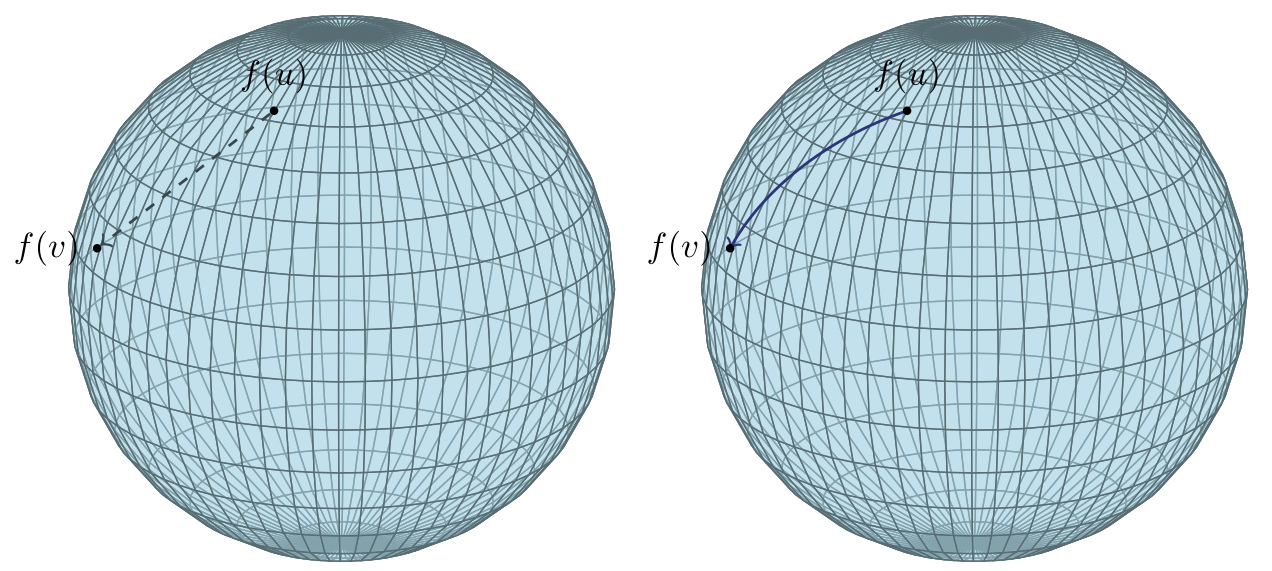
\includegraphics[width=\textwidth]{../\string_build/html/\string_images/mannigfaltigkeit.png}
\caption{Visualisierung zweier unterschiedlicher Abstandsbegriffe für Punkte auf der Kugeloberfläche \(\mathbb{S}^2\).}\label{\detokenize{manifolds/manifolds_prelim:fig-kugel}}\end{figure}

\par
Aus dieser Anschauung wird klar, dass unser bisheriges Konzept von Differenzierbarkeit im Mehrdimensionalen aus dem \href{https://fau-ammn.github.io/MathDataScience2/ableitungen/ableitungen.html}{MP 2 Skript} nicht ausreicht, um auf diesem Objekt geeignet Funktionen abzuleiten.
Da man in vielen Bereichen der Physik und der Mathematik nicht nur auf offenen Teilmengen des \(\R^n\) ableiten möchte, benötigen wir ein analoges Prinzip für topologische Räume \(\M := (\M, \tau)\).

\par
\textbf{Wie können wir den Ableitungsbegriff auf topologische Räume übertragen?}

\par
Die grundlegende Idee ist es, den topologischen Raum \(\M\) lokal mit einer Teilmenge des \(\R^n\) zu identifizieren.
Für eine beliebige offene Teilmenge \(U\subset \M\) betrachten wir also eine Abbildung
\begin{align*}
\phi:U\rightarrow \R^n.
\end{align*}
\par
Wir wollen fordern, dass es sich bei \(\phi\) um eine \emph{injektive Abbildung} handelt, so dass eine inverse Abbildung \(\phi^{-1}\) existiert.
Diese Umkehrabbildung müssen wir jedoch auf das Bild \(\phi(U) \subset \R^n\) einschränken, damit sie wohldefiniert ist.
Damit erhalten wir eine \emph{lokale Bijektion} \(\phi^{-1}:\phi(U)\rightarrow U\).

\par
Betrachten wir nun eine Funktion \(f \colon \M \rightarrow \R^m\), die Punkte des topologischen Raumes auf Punkte des \(\R^m\) abbildet.
Wenn wir diese Funktion differenzieren möchten, so sehen wir ein, dass die Verknüpfung
\begin{align*}
f \circ \phi^{-1} : \phi(U) \subset \R^n \to \R^m
\end{align*}
\par
es uns erlaubt, das Problem der Ableitung in topologischen Räumen auf das Konzept der mehrdimensionalen Differentiation im \(\R^n\) zurückzuführen.


\subsubsection{Karten und Atlanten auf topologischen Räumen}
\label{\detokenize{manifolds/manifolds_prelim:karten-und-atlanten-auf-topologischen-raumen}}
\par
Um den Ableitungsbegriff auf topologischen Räumen \(\M\) formal definieren zu können, benötigen wir zusätzlich zur Bijektivität der Abbildung \(\phi \colon U \rightarrow \phi(U) \subset \R^n\) die Bedingung, dass für jede Teilmenge \(U \subset \M\) gilt,
\begin{align*}
\phi(U)\text{ ist offen} \ \Leftrightarrow \ U \text{ ist offen}.
\end{align*}
\par
Diese Forderung bedeutet, dass offene Teilmengen in \(U \subset \M\) gerade mit offenen Teilmengen in \(\phi(U) \subset \R^n\) identifiziert werden.
Wir wollen im Folgenden beide Implikationsrichtungen diskutieren.

\par
1. \(\phi(U)\) ist offen \(\Rightarrow U \) ist offen.

\par
Diese Implikation ist äquivalent zur Forderung, dass Urbilder offener Mengen selbst wieder offen sind.
Mit \cref{manifolds/manifolds_prelim:def:stetigkeitTopologie} bedeutet dies wiederum, dass die Abbildung \(\phi\) stetig ist.

\par
2. \(\phi(U)\) ist offen \(\Leftarrow U \) ist offen.

\par
Analog zur obigen Überlegung sehen wir ein, dass diese Bedingung gerade aussagt, dass \(\phi^{-1}\) stetig ist.
Diese Forderung ist nicht immer trivialerweise erfüllt.

\par
Das folgende Beispiel zeigt, dass es tatsächlich stetige bijektive Abbildung \(\phi\) gibt, für die gilt, dass die Umkehrabbildung \(\phi^{-1}\) \emph{nicht stetig} ist.
\begin{example}{}{manifolds/manifolds_prelim:ex:nonho}



\par
Wir betrachten in diesem Beispiel die Funktion
\begin{align*}
\phi:[0,2\pi)&\to\R^2,\\
t &\mapsto \phi(t):= (\cos(t), \sin(t)).
\end{align*}
\par
Wir erkennen, dass \(\phi([0,2\pi)) = \S^1\) gerade der Einheitskreis ist, und dass \(\phi:[0,2\pi)\to\S^1\) bijektiv und stetig ist.
Allerdings stellen wir fest, dass die Umkehrabbildung nicht stetig ist.
Sei dazu \((x_i)_{i\in\N}\) eine Folge von Punkten auf dem Einheitskreis \(\S^1\), deren \(y\) Koordinate negativ ist und die gegen den Punkt \(x = (1,0) \in \S^1\) konvergieren, d.h.,
\begin{align*}
\lim_{i\rightarrow\infty} x_i =: x = (1,0) \in \S^1.
\end{align*}
\par
Betrachten wir jedoch den Grenzwert der Folge von Funktionswerten \((\phi^{-1}(x_i))_{i\in I}\), so sehen wir, dass
\begin{align*}
\lim_{i\to\infty} \phi^{-1} (x_i) = 2\pi \neq 0 = \phi^{-1}(x)
\end{align*}
\par
und somit ist \(\phi^{-1}\) offensichtlich nicht stetig.
\end{example}

\begin{figure}[htbp]
\centering


\noindent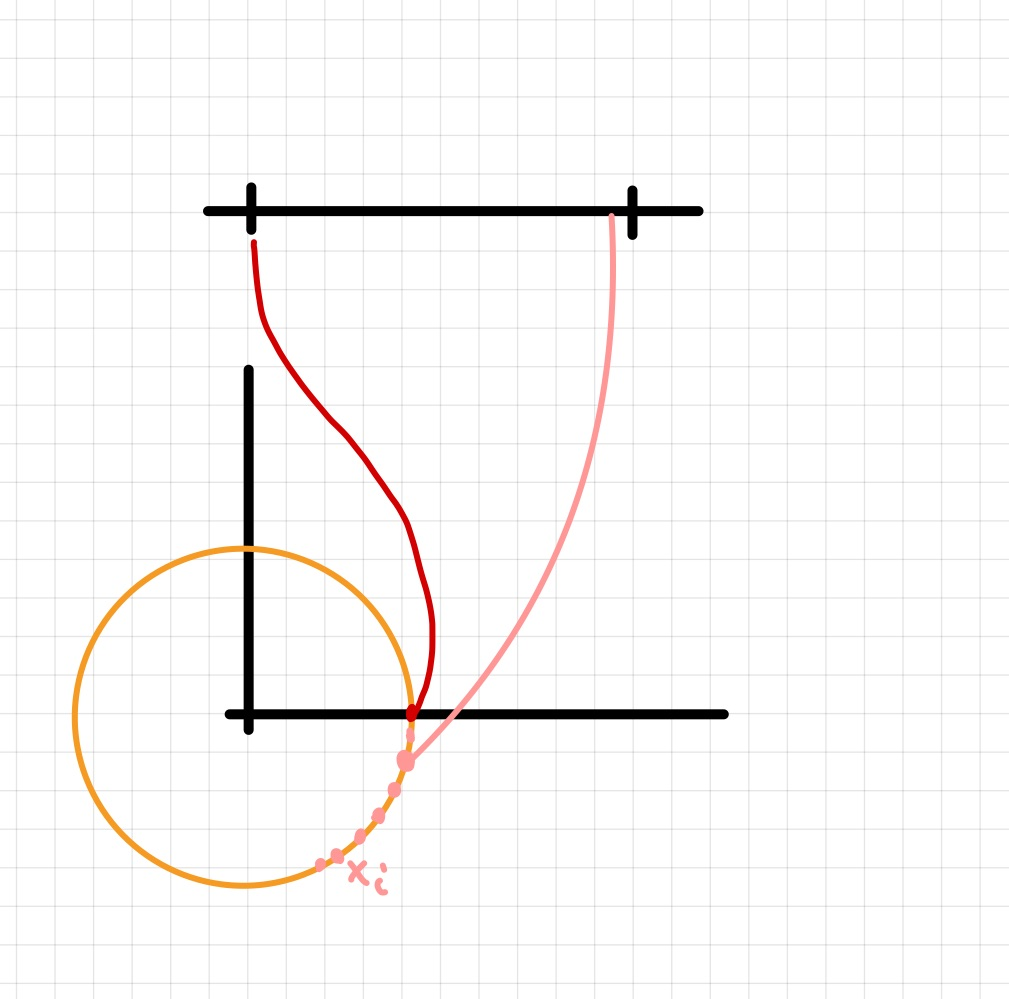
\includegraphics[width=\textwidth]{../\string_build/html/\string_images/nonhomöo.jpg}
\caption{Visualisierung einer unstetigen Umkehrabbildung für das \cref{manifolds/manifolds_prelim:ex:nonho} }\label{\detokenize{manifolds/manifolds_prelim:fig-nonh}}\end{figure}

\par
Insgesamt fordern wir also, dass \(\phi:U\rightarrow\phi(U)\) bijektiv ist und zusätzlich, dass sowohl \(\phi\) als auch die Umkehrabbildung \(\phi^-1\) stetig sind.
Eine solche Abbildung definiert man unter dem Begriff \emph{Homöomorphismus}.
\begin{definition}{(Homöomorphismus)}{manifolds/manifolds_prelim:definition-5}



\par
Seien \(X\) und \(Y\) topologische Räume.
Dann nennen wir eine Abbildung \(f \colon X \rightarrow Y\) einen \textbf{Homöomorphismus}, wenn sie folgende Eigenschaften erfüllt:
\begin{enumerate}

\item {} 
\par
\(f\) ist bijektiv

\item {} 
\par
\(f\) ist stetig

\item {} 
\par
die Umkehrfunktion \(f^{-1}\) ist ebenfalls stetig.

\end{enumerate}
\end{definition}

\par
Speziell im Kontext von Mannigfaltigkeiten \(\M\), als Spezialfall topologischer Räume (wie wir noch sehen werden), nennt man eine offene Menge zusammen mit einem Homöomorphismus eine \textbf{Karte} auf \(\M\).
\begin{definition}{(Karte)}{manifolds/manifolds_prelim:definition-6}



\par
Es sei \(\M\) ein topologischer Raum und \(U\subset\M\) eine offene Menge.
Sei außerdem \(\phi:U\rightarrow \phi(U)\subset \R^n\) ein Homöomorphismus.
Dann heißt das Tupel \((U,\phi)\) \textbf{Karte} auf \(\M\).
\end{definition}

\par
Um einen Ableitungsbegriff für Funktionen \(f:\M\to\R^m\) über eine Karte \((U,\phi)\) und der Verknüpfung \(f\circ \phi^{-1}\) zu definieren benötigen wir noch ein zusätzliches Konzept.
Denn in der Situation, dass \((V,\psi)\) eine zweite Karte ist, deren offene Menge \(V\) einen nichtleeren Schnitt mit der offenen Menge \(U\) hat, d.h., \(U\cap V \neq \emptyset\), erhalten wir genau auf dem Schnitt dieser Mengen zwei unterschiedliche Parametrisierungen,
\begin{align*}
f\circ \phi^{-1} = (f\circ\psi^{-1})\circ(\psi\circ \phi^{-1}),\\
f\circ \psi^{-1} = (f\circ\phi^{-1})\circ(\phi\circ \psi^{-1}).
\end{align*}
\par
Um von einer Karte zur nächsten Karte zu kommen benötigen wir eine geeignete Abbildung.
\begin{definition}{(Kartenwechsel)}{manifolds/manifolds_prelim:definition-7}



\par
Es sei \(\M\) ein topologischer Raum und es seien \((U,\phi)\) und \((V,\psi)\) zwei Karten auf \(\M\) mit nicht leerem Schnitt, d.h., \(U\cap V\neq \emptyset\).
Dann nennt man die Abbildung
\begin{align*}
\psi\circ\phi^{-1}: \phi(U\cap V)\rightarrow \psi(U\cap V)
\end{align*}
\par
einen \textbf{Kartenwechsel} von \((U,\phi)\) nach \((V,\psi)\).
\end{definition}

\begin{figure}[htbp]
\centering


\noindent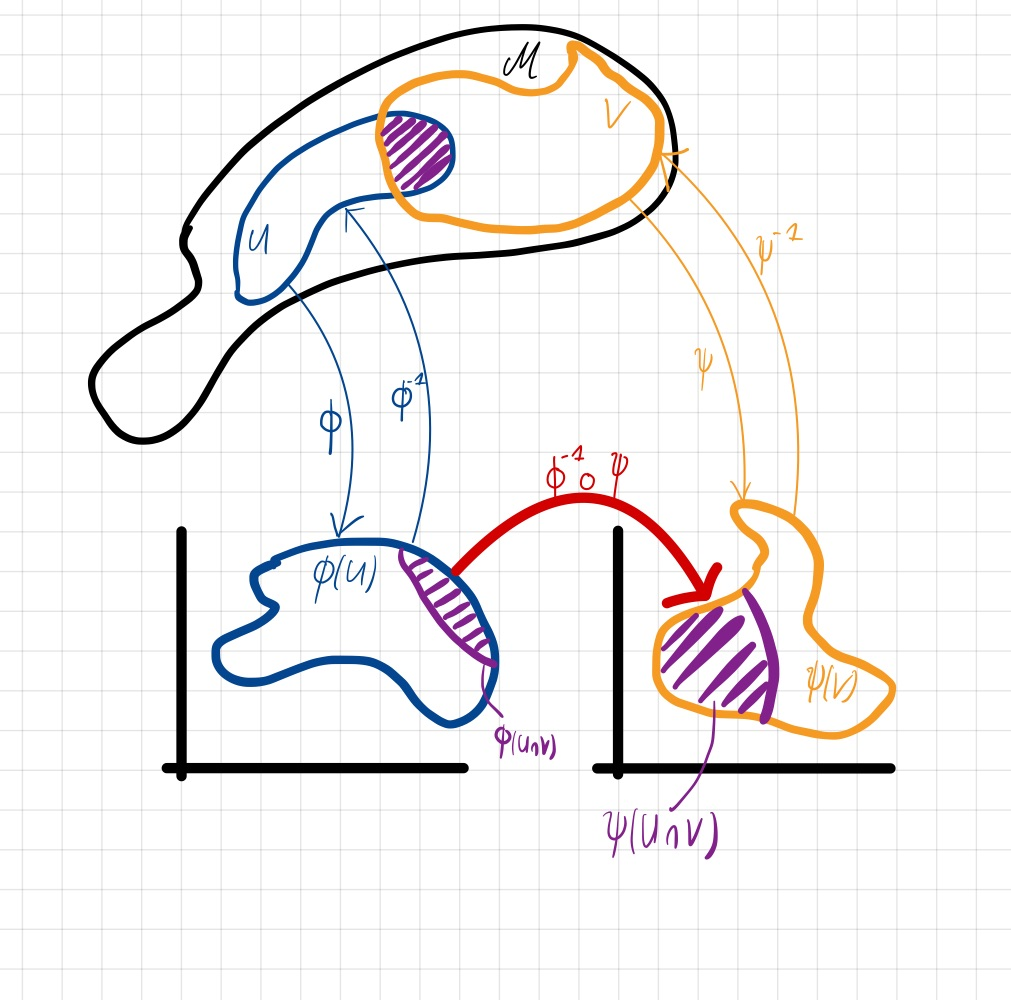
\includegraphics[width=\textwidth]{../\string_build/html/\string_images/chartchange.jpg}
\caption{Kartenwechsel.}\label{\detokenize{manifolds/manifolds_prelim:fig-chartchange}}\end{figure}

\par
Wir erkennen also, dass Umparametrisierungen der Form \(\psi\circ \phi^{-1}\) entscheidend sind, um von einer lokalen Identifikation des topologischen Raums zur nächsten zu gelangen.
Wäre nun der Kartenwechsel \(\psi\circ \phi^{-1}\) und respektive \(\phi\circ \psi^{-1}\) differenzierbar, so könnte man die jeweiligen Ableitungen leicht durch die Kettenregel ineinander umrechnen.
Allerdings existieren durchaus Beispiele, in denen sowohl \(f\circ\phi^{-1}\) als auch \(f\circ\psi^{-1}\) differenzierbar sind, aber der Kartenwechsel \(\psi\circ\phi^{-1}\) nicht.
Deshalb führt man zusätzlich noch den folgenden Begriff ein.
\begin{definition}{(Atlas)}{manifolds/manifolds_prelim:definition-8}



\par
Es sei \(\M\) ein topologischer Raum.
Eine Familie von Karten \(\mathcal{A} = (U_i,\phi_i)_{i\in I}\) indiziert durch die Indexmenge \(I\) heißt \textbf{Atlas}, falls die Vereinigung aller offenen Mengen eine Überdeckung des topologischen Raums darstellt, d.h., es gilt
\begin{align*}
\M = \bigcup_{i\in I} U_i.
\end{align*}
\par
Wir nennen einen Atlas \(k\) mal \textbf{differenzierbar} oder von der Klasse \(C^k\), falls jeder Kartenwechsel \(\phi_i\circ\phi_j^{-1}, i,j\in I\) \(k\) mal stetig differenzierbar ist.
\end{definition}

\par
Die Begriffe \emph{Karte} und \emph{Atlas} stammen in der Tat aus mathematischen Überlegungen in der Kartographie.
Man kann Teile der Erdoberfläche mit einer Karte auf eine Ebene \(\R^2\) abbilden.
Nähert man sich dem Rand einer Karte, so möchte man zu einer anderen Karte wechseln, die das angrenzende Gebiet darstellt.

\par
So kann eine Mannigfaltigkeit durch einen vollständigen Satz von Karten vollständig beschrieben werden; man braucht dabei Regeln, wie sich beim Kartenwechsel die Karten überlappen.


\subsubsection{Differenzierbare Mannigfaltigkeiten}
\label{\detokenize{manifolds/manifolds_prelim:differenzierbare-mannigfaltigkeiten}}
\par
Für einen topologischen Raum \(\M\) können mehrere Atlanten \(\mathcal{A}\) existieren, weshalb es sinnvoll ist Äquivalenzklassen von Atlanten zu betrachten.
\begin{definition}{(\protect\(C^k\protect\) differenzierbare Struktur)}{manifolds/manifolds_prelim:definition-9}



\par
Für einen Index \(k\in \N \cup \{\infty\}\) heißen zwei differenzierbare Atlanten \(\mathcal{A}_1, \mathcal{A}_2\) der Klasse \(C^k\) \textbf{\(k\) äquivalent}, falls ihre Vereinigung \(\mathcal{A}_1\cup \mathcal{A}_2\) wieder ein Atlas der Klasse \(C^k\) ist.
Dies bedeutet insbesondere, dass die Kartenwechsel durch die Vereinigung der beiden Atlanten weiterhin \(k\) mal stetig differenzierbar bleiben.
In diesem Fall notieren wir \(\mathcal{A}_1\sim_k \mathcal{A}_2\).
Die Äquivalenzklasse \([\mathcal{A}]_{\sim_k}\) nennt man eine \textbf{\(C^k\) differenzierbare Struktur}.
\end{definition}

\begin{emphBox}{}{}

\par
\href{https://de.wikipedia.org/wiki/Felix\_Hausdorff}{Felix Hausdorff} (geboren am 8. November 1868 in Breslau; gestorben am 26. Januar 1942 in Bonn) war ein deutscher Mathematiker.
\end{emphBox}

\par
Bisher haben wir \(\M\) als allgemeinen topologischen Raum betrachtet.
In vielen Anwendungen benötigt man aber weitere nützliche Eigenschaften des Raumes.
Insbesondere wenn man \href{https://de.wikipedia.org/wiki/Testfunktion}{glatte Testfunktionen} und \href{https://en.wikipedia.org/wiki/Partition\_of\_unity}{die Zerlegung der Eins} benutzen möchte braucht man folgende zwei zusätzliche Eigenschaften.

\par
Wir definieren zunächst die Eigenschaft eines Hausdorff Raums.
\begin{definition}{(Hausdorff Raum)}{manifolds/manifolds_prelim:def:hausdorffraum}



\par
Ein topologischer Raum \(\M\) heißt \textbf{Hausdorff Raum}, falls für je zwei unterschiedliche Punkte \(x,y\in \M, x\neq y\) offene Umgebungen \(U(x), U(y) \subset \M\) existieren, welche disjunkt sind, d.h., \(U(x)\cap U(y) = \emptyset\).
Man nennt \(\M\) dann auch einen \textbf{separierten Raum}.
\end{definition}

\par
Als zweite nützliche Eigenschaft fordern wir, dass unser topologischer Raum \(\M\) das zweite Abzählbarkeitsaxiom erfüllen soll.
\begin{definition}{(Zweites Abzählbarkeitsaxiom)}{manifolds/manifolds_prelim:definition-11}



\par
Ein toplogischer Raum \((\M, \tau)\) erfüllt das \textbf{zweite Abzählbarkeitsaxiom}, falls \emph{abzählbar} viele offene Mengen \((V_i)_{i\in\N} \in \tau\) existieren, so dass für jeden Punkt \(x\in \M\) und jede offene Umgebung \(U(x) \in \tau\) von \(x\) mindestens ein Index \(k\in\N\) existiert mit \(V_k \subset U(x)\).
Man nennt \((\M, \tau)\) dann auch \textbf{zweitabzählbar}.
\end{definition}

\par
Diese zwei Bedingung wirken zunächst abstrakt.
Glücklicherweise werden sie jedoch von vielen üblichen topologischen Räumen erfüllt, wie zum Beispiel dem Euklidischen Raum \(\R^n\).
\begin{remark}{}{manifolds/manifolds_prelim:remark-12}



\par
Falls der Begriff eines zweitabzählbaren Hausdorff Raums zu unhandlich erscheint, kann man für die meisten Anwendungen in der Physik auch einfach \textbf{metrische Räume} betrachten, die diese beiden Eigenschaften implizieren.
\end{remark}

\par
Nun haben wir alle nötigen Voraussetzungen geschaffen um den Begriff einer Mannigfaltigkeit formal einzuführen.
\begin{definition}{}{manifolds/manifolds_prelim:definition-13}



\par
Es sei \(\M\) ein zweitabzählbarer Hausdorff Raum und für \(k\in\N\cup \{\infty\}\) sei \([\mathcal{A}]_{\sim_k}\) eine \(C^k\) differenzierbare Struktur.
Dann nennen wir \((\M,[\mathcal{A}]_{\sim_k})\) eine \(k\) \textbf{mal differenzierbare Mannigfaltigkeit}.
Für den Spezialfall \(k=\infty\) sprechen wir auch von einer \textbf{glatten Mannigfaltigkeit}.

\par
Falls alle Karten auf \(\M\) nach \(\R^n\) abbilden, so nennt man die Mannigfaltigkeit \emph{\(n\) dimensional}.
\end{definition}

\par
Ähnlich wie bei topologischen Räumen spricht man in den meisten Fällen nur von der Mannigfaltigkeit \(\M\); die differenzierbare Struktur \([\mathcal{A}]_{\sim_k}\) wird dabei implizit vorausgesetzt.

\par
Basierend auf einer differenzierbaren Mannigfaltigkeit \(\M\) können wir nun differenzierbare Funktionen auf \(\M\) definieren.
\begin{definition}{}{manifolds/manifolds_prelim:definition-14}



\par
Sei \(\M\) eine \(k\) mal differenzierbare Mannigfaltigkeit \(\mathcal{A}\) ein Atlas auf \(\M\).
Dann nennen wir eine Abbildung \(f:\M\to\R^m\) \textbf{\(k\) mal differenzierbar}, falls für jeden Punkt \(x\in\M\) eine differenzierbare Karte \((U(x),\phi)\in\mathcal{A}\) existiert, so dass \(f\circ\phi^{-1} \in C^k(\phi(U(x)); \R^m)\).
Insbesondere schreiben wir in diesem Fall \(f\in C^k(\M; \R^m)\).
\end{definition}

\par
In vielen Anwendungen beschränkt man sich nur auf \emph{glatte Mannigfaltigkeiten} und \emph{glatte Funktionen} in \(C^\infty(\M; \R^m)\).
Wir werden im Folgenden der Einfachheit halber auch dazu übergehen.
\begin{lemma}{}{manifolds/manifolds_prelim:lemma-15}



\par
Es sei \(\M\) eine glatte Mannigfaltigkeit.
Dann ist \(C^\infty(\M; \R^m)\) ein reeller Vektorraum mit den Verknüpfungen
\begin{align*}
(\lambda \cdot f)(x) := \lambda\cdot f(x)\text{ für } f\in C^\infty(\M; \R^m), \lambda\in\R,\\
(f + g)(x) := f(x) + g(x)\quad\text{ für } f,g\in C^\infty(\M; \R^m).
\end{align*}\end{lemma}

\begin{proof}
 In der Hausaufgabe zu zeigen.
\end{proof}

\par
Die Eigenschaft der Differenzierbarkeit einer Funktion auf einer Mannigfaltigkeit ist kartenunabhängig, wie folgendes Lemma feststellt.
\begin{lemma}{}{manifolds/manifolds_prelim:lem:differenzierbarkeitKartenunabhaengig}



\par
Es sei \(\M\) eine glatte Mannigfaltigkeit und \(\mathcal{A}\) ein Atlas auf \(\M\).
Außerdem sei \(f:\M \to \R^m\) eine Funktion, \((U,\phi)\in \mathcal{A}\) eine Karte und \(x \in U\) ein Punkt in der offenen Menge \(U\).
Ist \(f\circ\phi^{-1}\) differenzierbar in \(x\), so ist \(f\circ\psi^{-1}\) auch differenzierbar in \(x\) für jede Karte \((V,\psi) \in \mathcal{A}\) mit \(x\in V\).
\end{lemma}

\begin{proof}
 In der Hausaufgabe zu zeigen.
\end{proof}


\section{Tangentialräume und Tangentialbündel}
\label{\detokenize{manifolds/tangential:tangentialraume-und-tangentialbundel}}\label{\detokenize{manifolds/tangential::doc}}

\subsection{Tangentialräume an Mannigfaltigkeiten}
\label{\detokenize{manifolds/tangential:tangentialraume-an-mannigfaltigkeiten}}
\par
Aus dem Kapitel \cref{odestability/ruhelagen:s-linearisierung-ruhelage}  ist bereits das Konzept der \emph{Linearisierung} bekannt.
Anschaulich gesprochen haben wir eine differenzierbare Funktion \(f\) durch ihre Linearisierung ersetzt um ein einfacheres Problem zu erhalten.
Dieses Konzept soll nun auf glatte Mannigfaltigkeiten übertragen werden.

\par
Wir haben bereits erkannt, wie wir den Begriff der Differenzierbarkeit einer Funktion auf einer Mannigfaltigkeit definieren.
Und obwohl die Frage nach der Differenzierbarkeit einer Funktion nach \cref{manifolds/manifolds_prelim:lem:differenzierbarkeitKartenunabhaengig} kartenunabhängig ist, so stellt sich heraus, dass der tatsächliche \emph{Wert der Ableitung} einer Verknüpfung \(f \circ\phi^{-1}\) noch immer von der konkreten Wahl des Homöomorphismus \(\phi\) abhängt.
Um auch hier die gewünschte Kartenunabhängigkeit zu erreichen, brauchen wir einen anderen Begriff der Differenzierbarkeit.
Hierbei wird uns der sogenannte \textbf{Tangentialraum} helfen.
Man kann ihn als eine Linearisierung der Mannigfaltigkeit \(\M\) an einem Punkt \(p\in\M\) interpretieren.

\par
Das folgende Beispiel erklärt anschaulich den Tangentialraum an eine Mannigfaltigkeit.
\begin{example}{}{manifolds/tangential:example-0}



\par
Wir betrachten zunächst den Einheitskreis \(\M = \mathbb{S}^1\) und den Punkt \(p = (1, 0)^T \in \mathbb{S}^1\).
Der Tangentialraum \(T_p\M\) an \(\M\) im Punkt \(p\) ist der eindimensionale Unterraum
\begin{align*}
T_p\M = \lbrace \lambda \cdot (0, 1)^T : \lambda \in \R \rbrace \subset \R^2.
\end{align*}\end{example}

\par
Es gibt in der Literatur zwei verschiedene, jedoch äquivalente Arten den Tangentialraum zu definieren.
\begin{itemize}
\item {} 
\par
\textbf{Geometrischer Tangentialraum}: Bei diesem Ansatz wählt man eine geometrisch Anschauung und definiert den Tangentialraum durch Richtungsvektoren, die am Punkt \(p\in\M\) anliegen.
Der Vorteil dieser Definition ist es, dass sie intuitiv und geometrisch anschaulich ist.

\item {} 
\par
\textbf{Algebraische Defnition}: Bei diesem Ansatz führt man den Tangentialraum mittels spezieller linearer Abbildungen, genannt Derivationen, zurück.
Man verliert hierbei zwar die geometrische Anschauung, allerdings ist das Konzept relativ einfach zu formulieren und hilft die Sachverhalte auf algebraische Zusammenhänge zurückzuführen.

\end{itemize}

\par
In der Praxis (und in vielen Mathematikbüchern) werden beide Definitionen nebeneinander verwendet und die jeweilige Interpretation geht dann aus dem Kontext hervor.
Da sich die beiden Konzepte somit schlecht voneinander trennen lassen werden wir im Folgenden den geometrischen Tangentialraum \(T^{\text{geo}}_p\M\) und den algebraischen Tangentialraum \(T^{\text{alg}}_p\M\) explizit einführen und anschließend eine Isomorphie
\begin{align*}
T^{\text{geo}}_p\M\cong T^{\text{alg}}_p\M
\end{align*}
\par
zwischen den beiden Tangentialräumen zeigen.

\begin{emphBox}{}{}
\par
In der Literatur wird diese explizite Unterscheidung oft nicht vorgenommen.
Stattdessen wird der Tangentialraum einfach nur \(T_p\M\) genannt.
Elemente dieses Raums sind dann je nach Kontext geometrisch oder algebraisch zu interpretieren.
\end{emphBox}


\subsubsection{Geometrische Definition}
\label{\detokenize{manifolds/tangential:geometrische-definition}}
\par
Von der Differentiation im Mehrdimensionalen ist bereits das Konzept der \textbf{Richtungsableitung} bekannt (siehe Kapitel 6.2.2 in \cite{Ten21}).
Hierbei betrachtet man für eine Funktion \(F:\R^n\to\R\) den Strahl \(\gamma(t):= x + t\cdot v\), wobei \(x,v\in\R^n\) und den Grenzwert
\begin{align*}
\lim_{t\to 0} \frac{F(\gamma(t)) - F(\gamma(0))}{t} = \frac{F(x + t\cdot v) - F(x))}{t}.
\end{align*}
\par
Wir werden dieses Konzept nun auf glatte \(n\) dimensionale Mannigfaltigkeiten \(\M\) verallgemeinern, indem wir anstatt von Strahlen differenzierbare \emph{Kurven} auf der Mannigfaltigkeit betrachten.
\begin{definition}{}{manifolds/tangential:definition-1}



\par
Sei \(\M\) eine glatte Mannigfaltigkeit und sei
\begin{align*}
\gamma \colon (-1,1) \rightarrow \M
\end{align*}
\par
eine Kurve auf der Mannigfaltigkeit \(\M\).
Wir nennen \(\gamma\) \textbf{differenzierbar} im Punkt \(0\in(-1,1)\), falls die Kurve \emph{stetig} ist und falls eine Karte \((U,\phi)\) von \(\M\) existiert, so dass für genügend kleines \(\varepsilon\) auch \(\gamma((-\varepsilon,\varepsilon))\subset U\) gilt und die Verknüpfung
\begin{align*}
\phi \circ \gamma:(-\varepsilon,\varepsilon)\to\R^n
\end{align*}
\par
differenzierbar in \(0\) ist .
\end{definition}

\par
Wir werden im Folgenden ausschließlich die Ableitung der Kurve im Punkt \(t=0\) betrachten und sprechen deshalb verkürzt einfach nur von \emph{differenzierbaren} Kurven.
Zusätzlich sei zu bemerken, dass die obige Definition \textbf{nicht} von der Wahl der Karte abhängt.
\begin{example}{}{manifolds/tangential:example-2}



\par
Es sei \(\M=\S^2\) die Einheitssphäre und \(f:\M\to\R\) beschreibe eine Wärmeverteilung auf deren Oberfläche.
Betrachtet man nun die Bahn eines Partikels auf der Oberfläche beschrieben durch die Kurve \(\gamma:(-t, t)\to \M\) so erhalten wir eine eindimensionale Abbildung
\begin{align*}
f\circ\gamma:(-t,t)\to \R,
\end{align*}
\par
die zu jedem Zeitpunkt die Temperatur des Ortes, an dem sich der Partikel befindet, beschreibt.
\end{example}

\begin{figure}[htbp]
\centering


\noindent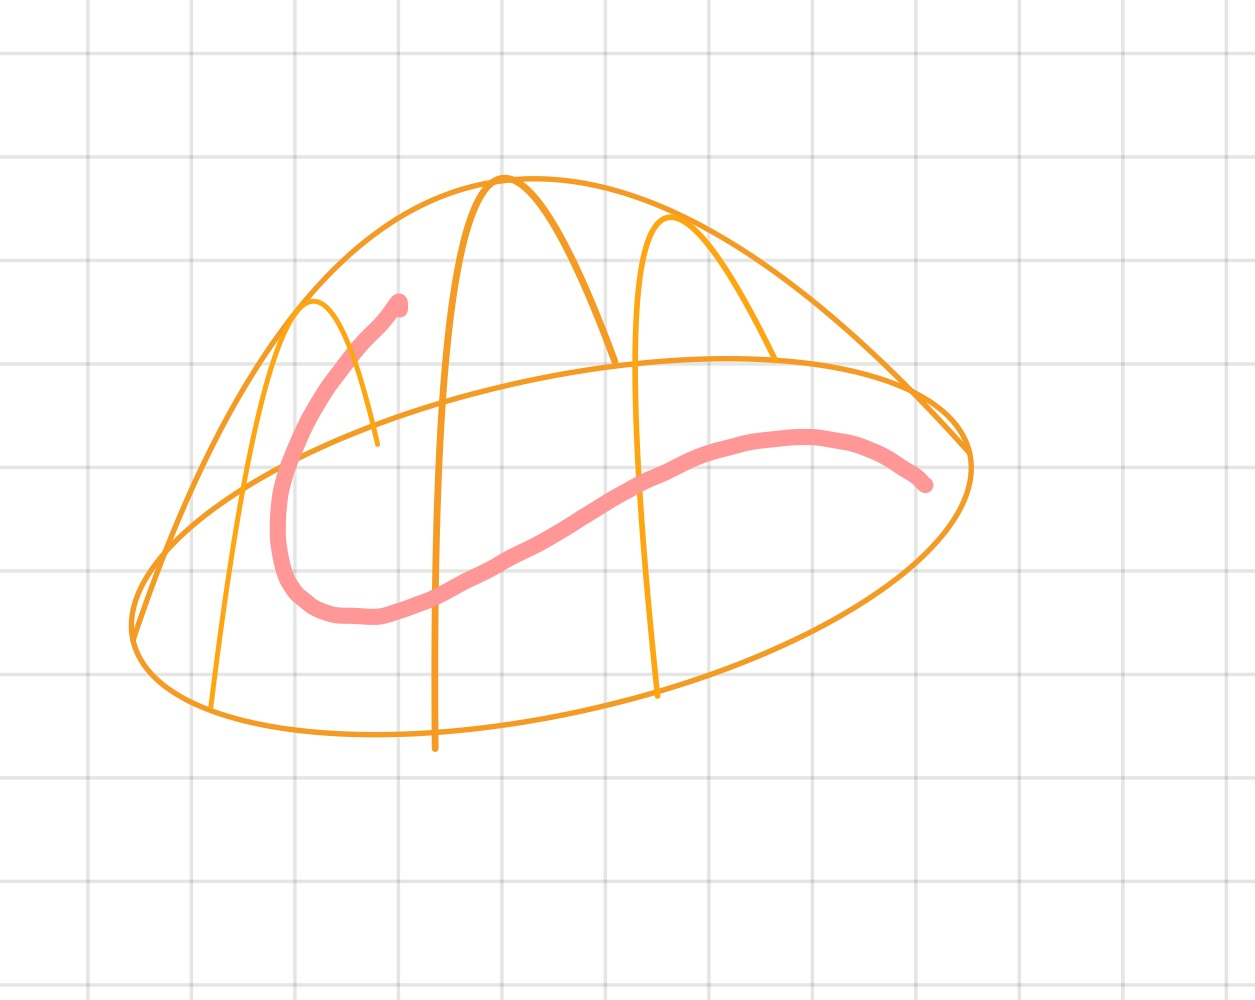
\includegraphics[width=\textwidth]{../\string_build/html/\string_images/velocity.jpg}
\caption{Visualisierung einer Kurve auf der oberen Hälfte der Einheitssphäre im \(\R^3\).}\label{\detokenize{manifolds/tangential:fig-velocity}}\end{figure}

\par
Mit Hilfe von differenzierbaren Kurven auf Mannigfaltigkeiten können wir im Folgenden die Richtungsableitung an einer Mannigfaltigkeit definieren.
\begin{definition}{}{manifolds/tangential:def:direcdiv}



\par
Es sei \(\M\) eine glatte Mannigfaltigkeit, \(\gamma:(-1,1)\to\M\) eine differenzierbare Kurve mit \(\gamma(0)=p\in\M\) und \(f \in C^\infty(\M)\) eine glatte Funktion.
Dann nennen wir die Abbildung
\begin{align*}
D_\gamma : C^\infty(\M) &\to \R\\
f &\mapsto D_\gamma(f):=\frac{d}{dt}(f\circ \gamma)\big\rvert_{t=0}
\end{align*}
\par
\textbf{Richtungsableitung} von \(f\) durch \(\gamma\) im Punkt \(p\).
\end{definition}

\par
Betrachten wir nun eine differenzierbare Kurve \(\gamma \colon (-1, 1) \rightarrow \M\) mit \(\gamma(0)=p \in \M\) und eine glatte Funktion \(f \in \C^\infty(\M)\) definiert auf einer glatten Mannigfaltigkeit \(\M\).
Dann können wir die Richtungsableitung \(D_\gamma(f)\) mit Hilfe der \textbf{Kettenregel für die Differentiation} darstellen als
\begin{align*}
D_\gamma(f) = \frac{d}{dt}(f\circ \gamma)\big\rvert_{t=0} = \frac{d}{dt}\big( (f\circ \phi^{-1}) (\phi \circ \gamma) \big)\rvert_{t=0} = 
\big(D(f\circ \phi^{-1})\big)(\phi(p))\cdot \frac{d}{dt}(\phi \circ \gamma)\rvert_{t=0}
\end{align*}
\par
und für eine weitere differenzierbare Kurve \(\eta \colon (-1, 1) \rightarrow \M\) mit \(\eta(0)=p\) erhalten wir analog
\begin{align*}
D_\eta(f) = \frac{d}{dt}(f\circ \eta)\big\rvert_{t=0} = 
\big(D(f\circ \phi^{-1})\big)(\phi(p))\cdot \frac{d}{dt}(\phi \circ \eta)\rvert_{t=0}.
\end{align*}
\par
Wir erkennen also, dass der Wert der Richtungsableitung in der Tat von der Kurve \(\gamma\) abhängt.
Dies führt auf einen natürlichen Äquivalenzbegriff von Kurven, wie die folgende Bemerkung beschreibt.
\begin{remark}{(Tangentialvektoren)}{manifolds/tangential:rem:tang}



\par
Es sei \(\M\) eine glatte \(n\) dimensionale Mannigfaltigkeit, \(p\in\M\) ein Punkt auf der Mannigfaltigkeit und \((U,\phi)\) eine Karte von \(\M\), für die gilt, dass \(p\in U\) ist.
Für zwei differenzierbare Kurven \(\gamma, \eta:(-1,1) \to U\) mit \(\gamma(0) = \eta(0) = p\) ist die Relation
\begin{align*}
\gamma \sim_p \eta
\qquad \Leftrightarrow \qquad
\frac{d}{dt}(\phi \circ \gamma)\rvert_{t=0} = \frac{d}{dt}(\phi \circ \eta)\rvert_{t=0}\in \R^n
\end{align*}
\par
eine Äquivalenzrelation (siehe Kapitel 2.1.1 in \cite{Bur20}).
Insbesondere ist die Äquivalenzklasse unabhängig von der Wahl des Homöomorphismus \(\phi\).
\end{remark}

\par
Mittels der oben beschriebenen Äquivalenzrelation sind wir in der Lage den Begriff der \emph{Tangentialvektoren} und des \emph{Tangentialraums} zu definieren.
\begin{definition}{}{manifolds/tangential:definition-5}



\par
Es sei \(\M\) eine glatte \(n\) dimensionale Mannigfaltigkeit, \(p\in\M\) ein Punkt auf der Mannigfaltigkeit und \((U,\phi)\) eine Karte von \(\M\), für die gilt, dass \(p\in U\) ist.

\par
Die Äquivalenzklasse \(\gamma^\prime(0):=[\gamma]_{\sim_p}\) wird als \textbf{geometrischer Tangentialvektor} an \(\M\) im Punkt \(p\) bezeichnet.
Der Raum der (geometrischen) Tangentialvektoren
\begin{align*}
T_p^{\text{geo}}\M := \{\gamma^\prime(0): \gamma\text{ ist differenzierbare Kurve mit }\gamma(0)=p\}
\end{align*}
\par
heißt \textbf{geometrischer Tangentialraum} der Mannigfaltigkeit \(\M\) am Punkt \(p \in \M\).
\end{definition}

\par
Der Tangentialraum induziert sogar eine Vektorraumstruktur wie folgende Bemerkung festhält.
\begin{remark}{}{manifolds/tangential:remark-6}



\par
Es sei \(\M\) eine glatte \(n\) dimensionale Mannigfaltigkeit, \(p\in\M\) ein Punkt auf der Mannigfaltigkeit und \((U,\phi)\) eine Karte von \(\M\), für die gilt, dass \(p\in U\) ist.
Sei außerdem \(\gamma \colon (-1,1) \rightarrow \M\) eine differenzierbare Kurve auf \(\M\) mit \(\gamma(0) = p\).
Wir definieren nun die folgende Bijektion auf dem Tangentialraum
\begin{align*}
d\phi\rvert_p \colon T^{\text{geo}}_p\M &\rightarrow \R^n,\\
[\gamma]_{\sim_p} &\mapsto d\phi\rvert_p (\gamma^\prime(0)) := (\phi \circ \gamma)^\prime (0).
\end{align*}
\par
Basierend auf dieser Abbildung lassen sich die folgenden Operationen für den Punkt \(p \in \M\) definieren
\begin{align*}
\gamma^\prime(0) +_{p} \eta^\prime(0) \ &:= \
(d\phi\rvert_p)^{-1}\big[d\phi\rvert_p(\gamma^\prime(0)) + d\phi\rvert_p(\eta^\prime(0))\big]\\
\lambda \cdot_p \gamma^\prime(0) \ &:= \ (d\phi\rvert_p)^{-1} (\lambda \cdot d\phi\rvert_p(\gamma^\prime(0))
\end{align*}
\par
Insgesamt ergibt somit das Tripel \((T_p^{\text{geo}}\M, +_p, \cdot_p)\) einen reellen Vektorraum.
Man bemerke, dass die oben definierten Abbildungen erneut \textbf{unabhängig} von der Wahl des Homöomorphismus \(\phi\) sind.
\end{remark}


\subsubsection{Algebraische Definition}
\label{\detokenize{manifolds/tangential:algebraische-definition}}
\par
Alternativ zur geometrischen Herleitung lässt sich der Tangentialraum auch algebraisch definieren über sogenannte \emph{Derivationen}.
Hierbei beschreiben wir Tangentialvektoren nun nicht mehr als Kurven, sondern als spezielle Funktionale, welche durch ihre Wirkung auf \(C^\infty(\M)\) charakterisiert sind.
Die Motivation hierbei soll die Richtungsableitung aus \cref{manifolds/tangential:def:direcdiv} sein und speziell die im folgenden Lemma beschriebenen Eigenschaften.
\begin{lemma}{}{manifolds/tangential:lemma-7}



\par
Es sei \(\M\) eine glatte Mannigfaltigkeit und \(p\in\M\) und \(\gamma:[-1,1]\to\M\) eine glatte Kurve durch \(p\).
Dann gilt für die Richtungsableitung \(D_\gamma:C^\infty(\M)\to\R\),
\begin{itemize}
\item {} 
\par
\(D_\gamma\in (C^\infty(\M))^\ast\),

\item {} 
\par
Für \(f,g\in C^\infty(\M)\) gilt: \(\ D_\gamma(fg) = D_\gamma(f) g(p) + f(p) D_\gamma(g)\).

\end{itemize}
\end{lemma}

\begin{proof}
 Siehe Übung.
\end{proof}

\par
Die zweite Eigenschaft wird auch \textbf{Produktregel} oder \textbf{Leibnizregel} genannt.
Wir wollen nun im Folgenden nicht nur Richtungsableitungen betrachten, sondern allgemeine Funktionale, die diese Eigenschaft erfüllen.
\begin{definition}{}{manifolds/tangential:definition-8}



\par
Es sei \(\M\) eine glatte Mannigfaltigkeit und \(p\in\M\) ein Punkt der Mannigfaltigkeit.
Wir nennen eine lineare Abbildung \(D: C^\infty(\M) \to \R\) eine \textbf{Derivation} an \(p\), falls sie die folgende Produktregel erfüllt,
\begin{align*}
D(fg) = D(f) g(p) + f(p) D(g).
\end{align*}
\par
Der Raum der Derivationen an \(p\)
\begin{align*}
T^{\text{alg}}_p\M := \{D\in C^\infty(\M)^\ast: D\text{ ist Derivation an }p\}
\end{align*}
\par
wird als \textbf{algebraischer Tangentialraum} bezeichnet.
\end{definition}

\par
Über die Menge der Derivation erhalten wir auf natürliche Art einen Vektorraum da per Definition
\begin{align*}
T^{\text{alg}}_p\M \subset (C^\infty(\M))^\ast
\end{align*}
\par
gilt.
Somit erbt der algebraischer Tangentialraum die Vektorraumoperationen von \(C^\infty(\M)^\ast\) und es muss lediglich nachgeprüft werden, dass diese Teilmenge noch immer ein Vektorraum, also inbesondere abgeschlossen ist.
\begin{lemma}{}{manifolds/tangential:lemma-9}



\par
Es sei \(\M\) eine glatte Mannigfaltigkeit und \(p\in\M\) ein Punkt der Mannigfaltigkeit.
Dann ist \(T^{\text{alg}}_p\M\) ein reeller Vektorraum.
\end{lemma}

\begin{proof}
 Siehe Übung.
\end{proof}

\par
Wie der Name schon erkennen lässt haben Derivationen gewisse Eigenschaften, die von der Ableitungsoperation bekannt sind.
So bildet zum Beispiel jede Derivation konstante Funktionen auf \(0\) ab, wie das folgende Lemma zeigt.
\begin{lemma}{(Derivation konstanter Funktionen)}{manifolds/tangential:lem:constder}



\par
Es sei \(\M\) eine glatte Mannigfaltigkeit und \(p\in\M\) ein Punkt der Mannigfaltigkeit.
Außerdem sei \(f\in C^\infty(\M)\) eine konstante Funktion, d.h., es existiert eine Konstante \(c\in\R\), so dass
\begin{align*}
f(q) = c\quad\forall q\in\M.
\end{align*}
\par
Dann gilt schon \(D(f)=0\) für alle Derivationen \(D\in T^{\text{alg}}_p\M\).
\end{lemma}

\begin{proof}
 Es sei \(D\in T^{\text{alg}}_p\M\) eine beliebige Derivation an den Punkt \(p \in \M\).
Wir betrachten zunächst die konstante Einsfunktion
\begin{align*}
g:\M &\to \R\\
q &\mapsto g(x) := 1.
\end{align*}
\par
Dann gilt mit der Produktregel für Derivationen
\begin{align*}
D(g) = D(g\cdot g) = D(g)\,g(p) + g(p)\, D(g) = 2\,D(g)
\end{align*}
\par
und somit muss schon \(D(g) = 0\) gelten.
Wir können die konstante Funktion \(f\) nun darstellen als \(f= c\,g\) und unter Ausnutzung der Linearität von \(D\) erhalten wir schon
\begin{align*}
D(f) = D(c\,g) = c\,D(g) = 0.
\end{align*}\end{proof}

\par
Wir haben nun zwei verschiedene Arten gesehen den Tangentialraum einzuführen.
Tatsächlich sind diese Definitionen äquivalent in dem Sinn, dass ein Isomorphismus zwischen dem geometrischen und algebraischen Tangentialraum existiert.
\begin{theorem}{(Isomorphie zwischen alg. und geom. Tangentialraum)}{manifolds/tangential:theorem-11}



\par
Es sei \(\M\) eine glatte Mannigfaltigkeit und \(p\in\M\) ein Punkt der Mannigfaltigkeit.
Dann gilt die folgende Isomorphie
\begin{align*}
T^{\text{geom}}_p\M \ \cong \ T^{\text{alg}}_p\M.
\end{align*}\end{theorem}

\begin{proof}
 Siehe z.B. Kapitel 2.3 in \cite{Janich03}.
\end{proof}


\subsubsection{Basis des algebraische Tangentialraums}
\label{\detokenize{manifolds/tangential:basis-des-algebraische-tangentialraums}}\label{\detokenize{manifolds/tangential:sec-tpbasis}}
\par
Wir wollen in diesem Abschnitt eine Basis des algebraischen Tangentialraums konstruieren.
Im Euklidischen Raum können wir auf natürliche Art die Koordinatenrichtungen als Kurven wählen, also Funktionen der Form
\begin{align*}
t \mapsto t e_i
\end{align*}
\par
für \(i=1,\ldots,n\), wobei \(e_i\) den \(i\) ten Einheitsvektor in \(\R^n\) bezeichnet.
Um diese Idee auf Mannigfaltigkeiten zu übertragen wählen wir eine Karte \(\varphi:\M\to\R^n\), wobei man hier auch von
\begin{align*}
\varphi = (\varphi_1,\ldots,\varphi_n) =: (x^1,\ldots,x^n)
\end{align*}
\par
als einem \textbf{lokalen Koordinatensystem} spricht.
Wir erhalten somit Kurven
\begin{align*}
\gamma_{x^i}(t):= \varphi^{-1}(\varphi(p) + t e_i)
\end{align*}
\par
und mithilfe der Richtungsableitung aus \cref{manifolds/tangential:def:direcdiv} die Derivationen
\begin{align*}
\partial_{x^i}^p: C^\infty(\M) &\to \R\\
f &\mapsto \partial_{x^i}^p(f) := \frac{d}{dt} (f\circ \gamma_{x^i}(t)).
\end{align*}\begin{definition}{}{manifolds/tangential:definition-12}



\par
Sei \(\M\) eine glatte \(n\) dimensionale Mannigfaltigkeit für \(n\in\N\) und sei \(f \in C^\infty(\M)\) eine glatte Funktion.
Dann bezeichnen wir die Derivationen
\begin{align*}
\partial_{x^i}^p (f) := \frac{d}{dt} (f\circ \gamma_{x^i}(t)), \quad i=1,\ldots,n
\end{align*}
\par
als \textbf{partielle Derivationen} von \(f\) im Punkt \(p \in \M\).
\end{definition}

\par
Wir interpretieren also im Folgenden das Symbol \(\partial_{x^{i}}^p\) als Derivation an \(p\in\M\), d.h., insbesondere als lineare Abbildung von \(C^\infty(\M)\) nach \(\R\).
Diese partiellen Derivationen folgen der Intuition, dass die partielle Ableitung in eine Richtung auch nur Änderungen in diese Richtung respektiert.
Wir formalisieren diese Anschauung in folgendem Lemma.
\begin{lemma}{}{manifolds/tangential:lem:partderkron}



\par
Es sei \(\M\) eine glatte Mannigfaltigkeit, \(p\in\M\) ein Punkt der Mannigfaltigkeit und \((U,\varphi)\) sei eine Karte mit \(p\in U\).
Dann gilt für die partielle Derivation
\begin{align*}
\partial_{x^i}^p(\varphi_j) = \delta_{ij},
\end{align*}
\par
wobei \(\delta_ij\) das \emph{Kronecker Delta} bezeichnet.
\end{lemma}

\begin{proof}
 Wir betrachten zunächst die Funktion \(\varphi_j \circ \gamma_{x^i}\) und erhalten für \(t\in [-1,1]\)
\begin{align*}
\varphi_j \circ \gamma_{x^i}(t)
&= \varphi_j \circ \varphi^{-1}(\varphi(p) + t e_i)\\
&= (\varphi(p) + t e_i)_j\\ 
&=
\begin{cases}
\varphi(p) + t e_i &\text{ für } i=j,\\
\varphi_j(p)&\text{ sonst}.
\end{cases}
\end{align*}
\par
Somit gilt schon für die partielle Derivation
\begin{align*}
\partial_{x^i}^p(\varphi_j)=
\frac{d}{dt} (\varphi_j \circ \gamma_{x^i}(t)) = 
\begin{cases}
1&\text{ für } i=j,\\
0&\text{ sonst}.
\end{cases}
\end{align*}\end{proof}

\par
Das folgende Hauptresultat dieses Abschnitts erlaubt es uns beliebige Derivationen mithilfe der partiellen Derivationen darzustellen, da diese eine Basis des algebraischen Tangentialraums bilden.
\begin{theorem}{}{manifolds/tangential:thm:tanbasis}



\par
Es sei \(\M\) eine \(n\) dimensionale glatte Mannigfaltigkeit.
Dann bildet die Menge
\begin{align*}
\{\partial_{x^1}^p,\ldots,\partial_{x^n}^p\}
\end{align*}
\par
eine Basis des algebraischen Vektorraums \(T^{\text{alg}}_p\).
Insbesondere gilt
\begin{align*}
\dim(T^{\text{alg}}_p)=\dim(T^{\text{geom}}_p)=n
\end{align*}\end{theorem}

\begin{proof}
 Es sei \((U,\varphi)\) eine Karte der Mannigfaltigkeit \(\M\) und wir nehmen ohne Beschränkung der Allgemeinheit an, dass \(\varphi(p)=0 \in \R^n\) gilt, was stets durch eine entsprechende Translation des Koordinatensystems erreicht werden kann.
Zusätzlich wählen wir einen Radius \(r>0\) klein genug, so dass \(B_r(0) \subset \varphi(U)\) gilt und betrachten als Karte \(\tilde{\varphi} := \varphi\rvert_{\tilde{U}}\), d.h., die Einschränkung von \(\varphi\) auf \(\tilde{U}:= \varphi^{-1}(B_r(0))\).
Wir können die Karte \(\tilde{\varphi}\) wegen der Kartenunabhängigkeit des Tangentialraums und der Tatsache, dass \((\tilde{U},\tilde{\varphi})\) auch eine Karte der Mannigfaltigkeit \(\M\) mit \(p\in \tilde{U}\) ist, betrachten.
Da das Bild von \(\tilde{\varphi}\) nun der gesamte Ball \(B_r(0) \subset \R^n\) ist, können wir nun Strecken von \(0\) zu einem beliebigen Punkt in \(B_r(0)\) betrachten, welche selbst ganz im Bild von \(\tilde{\varphi}\) enthalten sind.

\par
Sei nun \(f\in C^\infty(\M)\) eine beliebige glatte Funktion.
Dann definieren wir die Funktion \(g:= f\circ \tilde{\varphi}^{-1}\) für die insbesondere \(g\in C^\infty(\R^n)\) gilt.
Für einen beliebigen Punkt \(q\in\tilde{U}\) erhalten wir einen Richtungsvektor \(z:=\tilde{\varphi}(q)\in B_r(0)\) und können somit die Einschränkung von \(g\) auf die eindimensionale Strecke zwischen \(0\) und \(z\) in \(\R^n\) betrachten, d.h.,
\begin{align*}
\tilde{g}:[0,1] &\to\R\\
t&\mapsto g(t\cdot z).
\end{align*}
\par
Hierbei sieht man erneut ein, dass \(\tilde{g}\in C^\infty([0,1])\) gilt.
Dies bedeutet insbesondere, dass wir den \emph{Hauptsatz der Differential  und Integralrechnung} (vgl. Theorem 5.3 in \cite{Ten21}) anwenden können und somit erhalten wir
\begin{align*}
\tilde{g}(1) = \tilde{g}(0) + \int_{0}^1 \tilde{g}^\prime(t)\,\mathrm{d}t.
\end{align*}
\par
Wir berechnen die Ableitung im Integral als Richtungsableitung und erhalten,
\begin{align*}
\int_{0}^1 \tilde{g}^\prime(t) \,\mathrm{d}t
=\int_{0}^1 \langle \nabla g (t\cdot z), z \rangle \,\mathrm{d}t
=\sum_{i=1}^{n} \int_{0}^1  \partial_i g (t\cdot z) \cdot z_i \,\mathrm{d}t.
\end{align*}
\par
Da per Definition
\begin{align*}
\tilde{g}(1) = g(z)=f(q)
\end{align*}
\par
und
\begin{align*}
\tilde{g}(0) = g(0) = g(\varphi(p))=f(p)
\end{align*}
\par
gilt, folgt daraus
\begin{align*}
f(q) = 
f(p) + 
\sum_{i=1}^{n} \varphi_i(q)\ \cdot \underbrace{\int_{0}^1  \partial_i (f\circ \varphi^{-1})(t\cdot \varphi(q)) \, \mathrm{d}t}_{:=F_i(q)}.
\end{align*}
\par
An diesem Punkt bemerken wir, dass \(f\circ \varphi^{-1} \in C^\infty(\R^n)\) eine klassisch differenzierbare Funktion ist, wobei \(f\) eine glatte Funktion auf der Mannigfaltigkeit \(\M\) darstellt.
Wenden wir nun die \(j\) te partielle Derivation auf \(f\) an, erhalten wir unter Ausnutzung der Linearität der Abbildung \(\partial_{x^j}^p\)
\begin{align*}
\partial_{x^j}^p (f) = 
\underbrace{\partial_{x^j}^p (f(p))}_{=0} + 
\sum_{i=1}^{n} \partial_{x^j}^p(\varphi_i \cdot F_i) = 
\sum_{i=1}^{n} \partial_{x^j}^p(\varphi_i \cdot F_i)
\end{align*}
\par
wobei wir \cref{manifolds/tangential:lem:constder} und die Tatsache, dass \(\varphi_i, F_i\in C^\infty(\M)\) gilt, benutzt haben.
Weiterhin gilt wegen der Leibnizregel
\begin{align*}
\partial_{x^j}^p(\varphi_i \cdot F_i(q)) = 
\underbrace{\partial_{x^j}^p(\varphi)}_{=\delta_{ij}} F_i(p)+ \underbrace{\varphi_i(p)}_{=0} \partial_{x^j}^p(F_i),
\end{align*}
\par
wobei wir \cref{manifolds/tangential:lem:partderkron} und \(\varphi(p)=0\) verwendet haben.
Somit folgt schon
\begin{align*}
\partial_{x^j}^p (f) = F_j(p)
\end{align*}
\par
und damit insbesondere
\begin{align*}
f = f(p) + \sum_{i=1}^{n} \varphi_i \partial_{x^i}^p(f).
\end{align*}
\par
Dies bedeutet aber schon, dass die partiellen Derivationen ein \textbf{Erzeugendensystem} des algebraischen Tangentialraums bilden, denn sei \(D\in T^{\text{alg}}_p\) eine beliebige Derivation, dann gilt
\begin{align*}
D(f) = \underbrace{D(f(p))}_{=0} + \sum_{i=1}^n D(\varphi_i) \partial_{x^i}^p(f).
\end{align*}
\par
Dies bedeutet, dass jede Derivation \(D\) über eine Linearkombination aus partiellen Derivationen dargestellt werden kann, wobei die Koeffizienten durch \(D(\varphi_i)\) gegeben sind.

\par
Es bleibt die Eindeutigkeit der Darstellung zu zeigen.
Seien dazu Koeffizienten \(\alpha_i \in \R, i=1,\ldots,n\) gegeben, so dass für jede Funktion \(f\in C^\infty(\M)\) gilt
\begin{align*}
D:= \sum_{i=1}^n \alpha_i \partial_{x^i}^p(f) = 0.
\end{align*}
\par
Durch erneute Anwendung von \cref{manifolds/tangential:lem:partderkron} erhalten wir aber, dass
\begin{align*}
0 = D(\varphi_j) = \alpha_j\end{align*}
\par
für alle \(j=1,\ldots,n\) und somit haben wir die \textbf{lineare Unabhängigkeit} bewiesen.

\par
Insgesamt bilden also die partiellen Deriviationen eine Basis des algebraischen Tangentialraums und es gilt
\begin{align*}
\dim(T^{\text{alg}}_p)=\dim(T^{\text{geom}}_p)=n.
\end{align*}\end{proof}


\subsubsection{Kotangentialraum}
\label{\detokenize{manifolds/tangential:kotangentialraum}}
\par
Da wir den Tangentialraum \(T^{\text{alg}}_p\) als Vektorraum identifiziert haben, können wir auch dessen algebraischen Dualraum in der folgenden Definition betrachten.
\begin{definition}{}{manifolds/tangential:definition-15}



\par
Es sei \(\M\) eine glatte Mannigfaltigkeit.
Dann bezeichnen wir mit
\begin{align*}
T_p^\ast\M:= (T_p^{\text{alg}}\M)^\ast
\end{align*}
\par
den algebraischen Dualraum des Tangentialraums, welcher häufig \textbf{Kotangentialraum} genannt wird.
\end{definition}
\begin{remark}{}{manifolds/tangential:remark-16}



\par
Ein Element \(\delta\in T_p^\ast\M\) ist also eine lineare Abbildung
\begin{align*}
\delta: T_p^{\text{alg}}\M \to \R,
\end{align*}
\par
die eine Derivation \(D\in C^\infty(\M)^\ast\) auf eine reelle Zahl \(\delta(D)\in\R\) abbildet.
\end{remark}

\par
Die folgende Definition beschreibt ein wichtiges Element des Kotangentialraums.
\begin{definition}{}{manifolds/tangential:def:totdiff}



\par
Sei \(f\in\C^\infty(\M)\) eine beliebige glatte Funktion auf einer Mannigfaltigkeit \(\M\).
Dann bezeichnen wir das Element \(\mathrm{d}f_p \in T_p^\ast\M\) mit
\begin{align*}
\mathrm{d}f_p: T_p^{\text{alg}}\M &\to\R\\
D_p &\mapsto \mathrm{d}f_p(D):= D_p(f).
\end{align*}
\par
als \textbf{totales Differential} der Funktion \(f\) im Punkt \(p \in \M\).
\end{definition}

\par
Insbesondere können wir das totale Differential \(df\) mit einer glatten Funktion aus \(C^\infty(M)\) identifizieren, was den Zusammenhang von \(T^\ast_p \M\) als Bidualraum von \(C^\infty(\M)\) unterstreicht.

\par
Die Basis von \(T^\ast_p\) wird kanonisch als duale Basis (siehe \cref{vektoranalysis/multilinear:lem:dualeBasis}  gewählt.
Jeder Vektor \(v\in T_p^{\text{alg}}\M\) hat somit eine eindeutige Darstellung
\begin{align*}
v = \sum_{i=1}^n \alpha_i \partial_{x^i}.
\end{align*}
\par
Wir wählen nun Abbildungen \(\mathrm{d}x^i\in T^\ast_p\M, i=1,\ldots,n\) gerade so, dass
\begin{align*}
\mathrm{d}x^i(v) = \alpha_i
\end{align*}
\par
gilt.
Das folgende Lemma zeigt, dass es sich hierbei um eine Basis von \(T^\ast_p\M\) handelt.
\begin{lemma}{}{manifolds/tangential:lemma-18}



\par
Es sei \(\M\) eine glatte Mannigfaltigkeit und \(p\in\M\).
Dann ist die Menge
\begin{align*}
\{\mathrm{d}x^1,\ldots, \mathrm{d}x^n\}
\end{align*}
\par
eine Basis von \(T_p^\ast\M\).
\end{lemma}

\begin{proof}
 Die Aussage folgt direkt aus \cref{vektoranalysis/multilinear:lem:dualeBasis} 
\end{proof}


\subsection{Tangentialbündel}
\label{\detokenize{manifolds/tangential:tangentialbundel}}
\begin{emphBox}{}{}{Bemerkung:}
\par
Im Folgenden bezeichne \(T_p\M\in\{T^{\text{alg}}_p\M, T^{\text{geom}}_p\M \}\) entweder den \emph{algebraischen} oder den \emph{geometrischen Tangentialraum}.
Die konkrete Wahl wird an den entsprechenden Stellen (wenn nötig) spezifiziert.
\end{emphBox}

\par
Bisher haben wir für eine \(n\) dimensionale glatte Mannigfaltigkeit \(\M\) für jeden einzelnen Punkt \(p\in\M\) den zugehörigen Tangentialraum \(T_p\M\) betrachtet, welcher wiederum wegen \cref{manifolds/tangential:thm:tanbasis} isomorph zum \(\R^n\) ist.
Wir interessieren uns jetzt dafür, wie sich Tangentialräume für verschiedene Punkte \(p,q\in \M\) in Beziehung setzen lassen.
Darüber hinaus wollen wir eine globale Struktur definieren welche alle Tangentialräume (d.h. für jedes \(p\in\M\)) zusammenfasst.

\par
In diesem Kontext spricht man von der Mannigfaltigkeit häufig als dem \textbf{Basisraum} \(B=\M\), da die Punkte \(p \in \M\), welche die Vektorräume erzeugen, aus diesem Raum entnommen werden.
Ein erster Ansatz für eine globale Struktur ist die Vereinigung
\begin{align*}
\bigcup_{p\in\M} T_p\M.
\end{align*}
\par
Wir wollen diese Idee im folgenden Beispiel veranschaulichen.
\begin{example}{(Tangentialräume an Einheitskreis)}{manifolds/tangential:ex:tangentialS1}



\par
Sei als zu Grunde liegende Mannigfaltigkeit der Einheitskreis \(\M = \mathbb{S}^1\subset\R^2\) gegeben.
Wir wählen als Repräsentanten für jeden Punkt
\begin{align*}
p=(\cos(\alpha), \sin(\alpha))\in\M, \quad \alpha\in (0,2\pi) \setminus \{\pi\}
\end{align*}
\par
die Kurve
\begin{align*}
\gamma_p(t) := p - t \cdot\big(1, \frac{\cos(\alpha)}{\sin(\alpha)}\big),
\end{align*}
\par
und somit erhalten wir anschaulich die in \hyperref[\detokenize{manifolds/tangential:fig-bundlea}]{Abb.\@ \ref{\detokenize{manifolds/tangential:fig-bundlea}}} für einige Punkte visualisierte Menge.

\par
Es fällt auf, dass sich zwar einzelne Kurven schneiden können, jedoch die Kurven selbst und die assoziierten Vektorräume nicht gleich sind.
Um diese Tatsache zu verdeutlichen ist es praktisch die \emph{disjunkte Vereinigung}
\begin{align*}
\bigsqcup_{p\in\M} T_p\M := \bigcup_{p\in\M} \{p\} \times T_p\M \cong \bigcup_{p\in\M} \{p\} \times \R
\end{align*}
\par
zu betrachten.
Für den Einheitskreis erhalten wir durch die Isomorphie \(T_p\M \cong \R\) so den Zylinder in \hyperref[\detokenize{manifolds/tangential:fig-bundleb}]{Abb.\@ \ref{\detokenize{manifolds/tangential:fig-bundleb}}}.
\end{example}

\begin{figure}[htbp]
\centering


\noindent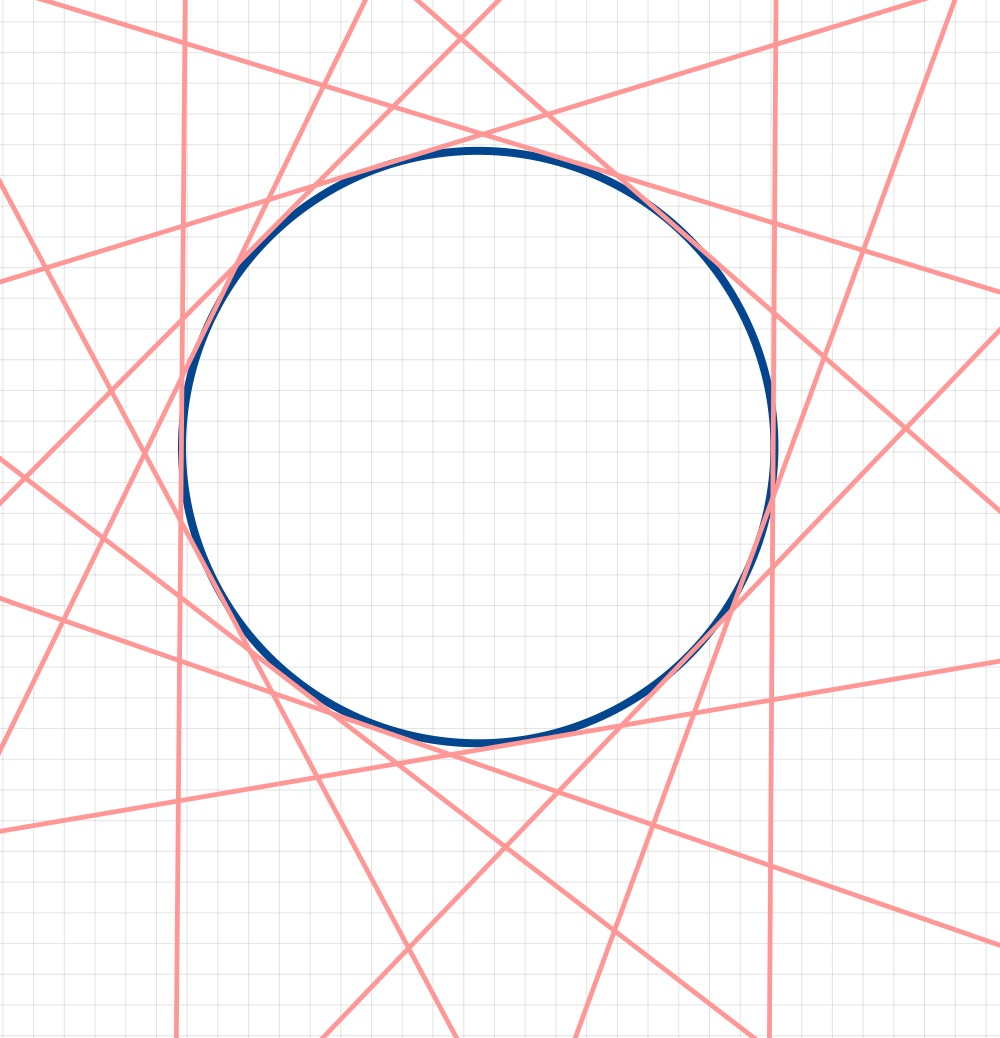
\includegraphics[width=\textwidth]{../\string_build/html/\string_images/bundlea.jpg}
\caption{Visualisierung der Tangentialräume einiger Punkte am Einheitskreises.}\label{\detokenize{manifolds/tangential:fig-bundlea}}\end{figure}

\begin{figure}[htbp]
\centering


\noindent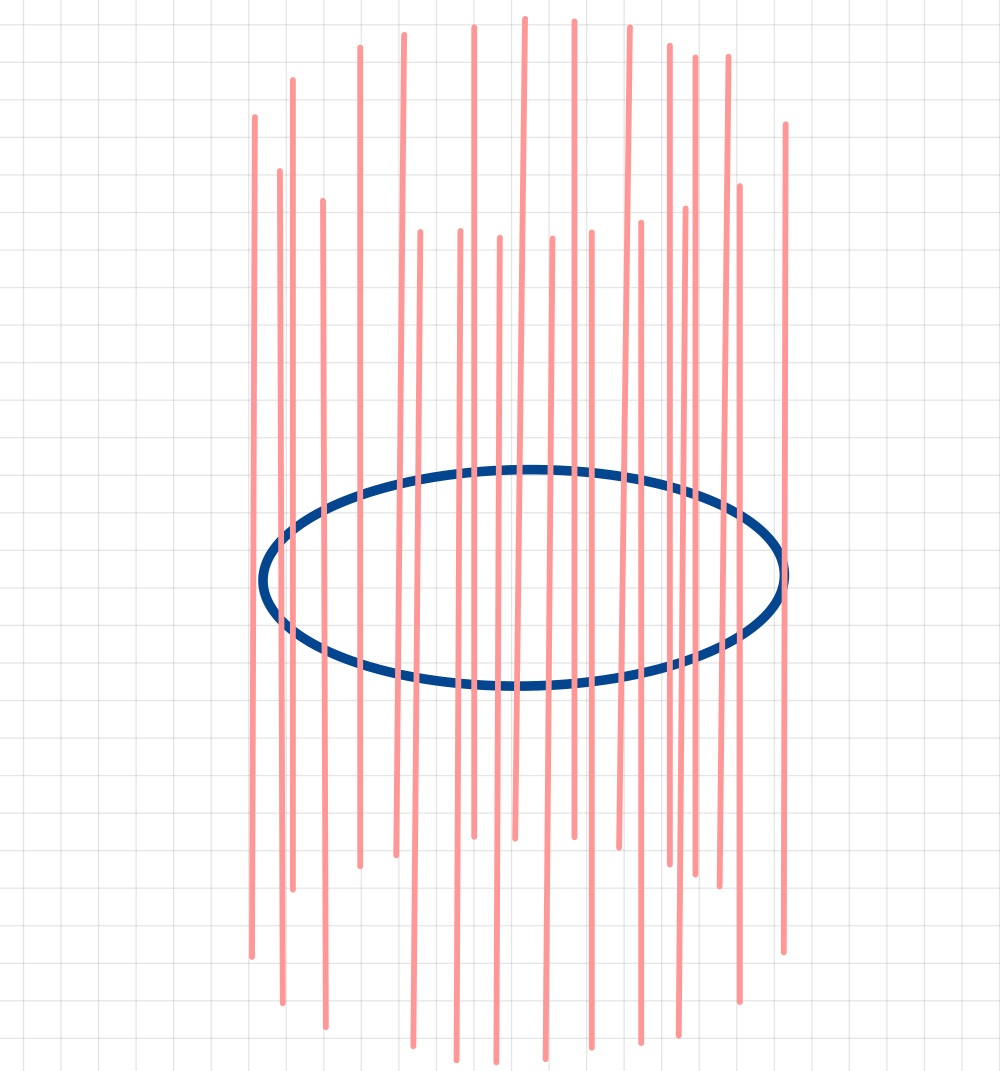
\includegraphics[width=\textwidth]{../\string_build/html/\string_images/bundleb.jpg}
\caption{Visualisierung der disjunkt vereinigten Tangentialräume einiger Punkte am Einheitskreises.}\label{\detokenize{manifolds/tangential:fig-bundleb}}\end{figure}

\par
Wir wollen diese globale Struktur der disjunkten Vereinigung formal definieren.
\begin{definition}{}{manifolds/tangential:definition-20}



\par
Es sei \(\M\) eine glatte Mannigfaltigkeit.
Dann heißt die Menge
\begin{align*}
T\M := \bigsqcup_{p\in\M}  T_p\M = \bigcup_{p\in\M} \{p\} \times T_p\M
\end{align*}
\par
zusammen mit der Projektion
\begin{align*}
\pi:T\M &\to \M\\
\{p\}\times T_p\M &\mapsto p
\end{align*}
\par
das \textbf{Tangentialbündel} von \(\M\).
\end{definition}

\par
Insbesondere erkennen wir, dass wir mit Hilfe der Projektion \(\pi\) jedem Element des Tangentialbündels eindeutig den zu Grunde liegenden Punkt \(p\in\M\) zuordnen können, der den entsprechenden Tangentialraum erzeugt hat.

\par
Im Folgenden wollen wir uns zwei Beispiele für Tangentialbündel an Mannigfaltigkeiten ansehen.
\begin{example}{(Tangentialbündel)}{manifolds/tangential:example-21}





\par
1. Sei \(\M=\R^n\).
Dann ist das Tangentialbündel gerade gegeben durch
\begin{align*}
T\M = \R^n\times\R^n = \R^{2n}.
\end{align*}


\par
2. Wie bereits in \cref{manifolds/tangential:ex:tangentialS1} gesehen erhalten wir für \(\M=\mathbb{S}^1\) als Tangentialbündel den unendlich hohen Zylinder
\begin{align*}
T\M = \mathbb{S}^1\times \R.
\end{align*}\end{example}

\par
In den bisher betrachten Beispielen haben wir als Tangentialbündel jeweils eine Menge der Form \(\M\times \R^n\) erhalten.
Dies ist jedoch nicht immer der Fall wie wir sehen werden.
Tatsächlich bilden Tangentialbündel von dieser Form eine spezielle Unterklasse.
\begin{definition}{}{manifolds/tangential:definition-22}



\par
Sei \(\M\) eine glatte \(n\) dimesnionale Mannigfaltigkeit.
Das Tangentialbündel \(T\M\) heißt \textbf{trivial}, falls gilt
\begin{align*}
T\M\cong \M\times\R^n.
\end{align*}
\par
In diesem Fall nennt man die Mannigfaltigkeit \(\M\) auch \textbf{parallelisierbar}.
\end{definition}
\begin{remark}{}{manifolds/tangential:remark-23}



\par
Es lässt sich zeigen, dass \(\mathbb{S}^1, \mathbb{S}^3,\mathbb{S}^7\) die \emph{einzigen} paralleslisierbaren Sphären sind (siehe \cite{Lee03}).
Die Tatsache, dass \(\mathbb{S}^2\) nicht parallelisierbar ist wird beim Satz vom gekämmten Igel in {prf:ref broken reference}\{TODO\} erneut auftauchen.
\end{remark}

\par
Wir wollen uns nun mit der Frage beschäftigen, wie sich die Tangentialräume für unterschiedliche Punkte \(p,q\in B\) des Basisraums zueinander verhalten, insbesondere wenn \(p\) und \(q\) nahe beieinander liegen.
Hierbei hilft es das abstrakte Konzept eines \textbf{Vektorbündels} zu betrachten.
\begin{definition}{}{manifolds/tangential:definition-24}



\par
Es seien \(\M\) (der sog. Basisraum) und \(E\) (der sog. Totalraum) zwei glatte Mannigfaltigkeiten und \(\pi:E\to \M\) sei glatt und bijektiv. Weiterhin gelte
Außerdem sei \(\pi:E\to \M\) eine glatte und bijektive Abbildung.
Weiterhin gelte
\begin{itemize}
\item {} 
\par
für jeden Punkt \(p\in \M\) sei die sogenannte \textbf{Faser} \(E_p:= \pi^{-1}(p)\) ein \(n\) dimensionaler Vektorraum,

\item {} 
\par
für jeden Punkt \(p\in \M\) existiere eine offene Umgebung \(U\subset \M\) und ein Diffeomorphimus \(\Psi: \pi^{-1}(U)\to U\times\R^n\), so dass für alle \(x\in U\) gilt

\end{itemize}
\begin{align*}
\text{pr}_U(\Psi(x)) &= \pi(x)\quad\forall x\in \pi^{-1}(U)\\
\Psi\rvert_{E_q}&: \pi^{-1}(q) \to \{q\}\times \R^n \text{ ist ein Isomorphismus, für alle }q\in U.
\end{align*}
\par
Dann heißt \((E,\M,\pi)\) \textbf{Vektorbündel} vom Rang \(n\).
Hierbei bezeichnet \(\text{pr}_U(q, z):= q\) die Projektion auf die \(U\) Komponente eines Vektors \((q,z)\in U\times\R^n\).
\end{definition}
\begin{remark}{(Bündel Notation)}{manifolds/tangential:remark-25}



\par
Anstatt das Vektorbündel \((E,\M,\pi)\) als Tripel aufzuschreiben, ist es üblich von einem Bündel \(E\overset{\pi}{\to}\M\) oder sogar \(E\to\M\) zu sprechen.
Die Abbildung \(\pi\) wird im zweiten Fall nur \emph{implizit} vorausgesetzt.
\end{remark}

\par
Die Funktion \(\Psi\) nennt man in diesem Kontext \textbf{lokale Trivialisierung}, denn sie erlaubt es uns den Totalraum \(E\) lokal als Produktraum darzustellen.
Analog zum Tangentialbündel nennen wir ein Vektorbündel \textbf{trivial}, falls eine Trivialsierung \(\Psi:E\to \M\times\R^n\) existiert, so dass gilt
\begin{align*}
E \cong \M\times\R^n.
\end{align*}\begin{example}{}{manifolds/tangential:example-26}



\par
Möbius Band.
\end{example}

\par
Wir wollen nun zeigen, dass das Tangentialbündel ein Vektorbündel ist.
Dazu benötigen wir zunächst die Hilfsaussage des folgenden Lemmas, dass das Tangentialbündel \(T\M\) selbst eine glatte Mannigfaltigkeit ist.
\begin{lemma}{}{manifolds/tangential:lem:tanman}



\par
Es sei \(\M\) eine glatte \(n\) dimensionale Mannigfaltigkeit.
Dann ist das Tangentialbündel \(T\M\) eine glatte \(2n\) dimensionale Mannigfaltigkeit.
Insbesondere ist
\begin{align*}
\pi:T\M &\to \M\\
\{p\}\times T_p\M &\mapsto p
\end{align*}
\par
eine glatte und bijektive Abbildung.
\end{lemma}

\begin{proof}
 Wir werden lediglich die Idee skizzieren, für den vollständingen Beweis siehe Proposition 3.18 in \cite{Lee03}.
Wir benutzen hier die algebraische Definition des Tangentialraums.

\par
Es sei \((U,\varphi)\) eine Karte.
Wir betrachten die Menge \(\pi^{-1}(U)\subset T\M\) und die Abbildung
\begin{align*}
\psi:\pi^{-1}(U) \to \phi(U)\times \R^{n}\subset\R^{2n}\\
(p,v) &\mapsto (\varphi(p), v(\varphi)),
\end{align*}
\par
wobei wir für \(v\in T_p\M\subset (C^\infty(\M))^\ast\) die Notation
\begin{align*}
v(\varphi) := (v(\varphi_1),\ldots, v(\varphi_n))
\end{align*}
\par
benutzt haben.
Es stellt sich dann heraus, dass so definierte Abbildungen \(\psi\) Karten auf \(T\M\) und somit tatsächlich auch eine Mannigfaltigkeit definieren.
Insbsondere ist ein so definiertes \(\psi\) ein Diffeomorphismus.
\end{proof}

\par
Mithilfe der obigen Aussage können wir nun zeigen, dass \(T\M\) ein Vektorbündel ist.
\begin{lemma}{}{manifolds/tangential:lem:tanbundle}



\par
Es sei \(\M\) eine glatte \(n\) dimensionale Mannigfaltigkeit mit dem Tangentialraum
\begin{align*}
T\M:= \bigsqcup_{p\in\M}  T_p\M = \bigcup_{p\in\M} \{p\} \times T_p\M
\end{align*}
\par
und der Abbildung
\begin{align*}
\pi:T\M\to \M\\
\{p\}\times T_p\M\mapsto p.
\end{align*}
\par
Dann ist \((T\M, \M, \pi)\) ein Vektorbündel vom Rang \(n\).
\end{lemma}

\begin{proof}
 Es sei \((U,\varphi)\) eine Karte für \(\M\).
Dann definieren wir die Abbildung
\begin{align*}
\Psi: \pi^{-1}(U) &\to U\times \R^n\\
(p,v) &\mapsto (p, v(\varphi)).
\end{align*}
\par
Wir erkennen sofort, dass \(\Psi\) linear ist und dass \((\text{pr}_U\circ\Psi)(p,v) = p = \pi(p,v)\) gilt.
Da \(\phi\) ein Diffeomorphismus ist, ist
\begin{align*}
\phi\times\text{Id}:U\times \R^n &\to \phi(U)\times\R^n\\
(p,z) &\mapsto (\phi(p), z)
\end{align*}
\par
ebenfalls ein Diffeomorphismus.
Hierbei bemerken wir aber, dass gilt
\begin{align*}
\big((\phi\times\text{Id})\circ \Psi\big)(p,v) = (\phi\times\text{Id})(p, v(\varphi)) = (\phi(p), v(\varphi)).
\end{align*}
\par
Somit entspricht \((\phi\times\text{Id})\circ \Psi\) gerade der Karte aus dem Beweis von \cref{manifolds/tangential:lem:tanman} und ist somit auch ein Diffeomorphismus.
Daraus folgt aber, dass \(\Psi\) schon ein Diffeomorphismus sein muss.
\end{proof}


\subsection{Vektorfelder}
\label{\detokenize{manifolds/tangential:vektorfelder}}
\par
Wir führen zunächst sogenannte Schnitte auf Bündeln ein.
Anschaulich abstrahieren wir hierdurch das Konzept von Funktionsgraphen.
Es sei \(f:\M\to\R^n\) eine vektorwertige Funktion auf einer Mannigfaltigkeit \(\M\).
Dann ist ihr Graph gegeben durch
\begin{align*}
\{(p,f(p)): p\in\M\}\subset \M\times\R^n.
\end{align*}
\par
Hierbei sehen wir, dass \(\M\times\R^n\overset{\pi}{\to}\M\) ein triviales Bündel ist mit
\begin{align*}
\pi(p,(f(p))) = p.
\end{align*}
\par
Verallgemeinert betrachten führt diese Überlegung auf folgende Definition.
\begin{definition}{}{manifolds/tangential:definition-29}



\par
Es sei \(\M\) eine glatte Mannigfaltigkeit und \(E\overset{\pi}{\to}\M\) ein Vektorbündel.
Für eine offene Umgebung \(U\subset\M\) heißt eine glatte Abbildung
\begin{align*}
\sigma: U\to E
\end{align*}
\par
\textbf{lokaler glatter Schnitt}, falls
\begin{align*}
\pi(\sigma(p)) = p\quad\text{ für alle }p\in U.
\end{align*}
\par
Die Menge der glatten Schnitte auf \(U\) wird mit \(\Gamma(E\rvert_U)\) bezeichnet.
Falls die Umgebung \(U\) die ganze Mannigfaltigkeit ist, d.h., es gilt \(U=\M\), dann heißt \(\sigma\) \textbf{glatter Schnitt} und wir definieren \(\Gamma(E):=\Gamma(E\rvert_\M)\).
\end{definition}

\par
Für offenen Mengen im Euklidischen Raum kennen wir bereits den Begriff \textbf{Vektorfeld}.
Hierbei handelt es sich nämlich um eine Funktion
\begin{align*}
F:U\to\R^n,
\end{align*}
\par
wobei \(U\subset\R^n\) eine offene Umgebung ist.
Wir nehmen in diesem Fall also Punkte \(x\in\R^n\) und ordnen ihnen Vektoren \(F(x)\in\R^n\) aus dem gleichen Raum zu.

\par
Betrachten wir statt offener Mengen \(U\subset\R^n\) nun glatte Mannigfaltigkeiten \(\M\), so stellt sich a priori die Frage in welchen Raum Vektorfelder abbilden sollen.
Es stellt sich heraus, dass der Tangentialraum \(T\M\) die richtige Wahl des Zielraums darstellt.
Somit können wir das Konzept von Vektorfeldern verallgemeinern indem wir sie als Schnitte des Tangenialraums auffassen.
\begin{definition}{}{manifolds/tangential:definition-30}



\par
Es sei \(\M\) eine glatte Mannigfaltigkeit.
Wir nennen einen glatten Schnitt
\begin{align*}
X:\M\to T\M
\end{align*}
\par
ein \textbf{glattes Vektorfeld}.
Das Argument von \(X\) wird hierbei meist als Subskript notiert, d.h., \(X_p := X(p)\).
\end{definition}

\par
Für Tangentialbündel haben wir die Abbildung \(\pi:T\M\to\M\) durch
\begin{align*}
\pi(p,v):= p\quad\text{ für } (p,v)\in\{p\}\times T_p\M
\end{align*}
\par
definiert.
Ist \(X\) nun ein glattes Vektorfeld, so gilt
\begin{align*}
\pi(X(p)) = p
\end{align*}
\par
und somit insbesondere \(X_p\in T_p\M\).
Ein Vektorfeld ordnet also jedem Punkt \(p\in\M\) ein Element seines Tangentialraums zu.
Falls \(\M\) eine offene Menge in \(\R^n\) ist, ist dies insbesondere \textbf{konsistent} zur bekannten Definition von Vektorfeldern in Euklidischen Räumen.


\subsubsection{Wirkung von Vektorfeldern}
\label{\detokenize{manifolds/tangential:wirkung-von-vektorfeldern}}
\par
Von der algebraischen Definition des Tangentialraums ist das totale Differential \(df_p\in T^\ast_p\M\) bekannt, welches für \(D\in T^{\text{alg}}_p\M\) und eine Funktion \(f\in C^\infty(M)\) definiert ist durch
\begin{align*}
df_p(D):= D(f).
\end{align*}
\par
Mithilfe dieses mathematischen Werkzeugs können wir nun die Wirkung eines Vektorfelds definieren.
\begin{definition}{}{manifolds/tangential:def:wirkung}



\par
Es sei \(\M\) eine glatte Mannigfaltigkeit und \(X\in\Gamma(T\M)\).
Die \textbf{Wirkung} von \(X\) auf \(C^\infty\) ist definiert durch
\begin{align*}
X(\cdot):C^\infty(M) &\to C^\infty(\M)\\
f &\mapsto [p\mapsto X_p(f) := df_p(X)].
\end{align*}\end{definition}


\subsubsection{Lokale Basis von Vektorfeldern}
\label{\detokenize{manifolds/tangential:lokale-basis-von-vektorfeldern}}
\par
Aus \hyperref[\detokenize{manifolds/tangential:sec-tpbasis}]{Abschnitt \ref{\detokenize{manifolds/tangential:sec-tpbasis}}} wissen wir bereits, dass wir für jeden Punkt \(p\in\M\) die entsprechenden Tangentialvektoren \(v\in T_p\M\) durch die partiellen Derivationen \(\partial_{x^i}^p\) darstellen können.
Im Kontext von Tangentialbündeln stellt sich die natürliche Frage, wie sich diese Vektoren verändern, wenn der Punkt \(p\in\M\) variiert wird.
Hierzu definieren wir zunächst folgende Abbildungen.
\begin{definition}{}{manifolds/tangential:definition-32}



\par
Es sei \(\M\) eine glatte \(n\) dimensionale Mannigfaltigkeit und \((U,\phi)\) eine Karte.
Dann definieren wir die sogenannten \textbf{lokalen Koordinatenfelder} für \(i=1,\ldots,n\) durch
\begin{align*}
\partial_{x^{i}}&:\M\to T\M\\
\partial_{x^{i}}(p)&:= \partial_{x^{i}}\rvert_p.\end{align*}\end{definition}

\par
Mithilfe dieser lokalen Koordinatenfelder können wir nun Vektorfelder lokal darstellen.
\begin{lemma}{}{manifolds/tangential:lem:localsections}



\par
Es sei \(\M\) eine glatte Mannigfaltigkeit und \((U,\phi)\) sei eine Karte von \(\M\).
Dann gilt für \(X\in\Gamma(T\M\rvert_U)\) und die Koeffizientenfunktionen \(X^i:=X(\phi_i)\in C^\infty(U)\), dass gilt
\begin{align*}
X = \sum_{i=1}^n X^i \partial_{x^{i}}.
\end{align*}\end{lemma}

\begin{proof}
 Es sei \(p\in\M\) ein beliebiger Punkt der Mannigfaltigkeit.
Dann haben wir wegen \cref{manifolds/tangential:thm:tanbasis} die Darstellung
\begin{align*}
X_p = \sum_{i=1}^n X_p(\phi_i) \partial_{x^i}^p.
\end{align*}
\par
Mit der \cref{manifolds/tangential:def:wirkung} der Wirkung von Vektorfeldern folgt dann schon
\begin{align*}
X = \sum_{i=1}^n X(\phi_i) \partial_{x^i}.
\end{align*}\end{proof}

\par
Aus der obigen Darstellung folgt auch, dass lokal für eine Karte \((U,\phi)\) die Wirkung auf \(f\in C^\infty(U)\) geschrieben werden kann als
\begin{align*}
X(f) := \sum_{i=1}^n X^i \frac{\partial f}{\partial_{x^i}}.
\end{align*}

\subsection{Das Kotangentialbündel}
\label{\detokenize{manifolds/tangential:das-kotangentialbundel}}\label{\detokenize{manifolds/tangential:s-kotangbundel}}
\par
Analog zum Kotangentialraum, können wir auch das Kotangentialbündel definieren.
\begin{definition}{}{manifolds/tangential:definition-34}



\par
Es sei \(\pi:T\M\to\M\) eine Tangentialbündel, dann ist das \textbf{Kotangentialbündel} \(\pi^\ast: T^\ast\M\to\M\) mit der Menge
\begin{align*}
T^\ast\M := \bigsqcup_{p\in\M} T_p\M
\end{align*}
\par
und der Projektion
\begin{align*}
(\pi^{\ast})^{-1}(p):= \{p\}\times T_p^\ast\M
\end{align*}
\par
definiert.
\end{definition}
\begin{remark}{}{manifolds/tangential:remark-35}



\par
Per Definition ist eine Projektion \(\pi^\ast\) surjektiv und besitzt eine Rechtsinverse \(\pi^\ast\), weshalb obige Definition impliziert, dass für alle \(p\in\M\)
\begin{align*}
\pi({p}\times T_p^\ast\M) = \pi((\pi^{\ast})^{-1}(p)) = p
\end{align*}
\par
gilt. Insbesondere hat aber jedes Element \(x\in T^\ast\M\) eine Darstellung \(x=\{p\}\times T_p^\ast\M\) für ein \(p\in\M\), weshalb man \(\pi\) wie oben angegen tatsächlich über die Inverse definieren kann.
\end{remark}

\par
Auch in diesem Fall erhält man ein Vektorbündel.
\begin{lemma}{}{manifolds/tangential:lemma-36}



\par
Es sei \(\pi:T\M\to\M\) eine Tangentialbündel, dann ist das Kotangentialbündel \(\pi^\ast:T^\ast\M\to\M\) ein Vektorbündel.
\end{lemma}

\begin{proof}
 Der Beweis funktioniert analog zum Beweis von \cref{manifolds/tangential:lem:tanbundle}  Für die Details zur Argumentation weshalb auch \(T^\ast\M\) eine Mannigfaltigkeit ist, verweisen wir auf \cite{Lee03} Prop. 11.9.
\end{proof}

\par
Wir interessieren uns auch hier für glatte Schnitte, welche in diesem Kontext als 1 Differentialformen bezeichnet werden.
\begin{definition}{}{manifolds/tangential:definition-37}



\par
Ein glatter Schnitt \(\omega\in\Gamma(T^\ast\M)\) wir als 1 Differentialform bezeichnet, zusätzlich benutzen wir die Notation
\begin{align*}
\Omega^1(\M) := \Gamma(T^\ast\M)
\end{align*}\end{definition}

\par
Man kann hier analog lokale Koordinaten Kovektorfelder definierne indem man lokale Koordinaten betrachtet und die duale Basisdarstellung des Kotangentialraums benutzt.
\begin{definition}{}{manifolds/tangential:definition-38}



\par
Es sei \(\M\) eine glatte \(n\) dimensionale Mannigfaltigkeit und \((U,\phi)\) eine Karte.
Dann definieren wir die sogenannten \textbf{lokalen Koordinaten Kovektorfelder} für \(i=1,\ldots,n\) durch
\begin{align*}
dx^{i}:\M&\to T\M\\
p&\mapsto dx^{i}_p.\end{align*}\end{definition}

\par
Die definierten 1 Formen sind die einfachsten Beispiele der allgmeinen Diffenerentialformen, welche wir in \hyperref[\detokenize{manifolds/diffformen:s-difformen}]{Abschnitt \ref{\detokenize{manifolds/diffformen:s-difformen}}} untersuchen werden. Das Konzept des Kotangentialbündels und der Differentialform ist nun noch etwas abstrakt, allerdings erhalten wir mithilfe des totalen Differentials \cref{manifolds/tangential:def:totdiff} erneut eine einfache Veranschalichung.
\begin{example}{}{manifolds/tangential:ex:totdiff}



\par
Es sei \(\M\) eine glatte Mannigfaltigkeit und \(f\in C^\infty(\M)\), dann ist die Abbildung
\begin{align*}
df:\M\to T^\ast\M\\
p\mapsto (p, df_p)
\end{align*}
\par
eine Differentialform, wobei \(df_p\in T_p^\ast\M\) für eine Derivation \(D\in T_p\M\) definiert ist durch
\begin{align*}
df_p(D) := D(f),
\end{align*}
\par
weil \(D\) als Derivation gerade eine lineare Abbildung \(D:C^\infty\to\R\) ist.

\par
Für die Glattheitseigenschaft verweisen wir auf \cite{Lee03} Prop. 10.22., was zeigt, dass \(df\) eine glatte Abbildung ist. Desweiteren sehen wir, dass
\begin{align*}
\pi^\ast(df(p)) = \pi^\ast((p,df_p)) = p\end{align*}
\par
und somit gilt per Definition diese Eigenschaft eines Schnittes. Sei nun \((U,\varphi)\) eine Karte mit lokalen Koordinaten \(\varphi = (x^1,\ldots, x^n)\). Für \(p\in\M\) und \(D\in T_p\M\) Derivation gilt nach ??, dass
\begin{align*}
D = \sum_{i=1}^n D(x^i)\, \partial_{x^i}^p = \sum_{i=1}^n dx^{i}(D)\, \partial_{x^i}^p,
\end{align*}
\par
wobei hierbei \(dx^{i}:T_p\M\to\R\) eine Element der dualen Basis ist. Daraus folgt für das totale Differential an \(p\), \(df_p:T_p\M\to\R\), per Defintion dass
\begin{align*}
df_p(D) = \sum_{i=1}^n dx_p^{i}(D)\, df_p(\partial_{x^i}^p) = 
\sum_{i=1}^n dx_p^{i}(D)\, \partial_{x^i}^p(f)
\end{align*}
\par
gilt. Somit gilt also lokal in \(U\)
\begin{align*}
df = \sum_{i=1}^n dx^{i}\, \partial_{x^i}(f).
\end{align*}\end{example}

\par
Für den Fall, dass die Mannigfaltigkeit \(\M\) eine offene Teilmene des \(\R^n\) ist erhalten wir einen einfachen Zusammenhang zur klassischen Richtungsableitung.
\begin{example}{}{manifolds/tangential:example-40}



\par
Es sei \(\M=U\subset\R^n\) eine offene Teilmenge, für jedes \(p\in\M\) können wir den Tangentialraum dann mit dem \(\R^n\) identifizieren und erhalten, dass das totale Differential an \(p\) gegeben ist durch
\begin{align*}
df_p:\R^n&\to\R\\
v&\mapsto \langle \nabla f(p), v \rangle = \sum_{i=1}^n \partial_i f(p)\, v^i.
\end{align*}
\par
Insbsondere ist \(dx^{i}\) in diesem Fall die Funktion welche einen Vektor auf seine Komponenten abbildet, somit gilt
\begin{align*}
dx^{i}(v) = v^i
\end{align*}
\par
und daher insgesamt wiederum
\begin{align*}
df = \sum_{i=1}^n \partial_i f, dx^{i}.
\end{align*}\end{example}

\par
Zusätzlich haben wir hier auch eine lokale Basisdarstellung als analoges Resultat zu \cref{manifolds/tangential:lem:localsections} hier nun aber mit den Basiselementen des Kotangentialraums, bzw. den lokalen Koordinaten Kovektorfeldern.
\begin{lemma}{}{manifolds/tangential:lem:coordcovec}



\par
Es sei \(\M\) eine glatte \(n\) dimensionale Mannigfaltigkeit und \((U,\phi)\) eine Karte mit lokalen Koordinaten \(\varphi=(x^1,\ldots, x^n)\),  dann gilt für jede Differentialform \(\omega\in\Omega^1(U)\), dass
\begin{align*}
\omega = \sum_{i=1}^n f_i dx^i
\end{align*}
\par
wobei \(f_i\in C^\infty(\M)\) gegeben ist durch \(\omega(\partial_{x^i})\).
\end{lemma}

\begin{proof}
 Siehe z.B. \cite{Lee03} Seite 282.
\end{proof}


\subsection{Tensorfelder}
\label{\detokenize{manifolds/tangential:tensorfelder}}
\par
Als natürliche Verallgemeinerung wollen wir nun das Konzept der Felder auf Mannigfaltigkeiten von Vektoren auf Tensoren übertragen. Um ein Tensorfeld definieren zu können müssen wir zunächst klären, wie das Tensorprodukt von Tangentialbündeln aussehen soll. Für zwei Vektorbündel \(E\overset{\pi_E}{\to}{\M}, F\overset{\pi_F}{\to}{\M}\) wissen wir, dass für jedes \(p\in\M\) die Fasern \(E_p, F_p\) endlichdimensionale Vektorräume sind. Insbeonsdere können wir also das Tensorprodukt
\begin{align*}
E_p\otimes F_p
\end{align*}
\par
betrachten und damit ein Bündel auf dem Totalraum
\begin{align*}
E\otimes F:= \bigsqcup_{p\in\M} E_p\otimes F_p
\end{align*}
\par
betrachten. Die entsprechende Projektion \(\pi_{E\otimes F}:E\otimes F\to\M\) ist gegeben durch
\begin{align*}
\pi_{E\otimes F}^{-1}(p):= E_p\otimes F_p := (E\otimes F)_p.
\end{align*}\begin{lemma}{}{manifolds/tangential:lem:tensorbundle}



\par
Es sei \(E\overset{\pi_E}{\to}{\M}\) ein Vektorbündel vom Rang \(k\) und \(F\overset{\pi_F}{\to}{\M}\) ein Vektorbündel vom Rang \(l\), dann ist
\begin{align*}
\pi_{E\otimes F}:(E\otimes F)\to \M
\end{align*}
\par
ein Vektorbündel vom Rang \(kl\).
\end{lemma}

\begin{proof}
 Siehe Übung.
\end{proof}

\par
Die Definition des Tensorbündels lässt sich direkt auf mehrfache Tensorprodukte übertragen und führt uns direkt auf gemischte Tensorbündel.
\begin{definition}{}{manifolds/tangential:definition-43}



\par
Es sei \(\M\) eine glatte Mannigfaltigkeit, und \(r,s\in\N_0\), s.d. \(r+s>0\), dann heißt
\begin{align*}
T^r_s\M := \bigsqcup_{p\in\M} T^r_s(T_p\M) \to \M
\end{align*}
\par
Tensorbündel der Stufe \((r,s)\).
\end{definition}

\par
Mit den vorherigen Überlegungen können wir direkt schlussfolgern, dass wir hier erneut ein Vektorbündel definiert haben. Insbesondere, da nach \cref{vektoranalysis/tensor:cor:tensorMultilinearform} \begin{align*}
T^r_s(T_p\M) \cong \underbrace{T_p\M\otimes\ldots T_p\M}_{r\text{ mal}}\otimes\underbrace{T_p^ast\M\otimes\ldots T_p\ast\M}_{s\text{ mal}}
\end{align*}
\par
gilt erhalten wir die Bündelstruktur über Anwendung von \cref{manifolds/tangential:lem:tensorbundle} 
\label{manifolds/tangential:corollary-44}
\begin{emphBox}{}{}{Corollary 4.1}



\par
Es sei \(\M\) eine glatte Mannigfaltigkeit, und \(r,s\in\N_0\), s.d. \(r+s>0\), dann ist \(\pi:T^r_s\M\to\M\) mit der kanonisch nach \cref{manifolds/tangential:lem:tensorbundle} definierten Abbildung \(\pi\) ein Vektorbündel.
\end{emphBox}

\begin{proof}
 Folgt direkt aus \cref{manifolds/tangential:lem:tensorbundle} 
\end{proof}

\par
Da wir die Struktur eines Vektorbündels definiert haben können wir nun auf natürliche Weise auch \textbf{Tensorfelder} als glatte Schnitte definieren.
\begin{definition}{}{manifolds/tangential:definition-45}



\par
Es sei \(\M\) eine glatte Mannigfaltigkeit, und \(r,s\in\N_0\), s.d. \(r+s>0\), ein \textbf{Tensorfeld} ist ein glatter Schnitt \(A\in \Gamma(T^r_s\M)\).
\end{definition}

\par
Dank der lokalen Darstellung von Vektorbündeln in \cref{manifolds/tangential:lem:localsections} können wir die recht abstrakten Tensorfelder lokal sehr konkret Darstellen.
\label{manifolds/tangential:cor:tensorfieldchart}
\begin{emphBox}{}{}{Corollary 4.2}



\par
Es sei \(\M\) eine glatte \(n\) dimensionale Mannigfaltigkeit, \((U,\varphi)\) eine Karte mit lokalen Koordinaten \(\varphi=(x^1,\ldots,x^n)\). Für \(r,s\in\N_0\), s.d. \(r+s>0\) und \(A\in \Gamma(T^r_s\M)\) ein Tensorfeld existieren glatte Koeffizientenfunktionen \(A^{i_1,\ldots, i_s}_{j_1,\ldots,j_r}\in C^\infty(\M)\) für \(i_1,\ldots, i_s, j_1,\ldots, j_r\in \{1,\ldots,n\}\), s.d.,
\begin{align*}
A = A^{i_1,\ldots,i_s}_{j_1,\ldots,j_r} \partial_{x_{i_1}}\otimes\ldots\otimes \partial_{x_{i_r}}\otimes dx^{j_1}\otimes\ldots\otimes dx^{j_s}.
\end{align*}\end{emphBox}

\begin{proof}
 Folgt aus \cref{manifolds/tangential:lem:localsections} und \cref{manifolds/tangential:lem:coordcovec}   für Details siehe \cite{Lee03} Prop. 12.19.
\end{proof}

\par
Ähnlich zu den Überlegungen in \hyperref[\detokenize{vektoranalysis/tensor:s-symtensoren}]{Abschnitt \ref{\detokenize{vektoranalysis/tensor:s-symtensoren}}} können wir auch hier das Tensorprodukt von Tensorfeldern betrachten.
\begin{lemma}{}{manifolds/tangential:lemma-47}



\par
Es sei \(\M\) eine glatte Mannigfaltigkeit, für \(r,l\in \N\) seien \(A\in \Gamma(T^r_0\M), B\in \Gamma(T^l_0\M)\) zwei Tensorfelder und \(f\in C^\infty(\M)\), dann sind \(fA\) und \(A\otimes B\) Tensorfelder mit lokalen Koeffezienten
\begin{align*}
(fA)_{i_1,\ldots i_{k}} = f A_{i_1,\ldots, i_k}\\
(A\otimes B)_{i_1,\ldots,i_{l+r}} = A_{i_1,\ldots, i_l} B_{i_{l+1},\ldots, i_{l+k}}.
\end{align*}\end{lemma}

\begin{proof}
 Siehe \cite{Lee03} Prop. 12.22.
\end{proof}


\section{Differentialformen auf Mannigfaltigkeiten}
\label{\detokenize{manifolds/diffformen:differentialformen-auf-mannigfaltigkeiten}}\label{\detokenize{manifolds/diffformen::doc}}
\par
Die vorhergehenden Abschnitte liefern nun die nötigen Grundlagen um \textbf{Differentialformen} zu betrachten. Insbesondere werden wir diese über eine Unterstruktur der bekannten Tensorfelder erhalten. Dieser Schritt isr konzeptionell sehr ähnlich zum Schritt von allgemeinen Tensoren zu den Antisymmetrischen, bzw. alternierenden Tensoren. Dieser Zusammenhang erklärt auch die Begrifflichkeit alternierende Differentialform welche in de Literatur häufig vorkommt.

\par
Differentialformen sind ein wichtiges Konzept in verschieden Bereichen der Mathematik und Physik. Auch wenn wir diese Thematik hier nicht betrachten, sei erwähnt, dass Differentialformen die Integration auf speziellen glatten Mannigfaltigkeiten erlauben.


\subsection{Differentialformen}
\label{\detokenize{manifolds/diffformen:differentialformen}}\label{\detokenize{manifolds/diffformen:s-difformen}}
\par
In Kapitel ?? haben wir symmetrische und antisymmetrische Tensoren kennengelernt. Dieses Konzept werden wir nun auf Tensorfelder übetragen um somit Differntialformen zu erhalten. Hierfür betrachten wir für eine glatte Mannigfaltigkeit die Menge
\begin{align*}
\Lambda^k T^\ast\M := \bigsqcup_{p\in\M} \Lambda^k (T^\ast_p\M)
\end{align*}
\par
der alternierenden Tensorfelder. Antisymmetrische Tensoren bilden direkt eine Teilmenge aller Tensoren und es bleibt lediglich zu zeigen, dass die Vektorraumstruktur erhalten bleibt. Die Situation hier ist nun anders, man benötigt den abstrakten Begriff des \textbf{Untervektorbündels}.
\begin{definition}{}{manifolds/diffformen:definition-0}



\par
Es seien \(\pi_E:E\to B\) und \(\pi_D:D\to B\) zwei Vektorbündel, wobei für jedes \(p\in\M\) die Untervektorraumrelation
\begin{align*}
\pi_D^{-1}(p) = D_p\subset E_p = \pi_E^{-1}(p)
\end{align*}
\par
gelte, dann heißt \(D\) Untervektorbündel von \(E\).
\end{definition}

\begin{figure}[htbp]
\centering


\noindent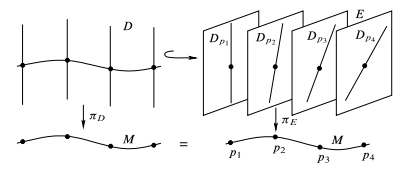
\includegraphics[width=\textwidth]{../\string_build/html/\string_images/subbundle.png}
\caption{Visualisierung eines Untervektorbündels, siehe Kapitel 10 in \cite{Lee03}.}\label{\detokenize{manifolds/diffformen:fig-subbundle}}\end{figure}

\par
In diesem Fall erhält man also ein Untervektorbündel.
\begin{lemma}{}{manifolds/diffformen:lemma-1}



\par
Sei \(\M\) eine glatte \(n\) dimensionale Mannigfaltigkeit, dann ist \(\Lambda^k T^\ast\M\) ein glattes Untervektorbündel vom Rang \(\begin{pmatrix} n k \end{pmatrix}\).
\end{lemma}

\begin{proof}
 ToDo.
\end{proof}

\par
Dank der Bündelstruktur können wir erneut glatte Schnitte betrachten, welche nun auf das Konzept der Differentialform führen.
\begin{definition}{}{manifolds/diffformen:definition-2}



\par
Es sei \(\M\) eine glatte Mannigfaltigkeit, dann nennt man einen glatten Schnitt
\begin{align*}
\omega\in \Gamma(\Lambda^k T^\ast\M)
\end{align*}
\par
eine \(k\) Differentialform oder auch \(k\) Form. Den Vektorraum der Differentialformen notieren wir durch
\begin{align*}
\Omega^k(\M) := \Gamma(\Lambda^k T^\ast\M).
\end{align*}\end{definition}


\subsection{Das äußere Produkt}
\label{\detokenize{manifolds/diffformen:das-auszere-produkt}}
\par
In \hyperref[\detokenize{vektoranalysis/tensor:s-symtensoren}]{Abschnitt \ref{\detokenize{vektoranalysis/tensor:s-symtensoren}}} haben wir das äußere Produkt \(\wedge\) kennengelernt, welches wir nun auf Differentialformen übertragen. Dazu seien \(\omega\in \Omega^k(\M), \eta\in \Omega^l(\M)\) zwei Differentialformen für \(k,l\in\N\), dann setzten wir
\begin{align*}
\omega \wedge \eta:\M &\to \Lambda^{k+l}T^\ast\M\\
p&\mapsto \omega_p \wedge \eta_p
\end{align*}
\par
was in der Tat eine Differentialform definiert, also \(\omega\wedge\eta \in \Omega^{k+l}(\M)\). Zusätzlich überträgt sich auch die Darstellung in einer lokalen Karte von \cref{manifolds/tangential:cor:tensorfieldchart} auf diese Situation, wobei das Tensorprodukt, durch das äußere Produkt ersetzt werden kann.
\begin{lemma}{}{manifolds/diffformen:lemma-3}



\par
Es sei \(\M\) eine glatte Mannigfaltigkeit, \((\varphi,U)\) eine Karte und \(\omega\in\Omega^l(\M)\) eine Differentialform, dann gilt lokal in \(U\)
\begin{align*}
\omega = \sum_{1\leq i_1,\ldots,i_k \leq n}\omega_{i_1\ldots i_k}
dx_{i_1}\wedge\ldots\wedge dx_{i_k},
\end{align*}
\par
wobei \(\omega_{i_1\ldots i_k}\in C^\infty(\M)\) für alle \(i_1,\ldots,i_k\in\{1,\ldots,n\}\) gilts
\end{lemma}

\begin{proof}
 Siehe z.B. \cite{Lee03} Kapitel 14.
\end{proof}
\begin{example}{}{manifolds/diffformen:example-4}



\par
1. Für \(k=0\) und \(\M\) eine glatte Mannigfaltigkeit erhalten wir
\begin{align*}
\Omega^0(\M) = C^\infty(\M).
\end{align*}


\par
2. Für \(k=1\) und \(\M\) eine glatte Mannigfaltigkeit erhalten wir
\begin{align*}
\Omega^1(\M)
\end{align*}
\par
gerade die Kovektorfelder aus \hyperref[\detokenize{manifolds/tangential:s-kotangbundel}]{Abschnitt \ref{\detokenize{manifolds/tangential:s-kotangbundel}}}.



\par
3. Für \(k=3\) und \(\M=\R^3\) ist z.B.,
\begin{align*}
\omega(xy) := \sin(xy) dx\wedge dy
\end{align*}
\par
eine Differentialform.
\end{example}


\subsection{Die äußere Ableitung}
\label{\detokenize{manifolds/diffformen:die-auszere-ableitung}}
\par
Wir wenden uns nun einer wichtigen Operation auf Differentialformen zu, der äußeren Ableitung. Aus \cref{manifolds/tangential:ex:totdiff} kennen wir schon das totale Differential \(df\in \Omega^1(\M)\), für eine glatte Funktion \(f\in C^\infty(\M)\). Hierbei haben wir für ein glattes Vektorfeld \(X\in \Gamma(T\M)\) die Abbildung
\begin{align*}
df(X) := X(f)
\end{align*}
\par
definiert, wobei die rechte Seite über die Wirkung des Vektorfelds definiert ist. Wir können dieses Konzept verallgemeinern, indem wir die äußere Ableitung definieren.
\begin{definition}{}{manifolds/diffformen:definition-5}



\par
Es sei \(\M\) eine glatte Mannigfaltigkeit und \(f\in C^\infty(\M)\), dann definieren wir die lineare Abbildung
\begin{align*}
d:\Omega^k(\M)\to \Omega^{k+1}(\M)\\
d(f\, dx^{i_1}\wedge\ldots\wedge dx^{i_k}):= df \wedge dx^{i_1}\wedge\ldots\wedge dx^{i_k}.
\end{align*}\end{definition}
\begin{remark}{}{manifolds/diffformen:remark-6}



\par
Beachte, dass die obige Abbildung nur jeweils für lokale Koordinaten definiert ist. Wegen der Kartenunabängigkeit führt dies aber auf eine eindeutig definierte Funktion, siehe z.B. \cite{Lee03} Kapitel 14. Da wir \(d\) auf den Elementen \(dx^{i_1}\wedge\ldots\wedge dx^{i_k}\) definiert haben erhalten wir jeweils lokal eine eindeutige lineare Fortsetzung, da jedes \(\omega\in \Omega^k(\M)\) lokal die Darstellung
\begin{align*}
\omega = \sum_{1\leq i_1,\ldots,i_k \leq n}\omega_{i_1\ldots i_k}
dx_{i_1}\wedge\ldots\wedge dx_{i_k}
\end{align*}
\par
hat und somit
\begin{align*}
d\omega &= \sum_{1\leq i_1,\ldots,i_k \leq n} d(\omega_{i_1\ldots i_k}
dx_{i_1}\wedge\ldots\wedge dx_{i_k})\\ 
&= \sum_{1\leq i_1,\ldots,i_k \leq n} d(\omega_{i_1\ldots i_k})\wedge
dx_{i_1}\wedge\ldots\wedge dx_{i_k}
\end{align*}\end{remark}
\begin{example}{}{manifolds/diffformen:ex:10.14}



\par
1. Für \(\omega\in\Omega^0(\R^3)\) ist \(d\omega = \frac{\partial\omega}{\partial x_1}dx_1+
\frac{\partial\omega}{\partial x_2}dx_2+\frac{\partial\omega}{\partial x_3}dx_3\).



\par
2. Für \(\omega = \omega_1dx_1+\omega_2dx_2+\omega_3dx_3\in\Omega^1(\R^3)\) ist
\begin{align*}
d\omega &=& (d\omega_1)\wedge dx_1+(d\omega_2)\wedge dx_2+(d\omega_3)\wedge
dx_3\\
&=& \left(\frac{\partial\omega_2}{\partial x_1}-\frac{\partial\omega_1}{\partial x_2}\right)
dx_1\wedge dx_2+ \left(\frac{\partial\omega_3}{\partial x_2}-\frac{\partial\omega_2}{\partial x_3}\right)
dx_2\wedge dx_3\\
&& + \left(\frac{\partial\omega_1}{\partial x_3}-\frac{\partial\omega_3}{\partial x_1}\right)
dx_3\wedge dx_1.
\end{align*}


\par
3. Für \(\omega = \omega_{12}dx_1\wedge dx_2+\omega_{23}dx_2\wedge dx_3
+\omega_{31}dx_3\wedge dx_1 \in\Omega^2(\R^3)\) ist
\begin{align*}
d\omega = \left(\frac{\partial\omega_{12}}{\partial x_3} + \frac{\partial\omega_{23}}{\partial x_1}
+ \frac{\partial\omega_{31}}{\partial x_2}\right)dx_1\wedge dx_2\wedge dx_3.
\end{align*}


\par
4. Für \(\omega\in\Omega^3(\R^3)\) ist \(d\omega=0\).
\end{example}

\par
Für die äußere Ableitung können wir zusätzlich folgende Eigenschaften zeigen.
\begin{lemma}{}{manifolds/diffformen:lem:outeprop}



\par
Es sei \(\M\) eine glatte Mannigfaltigkeit, dann haben wir folgende Eigenschaften.



\par
1. Für \(f,g\in C^\infty(\M)\) gilt
\begin{align*}
d(fg) = d(f)\,g + f\, d(g).
\end{align*}


\par
2. Für \(\omega\in\Omega^k(\M),\eta\in\Omega^l(\M)\) gilt
\begin{align*}
d(\omega\wedge\eta) = (d\omega)\wedge \eta + (-1)^k \omega\wedge (d\eta).
\end{align*}


\par
3. Es gilt \(d\circ d = 0\).
\end{lemma}
\begin{remark}{}{manifolds/diffformen:remark-9}



\par
Da \(d\) Eigenschaft 2 erfüllt, nennt man \(d\) auch Antiderivation.
\end{remark}

\par
Eine interessante Anwendung finden Differntialformen im sog. Poincaré Lemma. Hierfür benötigen wir folgenden Begriffe
\begin{definition}{}{manifolds/diffformen:def:geschlossenexakt}



\par
Es sei \(\M\) eine glatte Mannigfaltigkeit, eine Differentialform \(v\in\Omega^k(\M)\) heißt
\begin{itemize}
\item {} 
\par
\textbf{geschlossen}, wenn \(dv=0\),

\item {} 
\par
\textbf{exakt}, wenn \(v=d\eta\) für ein \(\eta\in\Omega^{k-1}(\M)\) gilt.

\end{itemize}
\end{definition}

\par
Nach Satz {lem:outer:prop broken reference} sind exakte Differentialformen geschlossen, da für \(v=d\eta\) gilt,
\begin{align*}
dv = d(d\eta) = (d\circ d)\eta = 0.
\end{align*}
\par
Das Poincaré Lemma besagt nun, dass auf sternförmigen offenen Mengen \(U\subseteq \R^n\) auch die Umkehrung gilt.
\begin{lemma}{}{manifolds/diffformen:lemma-11}



\par
Es sei \(U\subset\R^n\) eine offene sternförmige Menge, dann gilt für \(\omega\in \Omega^k(\M)\),
\begin{align*}
\omega\text{ ist geschlossen}\Leftrightarrow \omega\text{ ist exakt.}
\end{align*}\end{lemma}

\begin{proof}
 Siehe z.B. \cite{Lee03} Theorem 11.49.
\end{proof}


\subsection{Der Pullback}
\label{\detokenize{manifolds/diffformen:der-pullback}}
\par
Die letzte Operation die wir in diesem Kapitel betrachten ist der sogenannte \textbf{Pullback}. Hierbei betrachten wir zwei glatte Mannigfaltigkeiten \(\M,\mathcal{N}\) und eine glatte Funktion \(F:M\to\mathcal{N}\). Das Ziel ist es nun eine Differentialform auf \(N\), \(\omega\in\Omega^k(\mathcal{N})\) mithilfe von \(F\) auf eine Differentialform auf \(\M\) zurückzuziehen. Ausgewertet an \(p\in\M\) ergibt eine Differentialform \(\eta\in\Omega^k(\M)\) ein Element aus \(L^k(T_p^\ast\M)\),
\begin{align*}
\eta_p\in \Omega^k(T_p\M) \subset L^k(T_p^\ast\M)
\end{align*}
\par
also eine Linearform, welche auf \(k\) Elemente \(v_1,\ldots,v_k\in T_p^\ast\M\) des Kotangentialraums in \(p\) an \(\M\) wirkt. Haben wir nun a priori \(\omega\in\Omega^k(\mathcal{N})\) gegeben brauchen wir deshalb zunächst eine Methode mit der wir Tangentialvektoren über \(F\) von \(\M\) nach \(\N\) vorschieben können, der sogennante \textbf{Pushforward}.
\begin{definition}{}{manifolds/diffformen:definition-12}



\par
Es seien \(\M,\mathcal{N}\) zwei glatte Mannigfaltigkeiten und \(F\in C^\infty(\M,\mathcal{N})\), dann definieren wir für \(p\in\M\)
\begin{align*}
F_\ast:T_p\M\to T_{F(p)}\mathcal{N}\\
D\mapsto \big[f\mapsto D(f\circ F)]
\end{align*}
\par
den sogenannten \textbf{Pushforward}.
\end{definition}

\par
Da wir nun Tangentialvektoren von \(T_p\M\) auf \(T_{F(p)}\mathcal{N}\) schieben können, sind wir in der Lage damit den Pullback von Kotangentialvektoren zu definieren.
\begin{definition}{}{manifolds/diffformen:definition-13}



\par
Es seien \(\M,\mathcal{N}\) zwei glatte Mannigfaltigkeiten und \(F\in C^\infty(\M,\mathcal{N})\), dann definieren wir für \(p\in\M\)
\begin{align*}
F^\ast: T_{F(p)}^\ast\mathcal{N}\to \big[T^p_\M\mapsto\R\big]\\
v \mapsto \big[D\mapsto v(F_\ast(D)) \big]
\end{align*}
\par
den \textbf{Pullback}
\end{definition}
\begin{remark}{}{manifolds/diffformen:remark-14}



\par
Es gilt insbesondere, dass \(F^\ast v \in T_p^\ast\M\) für jedes \(v\in T_{F(p)}^\ast\mathcal{N}\).
\end{remark}

\par
Dieses Konzept können wir nun auf Formen übertragen in dem wir eine neue Differentialform punktweise an \(p\) definieren am Punkt \(F(p)\). Konkret seien \(v_1,\ldots, v_k\in T_p\M\), dann definiere
\begin{align*}
(F^\ast\omega)_p (v_1,\ldots,v_k) := \omega_F(p)\big(F_\ast(v_1),\ldots,F_\ast(v_k)\big).
\end{align*}
\par
Die so definierte Abbildung bildet tatsächlich zwischen den passenden Räumen ab
\begin{align*}
F^\ast:\Omega^k(\mathcal{N})\to\Omega^k(\mathcal{M})\\
\omega\mapsto \big[ p\mapsto (F^\ast\omega)_p \big].
\end{align*}
\par
Zusätzlich erhält man folgende Eigenschaften.
\begin{lemma}{}{manifolds/diffformen:lem:pullbackprop}



\par
Es seien \(\M,\mathcal{N}\) glatte Mannigfaltigkeiten und \(F\in C^\infty(\M,\mathcal{N})\), dann gilt,
\begin{enumerate}

\item {} 
\par
\(F^\ast\) ist linear,

\item {} 
\par
\(F^\ast(\omega\wedge\eta) = F^\ast(\omega) \wedge F^\ast(\eta)\) für \(\omega,\eta\in\Omega^k(\mathcal{N})\).

\item {} 
\par
Für lokale Koordinaten Kovektorfelder \(dy^1,\ldots,dy^m\) und \(f\in C^\infty(\mathcal{N})\) gilt

\end{enumerate}
\begin{align*}
F^\ast(f dy^{i_1}\wedge\ldots\wedge dy^{i_k}) = (f \circ F) d(y^{i_1}\circ F)\wedge\ldots\wedge d(y^{i_k}\circ F).
\end{align*}\end{lemma}

\begin{proof}
 Für 1. und 2. siehe Hausaufgaben, Für 3. siehe \cite{Lee03} Lemma 14.16.
\end{proof}

\par
Im Falle, dass die Mannigfaltigkeiten gleich dem \(\R^n\) bzw. \(\R^m\) sind, also \(\M=\R^n, \mathcal{N}=\R^m\) können wir den Pullback leicht explizit berechnen. Dazu sei \(F:\R^n\to\R^m\) eine glatte Abbildung, \(x_1,\ldots,x_n\) seien Koordinaten für \(\R^n\) und \(y_1,\ldots,y_m\) seien Koordinaten für \(\R^m\).

\par
Zunächst erkennen wir für den Pushforward, \(F_\ast:T_p\M\to T_{F(p)}\mathcal{N}\) dass für \(p\in\M\) gilt,
\begin{align*}
F_\ast(\partial_{x_i^p}) = \sum_{j=1}^m \partial_i F_j\, \partial_{y_j^{F(p)}}
\end{align*}
\par
wobei \(\partial_i F_j\) die \(i\) te partielle Ableitung (im klassichen Sinne) der \(j\) ten Komponente von \(F\) ist.

\par
Betrachten wir also den Pullback eines Kovektorfeldes \(dy^k\) ausgewertet an einem Tangentialvektor \(D\in T_p\M\)
\begin{align*}
D = \sum_{i=^1}^n dx_i^p(D)\, \partial_{x_i^p}
\end{align*}
\par
erhalten wir unter Ausnutzung der Linearität
\begin{align*}
F^\ast(dy^k)_{p}(D) &= dy^k(F_\ast(D)) = 
dy^k\big(\sum_{i=^1}^n dx_i^p(D)\, F^\ast(\partial_{x_i^p})\big)\\
&=
\sum_{i=^1}^n \sum_{j=1}^m dx_i^p(D)\,\partial_i F_j\, dy^k(\partial_{y_j}^{F(p)}).
\end{align*}
\par
Da die Terme \(dy^k(\partial_{y_j})\) gleich dem Kronecker Delta sind,
\begin{align*}
dy^k(\partial_{y_j}^{F(p)}) = \delta_{kj}
\end{align*}
\par
führt dies auf,
\begin{align*}
F^\ast(dy^k)_{p}(D) =
\sum_{i=1}^n dx_i^p(D)\,\partial_i F_k.
\end{align*}
\par
Für das äußere Produkt von \(l\) verschiedenen Kovektorfeldern \(dy^{k_1},\ldots, dy^{k_l}\) und einer glatten Funktion \(f\in C^\infty(\M)\) gilt mit Eigenschaft 2. von \cref{manifolds/diffformen:lem:pullbackprop} \begin{align*}
F^\ast(f\, dy^{k_1}\wedge\ldots\wedge dy^{k_l})_{p} =
f(F(p))\, F^\ast(dy^{k_1})\wedge\ldots\wedge F^\ast(dy^{k_l}).
\end{align*}
\par
Da wir die Terme \(F^\ast(dy^{k_i})\) berechnen können liefert dies ein einfaches Schema um den Pullback einer Differentialform auf \(\R^m\) zu berechnen.
\begin{example}{}{manifolds/diffformen:example-16}



\par
Es sei \(\omega\in \Omega^3(\R^4)\) eine Differentialform gegeben durch
\begin{align*}
\omega(y_1,y_2,y_3,y_4) = dy_1\wedge dy_2\wedge dy_3 + \cos(y_1)dy_1\wedge dy_2 \wedge dy_4
\end{align*}
\par
und \(F:\R^3\to\R^4\) eine glatte Abbildung gegeben durch
\begin{align*}
F(x_1,x_2,x_3) := (x_1, x_3, \sin(x_2), x_3^2).
\end{align*}
\par
Dann berechnen wir
\begin{align*}
F^\ast(dy_1) &= \sum_{i=1}^3 \,\partial_i F_1 dx_i = dx_1\\
F^\ast(dy_2) &= \sum_{i=1}^3 \,\partial_i F_2 dx_i = dx_3\\
F^\ast(dy_3) &= \sum_{i=1}^3 \,\partial_i F_3 dx_i = \cos(x_2)\,dx_2\\
F^\ast(dy_4) &= \sum_{i=1}^3 \,\partial_i F_4 dx_i = 2x_3\,dx_3\\
\end{align*}
\par
und erhalten damit
\begin{align*}
F^\ast(\omega)_{(x_1,x_2,x_3)} &= F^\ast(dy_1)\wedge F^\ast(dy_2)\wedge F^\ast(dy_3) + 
\cos(F_1(x_1,x_2,x_3)) F^\ast(dy_1)\wedge F^\ast(dy_2)\wedge F^\ast(dy_4)\\
&= dx_1 \wedge dx_3\wedge \cos(x_2)\,dx_2 + \cos(x_1)\, 2x_3\,dx_1\wedge dx_3\wedge dx_3\\
&=  -\cos(x_2)\,dx_1 \wedge dx_2\wedge dx_3.
\end{align*}\end{example}


\chapter{Maß  und Integrationstheorie}
\label{\detokenize{masstheorie/intro_masstheorie:masz-und-integrationstheorie}}\label{\detokenize{masstheorie/intro_masstheorie::doc}}
\par
Im ersten Semester haben wir bereits das \emph{Riemann Integral} zur Berechnung des Flächeninhalts zwischen einer Funktion \(f \colon [a,b] \rightarrow \R\) und der x Achse eingeführt (siehe Kapitel 7 in \cite{Bur20}).
Die grundlegende Idee hierbei war es die x Achse in (unterschiedlich große) Intervalle zu unterteilen und mittels dieser Zerlegung Rechtecke zwischen dem Graphen der Funktion und der x Achse zu konstruieren.
Durch das Produkt der Seitenlängen dieser Rechtecke lässt sich nämlich deren Flächeninhalt leicht berechnen und die Summe all dieser Flächeninhalte approximiert den wahren Flächeninhalt zwischen dem Graphen und \(f\) und der x Achse.
Dieses Vorgehen ist zur Erinnerung nochmal in Abbildung \hyperref[\detokenize{masstheorie/intro_masstheorie:fig-riemann-integral}]{Abb.\@ \ref{\detokenize{masstheorie/intro_masstheorie:fig-riemann-integral}}} illustriert.

\begin{figure}[htbp]
\centering


\noindent\includegraphics[width=\textwidth]{../\string_build/html/\string_images/ober\string_untersummen.png}
\caption{Illustration zweier Approximationen des Riemann Integrals einer Funktion durch den Flächeninhalt von Rechtecken. Die grünen und lila Rechtecke visualisieren die Unter  bzw. Obersummen bezüglich des in rot dargestellten Graphen der Funktion. Quelle: \href{https://de.wikipedia.org/wiki/Riemannsches\_Integral}{Wikipedia; Riemannsches Integral}.}\label{\detokenize{masstheorie/intro_masstheorie:fig-riemann-integral}}\end{figure}

\par
Da wir bisher nur die Integration von eindimensionalen Funktionen auf kompakten Intervallen kennengelernt haben, wollen wir in diesem Kapitel den Begriff des Integals auf mehrdimensionale Funktionen \(f \colon \R^n \rightarrow \R\) erweitern.
Das Riemann Integral lässt sich problemlos auf mehrdimensionalen Funktionen verallgemeinern, indem man das Integral nicht durch den Flächeninhalt von Rechtecken approximiert, sondern hierfür das \emph{Volumen von entsprechenden Quadern} \(Q \subset \R^n\) berechnet.
Es lässt sich insbesondere zeigen, dass jede stetige mehrdimensionale Funktion auf einem (nicht ausgeartetem) Quader Riemann integrierbar ist.

\par
Es hat sich jedoch in der Entwicklung der Mathematik herausgestellt, dass der Begriff des Riemann Integrals zu starke Forderungen an die zu Grunde liegenden Funktionen stellt und damit wichtige und interessante Funktionsklassen nicht integrierbar waren.
Als Beispiel hierfür seien \href{https://de.wikipedia.org/wiki/Fraktal}{fraktale Mengen und Funktionen} genannt, welche auch zur Modellierung von Prozessen in der Natur genutzt werden.

\par
Aus diesem Grund hat sich ein eigenes Feld innerhalb der modernen Analysis gebildet   die sogenannte \textbf{Maßtheorie}.
Es widmet sich hauptsächlich der Untersuchung von Maßen zur Berechnung von Längen, Flächen und Volumina in unterschiedlichen mathematischen Strukturen und Räumen.
Es wird klar, dass Integration und die Berechnung von Volumina eng miteinander zusammen hängen, denn ist \(A\subset\R^n\) eine (messbare) Teilmenge, dann ist ihr Maß gleich dem Integral ihrer charakteristischen Funktion, d.h.,
\begin{align*}
\int_{\R^n} \mathbb{1}_A(x)\,\mathrm{d}x.
\end{align*}
\par
In einem gewissen Sinn sind Maße ein \emph{fundamentaleres Konzept} als das der Integration, da sich jede Integration auf die Berechnung von Maßen stützt.

\par
Eins der berühmtesten Beispiele zur Motivation der Maßtheorie ist im Folgenden erklärt.
\begin{example}{(Dirichlet Funktion)}{masstheorie/intro_masstheorie:ex:dirichletFunktion}



\par
Wir betrachten das kompakte Intervall \([0,1] \subset \R\) und definieren hierauf die sogenannte \textbf{Dirichlet Funktion} \(\mathbb{1}_\Q \colon [0,1] \rightarrow \{0,1\}\) mit
\begin{align*}
\mathbb{1}_\Q(x) := \begin{cases} 1, \ \text{ falls } x \in \Q, \\ 0, \ \text{ sonst }.\end{cases}
\end{align*}
\par
Diese Abbildung kann als \emph{charakteristische Funktion} der rationalen Zahlen \(\Q\) aufgefasst werden.
Man sieht leicht ein, dass diese Funktion \textbf{nicht Riemann integrierbar} ist, da alle Untersummen stets \(0\) und alle Obersummen stets \(1\) sind.
\end{example}

\par
Um eine Funktion wie die Dirichlet Funktion in \cref{masstheorie/intro_masstheorie:ex:dirichletFunktion} zu integrieren sieht man zunächst ein, dass die rationalen Zahlen \(\Q\) in den reellen Zahlen \(\R\) als abzählbare Menge eine sogenannte \emph{Nullmenge} im Sinne der Maßtheorie repräsentieren.
Wir werden im Laufe der Vorlesung die nötigen Werkzeuge der Maßtheorie einführen um diesen Umstand zu verstehen und einen verallgemeinerten Begriff des Integrals definieren, der diese Nullmenge berücksichtigt   das \textbf{Lebesgue Integral}.
Dieses Integral ist eine echte Verallgemeinerung des Riemann Integrals und wir werden einsehen, dass die Menge der Lebesgue integrierbaren Funktionen eine Obermenge der Menge der Riemann integrierbaren Funktionen ist.
Außerdem verhält sich das Lebesgue Integral bei Grenzwertbildungen einfacher als das Riemann Integral.


\section{Maßtheorie}
\label{\detokenize{masstheorie/masstheorie:masztheorie}}\label{\detokenize{masstheorie/masstheorie::doc}}
\par
Wir wollen in diesem Kapitel formal die Maßtheorie einführen, die es uns erlaubt zu entscheiden welche Mengen messbar sind und wie sich das Volumen von Mengen in topologischen Räumen bestimmen lässt.
Die hier beschriebenen Werkzeuge werden uns im nächsten Kapitel bei der Einführung des \emph{Lebesgue Integrals} als Verallgemeinerung des Riemann Integrals sehr dienlich sein.

\par
Intuitiv ordnet ein \href{https://de.wikipedia.org/wiki/Ma\%c3\%9f\_(Mathematik)}{\textbf{Maß}} \(\mu\), welches auf einer Menge \(\Omega\) definiert ist, wie z.B. dem \(\R^n\), allen geeigneten Teilmengen \(A\subseteq \Omega\) nichtnegative reelle Zahlen zu, d.h.
\begin{align*}
\mu(A)\in[0,\infty] := [0,\infty)\cup\{\infty\}.
\end{align*}
\par
Hierbei soll das Maß \(\mu\) natürlich mit dem Volumen der Teilmenge \(A\) zusammenhängen.
Man beachte, dass wir auch explizit unendliche Maße zulassen, z.B., falls die Menge \(\Omega\) schon der gesamte \(\R^n\) ist.

\par
Bevor wir den Begriff des Maßes formal definieren können und dessen Eigenschaften näher diskutieren, müssen wir jedoch noch mehr Verständnis für die zu Grunde liegenden Mengen und Mengensystem entwickeln.


\subsection{\protect\(\sigma\protect\) Algebren und Maße}
\label{\detokenize{masstheorie/masstheorie:sigma-algebren-und-masze}}\label{\detokenize{masstheorie/masstheorie:s-sigmaalg}}
\par
Wir betrachten im Folgenden eine beliebige zu Grundmenge \(\Omega\), welche endlich, abzählbar oder auch überabzählbar sein kann. Ein Maß soll nun Teilmengen von \(\Omega\) einen Wert zuordnen weshalb wir die \textbf{Potenzmenge} \(2^\Omega\) betrachten, welche die Menge aller möglichen Teilmengen von \(\Omega\) bildet. Ein Maß ist dann (unter zusätzlichen Voraussetzungen, siehe \cref{masstheorie/masstheorie:def:mass}  eine spezielle Abbildung \(\mu:\Sigma\to[0,\infty]\), wobei \(\Sigma\subset 2^\Omega\) ein Mengensystem ist, welches man auch System der \(\mu\) messbaren Mengen nennt.

\begin{emphBox}{}{}{Bemerkung:}
\par
Mengen von Mengen nennen wir häufig auch \emph{Mengensysteme}.
\end{emphBox}

\par
Bei der Konstruktion eines Maßes gibt es zwei teilweise konkurrierende Wünsche:
\begin{enumerate}

\item {} 
\par
Möglichst vielen Mengen soll ein Volumen zugeordnet werden können, d.h., \(\Sigma\) soll groß sein.

\item {} 
\par
Das Maß disjunkt vereinigter Mengen soll gleich der Summe der einzelnen Maße sein.

\end{enumerate}

\par
Der erste Wunsch würde darauf hindeuten die Potenzmenge \(2^\Omega\) als System der messbaren Mengen zu betrachten. Allerdings gibt es viele Fälle (siehe \cref{masstheorie/masstheorie:s-vitali} ) in welchen diese Wahl den zweiten Wunsch unmöglich machen. Deshalb ist die Strategie meist ein möglichst großes Teilmengensystem zu finden, s.d. der zweite Wunsch erfüllbar ist. Die Klasse von Systemen auf der wir im Folgenden arbeiten werden, sind sogenannte \(\sigma\) Algebren.
\begin{definition}{(\protect\(\sigma\protect\) Algebra und Messraum)}{masstheorie/masstheorie:def:sigmaalgebra}



\par
Ein Mengensystem \(\Sigma \subseteq 2^\Omega\) heißt \textbf{\(\sigma\) Algebra (von \(\Omega\))}, wenn die folgenden Eigenschaften erfüllt sind
\begin{enumerate}

\item {} 
\par
\(\Omega\in \Sigma\)

\item {} 
\par
\(A\in \Sigma \quad \Rightarrow \quad A^c:=\Omega \setminus A\in \Sigma\)

\item {} 
\par
\((A_n)_{n\in\N} \in \Sigma \quad \Rightarrow \quad \bigcup_{n\in \N} A_n\in \Sigma\).

\end{enumerate}

\par
Für eine \(\sigma\) Algebra \(\Sigma \subseteq \mathcal{P}(\Omega)\) von \(\Omega\) nennen wir das Paar (\(\Omega,\Sigma\)) \textbf{Messraum} und die Mengen des Mengensystems \(\Sigma\) heißen \textbf{messbar}.
\end{definition}

\par
Das Symbol \(\sigma\) erinnert an den Begriff der Summe, insbesondere wegen der dritten Eigenschaft in \cref{masstheorie/masstheorie:def:sigmaalgebra}  also der Abgeschlossenheit unter abzählbarer Vereinigung von Teilmengen.
Aus diesen drei Eigenschaften lässt sich auch direkt zeigen, dass \(\sigma\) Algebren ebenfalls unter \emph{abzählbaren Schnitten} abgeschlossen sind, wie das folgende Lemma zeigt.
\begin{lemma}{(Abgeschlossenheit unter abzählbaren Schnitten)}{masstheorie/masstheorie:lemma-1}



\par
Es sei (\(\Omega,\Sigma\)) ein Messraum und es sei \((A_i)_{i\in_\N}\) eine Familie von Elementen der \(\sigma\) Algebra \(\Sigma\) mit \(A_i \in \Sigma\) für \(i \in \N\).
Dann sind abzählbare Schnitte dieser Mengen auch Elemente der \(\sigma\) Algebra \(\Sigma\), d.h.,
\begin{align*}
\bigcap_{n \in \N} A_n \in \Sigma.
\end{align*}\end{lemma}

\begin{proof}
 Es reicht die Aussage für \(n=2\) zu zeigen. Seien dazu \(A_1,A_2\in\Sigma\), dann folgt \(A_1^C,A_2^C\in\Sigma\) und somit auch \(A^C\cup A_2^C\in\Sigma\). Und somit folgt
\begin{align*}
A_1\cap A_2 = (A_1^C\cup A_2^C)^C \in \Sigma.
\end{align*}\end{proof}

\par
Aus der \cref{masstheorie/masstheorie:def:sigmaalgebra} kann man sich leicht zwei Spezialfälle von \(\sigma\) Algebren überlegen.
Es wird klar, dass das Mengensystem \(\{\emptyset, \Omega\}\) die kleinstmögliche \(\sigma\) Algebra bildet, wohingegen die Potenzmenge \(\mathcal{P}(\Omega)\) die größtmögliche \(\sigma\) Algebra darstellt.

\par
Für ein beliebiges Mengensystem \(\mathcal{C}\subset 2^\Omega\) können wir zusätzlich die erzeugt \(\sigma\) Algebra betrachten, welche die kleinste \(\sigma\) Algebra ist die \(\mathcal{C}\) enthält.
\begin{definition}{(Erzeugte \protect\(\sigma\protect\) Algebra)}{masstheorie/masstheorie:definition-2}



\par
Es sei \(\mathcal{C}\subset 2^\Omega\) ein Mengensystem, dann bezeichnen wir mit
\begin{align*}
\sigma(\mathcal{C}) := \bigcup_{\substack{\Sigma \text{ ist $\sigma$-Algebra}\\ \mathcal{C} \subset \Sigma}} \Sigma
\end{align*}
\par
die von \(\mathcal{C}\) erzeugte \(\sigma\) Algebra.
\end{definition}

\par
Für die erzeugt \(\sigma\) Algebra, haben wir folgende Eigenschaften.
\begin{lemma}{}{masstheorie/masstheorie:lemma-3}



\par
Es sei \(\mathcal{C}\subset 2^\Omega\) ein Mengensystem, dann gilt
\begin{enumerate}

\item {} 
\par
\(\sigma(\mathcal{C})\) ist eine \(\sigma\) Algebra.

\item {} 
\par
\(\sigma(\mathcal{C})\) ist die kleinste \(\sigma\) Algebra die \(\mathcal{C}\) enthält, d.h., falls \(\mathcal{C}\subset\Sigma\) eine weitere \(\sigma\) Algebra ist, so folgt \(\sigma(\mathcal{C})\subset\Sigma\).

\item {} 
\par
Falls \(\mathcal{C}\) selbst eine \(\sigma\) Algebra ist, so folgt \(\sigma(\mathcal{C}) = \mathcal{C}\).

\end{enumerate}
\end{lemma}

\begin{proof}
 Übung.
\end{proof}


\subsection{Maße}
\label{\detokenize{masstheorie/masstheorie:masze}}
\par
Basierend auf dem Begriff einer \(\sigma\) Algebra und eines Messraums können wir nun formal einführen, was wir unter einem Maß verstehen.
\begin{definition}{(Maß und Maßraum)}{masstheorie/masstheorie:def:mass}



\par
Sei \((\Omega, \Sigma)\) ein Messraum.
Wir nennen eine Abbildung \(\mu: \Sigma\to [0, \infty]\) \textbf{Maß}, wenn die folgenden beiden Eigenschaften erfüllt sind.
\begin{enumerate}

\item {} 
\par
Die leere Menge hat das Maß Null, d.h., \(\mu(\emptyset) = 0\),

\item {} 
\par
Für eine Familie von disjunkten Mengen \((A_n)_{n\in\N}\) der \(\sigma\) Algebra \(\Sigma\) mit \(A_i \cap A_j = \emptyset\) für \(i \neq j\) gilt die sogenannte abzählbare oder \(\sigma\) \textbf{Additivität}, d.h.,

\end{enumerate}
\begin{align*}
\mu\left( \bigcup_{n\in\N}A_n \right) = \sum_{n\in\N}\mu (A_n).
\end{align*}
\par
Wir nennen das Maß \(\mu\) \textbf{endlich}, wenn \(\mu(\Omega)<\infty\).
Das Tripel \((\Omega, \Sigma, \mu)\) wird als \textbf{Maßraum} bezeichnet.
\end{definition}
\begin{remark}{}{masstheorie/masstheorie:rem:wahrscheinlichkeitsmass}



\par
Maße spielen insbesondere in der \emph{Wahrscheinlichkeitstheorie} eine zentrale Rolle, um die Wahrscheinlichkeit von Ereignismengen anzugeben.
Dabei wird nicht nur gefordert, dass das Maß \(\mu\) endlich sein muss, sondern dass sogar \(\mu(\Omega)=1\) gilt, damit es sich um ein \textbf{Wahrscheinlichkeitsmaß} handelt.
Diese finden vor allem in der Quantenmechanik Anwendung.
\end{remark}

\par
Aus den beiden grundlegenden Eigenschaften eines Maßes lassen sich weitere nützliche Eigenschaften herleiten, wie das folgende Lemma beschreibt.
\begin{lemma}{(Eigenschaften von Maßen)}{masstheorie/masstheorie:lemma-6}



\par
Sei \((\Omega, \Sigma, \mu)\) ein Maßraum.
Dann gelten die folgenden Eigenschaften für das Maß \(\mu \colon \Sigma \rightarrow [0,\infty]\).

\par
1. Für \(A,B \in \Sigma\) mit \(B \subset A\) und \(\mu(B) < \infty\) gilt:
\begin{align*}
\mu(A \setminus B) = \mu(A) - \mu(B) \qquad \text{(Subtraktivität)}
\end{align*}
\par
2. Für \(A,B \in \Sigma\) mit \(B \subset A\) gilt:
\begin{align*}
\mu(B) \leq \mu(A) \qquad \text{(Monotonie)}
\end{align*}
\par
3. Für \(A,B \in \Sigma\) gilt stets:
\begin{align*}
\mu(A \cup B) = \mu(A) + \mu(B) - \mu(A \cap B).
\end{align*}\end{lemma}

\begin{proof}
 In der Hausaufgabe zu zeigen.
\end{proof}

\par
Im Folgenden wollen wir ein paar Beispiele von geläufigen Maßen diskutieren.
\begin{example}{(Maße)}{masstheorie/masstheorie:example-7}



\par
Wichtige Maße in der Mathematik und Physik sind beispielsweise die folgenden.

\par
1. Das \href{https://de.wikipedia.org/wiki/Z\%c3\%a4hlma\%c3\%9f\_(Ma\%c3\%9ftheorie)}{\textbf{Zählmaß}} \(m\) auf einer \emph{endlichen} Menge \(M\), mit
\begin{align*}
m(A):=|A|\qquad (A\subseteq M).
\end{align*}
\par
Hier sind insbesondere alle Teilmengen messbar, d.h., \((M, \mathcal{P}(M), m)\) bildet einen Maßraum.

\par
2. Das \textbf{Lebesgue–Maß} \(\lambda^n\) auf dem \(\R^n\), das wir bald kennen lernen, zeichnet sich dadurch aus, dass es einer verschobenen Menge das gleiche Volumen zuordnet wie einer unverschobenen.
Es besitzt also die nützliche Eigenschaft \emph{translations } und \emph{rotationsinvariant} zu sein.
Dies gilt ebenfalls für Spiegelungen.
Außerdem ordnet das Lebesgue Maß dem Einheitswürfel \([0,1]^n\) das Maß \(1\) zu, was unserer Intuition entspricht.
Andererseits stellt sich heraus, dass das Lebesgue Maß nicht auf der gesamten Potenzmenge \(\mathcal{P}(\R^n)\) definiert werden kann.

\par
3. Das \href{https://de.wikipedia.org/wiki/Diracma\%c3\%9f}{\textbf{Dirac Maß}} \(\delta_x\) ist im Punkt \(x \in \R^n\) konzentriert, und für jede Teilmenge \(A\subset\R^n\) gilt
\begin{align*}
\delta_x(A) \equiv \int_A\delta_x := \begin{cases} 1, &  \text{ falls } x \in A,\\ 0, & \text{ sonst}. \end{cases}
\end{align*}
\par
Dieses Maß ist im Gegensatz zum Lebesgue Maß nicht translationsinvariant, da es explizit von der Lage des Punkts \(x\in\R^n\) abhängt.
Es wird beispielsweise in der Elektrodynamik benutzt, um eine in \(x\) lokalisierte, punktförmige Ladung zu beschreiben.

\par
4. Häufig möchte man die Länge einer \emph{Kurve} oder allgemeiner den Flächeninhalt einer \(d\) dimensionalen Fläche im \(\R^n\) messen.
Auch das dafür benutzte Maß \(\mu_d\) ist translations  und rotationsinvariant, es ordnet aber der \(d\) dimensionalen Einheitsfläche \([0,1]^d\times\{0\} \subset\R^d\times\R^{n-d}=\R^n\) das Maß \(1\) zu.
Entsprechend hat aber für \(d<n\) der Einheitswürfel das Maß \(\mu_d([0,1]^n)=\infty\).

\par
5. Man kann sogar sogenannte \href{https://de.wikipedia.org/wiki/Hausdorff-Ma\%c3\%9f}{\textbf{Hausdorff Maße}} \(\mu_d\) konstruieren, die Mengen beliebiger fraktaler Dimension \(d\in[0,n]\) messen.
Genau genommen \emph{definiert} man hierbei die Dimension der Menge \(A\subset \R^n\) durch \(d(A):=\inf\{d'>0\mid \mu_{d'}(A)=0\}.\)

\par
6. Im Zusammenhang mit dem sogenannten Feynmanschen \href{https://de.wikipedia.org/wiki/Pfadintegral}{\textbf{Pfadintegral}} der Quantenmechanik wird auf dem unendlich dimensionalen Raum \(\Omega\) der Weg zwischen zwei Punkten des Konfigurationsraumes \(\R^d\) ein \emph{Wahrscheinlichkeitsmaß} (siehe \cref{masstheorie/masstheorie:rem:wahrscheinlichkeitsmass}  definiert.
Dabei erhalten Pfade, die in der Nähe von Lösungskurven der DGL der Klassischen Mechanik sind, ein größeres Gewicht als beliebige Pfade.
\end{example}

\par
Eine sehr nützliche Eigenschaft von gewissen Maßen auf topologischen Räumen ist die der Regularität, welche wir im Folgenden definieren wollen.
\begin{definition}{(Regularität von Maßen)}{masstheorie/masstheorie:def:regularitaet}



\par
Es sei \((\Omega, \tau)\) ein topologischer Raum und \((\Omega, \Sigma, \mu)\) ein entsprechender Maßraum auf \(\Omega\), so dass gilt \(\tau \subset \Sigma\).
Dann können wir die Regulariät des Maßes \(\mu\) wie folgt definieren.
\begin{enumerate}

\item {} 
\par
Wir nennen das Maß \(\mu\) von \textbf{außen regulär}, wenn zu jeder messbaren Menge \(A \in \Sigma\) und jedem \(\epsilon > 0\) eine offene Obermenge \(U \in \tau\) existiert mit \(A \subset U\), so dass für das Maß \(\mu(U\setminus A) < \epsilon\) gilt.

\item {} 
\par
Wir nennen das Maß \(\mu\) von \textbf{innen regulär}, wenn zu jeder messbaren Menge \(A \in \Sigma\) und jedem \(\epsilon > 0\) eine abgeschlossene Teilmenge \(F \subset A\) gibt, so dass für das Maß \(\mu(A\setminus F) < \epsilon\) gilt.

\end{enumerate}
\end{definition}


\subsection{Borel Maße}
\label{\detokenize{masstheorie/masstheorie:borel-masze}}
\par
Neben \(\sigma\) Algebren kennen wir auch Topologien als wichtige Klasse von Mengensystemen, da diese es z.B. erlauben Stetigkeit von Funktionen zu definieren. Wir betrachten nun ein Konzept welches den Begriff einer Topologie mit der einer \(\sigma\) Algebra vereint, die sogenannte \textbf{Borel} \(\sigma\) Algebra.

\begin{emphBox}{}{}

\par
\href{https://de.wikipedia.org/wiki/\%C3\%89mile\_Borel}{Émile Borel} (geboren am 7. Januar 1871 in Saint Affrique; gestorben am 3. Februar 1956 in Paris) war ein französischer Mathematiker und Politiker.
\end{emphBox}
\begin{definition}{(Borel \protect\(\sigma\protect\) Algebra)}{masstheorie/masstheorie:definition-9}



\par
Die \textbf{Borel \(\sigma\) Algebra} auf einem topologischen Raum \((\Omega, \tau)\) ist die von \(\tau\) erzeugte \(\sigma\) Algebra,
\begin{align*}
\B(\Omega) := \sigma(\tau).
\end{align*}\end{definition}
\begin{remark}{(Borelsche \protect\(\sigma\protect\) Algebra von \protect\(\R\protect\))}{masstheorie/masstheorie:remark-10}



\par
Wir bemerken, dass die Borelsche \(\sigma\) Algebra von \(\R\) \textbf{nicht} alle Teilmengen von \(\R\) enthält.
Es lässt sich sogar zeigen, dass die borelsche \(\sigma\) Algebra von \(\R\) gleichmächtig zu \(\R\) ist, während die Potenzmenge \(2^\R\) eine echt größere Mächtigkeit als \(\R\) besitzt.
\end{remark}

\par
Man erkennt an der Notaion, dass die Topologie \(\tau\) meist unterschlagen wird. Man spricht meist auch vom topologischen Raum \(\Omega\) ohne \(\tau\) zu nennen.
Ein Maß auf dieser \(\sigma\) Algebra nennen wir auch \textbf{Borel Maß}.
\begin{definition}{}{masstheorie/masstheorie:definition-11}



\par
Es sei \(\Omega\) ein topologischer Raum, dann heißt ein Maß \(\mu\) auf \(\B(\Omega)\) Borel Maß.
\end{definition}


\subsubsection{Erzeugte Topologien}
\label{\detokenize{masstheorie/masstheorie:erzeugte-topologien}}\label{\detokenize{masstheorie/masstheorie:s-gentop}}
\par
Das Konzept der erzeugten \(\sigma\) Algebra lässt sich auch auf Topologien übertragen. Hierbei betrachtet man meist eine sogenannte Basis einer Topologie.
\begin{definition}{}{masstheorie/masstheorie:definition-12}



\par
Es sei \((\Omega,\tau)\) ein topologischer Raum, ein System \(\mathcal{C}\subset 2^\Omega\) heißt Basis für \(\tau\), falls für jede Menge \(U\in\tau\) Teilmengen aus \(\mathcal{C}\) existieren, \(J\subset\mathcal{C}\), s.d.,
\begin{align*}
\bigcup_{A\in J} A = U.
\end{align*}
\par
In diesem Fall schreiben wir auch \(\tau(\mathcal{C})=\tau\).
\end{definition}

\par
Besonders relevant sind für uns die Mengensysteme, welche die kanonische Topologie für \(\R\) erzeugt. Hierbei wissen wir, dass alle offene \emph{Intervalle} der Form \((a,b)\subset \R\), sowie alle Intervalle der Form \((-\infty, b)\) und \((a, \infty)\) die euklidische Topologie in \(\R\) erzeugen. Wir betrachten weiterhin ein derartiges Mengenssystem bestehend aus Intervallen, welche die Borel \(\sigma\) Algebra erzeugt.
\begin{lemma}{}{masstheorie/masstheorie:lem:genborel}



\par
Es sei
\begin{align*}
\mathcal{C} = \{ [-\infty, c):c\in\R\}
\end{align*}
\par
dann gilt \(\sigma(\mathcal{C}) = \B(\overline{\R})\).
\end{lemma}


\subsubsection{Eigenschaften von Borel Maßen}
\label{\detokenize{masstheorie/masstheorie:eigenschaften-von-borel-maszen}}
\par
Für spezielle topologische Räume lässt sich eine wichtige Eigenschaft von Maßen über die Borel \(\sigma\) Algebra definieren.
\begin{definition}{(Lokale Endlichkeit von Maßen)}{masstheorie/masstheorie:definition-14}



\par
Sei \((\Omega, \tau)\) ein Haussdorf Raum (siehe \cref{manifolds/manifolds_prelim:def:hausdorffraum}  und sei \(\B(\Omega) = \sigma(\tau)\) die Borel \(\sigma\) Algebra, die durch \(\tau\) erzeugt wird.
Wir nennen ein Maß \(\sigma \colon \B(\Omega) \rightarrow [0, \infty]\) \textbf{lokal endlich}, falls jeder Punkt \(x \in \Omega\) eine lokale Umgebung mit endlichem Maß besitzt.
\end{definition}

\par
Die lokale Endlichkeit ist essentiell bei der Untersuchung von Maßen auf topologischen Räumen, weil sie für jeden Punkt die Existenz einer Umgebung mit endlichem Maß garantiert.
Wie wir später sehen werden ist das Lebesgue Maß auf dem Raum \(\R^n\) lokal endlich.

\par
Basierend auf der oben definierten Borel \(\sigma\) Algebra lässt sich nun das sogenannte Borel Maß einführen.
\begin{definition}{(Borel Maß)}{masstheorie/masstheorie:definition-15}



\par
Ein lokal endliches Maß \(\sigma \colon \B(\Omega) \rightarrow [0, \infty]\) auf der Borelschen \(\sigma\) Algebra eines Hausdorff Raums \((\Omega,\tau)\) heißt \textbf{Borel Maß}.
\end{definition}


\subsection{Das Lebesgue Maß}
\label{\detokenize{masstheorie/masstheorie:das-lebesgue-masz}}\label{\detokenize{masstheorie/masstheorie:s-lebesguemeasure}}
\begin{emphBox}{Henri Lebesgue}{}

\par
\href{https://en.wikipedia.org/wiki/Henri\_Lebesgue}{Henri Léon Lebesgue} (Geboren 28. Juni 1875 in Beauvais; Gestorben 26. Juli 1941 in Paris) war ein französischer Mathematiker.
\end{emphBox}

\par
Bei der Einführung des Riemann Integrals verwendet man Intervalle zur Unterteilung des Definitionsbereichs.
Diese Partitionierung einer Menge lässt sich im \(\R^n\) auf mehrdimensionale Quader verallgemeinern. Für \(a = (a_1,\ldots,a_n) \in \R^n\) und \(b = (b_1,\ldots,b_n) \in \R^n\) verwenden wir hierbei die Anordnungsrelation
\begin{align*}
a < b \qquad \Leftrightarrow \qquad a_i < b_i \quad i=1,\ldots,n
\end{align*}
\par
und analog für \(a \leq b, a > b\) und \(a \geq b\).
\begin{definition}{}{masstheorie/masstheorie:def:quader}



\par
und darüber im Folgenden \textbf{offene, halboffene} und \textbf{abgeschlossene Quader} im \(\R^n\) respektive beschreiben durch
\begin{align*}
(a,b) &= \lbrace x \in \R^n : a < x < b \rbrace,\\
(a,b] &= \lbrace x \in \R^n : a < x \leq b \rbrace,\\
[a,b] &= \lbrace x \in \R^n : a \leq x \leq b \rbrace.
\end{align*}
\par
Das \textbf{Volumen} bzw. der Lebesgue Inhalt eines halboffenen Quaders \(Q := (a,b] \subset \R^n\) definieren wir über
\begin{align*}
\lambda^n(Q) := \prod_{i=1}^n (b_i - a_i).
\end{align*}\end{definition}

\par
Wir wollen im Folgenden das Teilmengensystem \(\mathcal{R}_{\text{Q}}\subset\ 2^{\R^n}\) aller halboffenen Quader betrachten,
\begin{align*}
\mathcal{R}_{\text{Q}} := \left\{ \bigsqcup_{i=1,\ldots,k} Q_i \colon Q_i \text{ ist halboffener Quader im } \R^n \right\}.
\end{align*}
\par
Wir fordern hierbei nicht, dass nur disjunkte Quader vereinigt werden dürfen. Jedoch kann man direkt herleiten, dass man jede Vereinigung von Quadern in eine disjunkte Umschreiben kann. Seien dazu \(Q_1,\ldots,Q_k\subset\R^n\) halboffene Quader, wir erkennen, dass der Rand eines Quaders \(Q_i=(a^i,b^i]\) genau \(2n\) Hyperebenen der Form
\begin{align*}
x_j = a^i_j\\
x_j = b^i_j
\end{align*}
\par
für \(j=1,\ldots,n\) aufspannt. Weiterhin, können wir einen anderen Quader \(Q_m=(a^k,b^k)\) mit einer Hyperebene \(x_l=c\in\R\) zerteilen, im Falle \(a^k_l < c < b^k_l\), indem wir zwei neue Quader definieren mit
\begin{align*}
\alpha^m&:=(a^m_1,\ldots,c,\ldots,a^m_n)\\
\beta^m&:=(b^m_1,\ldots,c,\ldots,b^m_n)\\
Q_m^1&=(a^m,\beta^m]\\
Q_m^2&=(\alpha^m,b^m].
\end{align*}
\par
Iterativ gehen wir folgendermaßen vor:
\begin{enumerate}

\item {} 
\par
Betrachte den ersten Quader \(Q_1\), zerteile alle Quader \(Q_i\) an allen seinen Hyperebenen und erhalte so neue Quader \(W^1_j\).

\item {} 
\par
Im \(i+1\)ten Schritt betrachte die Hyperebenen des Quaders \(Q_{i+1}\) und zerteile damit alle Quader \(W^i_j\) aus dem vorherigen Schritt und erhalte damit neue Quader \(W^{i+1}_j\).

\end{enumerate}

\par
Führen wir diesen Prozess bis \(i=k\) durch, so erhalten wir folgendes Resultat, welches in \hyperref[\detokenize{masstheorie/masstheorie:fig-disrect}]{Abb.\@ \ref{\detokenize{masstheorie/masstheorie:fig-disrect}}} visualisiert ist.

\begin{figure}[htbp]
\centering


\noindent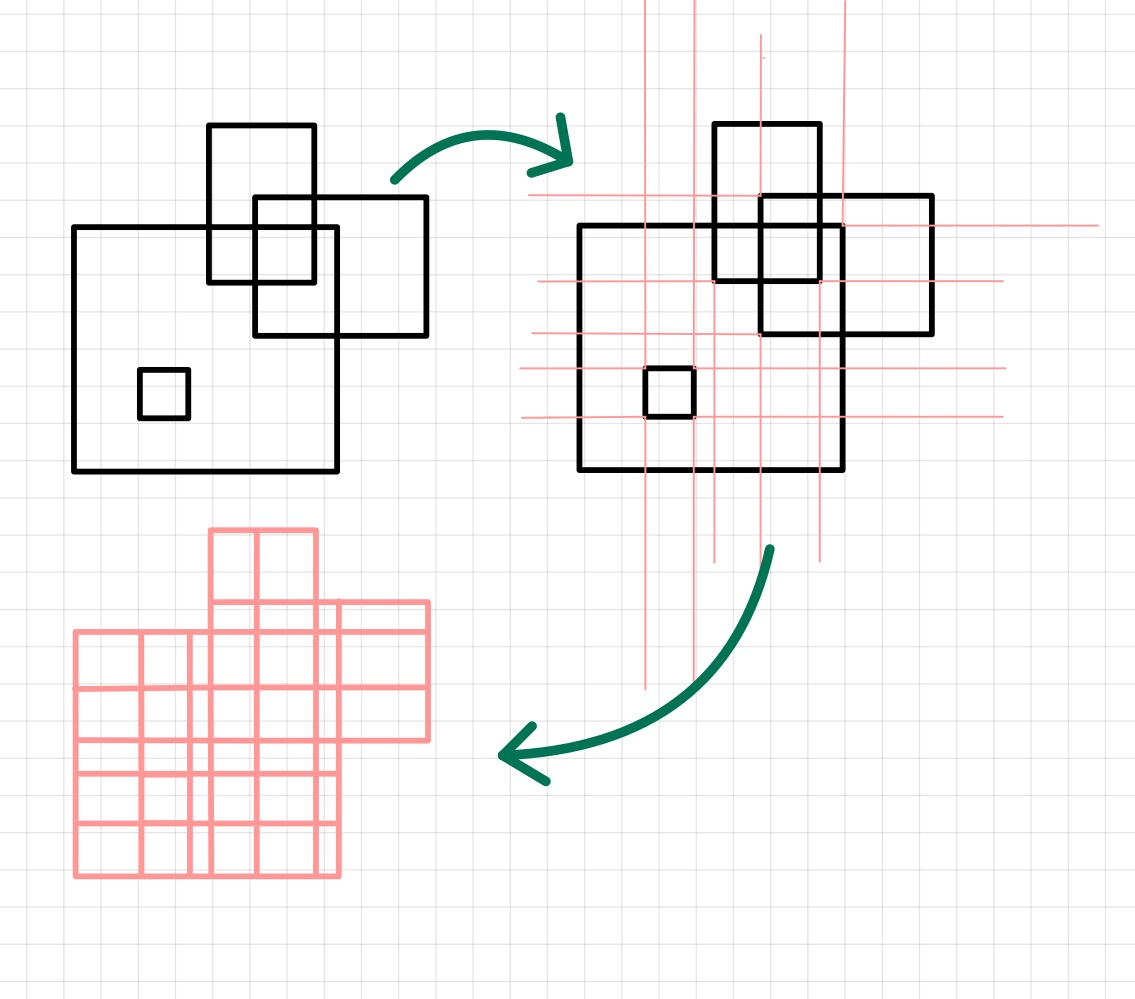
\includegraphics[width=\textwidth]{../\string_build/html/\string_images/DisRect.jpg}
\caption{Nicht disjunkte Quader werden in System disjunkter Quader überführt. Man erkennt insbesondere, dass die Vereinigung gleich bleibt und, dass sich jeder einzelne ursprüngliche Quader, aus den neuen Quadern zusammensetzbar ist.}\label{\detokenize{masstheorie/masstheorie:fig-disrect}}\end{figure}
\begin{lemma}{}{masstheorie/masstheorie:lem:disRect}



\par
Es seien \(Q_1,\ldots,Q_k\subset\R^d\) halboffene Quader, dann existieren paarweise disjunkte halboffene Quader \(W_1,\ldots, W_M\) mit Indexmengen \(J_i\subset\{1,\ldots,M\}\), s.d.
\begin{align*}
\bigcup_{i=1}^k Q_i = \bigcup_{j=^1}^M W_j
\end{align*}
\par
und für jedes \(i\in\{1,\ldots,n\}\) gilt
\begin{align*}
\bigcup_{j\in J_i} W_j = Q_i.
\end{align*}\end{lemma}

\par
Das System der halboffenen Quadern bildet eine besondere mathematische Struktur, einen sogenannten Mengen Ring.
\begin{definition}{}{masstheorie/masstheorie:def:ring}



\par
Ein Mengensystem \(\mathcal{R} \subset 2^{\Omega}\) heißt \textbf{Mengen Ring} (im maßtheoretischen Sinne) auf einer Menge \(\Omega\), falls die folgenden Eigenschaften erfüllt sind:
\begin{enumerate}

\item {} 
\par
\(\emptyset \in \mathcal{R}\)

\item {} 
\par
\(A,B \in \mathcal{R} \Rightarrow (A \setminus B) \in \mathcal{R}\)

\item {} 
\par
\(A,B \in \mathcal{R} \Rightarrow (A \cup B) \in \mathcal{R}\)

\end{enumerate}
\end{definition}
\begin{lemma}{(Der von halboffenen Quadern erzeugte Ring)}{masstheorie/masstheorie:lemma-19}



\par
Das System der halboffenen Quadern \(\mathcal{R}_{\text{Q}}\) bildet einen Mengenring.
\end{lemma}

\begin{proof}
 Um zu zeigen, dass es sich bei dem Mengensystem \(\mathcal{R}_{\text{Q}}\) um einen Ring handelt müssen wir die Eigenschaften aus \cref{masstheorie/masstheorie:def:ring} nachweisen.

\par
1. Für einen beliebigen Punkt \(a \in \R^n\) gilt \(\emptyset = (a,a] \in \mathcal{R}_{\text{Q}}\).

\par
2. Als nächstes müssen wir zeigen, dass für zwei Mengen \(A,B \in \mathcal{R}_{\text{Q}}\) gilt, dass auch die Mengendifferenz in \(\mathcal{R}_{\text{Q}}\) enthalten ist, d.h., dass gilt \((A \setminus B) \in \mathcal{R}_{\text{Q}}\). Nach \{prf:ref\}``disRect` existieren paarweise disjunkte halboffene Quader \(S_j\), \(j=1,\ldots,n\), und Indexmengen \(I_A,I_B\subset\{1,\ldots,n\}\), s.d.,
\begin{align*}
A = \bigcup_{j\in I_A} S_j\\
B = \bigcup_{j\in I_B} S_j.
\end{align*}
\par
Somit gilt dann
\begin{align*}
A\setminus B &= \left(\bigcup_{j\in I_A} S_j\right) \setminus \left(\bigcup_{j\in I_B} S_j\right)\\ 
&= \bigcup_{j\in I_A\setminus I_B} S_j
\end{align*}
\par
was wieder eine Vereinigung von halboffenen Quadern ist und deshalb gilt \(A\setminus B\in \mathcal{R}_{\text{Q}}\).

\par
3. Zuletzt erkennen wir für zwei Mengen \(A,B \in \mathcal{R}_{\text{Q}}\), dass mit der Zerlegung aus 2. gilt
\begin{align*}
A\cup B = \bigcup_{j=1}^n S_j
\end{align*}
\par
und somit ist auch \(A\cup B\in\mathcal{R}_{\text{Q}}\) als Vereinigung halboffener Quader.

\par
Damit haben wir gezeigt, dass das Mengensystem \(\mathcal{R}_{\text{Q}}\), welches durch disjunkte halboffene Quader im \(\R^n\) erzeugt wird, einen Ring bildet.
\end{proof}

\par
Wir können den Lebesgue Inhalt nun auf Elemente von \(\mathcal{R}_{\text{Q}}\) fortsetzen
\begin{definition}{}{masstheorie/masstheorie:definition-20}



\par
Es sei \(A\in\mathcal{R}_{\text{Q}}\) mit \(A=\bigcup_{i=1}^n Q_i\) wobei \(Q_1,\ldots,Q_n\) \textbf{paarweise disjunkte} halboffene Quader sind, dann setzen wir
\begin{align*}
\lambda^n(A):=\sum_{i=1}^{n} \lambda^n(Q_i).
\end{align*}\end{definition}
\begin{remark}{}{masstheorie/masstheorie:remark-21}



\par
Man erkennt leicht, dass der Wert \(\lambda^n(A)\) \textbf{nicht} von der Wahl der Zerlegung \(Q_1,\ldots,Q_n\) abhängt, der Lebesgue Inhalt ist also wohldefiniert.
\end{remark}

\par
Für den Lebesgue Inhalt auf \(\mathcal{R}\) können wir folgende Eigenschaften zeigen.
\begin{theorem}{}{masstheorie/masstheorie:thm:lebesguevolume}



\par
Der Lebesgue Inhalt \(\lambda^n\) auf \(\mathcal{R}\) hat folgende Eigenschaften:

\par
1. \(\lambda^n(\emptyset) = 0\)

\par
2. Seien \(A_1, \ldots, A_k \in \mathcal{R}\) disjunkte Mengen.
Dann gilt:
\begin{align*}
\lambda^n \left( \bigcup_{i=1,\ldots,k} A_i \right) = \sum_{i=1}^k \lambda^n(A_i) \qquad (\text{endliche Additivität})
\end{align*}
\par
3. Für zwei Mengen \(A, B \in \mathcal{R}\) mit \(A \subset B\) gilt:
\begin{align*}
\lambda^n(A) \leq \lambda^n(B) \qquad (\text{Monotonie}).
\end{align*}
\par
4. Für zwei Mengen \(A, B \in \mathcal{R}\) gilt:
\begin{align*}
\lambda^n(A \cup B) + \lambda^n(A \cap B) = \lambda^n(A) + \lambda^n(B).
\end{align*}
\par
5. Für beliebige Mengen \(A_1, \ldots, A_k \in \mathcal{R}\) gilt:
\begin{align*}
\lambda^n\left( \bigcup_{i=1,\ldots,k} A_i\right) \leq \sum_{i=1}^k \lambda^n(A_i) \qquad (\text{endliche Subadditivität}).
\end{align*}
\par
6. Sei \((A_n)_{k\in\N}\) eine Folge von disjunkten Mengen in \(\mathcal{R}\) und sei \(B \in \mathcal{R}\), so dass \(\bigcup_{k=1}^\infty A_k \subset B\), dann gilt
\begin{align*}
\sum_{k=1}^\infty  \lambda^n(A_k) \leq \mu(B).
\end{align*}\end{theorem}

\begin{proof}
 \textbf{Ad 1.}

\par
Für \(a\in\R^d\) haben wir
\begin{align*}
\lambda^n(\emptyset) = \lambda^n((a,a]) = \Pi_{i=1}^n (a_i - a_i) = 0.
\end{align*}
\par
\textbf{Ad 2.}

\par
Für disjunkte Mengen \(A_1,\ldots, A_k\in\mathcal{R}\) wählen wir für jedes \(i\in\{1,\ldots,k\}\) paarweise disjunkte Quader
\(Q^i_1,\ldots, Q^i_{n_i}\), welche nach \cref{masstheorie/masstheorie:lem:disRect} existieren, s.d.,
\begin{align*}
A_i = \bigcup_{j=1}^{n_i} Q^i_j.
\end{align*}
\par
Da die \(A_i\) paarweise disjunkt sind, gilt insbesondere
\begin{align*}
Q^i_j \cap Q^r_s = \emptyset
\end{align*}
\par
für \((i,j)\neq (r,s)\). Somit haben wir
\begin{align*}
\lambda^n\left(\bigcup_{i=1}^k A_i \right) &= \lambda^n\left(\bigcup_{i=1}^k \bigcup_{j=1}^{n_i} Q^i_j \right) 
\\&=
\sum_{i=1}^k \sum_{j=1}^{n_i} \lambda^n(Q^i_j)
\\&= 
\sum_{i=1}^k \lambda^n(A_i).
\end{align*}
\par
\textbf{Ad 3.}

\par
Es sei \(A\subset B\), dann können wir \(B\) disjunkt zerlegen mit
\begin{align*}
B = A \cup B\setminus A
\end{align*}
\par
und sehen dann unter Ausnutzung von 2.
\begin{align*}
\lambda^n(B) = \lambda^n((A\cap B)\cup B\setminus B) \overset{2.}{=} 
\lambda^n(A) + \underbrace{\lambda(B\setminus A)}_{\geq 0} \geq \lambda^n(A).
\end{align*}
\par
\textbf{Ad 4.}

\par
Für zwei Mengen \(A,B\in\mathcal{R}_{\text{Q}}\) sehen wir, dass
\begin{align*}
A\cup B = A \cup (B\setminus A),
\end{align*}
\par
gilt, wobei die Mengen auf der rechten Seite paarweise disjunkt sind. Mit 2. haben wir dann
\begin{align*}
\lambda^n(A\cup B) + \lambda^n(A\cap B)
&= \lambda^n(A) + \lambda^n(B\setminus A) + \lambda^n(A\cap B)
\\&= 
\lambda^n(A) + \lambda^n(B).
\end{align*}
\par
\textbf{Ad 5.}

\par
Nach 4. gilt für zwei Mengen \(A,B\in\mathcal{R}\),
\begin{align*}
\lambda^n(A\cup B) = \lambda^n(A) + \lambda^n(B) - \lambda^n(A\cap B) \leq \lambda^n(A) + \lambda^n(B).
\end{align*}
\par
Diese Eigenschaft lässt sich direkt auf endliche viele Mengen \(A_1,\ldots,A_k\in\mathcal{R}\) übertragen.

\par
\textbf{Ad 6.}

\par
Es sei \((A_i)_{i\in\N}\subset \mathcal{R}_{\text{Q}}\) eine Folge paarweiser disjunkter Mengen, s.d.,
\begin{align*}
\bigcup_{i\in\N} A_i\subset B\in \mathcal{R}_{\text{Q}}.
\end{align*}
\par
Dann gilt für \(N\in\N\)
\begin{align*}
\sum_{i=1}^N \lambda^n(A_i) 
\overset{2.}{=} \lambda^n\left(\bigcup_{i=1}^N\right) 
\overset{3.}{\leq} \lambda^n\left(\bigcup_{i=1}^\infty\right)
\overset{3.}{\leq} \lambda^n(B).
\end{align*}
\par
Somit gilt mit \(N\to\infty\)
\begin{align*}
\sum_{i=1}^\infty \lambda^n(A_i) \leq \lambda^n(B).
\end{align*}\end{proof}


\subsubsection{Der Jordan Inhalt und Jordan messbare Mengen}
\label{\detokenize{masstheorie/masstheorie:der-jordan-inhalt-und-jordan-messbare-mengen}}
\par
Wir haben bisher einen Inhalt auf \(\mathcal{R}_{\text{R}}\) definiert. Diese Klasse an Mengen ist aber relativ klein, weshalb der Begriff ausgedehnt werden soll. Eine Möglichkeit hier ist die Idee des Riemann Integrals mit Ober  und Untersummen zu benutzen. Es stellt aber auch hier heraus, dass der Begriff zu einschränkend ist. Insbesondere führt deses Konzept \textbf{nicht} auf ein Maß. Wir werden es im Folgenden trotzdem betrachten.
\begin{definition}{}{masstheorie/masstheorie:definition-23}



\par
Sei \(A \subset \R^n\) eine beliebige Teilmenge.
Wir betrachten die folgenden \textbf{endlichen} Ober  und Untersummen für die Teilmenge \(A\),
\begin{align*}
\iota^\ast(A) &:= \inf \left\{ \lambda^n(O) \, : A \subset O \in\mathcal{R}_{\text{R}}\right\},\\
\iota_\ast(A) &:= \sup \left\{ \lambda^n(U \, : A \supset U\in\mathcal{R}_{\text{R}} \right\}.
\end{align*}
\par
Wir nennen die Teilmenge \(A \subset \R^n\) \textbf{Jordan messbar}, genau dann wenn \(A\) beschränkt ist und die Ober  und Untersumme übereinstimmen, d.h., es gilt \(\iota^\ast(A) = \iota_\ast(A)\).
Für Jordan messbare Mengen \(A\) ist dann der Jordan Inhalt \(\iota\) gegeben durch:
\begin{align*}
\iota(A) = \iota^\ast(A) = \iota_\ast(A).
\end{align*}\end{definition}

\begin{figure}[htbp]
\centering


\noindent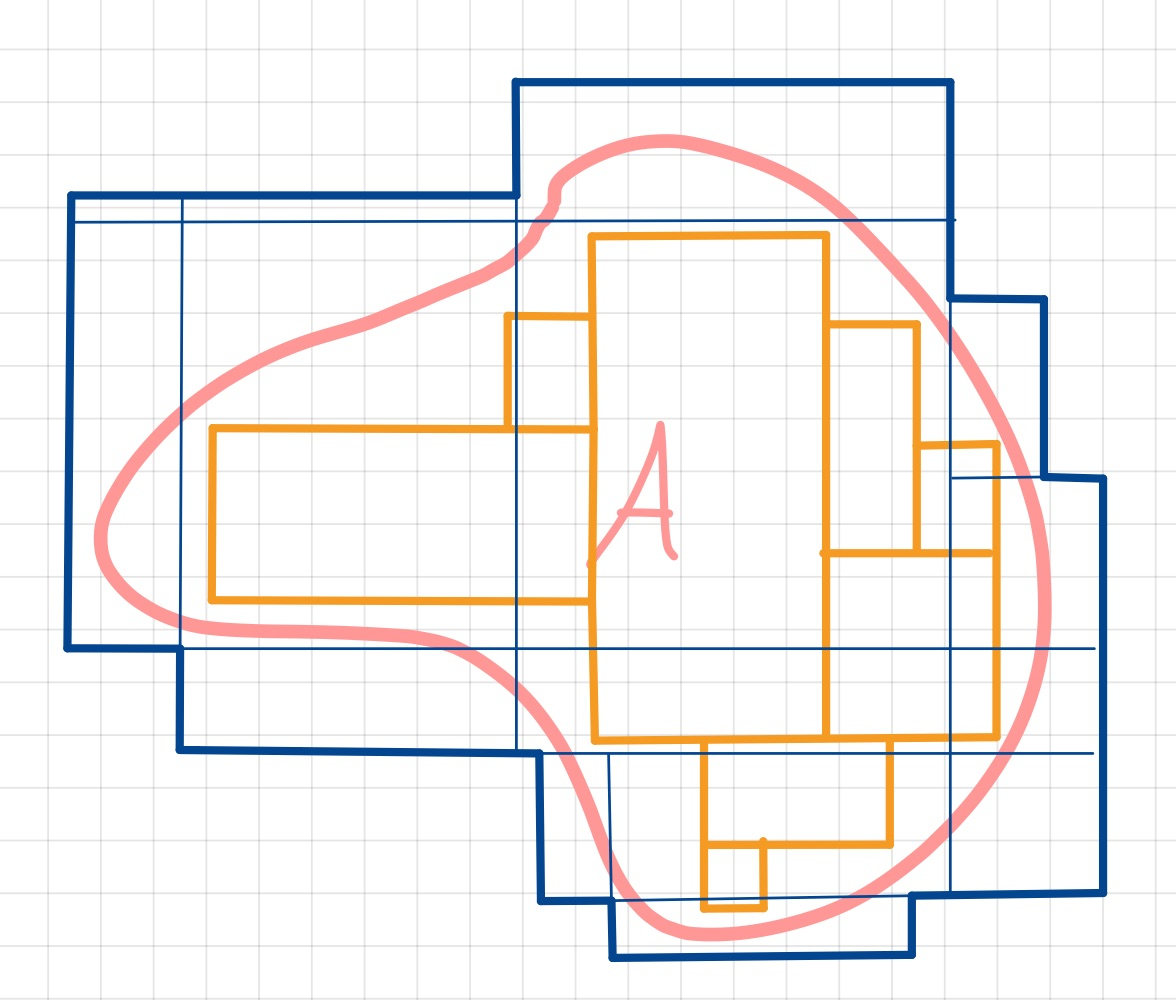
\includegraphics[width=\textwidth]{../\string_build/html/\string_images/jordanmeasure.jpg}
\caption{Visualisierung einer Approximation für das äußere (blau) und das inner (orange) Maß.}\label{\detokenize{masstheorie/masstheorie:fig-jordanmeasure}}\end{figure}

\par
Die Klasse der Jordan messbaren Mengen ist erneut recht klein. Insbesondere hat dieses Konzept erneut Schwierigkeiten mit abzählbar unendlich großen Mengen umzugehen wie folgendes Beispiel zeigt.
\begin{example}{}{masstheorie/masstheorie:ex:jordan}



\par
Wir betrachten die Menge
\begin{align*}
A = (0,1]\cap \mathbb{Q}
\end{align*}
\par
der rationalen Zahlen im Intervall \([0,1]\). Wir betrachten zunächst das äußere Maß und dazu eine Menge
\begin{align*}
J = \bigcup_{i=1}^N Q_i \supset A,
\end{align*}
\par
mit halboffenen Quader \(Q_1,\ldots,Q_N\). Da aber \(J\) und \((0,1]\) jeweils Elemente aus \(\mathcal{R}_{\text{Q}}\) sind gilt auch
\(L = (0,1]\setminus J \in\mathcal{R}\). Wäre nun \(L\) nicht leer, so gäbe es per Definition der halboffenen Quader eine offene Umgebung
\begin{align*}
U\subset L.
\end{align*}
\par
Da aber \(A\) dicht in \((0,1]\) liegt und somit auch \(J\) führt dies auf einen Widerspruch. Deshalb folgt \(L=\emptyset\) und daher
\begin{align*}
(0,1]\subset J \Rightarrow 1\leq \iota^\ast(A).
\end{align*}
\par
Für das innere Maß betrachten wir
\begin{align*}
J = \bigcup_{i=1}^N Q_i \subset A,
\end{align*}
\par
angenommen \(J\) wäre nicht leer, dann folgt dass eine offenen Umgebung \(U\) existiert s.d.
\begin{align*}
U\subset J.
\end{align*}
\par
Da aber auch die irrationalen Zahlen \(\R\setminus \mathbb{Q}\) dicht in \(\R\) liegen folgt daher
\begin{align*}
\left[U\cap\R\setminus \mathbb{Q} \neq \emptyset\right] 
\Rightarrow 
\left[J \cap \R\setminus \mathbb{Q} \neq \emptyset\right]
\Rightarrow 
\left[J\not\subset \mathbb{Q}\right]
\end{align*}
\par
was im Widerspruch zu \(J\subset A\) steht, daher gilt
\begin{align*}
J=\emptyset\Rightarrow \iota_\ast(J) = 0
\end{align*}
\par
und somit
\begin{align*}
\iota_\ast(J) \neq \iota^\ast(J).
\end{align*}\end{example}

\par
Die Menge der Jordan messbaren Mengen bildet weiterhin keine \(\sigma\) Algebra und daher ist der Jordan Inhalt kein Maß im Sinne von \cref{masstheorie/masstheorie:def:mass}  Dies ist an folgendem Beispiel ersichtlich.
\begin{example}{}{masstheorie/masstheorie:example-25}



\par
Wir wollen den Jordan Inhalt einer Punktmengen \(\{a\}\) für \(a\in\R\) berechnen. Mit der Argumentation aus \cref{masstheorie/masstheorie:ex:jordan} erkennen wir, dass das innere Maß gleich null ist, also
\begin{align*}
\iota_\ast(\{a\}) = 0.
\end{align*}
\par
Für das äußere Maß wählen wir eine Folge von offenen Quadern \(Q_i:= (a-1/i, a] \supset \{a\}\) und erkennen, dass
\begin{align*}
\iota^\ast(\{a\})\leq \lim_{i\to\infty} \lambda^n(Q_i) = \lim_{i\to\infty} 1/i = 0
\end{align*}
\par
und damit ist jede Punktmenge Jordan messbar.

\par
Da aber \(\mathbb{Q}\) abzählbar ist, können wir eine Folge \((q_i)_{i\in\N}\) finden, s.d.
\begin{align*}
A = (0,1]\cap \mathbb{Q} = \bigcup_{i\in\N} \{q_i\},
\end{align*}
\par
die Menge \(A\) lässt sich also als abzählbare Vereinigung von Jordan messbaren Mengen darstellen. Aus \cref{masstheorie/masstheorie:ex:jordan} wissen wir aber, dass \(A\) nicht Jordan messbar ist und somit bildet die Klassen der Jordan messbaren Menge \textbf{keine} \(\sigma\) Algebra.
\end{example}


\subsubsection{Das äußere Lebesgue Maß}
\label{\detokenize{masstheorie/masstheorie:das-auszere-lebesgue-masz}}
\par
Wir der letzte Abschnitt zeigt ist der Begriff der Jordan messbarkeit einerseits zu einschränkend (siehe \cref{masstheorie/masstheorie:ex:jordan}  und andererseits führt er nicht auf eine \(\sigma\) Algebra. Wir werden diesen Begriff nun erweitern indem wir uns zunächst nur auf den äußeren Inhalt konzentrieren.

\begin{emphBox}{}{}{Bemerkung:}
\par
Der innere und äußere Inhalt sind intuitiv nicht gleichberechtigt, da das Problem asymmetrisch ist. Konkret ist Subadditivität die inhärente Eigenschaft eines Maßes, da Mengenvereinigungen mehrfach auftretenden Elemente nicht berücksichtigen, während die Addition in \(\R\) für positive Zahlen stets ein größeres Ergebnis liefert. Das äußere Maß ist auf natürliche Weise subadditiv und deshalb zu bevorzugen.
\end{emphBox}
\begin{definition}{}{masstheorie/masstheorie:definition-26}



\par
Das \textbf{äußere Lebesgue Maß} \(\lambda^* \colon 2^{\R^n} \rightarrow [0,\infty]\) ist definiert durch
\begin{align*}
\lambda^*(A) = \inf \left\{ \sum_{k=1}^\infty \mu^n(Q_k) : Q_k \text{ sind halboffene Quader mit } A \subset \bigcup_{k=1}^\infty Q_k \right\}.
\end{align*}\end{definition}

\par
Im Vergleich zum Jordan Inhalt lassen wir nun also unendliche Vereinigungen zu und werten dann Reihen aus über welche das Infimum gebildet wird. Die erste wichtige Aussage in diesem Kontext geht auf Lebesgue zurück. Der Beweis des Satzes benutzt den Satz von Heine Borel.
\begin{theorem}{(Heine Borel)}{masstheorie/masstheorie:thm:heineborel}



\par
Für eine Menge \(\Omega\subset\R^n\) sind die folgenden beiden Aussagen äquivalent:
\begin{enumerate}

\item {} 
\par
\(\Omega\) ist beschränkt und abgeschlossen.

\item {} 
\par
Jede offene Überdeckung von \(\Omega\) enthält eine endliche Teilüberdeckung.

\end{enumerate}
\end{theorem}

\begin{proof}
 Siehe z.B. \cite{For17}.
\end{proof}

\par
Mit diesem Resultat können wir die folgende Aussage beweisen.
\begin{theorem}{}{masstheorie/masstheorie:thm:lebesgue}



\par
Es sei \(J\in\mathcal{R}_{\text{Q}}\) und \((Q_k)_{k\in\N}\) Folge halboffene Quader mit \(J \subset \bigcup_{k=1}^\infty Q_k\).
Dann gilt
\begin{align*}
\lambda^n(J) = \iota(J) = \leq \sum_{k=1}^\infty \lambda^n(Q_k).
\end{align*}\end{theorem}

\begin{proof}
 Wir zeigen die Aussage zunächst für \(J=Q\) wobei \(Q\) ein halboffener Quader ist.

\par
\textbf{Idee:} Verkleinere \(Q\) und vergrößere die \(Q_i\) um Heine Borel anwenden zu können.

\par
Es sei \(\varepsilon>0\) gegeben. Für \(Q=(a,b]\) können wir einen kleineren halboffenen Quader \(Q_\varepsilon\) wählen, s.d.
\begin{align*}
\overline{Q_\varepsilon} \subset Q\\
\lambda^n(Q_\varepsilon) > \lambda^n(Q) - \varepsilon.
\end{align*}
\par
Beachte, dass der Quader so gewählt wird, dass auch sein Abschluss noch in \(Q\) enthalten ist, die zweite Bedingung gibt eine unter Schranke an wie klein der Quader gewählt werden darf. Man kann leicht nachrechnen, dass ein solcher Quader existiert.

\par
Weiterhin wählen wir für jeden Quader \(Q_k\) einen größeren Quader \(Q_k^\varepsilon\), s.d.,
\begin{align*}
\text{Int}(Q_k^\varepsilon)\supset Q_k\\
\lambda^n(Q_k^\varepsilon) < \lambda^n(Q_k) + \frac{\varepsilon}{2^k},
\end{align*}
\par
wobei \(\text{Int}(\cdot)\) das Innere einer Menge bezeichnet.

\par
Mit dieser Konstruktion gilt
\begin{align*}
\overline{Q_\varepsilon} \subset Q\subset \bigcup_{k\in\N} Q_k \subset 
\bigcup_{k\in\N}\text{Int}(Q_k^\varepsilon)
\end{align*}
\par
daher bilden die Mengen \(\text{Int}(Q_k^\varepsilon)\) eine abzählbare offenen Überdeckung der kompakten Menge \(\overline{Q_\varepsilon}\).
Nach dem Satz von Heine Borel (\cref{masstheorie/masstheorie:thm:heineborel}  existiert somit eine endliche Teilüberdeckung und daher ein \(N\in\N\), s.d.,
\begin{align*}
\overline{Q_\varepsilon}\subset \bigcup_{k=1}^N\text{Int}(Q_k^\varepsilon).
\end{align*}
\par
Für endlich viele Quader können wir nun die Eigenschaften aus \cref{masstheorie/masstheorie:thm:lebesguevolume} benutzen und folgern
\begin{align*}
\lambda^n(Q) -\varepsilon &< \lambda^n(Q_\varepsilon) \leq 
\lambda^n\left(\bigcup_{k=1}^N\text{Int}(Q_k^\varepsilon\right) 
\\&\leq 
\sum_{k=1}^N \lambda^n(Q_k^\varepsilon) < 
\sum_{k=1}^N \lambda^n(Q_k) + \frac{\varepsilon}{2^k} 
\\&\leq
\sum_{k=1}^\infty \lambda^n(Q_k) + \frac{\varepsilon}{2^k} = \sum_{k=1}^\infty \lambda^n(Q_k) +\varepsilon.
\end{align*}
\par
Da \(\varepsilon>0\) beliebig war folgt die Aussage indem wir \(\varepsilon\) gegen \(0\) schicken.

\par
Sei nun \(J\in\mathcal{R}_{\text{Q}}\), wobei \(W_1,\ldots,W_N\) paarweise disjunkte halboffene Quader existieren, s.d.,
\begin{align*}
J = \bigcup_{i=1}^N W_i.
\end{align*}
\par
Dann sehen wir, dass für jedes \(i=1,\ldots,N\) die Folge \((Q_k\cap W_i)_{k\in\N}\) erneut eine Folge halboffener Quader mit
\begin{align*}
W_i \subset \bigcup_{k\in\N} Q_k\cap W_i
\end{align*}
\par
ist und daher können wir den ersten Fall anwenden. Somit folgt
\begin{align*}
\iota(J) = \sum_{i=1}^N \lambda^n(W_i) \leq \sum_{i=1}^N \sum_{k=1}^\infty \lambda^n(W_i\cap Q_k) = 
\sum_{k=1}^\infty\sum_{i=1}^N \lambda^n(W_i\cap Q_k) = \sum_{k=1}^\infty \lambda^n(Q_k).
\end{align*}\end{proof}

\par
Analog zum Lebesgue Inhalt auf \(\mathcal{R}_\text{Q}\) in \cref{masstheorie/masstheorie:thm:lebesguevolume} können wir auch für das äußere Lebesgue Maß ähnliche Eigenschaften zeigen.
\begin{theorem}{(Eigenschaften des äußeren Lebesgue Maßes)}{masstheorie/masstheorie:thm:outerlebesgue}



\par
Das äußere Lebesgue Maß \(\lambda^*\) hat folgende Eigenschaften:

\par
1. \(\lambda^*(\emptyset) = 0\)

\par
2. Für zwei Mengen \(A, B \in \R^n\) mit \(A \subset B\) gilt:
\begin{align*}
\lambda^*(A) \leq \lambda^*(B) \qquad (\text{Monotonie}).
\end{align*}
\par
3. Für eine Folge \((A_k)_{k\in\N}\) von Teilmengen des \(\R^n\) gilt:
\begin{align*}
\lambda^*\left( \bigcup_{k=1}^\infty A_k \right) \leq \sum_{k=1}^\infty \lambda^*(A_k) \qquad (\sigma\!-\!\text{Subadditivität}).
\end{align*}
\par
4. Für \(J\in\mathcal{R}_{\text{Q}}\) gilt,
\begin{align*}
\lambda^*(J) = \iota(J).
\end{align*}
\par
5. Für jede Teilmenge \(A \subset \R^n\) und jeden halboffenen Quader \(Q\) gilt:
\begin{align*}
\lambda^*(A) = \lambda^*(A \setminus Q) + \lambda^*(A \cap Q).
\end{align*}\end{theorem}

\begin{proof}
 \textbf{Ad 1.}

\par
Da \(\emptyset\) ein halboffener Quader ist gilt
\begin{align*}
0\leq \lambda^\ast(\emptyset) \leq \lambda^n(\emptyset) = 0.
\end{align*}
\par
\textbf{Ad 2.}

\par
Es bezeichne
\begin{align*}
\mathcal{C}(B) = \{ (Q_i)_{i\in\N}: Q_i \text{ ist halboffener Quader, für }i\in\N, B\subset \bigcup_{i\in\N} Q_i  \}
\end{align*}
\par
die Menge der möglichen Quaderüberdeckungen. Aus \(A\subset B\) folgt dann \(\mathcal{C}(B) \subset \mathcal{C}(A)\), da jede Überdeckung für \(B\) auch eine Überdeckung für \(A\) ist und daher
\begin{align*}
\lambda^\ast(A) = \inf_{\sum_{i=1}^\infty:(Q_i)_{i\in\N}\in \mathcal{C}(A)} \leq 
\inf_{\sum_{i=1}^\infty:(Q_i)_{i\in\N}\in \mathcal{C}(B)} = \lambda^\ast(B).
\end{align*}
\par
\textbf{Ad 3.}

\par
Sei \(\varepsilon>0\) gegeben. Per Definition des Infimums existiert für jede Menge \(A_k\) eine Folge von halboffenen Quadern \(Q_k^i, i\in\N\), s.d.
\begin{align*}
A_k \subset \bigcup_{i\in\N} Q_i\\
\lambda^\ast(A_k) > \sum_{i=1}^\infty \lambda^n(Q_k^i) - \frac{\varepsilon}{2^k}.
\end{align*}
\par
Dann folgt aber auch, dass
\begin{align*}
\bigcup_{k\in\N} A_k \subset \bigcup_{k\in\N}\bigcup_{i\in\N} Q_k^i
\end{align*}
\par
und da die rechte Seite erneut eine Quaderüberdeckung ist folgt per Definition
\begin{align*}
\lambda^\ast\left(\bigcup_{k\in\N} A_k\right) 
&\leq \sum_{k=1}^\infty\sum_{i=1}^\infty \lambda^n(Q_k^i)\\
&<
\sum_{k=1}^\infty \lambda^\ast(A_k) - \frac{\varepsilon}{2^k} =
\sum_{k=1}^\infty \lambda^\ast(A_k) - \varepsilon.
\end{align*}
\par
Die Aussage folgt indem wir \(\varepsilon\) gegen 0 schicken.

\par
\textbf{Ad 4.}

\par
Es sei \(J\in\mathcal{R}_{\text{Q}}\), per Definition folgt direkt
\begin{align*}
\lambda^\ast(Q)\leq \iota^\ast(Q).
\end{align*}
\par
Mit \cref{masstheorie/masstheorie:thm:lebesgue} folgt aber auch
\begin{align*}
\iota^\ast(Q)\leq \lambda^\ast(Q).
\end{align*}
\par
\textbf{Ad 5.}

\par
Es seien zunächst \(A\) und \(Q\) halboffene Quader, dann ist auch \(A\cap Q\) ein halboffener Quader und wir finden paarweise disjunkte halboffene Quader \(Q_0,\ldots,Q_N\), s.d.
\begin{align*}
A\cap Q = Q_0\\
A = \bigcup_{i=1}^N Q_i
\end{align*}
\par
und damit
\begin{align*}
\lambda^n(A) &= \lambda^n\left(\bigcup_{i=0}^N Q_i\right)\\
&= 
\lambda^n(A\cap Q) + \lambda^n\left(\bigcup_{i=1}^N Q_i\right)\\
&\geq \lambda^n(A\cap Q) + \lambda^n(A\setminus Q) \\
&\geq \lambda^n(A).
\end{align*}
\par
Durch die Abschätzung nah oben und nach unten folgt dann
\begin{align*}
\lambda^n(A) = \lambda^n(A\cap Q) + \lambda^n(A\setminus Q).
\end{align*}
\par
Als nächsten Schritt betrachten wir eine Folge halboffener Quader \((Q_i)_{i\in\N}\mathcal{C}(A)\) und erhalten dann
\begin{align*}
\sum_{i=1}^\infty \lambda^n(Q_i) &= 
\sum_{i=1}^\infty \lambda^n(Q_i\cap Q) + \lambda^n(Q_i\setminus Q)\\
&\overset{2.}{\geq}
\lambda^n(A\cap Q) + \lambda^n(A\setminus Q)
&\overset{2.}{\geq}
\lambda^n(A).
\end{align*}
\par
Nehmen wir das Infimum über \(\mathcal{C}(A)\) folgt
\begin{align*}
\lambda^n(A) \geq \lambda^n(A\cap Q) + \lambda^n(A\setminus Q) \geq 
\lambda^n(A)
\end{align*}
\par
und daher die Behauptung.
\end{proof}

\par
Als Korollar von \cref{masstheorie/masstheorie:thm:lebesgue} und den vorherigen Eigenschaften erhalten wir eine Abschätzung für das äußere Lebesgue Maß sowohl von oben durch den äußeren Jordan Inhalt als auch von unten durch den inneren Jordan Inhalt.
\label{masstheorie/masstheorie:corollary-30}
\begin{emphBox}{}{}{Corollary 5.1}



\par
Es sei \(A\subset\R^n\), dann gilt
\begin{align*}
\iota_\ast(A) \leq \lambda^\ast(A) \leq \iota^\ast(A).
\end{align*}\end{emphBox}

\begin{proof}
 Für jedes Element \(J\in\mathcal{R}_{\text{Q}}\) und beliebige halboffene Quader \(Q_i,\i\in\N\), s.d.,
\begin{align*}
J\subset A\subset \bigcup_{i\in\N} Q_i
\end{align*}
\par
folgt aus \cref{masstheorie/masstheorie:thm:lebesgue} \begin{align*}
\lambda^n(J)\leq \sum_{i=1}^\infty Q_i.
\end{align*}
\par
Dies gilt für jedes \(J\in \mathcal{R}_{\text{Q}}\) mit \(J\subset A\) und daher insbesondere auch für das Supremum, daher
\begin{align*}
\iota_\ast(A) \leq \sum_{i=1}^\infty Q_i.
\end{align*}
\par
Diese Aussage gilt wiederum für eine beliebige Folge halboffener Quader welche \(A\) überdecken und daher auch für das Infimum, also
\begin{align*}
\iota_\ast(A) \leq \lambda^\ast(A).
\end{align*}
\par
Die andere Ungleichung folgt per Definition da jede endliche Überdeckung mit halboffenen Quadern (welche im Infimum für \(\iota^\ast\) betrachtet werden) auch im Infimum über abzählbare Überdeckungen berücksichtigt wird, daher
\begin{align*}
\lambda^\ast(A)\leq\iota^\ast(A).
\end{align*}\end{proof}

\par
Die obige Eigenschaft liefert zusätzlich die Aussage, dass für Jordan messbare Mengen \(A\) gilt
\begin{align*}
\iota(A)\leq\lambda^\ast(A)\leq\iota(A)\Rightarrow \lambda^\ast(A) = \iota(A).
\end{align*}\begin{remark}{(Wirkung von Transformationen auf das äußere Lebesgue Maß)}{masstheorie/masstheorie:rem:transinvariance}



\par
Eine besondere Eigenschaft des äußeren Lebesgue Maßes ist es, dass es \emph{bewegungsinvariant} ist, d.h., dass es unter Translationen und Rotationen den gleichen Wert behält.
Dies ist für viele Anwendungen eine fundamentale Eigenschaft.
Die folgende Bemerkung hält die Wirkung von geometrischen Transformationen auf das äußere Lebesgue Maß fest.

\par
1. Sei \(A \subset \R^n\) eine beliebige Teilmenge und \(a \in \R^n\) ein beliebiger Vektor.
Dann ist das äußere Lebesgue Maß \textbf{translationsinvariant} unter der Wirkung von \(a\), d.h., es gilt
\begin{align*}
\lambda^*(A + a) = \lambda^*(A).
\end{align*}
\par
Außerdem gilt, dass die Teilmenge \(A\) genau dann Lebesgue messbar ist, wenn die verschobene Teilmenge \(A + a\) Lebesgue messbar ist.

\par
2. Sei \(A \subset \R^n\) eine beliebige Teilmenge und \(M \in \R^{n\times n}\) eine beliebige Matrix.
Dann gilt für das äußere Lebesgue Maß der folgende Zusammenhang unter der Wirkung der linearen Transformation \(M\)
\begin{align*}
\lambda^*(MA) = |\!\operatorname{det}(M)| \, \lambda^*(A).
\end{align*}
\par
Das heißt insbesondere, dass das äußere Lebesgue Maß invariant unter Transformationen der orthogonalen Gruppe (z.B. \textbf{Rotationen} und \textbf{Spiegelungen}) ist, da für diese Transformationen \(|\!\operatorname{det}(M)| = 1\) gilt (siehe Kapitel 3.6 in \cite{Ten21}).

\par
Außerdem gilt, dass die Teilmenge \(A\) genau dann Lebesgue messbar ist, wenn die linear transformierte Teilmenge \(MA\) Lebesgue messbar ist.
\end{remark}


\subsubsection{Nullmengen}
\label{\detokenize{masstheorie/masstheorie:nullmengen}}
\par
Eine relevante Klasse von Teilmengen des \(\R^n\) bilden sogenannten \textbf{Lebesgue Nullmengen}.
\begin{definition}{}{masstheorie/masstheorie:definition-32}



\par
Eine Teilmenge \(N \subset \R^n\) eine \textbf{(Lebesgue )Nullmenge}, falls ihr äußeres Lebesgue Maß Null ist, d.h., es gilt
\begin{align*}
\lambda^*(N) = 0.
\end{align*}\end{definition}

\par
Für die Klasse der Nullmengen können wir folgende Eigenschaften zeigen.
\begin{lemma}{(Eigenschaften von Lebesgue Nullmengen)}{masstheorie/masstheorie:lem:eigenschaftenNullmengen}



\par
Für Lebesgue Nullmengen gelten die folgenden Eigenschaften:
\begin{enumerate}

\item {} 
\par
Sei \((N_n)_{n\in\N}\) eine Familie von Nullmengen.
Dann ist auch \(\bigcup_{n\in\N} N_n\) eine Nullmenge.

\item {} 
\par
Alle abzählbaren Mengen sind Nullmengen.

\item {} 
\par
Alle Teilmengen von Nullmengen sind Nullmengen.

\end{enumerate}
\end{lemma}

\begin{proof}
 

\par
\textbf{Ad 1.}

\par
Auf Grund der \emph{\(\sigma\) Subadditivität} des äußeren Lebesgue Maßes folgt direkt
\begin{align*}
0 \leq \mu^* \left( \bigcup_{n\in\N} N_n \right) \leq \sum_{n\in\N} \mu^*(N_n) = 0.
\end{align*}
\par
Da \(\mu^* \left( \bigcup_{n\in\N} N_n \right)\) gilt ist also \(\bigcup_{n\in\N} N_n\) auch eine Nullmenge.

\par
\textbf{Ad 2.}

\par
Es sei \(A\subset\R^d\) eine abzählbare Menge, d.h., es existiert eine Folge \((a_k)_{k\in\N}\subset\R^d\), s.d.,
\begin{align*}
A = \bigcup_{k\in\N} a_k.
\end{align*}
\par
Es sei nun \(\varepsilon>0\) gegeben, dann wählen wir die Folge halboffener Quader
\begin{align*}
Q_k := (a_k - \frac{\varepsilon}{2^k},a_k]
\end{align*}
\par
s.d.,
\begin{align*}
A\subset \bigcup_{k\in\N} Q_k.
\end{align*}
\par
Dann folgt aber,
\begin{align*}
\lambda^\ast(A) \leq \sum_{k\in\N} \lambda^n(Q_k) = \sum_{k\in\N} \frac{\varepsilon}{2^k} = \varepsilon.
\end{align*}
\par
Wir können nun \(\varepsilon\) gegen 0 schicken und erhalte die Aussage.

\par
\textbf{Ad 3.}

\par
Es sei \(N\) eine Nullmenge und \(A\subset N\), dann folgt aus der Monotonie
\begin{align*}
0\leq \lambda^\ast(A)\leq \lambda^\ast(N) = 0.
\end{align*}\end{proof}

\par
Intuitiv könnten man meinen, dass lediglich abzählbare MEngen Lebesgue Nullmengen sind, dies ist jedoch nicht der Fall. Ein Beispiel ist die \href{https://de.wikipedia.org/wiki/Cantor-Menge}{canto Menge} welche überabzählbar ist, aber Lebesgue Maß null hat.


\subsubsection{Das äußere Maß ist kein Maß}
\label{\detokenize{masstheorie/masstheorie:das-auszere-masz-ist-kein-masz}}\label{\detokenize{masstheorie/masstheorie:s-vitali}}
\par
Für das äußere Lebesgue Maß kann man einige Eigenchaften zeigen (siehe \cref{masstheorie/masstheorie:thm:outerlebesgue}  welche zwar eine Maß erinnern. Der größte Unterschied bisher ist, dass wir nur \(\sigma\) Subadditivität und nicht \(\sigma\) Additivität zeigen konnten. Insbesondere arbeitet das äußere Maß auf der gesamten Potenzmenge \(2^{\R^d}\) und nicht auf einer kleineren \(\sigma\) Algebra, man könnte also vermuten, dass diese Menge zu groß ist um \(\sigma\) Additivität zeigen zu können, was tatsächlich der Fall ist.

\par
Um das zu sehen betrachten wir die sogenannte Vitali Menge auf \(\R\).

\begin{emphBox}{Giuseppe Vitali}{}

\par
\href{https://de.wikipedia.org/wiki/Giuseppe\_Vitali}{Giuseppe Vitali} (geboren 26. August 1875 in Ravenna; gestorben 29. Februar 1932 in Bologna) war ein italienischer Mathematiker.
\end{emphBox}

\par
Für zwei Punkte \(x,y\in\R\) definiert man die Äquivalenzrelation
\begin{align*}
x \sim y \quad \Leftrightarrow \quad x-y \in \Q.
\end{align*}
\par
d.h. zwei Punkte gehören der selben Äquivalenzklasse an sofern ihre Differenz rational ist. Es gilt also
\begin{align*}
[x] = \{y: y-x\in\Q\}
\end{align*}
\par
jede Klasse \([x]\) ist abzählbar und \([0] = \Q\). Falls \([x]\cap [y]\neq \emptyset\), so folgt, dass ein \(z\in[x]\cap [y]\) existiert und damit
\begin{align*}
\left.
\begin{matrix}
z-x\in\Q\\
z-y\in\Q\\
\end{matrix}
\right\}
\Rightarrow x-y\in\Q\Rightarrow [x]=[y],
\end{align*}
\par
daher sind zwei Äquivalenzklassen entweder gleich oder disjunkt. Da aber
\begin{align*}
\R = \bigcup_{x\in\R} [x]
\end{align*}
\par
gilt, muss es überabzählbar viele disjunkte Äquivalenzklassen geben, ansonsten wäre \(\R\) selbst abzählbar. Mithilfe des \href{https://de.wikipedia.org/wiki/Auswahlaxiom}{Auswahl Axioms} können wir nun für jede einzelne Äquivalenzklasse einen Repräsentanten wählen, wobei wir die Menge der Repräsentanten \(V\) als \textbf{Vitali Menge} bezeichnen. Zwei Elemente \(x,y\in V, x\neq y\) unterscheiden sich stets um eine irrationale Zahl, denn
\begin{align*}
x-y\in\Q \Rightarrow [x] = [y]
\end{align*}
\par
ist ein Widerspruch zur Konstruktion.

\par
Es sei nun \((q_k)_{k\in\N}\) eine Abzählung der rationalen Zahlen und definiere die verschobenen Vitali Mengen
\begin{align*}
V_k :=\{x+q_k: x\in V\}.
\end{align*}\begin{lemma}{}{masstheorie/masstheorie:lemma-34}



\par
Mit den obigen Definitionen gilt
\begin{enumerate}

\item {} 
\par
\(\lambda^\ast(V) = \lambda^\ast(V_k)\) für alle \(k\in\N\),

\item {} 
\par
\(V_k\cap V_l=\emptyset\) für \(k\neq l\),

\item {} 
\par
\(\bigcup_{k\in\N} V_k = \R\).

\end{enumerate}
\end{lemma}

\begin{proof}
 

\par
\textbf{Ad 1.}

\par
Diese Tatsache folgt, da das äußere Lebesgue Maß Translationsinvariant ist, siehe \cref{masstheorie/masstheorie:rem:transinvariance} 

\par
\textbf{Ad 2.}

\par
Für \(x,y\in V\) gilt
\begin{align*}
x + q_k = y + q_l&\Rightarrow x-y\in\Q\\
\Rightarrow [x]=[y]&\Rightarrow x=y\\
\Rightarrow q_k=q_l&\Rightarrow k=l
\end{align*}
\par
wobei wir in der zweiten Zeile erneut ausnutzen, dass die Elemente aus \(V\) jeweils disjunkte Äquivalenzklassen erzeugen.

\par
\textbf{Ad 3.}

\par
Trivialerweise gilt
\begin{align*}
\bigcup_{k\in\N} V_k \subset \R.
\end{align*}
\par
Andererseits sei \(x\in\R\) dann existiert \(v\in V\) s.d. \([v] = [x]\). Somit gilt \(x-v\in\Q\) und es existiert \(k\in\N\), s.d.
\begin{align*}
q_k = x-v.
\end{align*}
\par
Somit folgt \(x=v+q_k\in V_k\) und daher \(x\in\bigcup_{k\in\N} V_k\).
\end{proof}

\par
Mithilfe einer Vitali Menge können wir nun die \(\sigma\) Additivität des äußeren Lebesgue Maßes zum Widerspruch führen.
\begin{lemma}{}{masstheorie/masstheorie:lemma-35}



\par
Das äußere Lebesgue Maß \(\lambda^\ast\) ist nicht \(\sigma\) Additiv auf \(2^{\R}\).
\end{lemma}

\begin{proof}
 \textbf{Annahme}: Das äußere Lebesgue Maß sei \(\sigma\) Additiv auf \(2^{\R}\).

\par
Die Mengen \(V_k\) sind paarweise disjunkt und überdecken \(\R\), daher folgt
\begin{align*}
0<\lambda^\ast(\R) = \lambda^\ast(\bigcup_{k\in\N} V_k) = \sum_{k\in\N} \lambda^\ast(V_k) = \sum_{k\in\N} \lambda^\ast(V)
\end{align*}
\par
und daher \(\lambda^\ast(V)>0\). Diese Folgerung wollen wir nun zum Widerspruch führen. Dazu betrachten wir die folge halboffener Quader \(Q_k:=(k,k]\) und erkennen unter Ausnutzung \textbf{endlicher} Additivität, dass
\begin{align*}
\lambda^\ast(V) \geq \lambda^\ast\left(V \cap \bigcup_{k=1}^N Q_k\right) = 
\sum_{k=1}^N \lambda^\ast(V\cap Q_k).
\end{align*}
\par
Somit folgt mithilfe der \(\sigma\) Subadditivität
\begin{align*}
\lambda^\ast(V) \geq \sum_{k=1}^\infty \lambda^\ast(V\cap Q_k) \geq
\lambda^\ast\left(\bigcup_{k\in\N} V\cap Q_k\right) = \lambda^\ast(V).
\end{align*}
\par
Da wir \(\lambda^\ast(V)>0\) folgern konnten, muss daher ein \(N\in\N\) existieren, s.d.,
\begin{align*}
\lambda^\ast(V\cap Q_N) >0.
\end{align*}
\par
Analog zum Beweis, dass die \(V_k\) paarweise disjunkt sind, folgert man auch, dass die Mengen \(\frac{1}{m}+(V\cap Q_N)\) für verschieden \(m\in\N\) paarweise disjunkt sind und wegen der Translationsinvarianz folgt
\begin{align*}
\lambda^\ast(\frac{1}{m}+(V\cap Q_N)) = \lambda^\ast((V\cap Q_N)) >0.
\end{align*}
\par
Wir erkennen allerdings, dass
\begin{align*}
\bigcup_{m\in\N} \frac{1}{m}+(V\cap Q_N) \subset (-N,N+1]
\end{align*}
\par
und nutzen wir nun erneut die angenommene \(\sigma\) Additivität so erhalten wir
\begin{align*}
\infty = \sum_{m=1}^\infty \lambda^\ast(\frac{1}{m}+(V\cap Q_N)) = 
\lambda^\ast\left(\bigcup_{m\in\N}  \frac{1}{m}+(V\cap Q_N) \right)\leq 
\lambda^\ast((-N,N+1]) = 2N + 1
\end{align*}
\par
und somit
\begin{align*}
\infty \leq 2N + 1
\end{align*}
\par
was ein Widerspruch ist. Daher ist die Annahme der \(\sigma\) Additivität falsch.
\end{proof}

\par
Ähnliche Konstruktionen können auch allgemein für \(\R^n\) durchgeführt werden. Man hat allgemein die Aussage, dass \(\lambda^\ast\) auf \(\R^n\) \textbf{kein} Maß ist.


\subsubsection{Das Lebesgue Maße}
\label{\detokenize{masstheorie/masstheorie:das-lebesgue-masze}}
\par
Der vorherige Abschnitt zeigt, dass die Potenzmenge \(2^{\R^n}\) zu groß ist, d.h. auf dieser \(\sigma\) Algebra ist \(\lambda^\ast\) kein Maß. Deshalb wollen wir nun eine Klasse messbarer Mengen definieren, welche dann eine kleinere \(\sigma\) Algebra liefert.
\begin{remark}{(Das Jordan Konzept)}{masstheorie/masstheorie:remark-36}



\par
Eine mögliche Idee um messbare Mengen zu definieren haben wir bereits beim Jordan Inhalt kennengelernt. Hierbei wird zusätzlich zum äußeren Maß ein inneres Maß definiert. Beim Übergang vom äußeren Jordan Inhalt zum äußeren Lebesgue Maß werden endliche Vereinigungen durch unendliche ersetzt, weshalb man versuchen könnte, das nun auch hier zu tun, indem man das innere Lebesgue Maß auch über unendliche Vereinigungen definiert
\begin{align*}
\lambda_\ast(A) := \sup\left\{\sum_{i=1}^\infty Q_i: \bigcup_{i\in\N} Q_i \subset A, Q_i\text{ disjunkte halboffener Quader}\right\}.
\end{align*}
\par
Offensichtlich folgt mit dieser Definition
\begin{align*}
\iota_\ast(A)\leq \lambda_\ast(A)
\end{align*}
\par
da das Supremum über mehr Ausschöpfungen gebildet wird. Nun sei aber \(Q_i\) eine beliebiger Folge halboffener Quader, welche \(A\) von innen ausschöpfen, dann gilt für jedes \(N\in\N\)
\begin{align*}
\iota_\ast(A) \geq \sum_{i=1}^N \lambda^n(Q_i)
\end{align*}
\par
und daher
\begin{align*}
\iota_\ast(A)\geq \sum_{i=1}^\infty \lambda^n(Q_i).
\end{align*}
\par
Diese Ungleichung erhalten wir deshalb so einfach, da für jedes \(N\in\N\) auch \(\bigcup_{i=1}^N Q_i\subset A\) gilt. Beim äußern Maßen konnten wir aber andersherum nicht einfach aus \(A\subset \bigcup_{i=1}^\infty W_i\) auch \(A\subset \bigcup_{i=1}^N W_i\) folgern.

\par
Da die obige Ungleichung für beliebig Folgen halboffener Quader gilt, folgt
\begin{align*}
\iota_\ast(A) \geq \lambda_\ast(A).
\end{align*}
\par
Wir erkennen also, dass für das innere Maß keinen Unterschied macht ob wir endliche oder unendliche Vereinigungen betrachten.

\par
Würden wir Messbarkeit über die Bedingung
\begin{align*}
\lambda_\ast(A)=\lambda^\ast(A)
\end{align*}
\par
definieren erhielten wir erneut keine \(\sigma\) Algebra. Denn für die Menge \(A=[0,1]\setminus\Q\) gilt
\begin{align*}
J\in\mathcal{R}_{\text{Q}}, J\subset A\Rightarrow J=\emptyset
\end{align*}
\par
und daher \(\lambda_\ast(J) = 0\). Der Trick die Menge mit kleinen Quadern zu approximieren wie beim äußeren Maß funktioniert auch nicht, da wir in diesem Fall jeweils die Teilmengen Bedingung verletzt wäre.

\par
Es gilt aber
\begin{align*}
\lambda^\ast(A) = \lambda^\ast([0,1]) - \underbrace{\lambda^\ast(\Q)}_{=0} = 1
\end{align*}
\par
und daher wäre \(A\) nicht messbar, obwohl sowohl \(\Q\), als auch \([0,1]\) messbar wären. Damit hätten wir erneut keine \(\sigma\) Algebra konstruiert.
\end{remark}

\par
Es gibt verschiedene Ansätze Lebesgue Messbarkeit zu definieren (welche alle äquivalent sind), wir wählen im Folgenden das Konzept von
Carathéodory.

\begin{emphBox}{Constantin Carathéodory}{}

\par
\href{https://de.wikipedia.org/wiki/Constantin\_Carath\%C3\%A9odory}{Constantin Carathéodory} (Geboren 13. September 1873 in Berlin; Gestorben 2. Februar 1950 in München) war ein Mathematiker griechischer Herkunft.
\end{emphBox}
\begin{definition}{}{masstheorie/masstheorie:definition-37}



\par
Wir nennen eine Teilmenge \(A \subset \R^n\) \textbf{Lebesgue messbar}, genau dann wenn für alle Teilmengen \(E \subset \R^n\) gilt:
\begin{align*}
\lambda^*(E) = \lambda^*(E \cap A) + \lambda^*(E \setminus A).
\end{align*}
\par
Wir notieren die Menge der Lebesgue messbaren Mengen als
\begin{align*}
\mathcal{A}(\R^n) = \lbrace A \subset \R^n : A \text{ ist Lebesgue-messbar } \rbrace
\end{align*}
\par
Wir definieren das \textbf{Lebesgue Maß} \(\lambda \colon \mathcal{A} \rightarrow [0,\infty]\) messbarer Mengen durch
\begin{align*}
\lambda(A) = \lambda^*(A).
\end{align*}\end{definition}
\begin{remark}{}{masstheorie/masstheorie:remark-38}



\par
Es ist wichtig zu bemerken, dass diese Bedingung eine Einschränkung ist, da das äußere Lebesgue Maß \textbf{nicht} additiv ist auf \(2^{\R^n}\), es gilt lediglich
\begin{align*}
\lambda^*(E) \leq \lambda^*(E \cap A) + \lambda^*(E \setminus A).
\end{align*}
\par
für alle \(A,E\subset\R^d\). Aus diesem Grund scheint die Einschränkung sinnvoll zu sein um Additivität zu erhalten.
\end{remark}

\par
Wir betrachten im Folgenden verschiedene Beispiele messbarer Mengen, was zeigt, dass \(\mathcal{A}\neq \emptyset\).
\begin{lemma}{}{masstheorie/masstheorie:thm:lebesguemes}


\begin{enumerate}

\item {} 
\par
Jede Lebesgue Nullmenge ist Lebesgue messbar, insbesondere ist \(\emptyset\) Lebesgue messbar.

\item {} 
\par
Jeder halboffene Quader ist messbar.

\end{enumerate}
\end{lemma}

\begin{proof}
 ** Ad 1.**

\par
Es sei \(N\) eine Lebesgue Nullmenge und \(E\subset\R^d\), dann gilt
\begin{align*}
\lambda^\ast(E) \leq \underbrace{\lambda^\ast(E\cap\N)}_{=0} + \lambda^\ast(E\setminus N)\leq
 \lambda^\ast(E)
\end{align*}
\par
und daher \(\lambda^\ast(E) = \lambda^\ast(E\cap\N) + \lambda^\ast(E\setminus N)\).

\par
\textbf{Ad 2.}

\par
Folgt aus \cref{masstheorie/masstheorie:thm:outerlebesgue} Eigenschaft 4.
\end{proof}

\par
Weiterhin erhält man über den Begriff der Lebesgue messbarkeit endlich die erhoffte \(\sigma\) Algebra Struktur.
\begin{lemma}{}{masstheorie/masstheorie:lemma-40}



\par
Die Klasse der Lebesgue messbaren Mengen \(\mathcal{A}\) bildet eine \(\sigma\) Algebra.
\end{lemma}

\begin{proof}
 1. Von \cref{masstheorie/masstheorie:thm:lebesguemes} erhalten wir zunächst, dass \(\emptyset\in\mathcal{A}\).

\par
2. Weiterhin sei \(A\in\mathcal{A}\) messbar und \(E\subset\R^d\) beliebig, dann gilt
\begin{align*}
\lambda^\ast(E) = \lambda^\ast(\underbrace{A\cap E}_{=E\setminus A^C}) + \lambda^\ast(\underbrace{E\setminus A}_{=E\cap A^C}) = 
\lambda^\ast(E\setminus A^C) + \lambda^\ast(E\cap A^c)\end{align*}
\par
und daher ist auch \(A^C\in\mathcal{A}\).

\par
3. Wir zeigen zunächst, dass \(\mathcal{A}\) unter endlichen Vereinigungen, Schnitten und Differenzen abgeschlossen ist.

\par
Es seien \(A,B\in\mathcal{A}\) und \(E\subset\R^d\) dann gilt
\begin{align*}
\lambda^\ast(E) &= \lambda^\ast(E\cap A) + \underbrace{\lambda^\ast(E\setminus A)}_{\text{wende Messbarkeit von} B\text{ an}}\\
&=\lambda^\ast(E\cap A) + \lambda^\ast((E\setminus A)\cap B) + \lambda^\ast((E\setminus A)\setminus B)\\
&=
\underbrace{\lambda^\ast(E\cap (A\cup B)\cap A) + \lambda^\ast((E\cap A\cup B)\setminus A)}_{\text{wende Messbarket von } A \text{ an}} + \lambda^\ast(E\setminus(A\cup B))\\
&=
\lambda^\ast(E\cap (A\cup B)) + \lambda^\ast(E\setminus(A\cup B))
\end{align*}
\par
und daher ist \(A\cup B\) messbar. Weiterhin folgt \(A\cap B = (A^C\cup B^C)^C\in\mathcal{A}\) und daher auch \(A\cap B\in\mathcal{A}\). Außerdem gilt \(A\setminus B = A\cap B^C\) und somit auch \(A\setminus B\in\mathcal{A}\).

\par
4. Sei nun \(A_i\in\mathcal{A}\) für \(i\in\N\) eine \textbf{disjunkte} Folge von Mengen und setze \(A=\bigcup_{i\in\N} A_i\). Unter Ausnutzung von \(A_1\in\mathcal{A}\) haben wir für \(E\subset\R^d\)
\begin{align*}
\lambda^\ast(E\cap (A_1\cup A_2)) &= \lambda^\ast(E\cap(A_1\cup A_2)\cap A_1) + \lambda^\ast(E\cap(A_1\cup A_2)\setminus A_1)\\
&=
\lambda^\ast(E\cap A_1) + \lambda^\ast(E\cap A_2)
\end{align*}
\par
und somit gilt für endliche Vereinigungen
\begin{align*}
\lambda^\ast(E\cap \bigcup_{i=1}^N A_i) = \sum_{i=1}^N \lambda^\ast(E\cap A_i).
\end{align*}
\par
Mit Monotonie folgt dann für jedes \(N\in\N\)
\begin{align*}
\lambda^\ast(E\cap A)\geq \lambda^\ast(E\cap \bigcup_{i=1}^N A_i) = \sum_{i=1}^N \lambda^\ast(E\cap A_i)
\end{align*}
\par
und daher mit der \(\sigma\) Subadditivität
\begin{align}\label{equation:masstheorie/masstheorie:eq:LebesgueAlgebra}
\lambda^\ast(E\cap A) \geq \sum_{i=1}^\infty \lambda^\ast(E\cap A_i)\geq \lambda^\ast\left(\bigcup_{i\in\N} E\cap A_i\right) = \lambda^\ast(E\cap A).
\end{align}
\par
Weiterhin wissen wir nach 3., dass endliche Vereinigungen messbarer Mengen messbar sind, daher
\begin{align*}
\lambda^\ast(E) &= \lambda^\ast\left(E\cap \bigcup_{i=1}^N A_i\right) + \lambda^\ast\left(E\setminus \bigcup_{i=1}^N A_i\right)\\
&\geq
\sum_{i=1}^N \lambda^\ast(E\cap A_i) + \lambda^\ast(E\setminus A)
\end{align*}
\par
für alle \(N\in\N\) und somit
\begin{align*}
\lambda^\ast(E)\geq \sum_{i=1}^\infty \lambda^\ast(E\cap A_i) + \lambda^\ast(E\setminus A)\geq 
\lambda^\ast(E\cap A) + \lambda^\ast(E\setminus A) \geq \lambda^\ast(E).
\end{align*}
\par
Daraus schließen wir mit , dass {\color{red}\bfseries{}:eqref:`eq:LebesgueAlgebra`}
\begin{align*}
\lambda^\ast(E) = \sum_{i=1}^\infty \lambda^\ast(E\cap A_i) + \lambda^\ast(E\setminus A) =
\lambda^\ast(E\cap A) + \lambda^\ast(E\setminus A).
\end{align*}
\par
5.\textbackslash{} Es bleibt die Aussage für eine belibige nicht notwendigerweise disjunkte Folge \(A_i\in\mathcal{A}, i\in\N\) zu zeigen. Dazu definieren wir die Mengen \(B_1:=A_1\),
\begin{align*}
B_k := A_i\setminus \left(\bigcup_{i=1}^k B_i  \right)
\end{align*}
\par
wobei wir erkennen, dass die \(B_i\) paarweise disjunkt sind und insbesondere gilt
\begin{align*}
\bigcup_{k\in\N} B_k = \bigcup_{i\in\N} A_i.
\end{align*}
\par
Nach 4. ist damit auch diese Vereinigung messbar.
\end{proof}

\par
Mit dieser Aussage können wir weitere messbare Mengen identifizieren.
\begin{lemma}{}{masstheorie/masstheorie:thm:lebesgueOffenAbgeschlossen}



\par
Offene und abgeschlossene Teilmengen des \(\R^n\) sind Lebesgue messbar.
\end{lemma}

\begin{proof}
 Es sei \(U\subset\R^d\) offen, wir betrachten die Menge
\begin{align*}
\bigcup_{a,b\in \Q^d, (a,b]\subset U} (a,b]\subset U
\end{align*}
\par
Sei nun \(x\in U\), dann existiert auch \(a,b\in\Q^d\), s.d. \(x\in(a,b]\subset U\) und somit \(x\in\bigcup_{a,b\in \Q^d, (a,b]\subset U}\), woraus wir schließen
\begin{align*}
\bigcup_{a,b\in \Q^d, (a,b]\subset U} (a,b] = U.
\end{align*}
\par
Somit ist \(U\) abzählbare Vereinigung messbarer Mengen und daher selbst messbar.

\par
Abgeschlossene Mengen sind als Komplemente offener und daher messbarer Mengen, selbst messbar.
\end{proof}

\par
Da wir nun eine \(\sigma\) Algebra zu Verfügung haben können wir ein Maß definieren.
\begin{definition}{}{masstheorie/masstheorie:definition-42}



\par
Wir definieren das Lebesgue Maß \(\lambda^n:\mathcal{A}\to[0,\infty]\) über die Einschränkung des äußeren Maßes, d.h.,
\begin{align*}
\lambda^n(A):= \lambda^\ast(A)\text{ für } A\in\mathcal{A}.
\end{align*}\end{definition}

\begin{emphBox}{}{}
\par
ToDo
\end{emphBox}
\begin{theorem}{(Regularität des Lebesgue Maßes)}{masstheorie/masstheorie:theorem-43}



\par
Das Lebesgue Maß ist von außen und innen regulär im Sinne von \cref{masstheorie/masstheorie:def:regularitaet}  d.h., für jede Lebesgue messbare Teilmenge \(A \subset \R^n\) gilt

\par
1. für jedes \(\epsilon > 0\) existiert eine offene Menge \(U\) mit \(A \subset U\) für die gilt \(\mu(U \setminus A) < \epsilon\),

\par
2. für jedes \(\epsilon > 0\) existiert eine abgeschlossene Menge \(F\) mit \(F \subset A\) für die gilt \(\mu(A \setminus F) < \epsilon\).
\end{theorem}

\begin{proof}
 ToDo.
\end{proof}
\begin{theorem}{(Charakterisierung Lebesgue messbarer Mengen)}{masstheorie/masstheorie:theorem-44}



\par
Die folgenden drei Aussagen sind äquivalent, so dass sie eine Charakterisierung der Lebesgue messbaren Mengen darstellen.

\par
1. Eine Teilmenge \(A \subset \R^n\) ist Lebesgue messbar.

\par
2. Für jedes \(\epsilon > 0\) existiert eine offene Menge \(U\) und eine abgeschlossene Menge \(F\), so dass \(F \subset A \subset U\) und es gilt \(\mu(U \setminus F) < \epsilon\).

\par
3. Für jedes \(\epsilon > 0\) existiert eine offene Menge \(U\) mit \(A \subset U\) für die gilt \(\mu(U \setminus A) < \epsilon\).
\end{theorem}

\begin{proof}
 ToDo
\end{proof}

\par
Man kann für die Borel \(\sigma\) Algebra von \(\R^n\) zeigen, dass gilt
\begin{align*}
\B(\R^n) = \sigma(\lbrace A \subset \R^n \text{ offen }\rbrace) ) = \sigma(\lbrace A \subset \R^n \text{ abgeschlossen }\rbrace)
\end{align*}
\par
Die letzte Gleichung gilt, da \(\sigma\) Algebren abgeschlossen unter Komplementbildung sind.
Zusammen mit \cref{masstheorie/masstheorie:thm:lebesgueOffenAbgeschlossen} folgt dann schon, dass die Borel \(\sigma\) Algebra \(\B(\R^n)\) eine Teilmenge der Lebesgue messbaren Mengen ist.
Der folgende Satz zeigt, dass es eine echte Teilmenge ist indem er den Unterschied der Mengen als Lebesgue Nullmengen charaterisiert.
\begin{theorem}{}{masstheorie/masstheorie:theorem-45}



\par
Eine Teilmenge \(A \subset \R^n\) ist genau dann Lebesgue messbar, wenn eine Teilmenge \(B \in \B(\R^n)\) und eine Nullmenge \(N \subset \R^n\) existiert, so dass \(A = B \cup N\) ist, wobei \(B\cap N=\emptyset\).
\end{theorem}

\begin{proof}
 ToDo
\end{proof}


\section{Lebesgue Integral}
\label{\detokenize{masstheorie/lebesgue_integral:lebesgue-integral}}\label{\detokenize{masstheorie/lebesgue_integral::doc}}
\par
Anhand des in \cref{masstheorie/masstheorie:s-lebesguemeasure}  konstruirten Maßes wollen wir nun einen neuen Begriff des Integrals herleiten. Unsere Motivation hierbei war anstatt den Definitionsbereich, den Bildbereich einer Funktion \(f:\Omega\to\R\) zu zerteilen. Dies führt auf das Problem, dass man Urbildern
\begin{align*}
f^{-1}(I)
\end{align*}
\par
für Mengen \(I\subset\R\) ein Maß zuordnen muss. Dies soll im Folgenden mithilfe des Lebesgue Maßes geschehen. Um \(f^{-1}(I)\) allerdings im Lebesgue Maß auswerten zu können, müssen wir voraussetzen, dass diese Menge messbar ist, was zu speziellen Anforderungen an die Funktion \(f\) führt, welche wir im nächsten Abschnitt behandeln.


\subsection{Messbare Funktionen}
\label{\detokenize{masstheorie/lebesgue_integral:messbare-funktionen}}
\par
Wir beginnen mit der Definition von messbaren Funktionen. Wir benutzen hierbei den Begriff eines \textbf{Messraums} der anders als ein Maßraum nur eine Grundmenge und eine \(\sigma\) Algebra voraussetzt und kein Maß beinhaltet.
\begin{definition}{}{masstheorie/lebesgue_integral:definition-0}



\par
Es seien \((\Omega_1,\Sigma_1), (\Omega_1,\Sigma_1)\) zwei Messräume und \(f:\Omega_1\to\Omega_2\) eine Funktion, dann nennen wir \(f\) \textbf{messbar}, falls
\begin{align*}
f^{-1}(A)\in\Sigma_1\quad\forall A\in\Sigma_2
\end{align*}\end{definition}

\par
Für ein Teilmengensystem \(\mathcal{C}\subset 2^{\Omega_2}\) benutzten wir auch die Schreibweise
\begin{align*}
f^{-1}(\mathcal{C}) = \{ f^{-1}(C): C\in\mathcal{C}\},
\end{align*}
\par
womit sich die Messbarkeit einer Funktion äquivalent auch durch die Bedingung
\begin{align*}
f^{-1}(\Sigma_2)\subset\Sigma_1
\end{align*}
\par
schreiben lässt. In diesem Kapitel wollen wir speziell Funktionen \(f:\Omega\to\overline{\R}\) betrachten wobei \(\Omega\subset\R^n\).
\begin{definition}{}{masstheorie/lebesgue_integral:definition-1}



\par
Wir nennen eine Funktion \(f:\R^n\to\overline{R}\) \textbf{Borel messbar}, falls
\begin{align*}
f^{-1}(\mathcal{B}(\overline{\R}))\subset \mathcal{B}(\R^n).
\end{align*}
\par
Analog nennen wir \(f\) \textbf{Lebesgue messbar}, falls
\begin{align*}
f^{-1}(\mathcal{B}(\overline{\R}))\subset \mathcal{A}(\R^n).
\end{align*}\end{definition}

\par
Eine wichtige Aussage in dem Kontext von messbaren Funktionen ist die Tatsache, dass sich Urbild mit dem \(\sigma\) Operator vertauschen lässt, wobei für \(\mathcal{C}\subset 2^\Omega\) die Menge \(\sigma(\mathcal{C})\) gerade die kleinste \(\sigma\) Algebra ist welche \(\mathcal{C}\) enthält siehe \hyperref[\detokenize{masstheorie/masstheorie:s-sigmaalg}]{Abschnitt \ref{\detokenize{masstheorie/masstheorie:s-sigmaalg}}}.
\begin{lemma}{}{masstheorie/lebesgue_integral:lem:changesigma}



\par
Es sei \(f:\Omega_1\to\Omega_2\) eine Funktion und \(\mathcal{C}\subset 2^{\Omega_2}\) ein Teilmengensystem, dann gilt
\begin{align*}
f^{-1}(\sigma(\mathcal{C})) = \sigma(f^{-1}(\mathcal{C})).
\end{align*}\end{lemma}

\begin{proof}
 ToDo
\href{https://www.fau.tv/clip/id/40563}{Vorlesung} ab 29:52.
\end{proof}

\par
Mit diesem Lemma können wir die folgenden Aussagen zeigen.
\begin{lemma}{}{masstheorie/lebesgue_integral:lemma-3}


\begin{enumerate}

\item {} 
\par
Borel messbare Funktionen sind Lebesgue messbar

\item {} 
\par
Stetige Funktionen sind Borel messbar.

\end{enumerate}
\end{lemma}

\begin{proof}
 ToDo
\href{https://www.fau.tv/clip/id/40563}{Vorlesung} ab 17:12
\end{proof}


\subsection{Charakterisierung über Niveaumengen}
\label{\detokenize{masstheorie/lebesgue_integral:charakterisierung-uber-niveaumengen}}
\par
Im Falle von Borel und Lebesgue Messbarkeit haben wir als Zielalgebra \(\B(\overline{\R})\) betrachtet. Dank der Charakterisierung der Topologie über Intervalle hat man die Möglichkeit statt aller messbarer Mengen nur Niveaumengen einer Funktion zu betrachten. Dies führt auf das folgende sehr praktische Lemma.

\begin{proof}
 Wir betrachten das Mengensystem
\begin{align*}
\mathcal{C}:=\{[-\infty,c):c\in\R\}
\end{align*}
\par
und erkennen, dass
\begin{align*}
f^{-1}(\mathcal{C}) = \{\{f<c\}:c\in\R\}.
\end{align*}
\par
Weiterhin gilt wegen \cref{masstheorie/masstheorie:lem:genborel} und \cref{masstheorie/lebesgue_integral:lem:changesigma}  dass
\begin{align*}
\sigma(f^{-1}(\mathcal{C})) = f^{-1}(\sigma(\mathcal{C})) = f^{-1}(\B(\overline{\R}))
\end{align*}
\par
und daher ist Messbarkeit bezüglich \(\Sigma\) äquivalent zu
\begin{align*}
\sigma(f^{-1}(\mathcal{C})) \subset \Sigma
\end{align*}
\par
was aber wiederum äquivalent zu
\begin{align*}
f^{-1}(\mathcal{C}) \subset \Sigma
\end{align*}
\par
ist.
\end{proof}
\begin{remark}{}{masstheorie/lebesgue_integral:remark-4}



\par
Für uns ist vor allem der Fall von Bedeutung, wenn \(\Sigma\) im obigen Lemma die Borel \(\sigma\) Algebra oder die Lebesgue \(\sigma\) Algebra auf \(\R^n\) ist. Da wir aber keine speziellen Eigenschaften dieser \(\sigma\) Algebren ausnutzen und lediglich die Tatsache ausnutzen, dass die Zielalgebra \(\B(\overline{\R})\) ist, ist es leichter die Aussagen mit allgemeinem \(\Sigma\) zu formulieren.
\end{remark}

\par
Mithilfe dieses Lemma können wir die folgende Aussage zeigen.
\begin{lemma}{}{masstheorie/lebesgue_integral:lemma-5}



\par
Es sei \((\Omega,\Sigma)\) ein Messraum und \(f,g:\Omega\to\overline{\R}\) zwei bezüglich \(\Sigma\) messbare Funktionen, dann gilt
\begin{enumerate}

\item {} 
\par
\(f+g\) ist messbar,

\item {} 
\par
\(\lambda f\) ist messbar für alle \(\lambda\in\overline{R}\),

\item {} 
\par
\(f\cdot g\) ist messbar,

\item {} 
\par
falls \(g\neq 0\) ist \(f/g\) messbar,

\item {} 
\par
\(\max\{f,g\}, \min\{f,g\}\) sind messbar

\end{enumerate}

\par
bezüglich \(\Sigma\).
\end{lemma}

\begin{proof}
 Siehe Übung.
\end{proof}

\par
Für Folgen von messbaren Funktionen gilt auch, dass deren Grenzwerte messbar sind.
\begin{lemma}{}{masstheorie/lebesgue_integral:lemma-6}



\par
Es sei \((\Omega,\Sigma)\) ein Messraum, \(f_n \colon \Omega\to\overline{\R},n\in\N\) eine Folge von bezüglich \(\Sigma\) messbaren Funktionen, dann sind
\begin{enumerate}

\item {} 
\par
\(\inf_{n\in\N} f_n\) und \(\sup_{n\in\N} f_n\),

\item {} 
\par
\(\liminf_{n\to\infty} f_n\) und \(\limsup{n\to\infty} (f_n)\)

\end{enumerate}

\par
auch messbar bezüglich \(\Sigma\).
\end{lemma}

\begin{proof}
 ToDo, siehe \href{https://www.fau.tv/clip/id/40563}{Vorlesung} Minute 80:30.
\end{proof}


\subsection{Das Lebesgue Integral einfacher Funktionen}
\label{\detokenize{masstheorie/lebesgue_integral:das-lebesgue-integral-einfacher-funktionen}}
\par
Für das Riemann Integral werden Treppenfunktionen benutzt, welche auf einem diskretisierten Definitionsbereich definiert sind. Als nalogon betrachtet man hier sogenannte einfache Funktionen.

\begin{figure}[htbp]
\centering


\noindent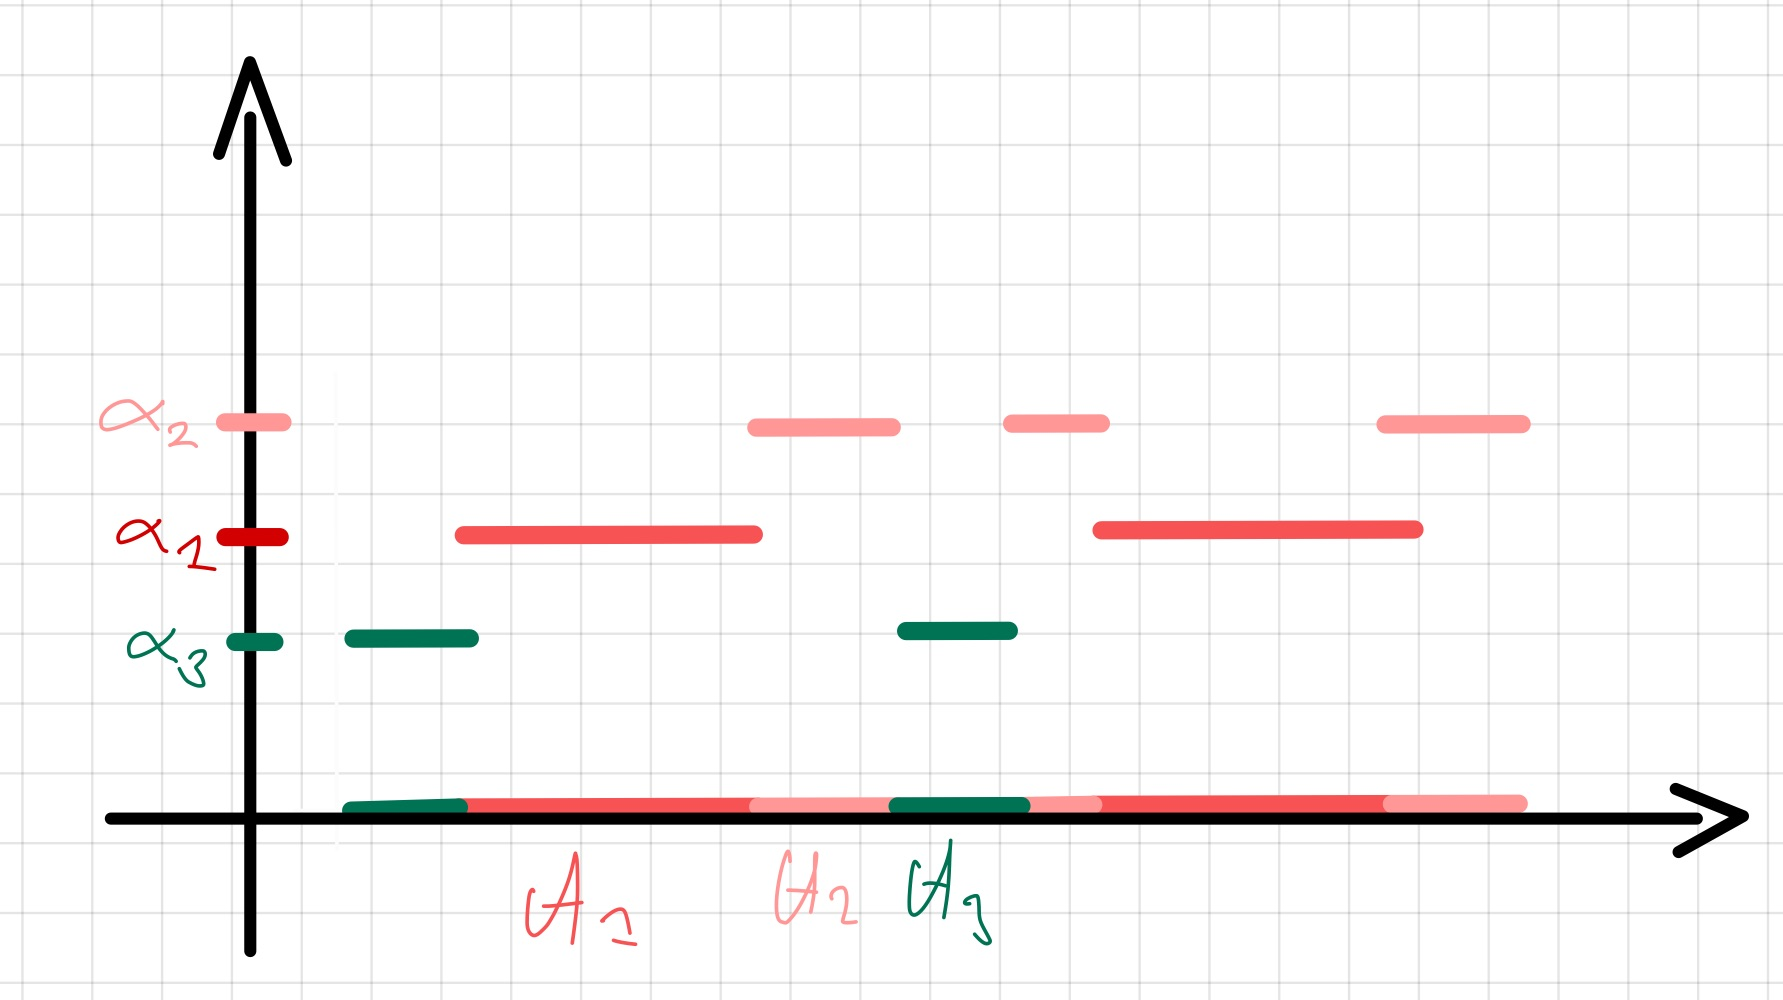
\includegraphics[width=\textwidth]{../\string_build/html/\string_images/simplefun.jpg}
\caption{Visualisierung einer einfachen Funktion.}\label{\detokenize{masstheorie/lebesgue_integral:fig-simplefun}}\end{figure}
\begin{definition}{}{masstheorie/lebesgue_integral:definition-7}



\par
Eine Funktion \(f:\R^n\to\overline{R}\) heißt einfach, falls Koeffizienten \(\alpha_i\in\overline{\R}\) und messbare Mengen \(A_i\in\mathcal{A}(\R^n)\) für \(i=1,\ldots,N\) existieren, s.d.,
\begin{align*}
f = \sum_{i=1}^N \alpha_i \bone_{A_i}.
\end{align*}\end{definition}

\par
Man erhält über die Definition direkt ein Lemma, dass einfache Funktionen Lebesgue messbar sind.
\begin{lemma}{}{masstheorie/lebesgue_integral:lemma-8}



\par
Es sei \(f:\R^n\to\overline{\R}\) eine einfache Funktion, dann ist \(f\) Lebesgue messbar.
\end{lemma}

\begin{proof}
 Siehe \href{https://www.fau.tv/clip/id/40589}{Vorlesung} ab Minute 8:45.
\end{proof}

\par
Für einfache Funktionen können wir analog zum Riemann Integral das Lebesgue Integral definieren, indem wir das Maß der einzelnen Mengen multipliziert mit den Funktionswerten summieren, welche eine einfache Funktion erzeugen.
\begin{remark}{(Wohldefiniertheit)}{masstheorie/lebesgue_integral:remark-9}



\par
Es ist wichtig anzumerken, dass für eine einfache Funktion \(f\) verschiedene Zerlegungen in Mengen \(A_i\) und Koeffizienten \(\alpha_i\) existieren. Allerdings erkennen wir, dass der Wert des Integrals unabhängig von der Wahl der Zerlegung ist und das Intergal somit wohldefiniert ist.
\end{remark}


\subsection{Das Lebesgue Integral nicht negativer Funktionen}
\label{\detokenize{masstheorie/lebesgue_integral:das-lebesgue-integral-nicht-negativer-funktionen}}
\par
Die wichtige Eigenschaft, welche die Betrachtung von einfachen Funktion so relevant macht, ist dass sich messbare Funktionen beliebig gut durch einfache Funktionen approximieren lassen. Diese Tatsache formulieren wir in folgendem Lemma.
\begin{lemma}{}{masstheorie/lebesgue_integral:lem:simplefun}



\par
Sei \(f \colon \Omega \to [0,\infty]\) eine Lebesgue messbare Funktion, dann existiert eine monoton wachsende Folge \((f_i)_{i_\in N}\) von einfachen Funktionen mit
\begin{align*}
f_i&\leq f_{i+1}\\
f_i &= 0\text{ in }\Omega^C\\
f&=\lim_{i\to\infty} f_i.
\end{align*}\end{lemma}

\begin{proof}
 Siehe \href{https://www.fau.tv/clip/id/40589}{Vorlesung} ab Minute 13:00.
\end{proof}

\par
Mithilfe der Tatsache, dass sich messbare Funktionen beliebig gut durch einfache Funktionen approximieren lassen, können wir nun das Lebesgue Integral für nicht negative messbare Funktionen einführen.
\begin{definition}{}{masstheorie/lebesgue_integral:definition-11}



\par
Es sei \(f:\Omega\to[0,\infty]\) Lebesgue messbar und nach \cref{masstheorie/lebesgue_integral:lem:simplefun} \((f_i)_{i\in\N}\) eine monoton wachsende Folge von einfachen Funktionen mit \(\lim_{i\to\infty} f_i = f\), dann ist das \textbf{Lebesgue Integral} von \(f\) definiert durch
\begin{align*}
\int_{\Omega} f \,d\lambda^n = \lim_{i\rightarrow \infty} \int_{\R^n} f_i \,d\lambda^n.
\end{align*}\end{definition}

\par
Wir zeigen im Folgenden wichtige Eigenschaften des Lebesgue Integrals.
\begin{theorem}{(Eigenschaften des Lebesgue Integrals)}{masstheorie/lebesgue_integral:theorem-12}



\par
Das Lebesgue Integral ist \emph{wohldefiniert}, d.h., sein Wert ist unabhängig von der gewählten Folge von einfachen Funktionen \((f_n)_{n\in\N}\).
Darüber hinaus ist das Lebesgue Integral \emph{linear} und \emph{monoton}, d.h., für nicht negative, Lebesgue messbare Funktionen \(f,g \geq 0,\alpha\in\overline{\R}\) gilt
\begin{align*}
\int_\Omega f+\alpha\,g\,d\lambda^n = \int_\Omega f\,d\lambda^n + \alpha\, \int_\Omega g d\lambda^n\\
f \leq g \quad \Rightarrow \quad \int_\Omega f\, d\lambda^n \leq \int_\Omega g\, d\lambda^n.
\end{align*}\end{theorem}

\begin{proof}
 Siehe \href{https://www.fau.tv/clip/id/40589}{Vorlesung} ab Minute 30:00.
\end{proof}

\par
Anstatt der Folge von einfachen Funktionen, kann man auch eine beliebige monotone Folge von messbaren Funktionen benutzen um das Integral zu approximieren. Diese Aussage ist unter dem \textbf{Satz von der monotonen Konvergenz} oder dem \textbf{Konvergenzsatz von Beppo Levi} bekannt.

\begin{emphBox}{Beppo Levi}{}

\par
\href{https://de.wikipedia.org/wiki/Beppo\_Levi}{Beppo Levi} (Geboren 14. Mai 1875 in Turin, Italien; Gestorben 28. August 1961 in Rosario, Argentinien) war ein italienischer Mathematiker.
\end{emphBox}
\begin{lemma}{}{masstheorie/lebesgue_integral:lem:levi}



\par
Es sei \(f_i:\R^n\to[0,\infty],i\in\N\) eine Folge nicht negativer Lebesgue messbarer Funktionen mit
\begin{align*}
f_i\leq f_{i+1}\qquad\text{(Monotonie))},\\
\lim_{i\to\infty} f_i = f\qquad\text{(Konvergenz)},
\end{align*}
\par
wobei \(f:[0,\infty]\to\overline{\R}\) auch Lebesgue messbar ist, dann gilt
\begin{align*}
\lim_{i\to\infty} \int_{\R^n} f_i \,d\lambda^n = \int_{\R^n} f \,d\lambda^n
\end{align*}\end{lemma}

\begin{proof}
 Ref missing.
\end{proof}

\par
Eine weitere Aussage in diesem Kontext ist das \textbf{Lemma von Fatou}, welches eine Abschätzung für eine nicht notwendigerweise konvergierende Folge von Funktionen zeigt.

\begin{emphBox}{Pierre Fatou}{}

\par
\href{https://de.wikipedia.org/wiki/Pierre\_Fatou}{Pierre Joseph Louis Fatou} (Geboren 28. Februar 1878 in Lorient; Gestorben 10. August 1929 in Pornichet) war ein französischer Mathematiker.
\end{emphBox}
\begin{lemma}{}{masstheorie/lebesgue_integral:lemma-14}



\par
Es sei \(f_i:\R^n\to[0,\infty],i\in\N\) eine Folge nicht negativer Lebesgue messbarer Funktion, dann ist
\begin{align*}
f(x) := \liminf_{i\to\infty} f_i(x)
\end{align*}
\par
nicht negativ und Lebesgue messbar und es gilt
\begin{align*}
\liminf_{i\to\infty} \int_{\R} f_i\, d\lambda^n \geq \int_\R^n f\, d\lambda^n.
\end{align*}\end{lemma}

\begin{proof}
 Ref missing.
\end{proof}


\subsection{Das Lebesgue Integral integrierbarer Funktionen}
\label{\detokenize{masstheorie/lebesgue_integral:das-lebesgue-integral-integrierbarer-funktionen}}
\par
Wir wollen nun das Lebesgue Integral auf messbaren Funktionen mit wechselndem Vorzeichen betrachten. Dafür spalten wir eine Funktionen in ihren positiven und ihren negativen Teil auf und bilden das Integral über diese Funktionen. Um die beiden Teile aufsummieren zu können, müssen wir allerdings fordern, dass beide endlich sind.
\begin{definition}{}{masstheorie/lebesgue_integral:definition-15}



\par
Sei \(f \colon \R^n \rightarrow \R\) eine Lebesgue messbare Funktion, wir nennen die Funktion \(f\) \textbf{Lebesgue integrierbar}, falls
\begin{align*}
\int_{\R^n} \abs{f} d\lambda^n < +\infty
\end{align*}
\par
gilt. Für eine Lebesgue integrierbare Funktion \(f\), definieren wir entsprechende positive integrierbare Funktionen
\begin{align*}
f^+ := \max \lbrace f, 0 \rbrace, \qquad f_- := \max{-f, 0},
\end{align*}
\par
so dass gilt \(f = f^+ - f_-\). Dann können wir das \textbf{Lebesgue Integral} von \(f\) definieren als
\begin{align*}
\int_{\R^n} f\, d\lambda^n := \int_{\R^n} f^+\, d\lambda^n - \int_{\R^n} f_-\, d\lambda^n.
\end{align*}\end{definition}
\begin{lemma}{}{masstheorie/lebesgue_integral:lemma-16}



\par
Das Lebesgue Integral ist ein linearer und monotoner Operator auf der Menge der Lebesgue integrierbaren Funktionen.
\end{lemma}

\begin{proof}
 ToDo
\end{proof}

\par
Auch für integrierbare Funktionen gibt es einen wichtigen Konvergenzsatz, der \textbf{Konvergenzsatz von Lebesgue} oder auch der \textbf{Satz von der dominierten Konvergenz}.
\begin{theorem}{}{masstheorie/lebesgue_integral:theorem-17}



\par
Es sei \(f_i:\R^n\to\R\) eine Folge Lebesgue messbarer Funktionen mit \(\lim_{i\to\infty} f_i =f\) und \(\abs{f}\leq g\) wobei \(g\) eine Lebesgue integrierbare Funktion ist, dann gilt \(f\) ist Lebesgue integrierbar und
\begin{align*}
\lim_{i\to\infty} \int_{\R^n} f_i\, d\lambda^n = \int_{\R^n} f\, d\lambda^n.
\end{align*}\end{theorem}

\begin{proof}
 Ref missing.
\end{proof}


\subsection{Fast überall Eigenschaften}
\begin{definition}{}{\detokenize{masstheorie/lebesgue_integral:fast-uberall-eigenschaften}}\label{masstheorie/lebesgue_integral:definition-18}



\par
Seien \(f,g \colon \R^n \rightarrow \overline{\R}\) Lebesgue messbare Funktionen.
Wir sagen \(f = g\) \textbf{fast sicher} bezüglich des Lebesgue Maßes genau dann, wenn eine Lebesgue Nullmenge \(N\) existiert, so dass gilt
\begin{align*}
f(x) = g(x) \quad \forall x \in \R^n \setminus N.
\end{align*}\end{definition}


\section{Integrationstechniken}
\label{\detokenize{masstheorie/integrationstechnik:integrationstechniken}}\label{\detokenize{masstheorie/integrationstechnik::doc}}
\par
In diesem Abschnitt beschäftigen wir uns mit Rechenmethoden und Rechenregeln, die es uns erlauben Funktionen mehrerer Variablen bezüglich des Lebesgue Maßes zu integrieren. Insbesondere lernen wir dadurch Verfahren kennen um Volumina und Flächen zu berechnen. Um diese Regeln formal zu zeigen benötigen wir zunächst etwas Theorie.


\subsection{Produktalgebren}
\label{\detokenize{masstheorie/integrationstechnik:produktalgebren}}
\par
Für zwei Messräume \((\Omega_1,\Sigma_1), (\Omega_2,\Sigma_2)\) wollen wir nun einen Produktraum erhalten. Hierbei werden wir auf Konzepte des \textbf{Tensorproduktes} zurückgreifen und benutzen deshalb die gleiche Notation. Wir definieren dann die Produkt \(\sigma\) Algebra,
\begin{align*}
\Sigma_1\otimes\Sigma_2 := \sigma\left(\Sigma_1\times\Sigma_2\right),
\end{align*}
\par
wobei
\begin{align*}
\Sigma_1\times\Sigma_2 = \left\{A_1\times A_2: A_1\in\Sigma_1, A_2\in\Sigma_2\right\}.
\end{align*}
\par
Wir arbeiten nicht auf Vektorräumen darum konstruieren wir \textbf{kein} Tensorprodukt im Sinnen von \hyperref[\detokenize{vektoranalysis/tensor:s-tensoren}]{Abschnitt \ref{\detokenize{vektoranalysis/tensor:s-tensoren}}}, aber die grundlegenden Konzepte sind ähnlich, weshalb es üblich ist, hier diese Notation zu verwenden. Weiterhin erkennen wir, dass mit dieser Konstruktion \(\Sigma_1\otimes\Sigma_2 \) eine \(\sigma\) Algebra auf \(\Omega_1\times\Omega_2\) ist.

\begin{figure}[htbp]
\centering


\noindent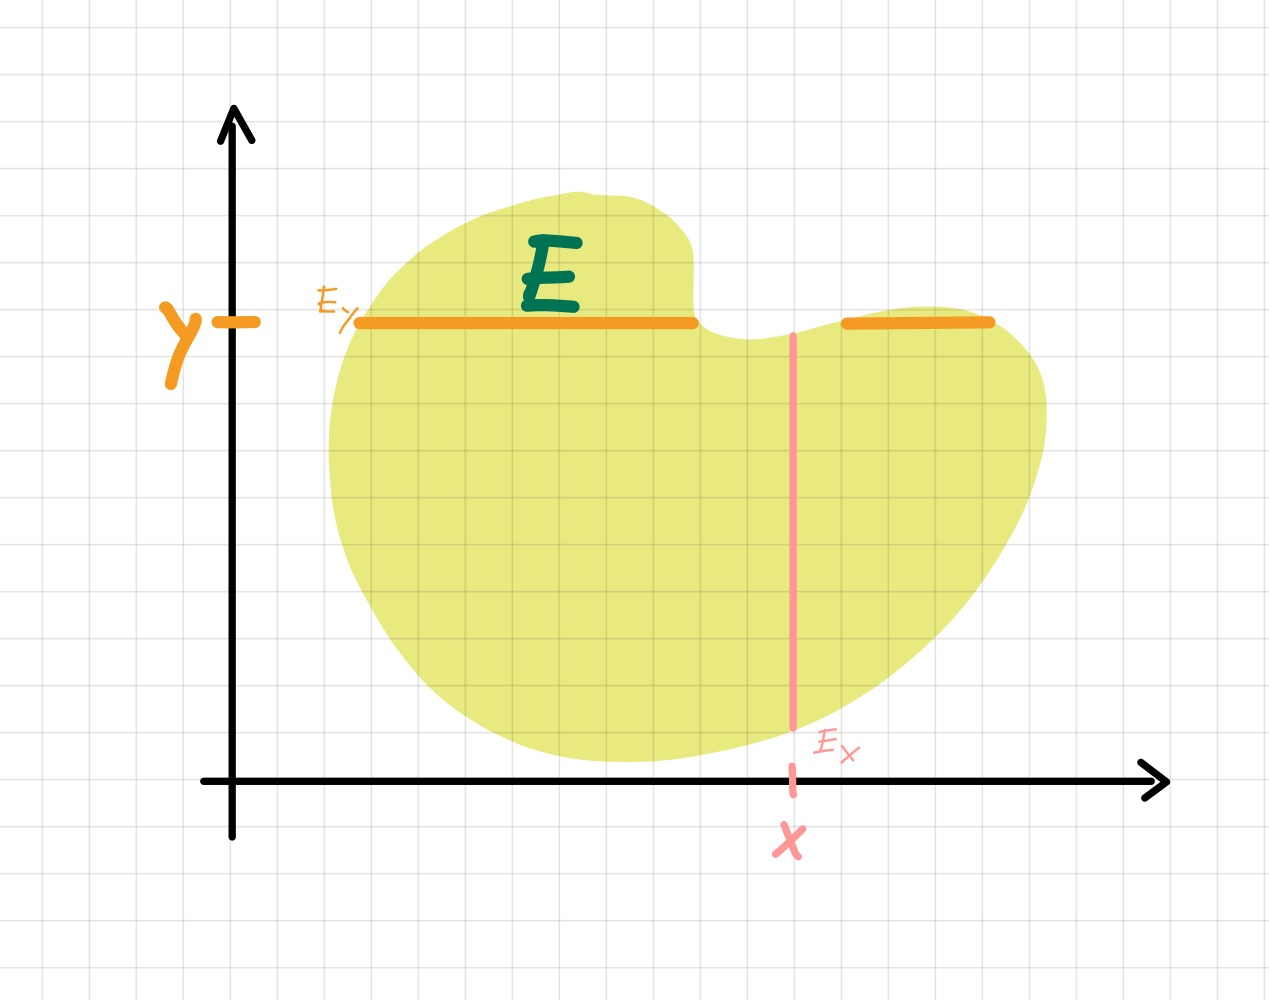
\includegraphics[width=\textwidth]{../\string_build/html/\string_images/schnitte.jpg}
\caption{Visualisierung von Mengenschnitten.}\label{\detokenize{masstheorie/integrationstechnik:fig-schnitte}}\end{figure}

\par
Für eine Menge \(E\subset\Omega_1\times\Omega_2\) betrachtet man in diesem Kontext oft sogenannte \textbf{Schnitte}
\begin{align*}
E_x := \{y\in \Omega_2: (x,y)\in E\}\subset\Omega_2\\
E^y := \{x\in \Omega_1: (x,y)\in E\}\subset\Omega_1
\end{align*}
\par
wofür man folgende Aussage hat.
\begin{lemma}{}{masstheorie/integrationstechnik:lem:secmeasure}



\par
Es seien \((\Omega_1,\Sigma_1), (\Omega_2,\Sigma_2)\) Messräume, dann gilt für eine Produktmessbare Menge \(E\in \Sigma_1\otimes\Sigma_2\), dass \(E_x\in \Sigma_2, E_y\in\Sigma_1\) für alle \(x\in\Omega_1,y\in\Omega_2\).
\end{lemma}

\begin{proof}
 Wir betrachten das Teilmengensystem
\begin{align*}
\M = \{E\subset\Omega_1\times\Omega_2:  E_x\in\Sigma_2, E^y\in\Sigma_1,\quad\forall x\in\Omega_1,  y\in\Omega_2\}
\end{align*}
\par
d.h. alle Mengen, welche die gewünschte Bedingung erfüllen. Wir sehen, dass für \(A\in\Sigma1,B\in\Sigma_2\) gilt
\begin{align*}
(A\times B)_x = 
\begin{cases}
B &\text{ falls }x\in A\\
\emptyset &\text{ sonst}
\end{cases}
\end{align*}
\par
und daher \((A\times B)_x\in\Sigma_2\) für alle \(x\in\Omega_1\). Analog zeigt man \((A\times B)^y\in\Sigma_1\) für alle \(y\in\Omega_2\) und daher gilt
\begin{align*}
\Sigma_1\times\Sigma_2\subset \M.
\end{align*}
\par
Weiterhin ist \(\M\) eine \(\sigma\) Algebra. Es gilt \(\emptyset\M\), weiterhin \((E^C)_x = (E_x)^C\)und analog \((E^C)^y= (E^y)^C\) und daher
gilt
\begin{align*}
E\in\M\Rightarrow E^C\in\M.
\end{align*}
\par
Weiterhin gilt für eine Folge von Mengen \(E_i\in\M,i\in\N\)
\begin{align*}
\left(\bigcup_{i\in\N} E_i\right)_x = \bigcup_{i\in\N} (E_i)_x
\end{align*}
\par
analog für den anderen Schnitt und daher
\begin{align*}
\bigcup_{i\in\N} E_i\in\M.
\end{align*}
\par
Somit folgt
\begin{align*}
\Sigma_1\otimes\Sigma_2=\sigma(\Sigma_1\times\Sigma_2)\subset \sigma(\M) = \M.
\end{align*}\end{proof}

\par
Speziell für \(\Omega_1=\R^n, \Omega_1=\R^m\) könnte man sich nun fragen wie sich die Produkt Algebra für die bekannten Borel und Lebesgue Algebren verhält. Zumindest für die Borel \(\sigma\) Algebra haben wir folgende Aussage.
\begin{lemma}{}{masstheorie/integrationstechnik:lemma-1}



\par
Für \(n,m\in\N\) gilt
\begin{align*}
\B(\R^n)\otimes \B(\R^m) = \B(\R^{n+m}).
\end{align*}\end{lemma}

\begin{proof}
 Offensichtlich gilt für den Mengen Ring
\begin{align*}
\mathcal{R}(\R^{n+m})=\left\{\bigcup_{i=1}^N Q_i: Q_i\subset\R^{n+m}\text{ ist halboffener Quader} \right\},
\end{align*}
\par
dass
\begin{align*}
\mathcal{R}(\R^{n+m})\subset \B(\R^n)\otimes \B(\R^m).
\end{align*}
\par
Weiterhin wissen wir aber auch nach \cref{masstheorie/masstheorie:s-gentop} , dass \(\sigma(\mathcal{R}(\R^{n+m})) = \B(\R^{n+m})\) und somit
\begin{align*}
\B(\R^{n+m})\subset \B(\R^n)\otimes \B(\R^m).
\end{align*}
\par
Für die andere Richtung sei \(A_1\in\B(\R^n) A_2\in\B(\R^m)\), dann gilt
\begin{align*}
A_1\times A_2 = \left(A_1\times\R^m\right) \cap (\R^n\times A_2) =\pi_1^{-1}(A_1) \cap \pi_2^{-1}(A_2)
\end{align*}
\par
wobei \(\pi_1:\R^{n+m}\to\R^n,\pi_2:\R^{n+m}\to\R^m\) die Projektionen
\begin{align*}
\pi_1(z_1,\ldots,z_{n+m})&= (z_1,\ldots, z_n)\\
\pi_2(z_1,\ldots,z_{n+m})&= (z_{n+1},\ldots, z_{n+m})
\end{align*}
\par
sind. Da Projektionen stetig sind, sind sie Borel messbar nach ?? und daher gilt
\begin{align*}
\pi_1^{-1}(A_1)\in B(\R^{n+m})\\
\pi_2^{-1}(A_2)\in B(\R^{n+m}).
\end{align*}
\par
Daraus folgern wir, dass
\begin{align*}
A_1\times A_2 \in \B(\R^{n+m})
\end{align*}
\par
und somit
\begin{align*}
\B(\R^n)\otimes \B(\R^m)\subset\B(\R^{n+m}).
\end{align*}\end{proof}

\par
Für die Lebesgue \(\sigma\) Algebren gilt diese Identität nicht, allgemein kann man zeigen, dass
\begin{align*}
\mathcal{A}(\R^n)\otimes\mathcal{A}(\R^m)\subset \mathcal{A}(\R^{n+m})
\end{align*}
\par
allerdings ist die Menge auf der rechten Seite echt größer wie das folgende Beispiel zeigt.
\begin{example}{}{masstheorie/integrationstechnik:ex:prodsig}



\par
Wir betrachten die zwei Lebesgue Algebren für \(n=m=1\), dh. \(\mathcal{A}(\R)\). Nach \hyperref[\detokenize{masstheorie/masstheorie:s-vitali}]{Abschnitt \ref{\detokenize{masstheorie/masstheorie:s-vitali}}} gibt es Mengen \(V\subset\R\) sogenannte Vitali Mengen s.d. \(V\not\in\mathcal{A}(\R)\). Weiterhin erkennen wir, dass für das Lebesgue Maß auf \(\R^2\) folgt, dass
\begin{align*}
\lambda^{2}(V\times\{0\}) = 0
\end{align*}
\par
dies folgt mit der Argumentation aus Aufgabe??. Daher ist \(V\times\{0\}\in \mathcal{A}(\R^2)\) da es eine Nullmenge ist.

\par
Wir erkennen aber, dass sich \(V\) als Schnitt dieser Produkt Menge darstellen lässt, nämlich
\begin{align*}
V = (V\times\{0\})^0
\end{align*}
\par
wäre nun \((V\times\{0\})^0\in \mathcal{A}(\R)\otimes\mathcal{A}(\R)\) so würde mit \cref{masstheorie/integrationstechnik:lem:secmeasure} folgen, dass auch der Schnitt \(V\in\mathcal{A}(\R)\) gilt, was ein Widerspruch ist, daher
\begin{align*}
(V\times\{0\})^0 \not\in  \mathcal{A}(\R)\otimes\mathcal{A}(\R).
\end{align*}\end{example}

\par
Das abstrakte Konzept, welches sich hinter diesem Beispiel verbirgt wir mit dem Begriff Vollständigkeit eines Maßes bezeichnet.
\begin{definition}{}{masstheorie/integrationstechnik:definition-3}



\par
Ein Maßraum \((\Omega,\Sigma,\mu)\), falls für jede \(\mu\) Nullmenge \(N\in\Sigma, \mu(N)=0\) gilt
\begin{align*}
A\subset N \Rightarrow A\in \Sigma.
\end{align*}\end{definition}
\begin{remark}{}{masstheorie/integrationstechnik:remark-4}



\par
Wir wissen, dass jede Menge die bezüglich des äußeren Maßes \(\lambda^\ast\) eine Nullmenge ist auch Lebesgue messbar ist. Daher ist das Lebesgue Maß ein vollständiges Maß.
\end{remark}

\par
Weiterhin lässt sich ein beliebiges Maß vervollständigen, indem wir die \(\sigma\) Algebra
\begin{align*}
\overline{\Sigma}:=\{A\cup N: A\in\Sigma, N\subset B\in\Sigma\text{ mit }\mu(B)=0\}
\end{align*}
\par
betrachten zusammen mit dem Maß
\begin{align*}
\overline{\mu}(B)= \overline{\mu}(A\cup N):= \mu(A).
\end{align*}
\par
Hier lässt sich nun folgendes zeigen.
\begin{lemma}{}{masstheorie/integrationstechnik:lem:completelebesgue}



\par
Für \(n,m\in\N\) gilt
\begin{align*}
\overline{\mathcal{A}(\R^n)\otimes\mathcal{A}(\R^m)}= \mathcal{A}(\R^{n+m}).
\end{align*}\end{lemma}

\begin{proof}
 Siehe z.B. \cite{Bog07} Theorem 1.5.6.
\end{proof}


\subsection{Produktmaße}
\label{\detokenize{masstheorie/integrationstechnik:produktmasze}}
\par
Wir wollen nun Maße auf der Produktalgebra betrachten.
\begin{definition}{}{masstheorie/integrationstechnik:definition-6}



\par
Es seien \((\Omega_1,\Sigma_1,\mu_1), (\Omega_2,\Sigma_2,\mu_2)\) zwei Maßräume, dann heißt ein Maß \(\mu\) auf dem Messraum \((\Sigma_1\otimes\Sigma_2, \Omega_1\times\Omega_2)\) \textbf{Produktmaß}, falls
\begin{align*}
\mu(A_1\times A_2) = \mu_1(A_1)\cdot\mu_2(A_2)\quad\forall A_1\in\Sigma_1, A_2\in\Sigma_2.
\end{align*}\end{definition}
\begin{remark}{}{masstheorie/integrationstechnik:remark-7}



\par
In \cref{vektoranalysis/tensor:s-grass}  haben wir das Tensorprodukt zweier lineare Abbildungen \(T_1,T_2\) definiert über
\begin{align*}
(T_1\otimes T_2)(v_1,V_2) := T_1(v_1)\cdot T_2(v_2).
\end{align*}
\par
Es sei hier erwähnt, dass das Maß \textbf{keine} lineare Abbildung ist, insbesondere haben wir keinen Vektorraum gegeben. Die Produktstruktur ist trotzdem ähnlich, weshalb eine gewisse Analogie zwischen dem Tensorprodukt und dem Produktmaß herrscht.
\end{remark}
\begin{remark}{}{masstheorie/integrationstechnik:remark-8}



\par
In den obigen Produkten können einzelnen Terme jeweils unendlich werden, hierbei benutzt man die Konvention
\begin{align*}
0 * a = 0\quad\forall a\in\overline{\R}.
\end{align*}\end{remark}

\par
Man kann zeigen, dass ein Produktmaß stets existiert siehe ??. Allerdings ist es nicht notwendigerweise eindeutig bestimmt, hierfür benötigt man die sogennate \(\sigma\) Endlichkeit.
\begin{definition}{}{masstheorie/integrationstechnik:definition-9}



\par
Es sei \((\Omega,\Sigma,\mu)\) ein Maßraum, das Maß \(\mu\) heißt \(\sigma\)\textbf{ endlich}, falls eine Folge von Mengen \(A_i\in\Sigma,i\in\N\) existiert, s.d., \(\mu(A_i)<\infty\) und
\begin{align*}
\bigcup_{i\in\N} A_i = \Omega.
\end{align*}\end{definition}
\begin{remark}{}{masstheorie/integrationstechnik:remark-10}



\par
Das wichtigste Beispiel für uns ist das Lebesgue Maß auf \(\R^n\) welches bezüglich der Borelschen \(\sigma\) Algebra zwar nicht endlich aber \(\sigma\) endlich ist. Insbesondere ist es damit auch \(\sigma\) endlich bezüglich der Lebesgue \(\sigma\) Algebra \(\mathcal{A}\).
\end{remark}

\par
Für \(\sigma\) endliche Maße kann man zeigen, dass ein eindeutig bestimmtes Produktmaß existiert.
\begin{theorem}{}{masstheorie/integrationstechnik:theorem-11}



\par
Es seien \((\Omega_1,\Sigma_1,\mu_1), (\Omega_2,\Sigma_2,\mu_2)\) zwei \(\sigma\) endliche Maßräume, dann existiert eine eindeutig bestimmtes Produktmaß
\begin{align*}
\mu_1\otimes \mu_2:\Sigma_1\otimes\Sigma_2\to[0,\infty],
\end{align*}
\par
s.d. die Bedingung
\begin{align*}
(\mu_1\otimes\mu_2)(A\times B) = \mu_1(A)\cdot\mu_2(B)\quad\forall A\in\Sigma_1, B\in\Sigma_2,
\end{align*}
\par
erfüllt ist.
\end{theorem}

\begin{proof}
 See Bogachev ref missing.
\end{proof}

\par
Anhand von \cref{masstheorie/integrationstechnik:ex:prodsig} haben wir gesehen, dass die Lebesgue \(\sigma\) Algebra auf \(\R^{n+m}\) größer ist als die Produkt \(\sigma\) Algebra. Allerdings kann man zeigen, dass das Produktmaß zumindest auf der kleineren Produktalgebra übereinstimmt.
\begin{lemma}{}{masstheorie/integrationstechnik:lem:lebesguecomp}



\par
Es gilt
\begin{align*}
\lambda^{n+m} = \overline{\lambda^n\otimes\lambda^m},
\end{align*}
\par
insbesondere folgt damit für eine beliebige Menge \(E\in \mathcal{A}(\R^n)\otimes\mathcal{A}(\R^m)\)
\begin{align*}
\lambda^{n+m}(E) = (\lambda^n\otimes\lambda^m)(E).
\end{align*}\end{lemma}

\begin{proof}
 Siehe z.B. \cite{Bog07} Theorem 1.5.6.
\end{proof}

\par
Speziell für \(A_1\in\mathcal{A}(\R^n), A_2\in\mathcal{A}(\R^m)\) folgt damit
\begin{align*}
\lambda^{n+m}(A^1\times A^2)=\lambda^{n}(A^1)\cdot\lambda^{m}(A^2).
\end{align*}

\subsection{Das Prinzip von Cavalieri}
\label{\detokenize{masstheorie/integrationstechnik:das-prinzip-von-cavalieri}}
\par
Im vorherigen Abschnitt haben wir Produkte von Maßen betrachtet. Insbesondere haben wir erkannt, dass wir für Mengen der Form \(A\times B\), dass Lebesgue Maß multiplikativ aufteilen können,
\begin{align*}
\lambda^{n+m}(A\times B) = \lambda^n(A)\,\lambda^m(B).
\end{align*}
\par
Unser Ziel ist es nun das Lebesgue Maß beliebige messbare Mengen \(E\subset\R^{n+m}\) mithilfe der niedrigdimesnionaleren Lebesgue Maße auszudrücken. Dies führt auf das sogenannte Prinzip von Cavalieri.

\begin{emphBox}{Bonaventura Cavalieri}{}

\par
\href{https://de.wikipedia.org/wiki/Bonaventura\_Cavalieri}{Bonaventura Francesco Cavalieri} (Geboren 1598 wahrscheinlich in Mailand; Gestorben 3. Dezember oder 30. November 1647 in Bologna; mit Gelehrtennamen Cavalerius) war ein italienischer Jesuat, Mathematiker und Astronom.
\end{emphBox}

\begin{figure}[htbp]
\centering


\noindent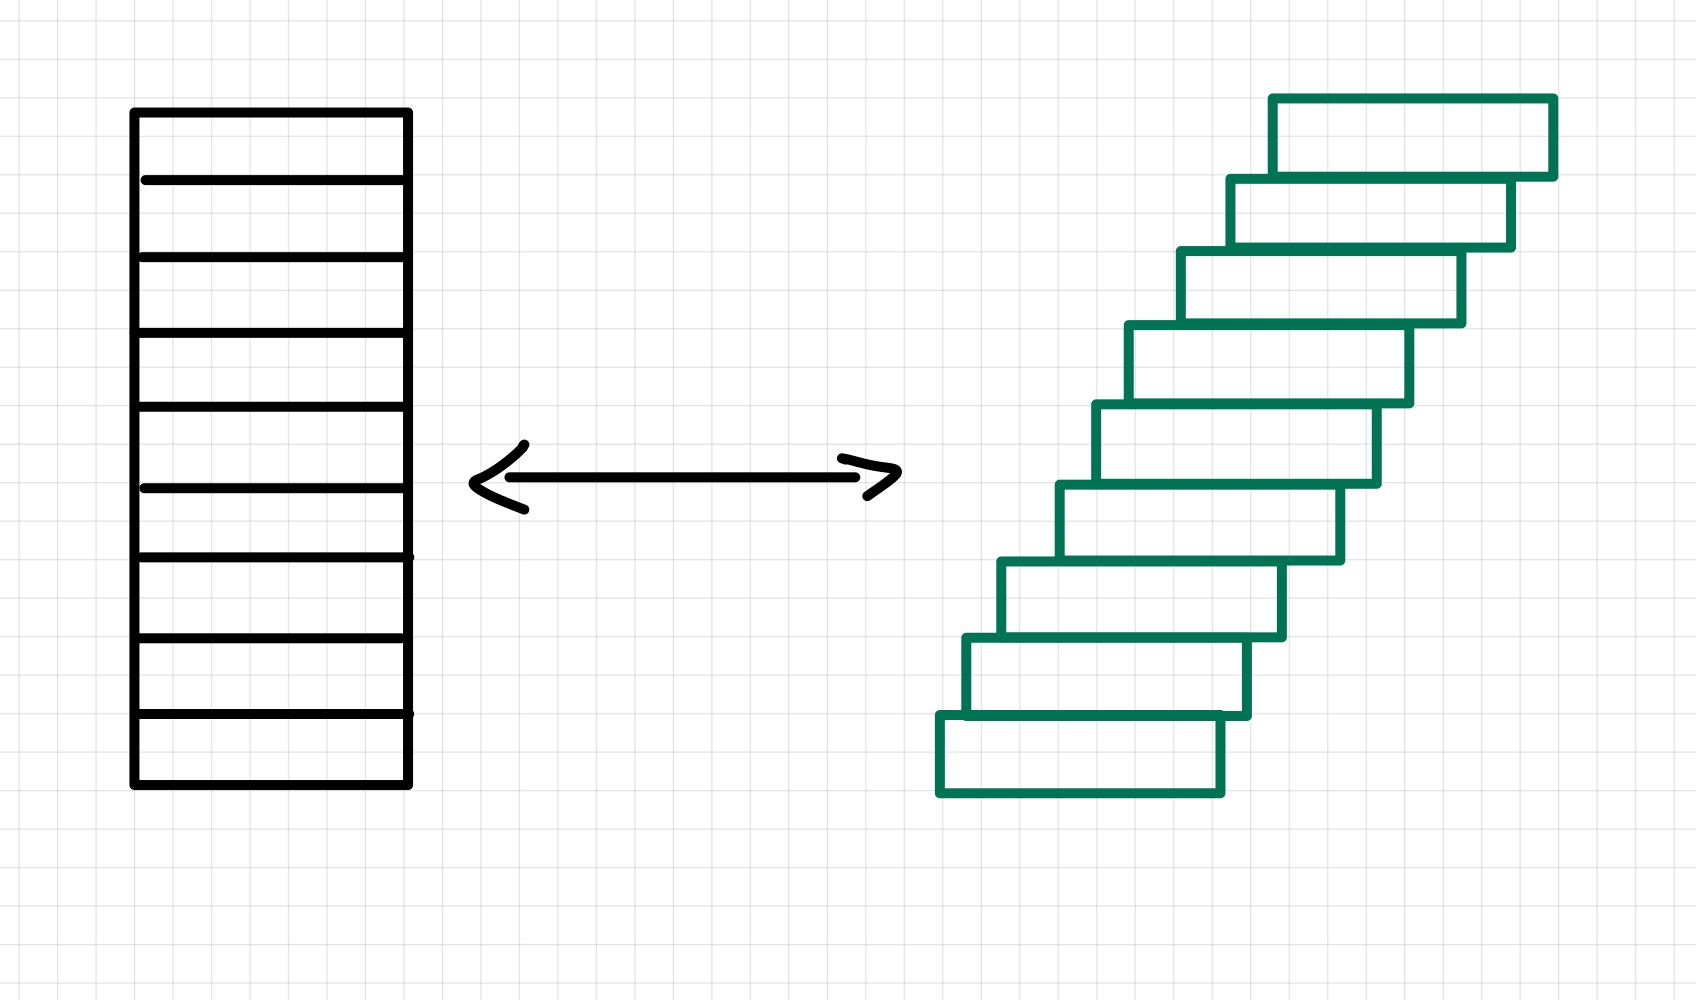
\includegraphics[width=\textwidth]{../\string_build/html/\string_images/cavalieri.jpg}
\caption{Visualisierung für das Prinzip von Cavalieri, beide Objekte haben die gleiche Fläche.}\label{\detokenize{masstheorie/integrationstechnik:fig-cavalieri}}\end{figure}

\par
Das Prinzip beruht auf der Intuition, dass zwei Körper, das gleiche Volumen haben, sofern alle ihre Schnittflächen welche parallel zu einer Grundfläche verlaufen gleich sind. Für \(\R^2\) ist dieses Prinzip in \hyperref[\detokenize{masstheorie/integrationstechnik:fig-cavalieri}]{Abb.\@ \ref{\detokenize{masstheorie/integrationstechnik:fig-cavalieri}}} dargestellt. Formal bedeutet das, dass wir für eine messbare Menge \(E\), den Inhalt über das Integral der Schnitte ausdrücken wollen, es gibt hier also drei Größen
\begin{align*}
\lambda^{n+m}(E), \int_{\R^n} \lambda^m(E_x) d\lambda^n(x), \int_{\R^m} \lambda^m(E_y) d\lambda^m(y)
\end{align*}
\par
welche wir in Beziehung zueinander setzten wollen.

\par
Ein Konzept was man in diesem Kontext benötigt, sind sogenannte monotone Klassen.
\begin{definition}{}{masstheorie/integrationstechnik:definition-13}



\par
Es sei \(\Omega\) eine Menge, ein Teilmengensystem \(\mathcal{C}\subset 2^\Omega\) heißt \textbf{monotone Klasse}, falls

\par
1. Für eine aufsteigende Folge von Mengen \(A_i\in\mathcal{C}, A_i\subset A_{i+1}, i\in\N\) gilt auch
\begin{align*}
\bigcup_{i\in\N} A_i\in\mathcal{C}.
\end{align*}
\par
1. Für eine absteigende Folge von Mengen \(A_i\in\mathcal{C}, A_i\supset A_{i+1}, i\in\N\) gilt auch
\begin{align*}
\bigcap_{i\in\N} A_i\in\mathcal{C}.
\end{align*}\end{definition}

\par
Offensichtlich ist jede \(\sigma\) Algebra eine monotone Klasse,die Umkehrung dieser Aussage gilt nicht im Allgemeinen.
Weiterhin arbeiten wir in diesem Kontext zusätzlich mit Mengenalgebren anstatt nur mit Mengenringen.
\begin{definition}{}{masstheorie/integrationstechnik:definition-14}



\par
Es sei \(\mathcal{R}\) ein Mengenring über der Menge \(\Omega\), gilt auch \(\Omega\in\mathcal{R}\), dann nennen wir \(\mathcal{R}\) \textbf{Mengenalgebra}.
\end{definition}
\begin{remark}{}{masstheorie/integrationstechnik:remark-15}



\par
Für zwei \(\sigma\) Algebren ist das kartesische Produkt \(\Sigma_1\times\Sigma_2\) i.A. keine Mengenalgebra, die Menge
\begin{align*}
\Sigma_1\diamond\Sigma_2:= \left\{\bigcup_{i=1}^N A^1_i\times A^2_i: A^1_i\in\Sigma_1, A^2_i\in\Sigma_2\quad i=1,\ldots,n\right\}
\end{align*}
\par
allerdings schon und sie erzeugt offensichtlich auch die Produkt \(\sigma\) Algebra,
\begin{align*}
\sigma(\Sigma_1\diamond\Sigma_2) = \Sigma_1\otimes\Sigma_2.
\end{align*}\end{remark}

\par
Betrachtet man analog zur kleinsten von \(\mathcal{C}\) erzeugten \(\sigma\) Algebra die kleinste von \(\mathcal{C}\) erzeugt monotone Klasse \(\text{M}\big[\mathcal{C}\big]\) so gilt folgendes hilfreiches Lemma.
\begin{lemma}{}{masstheorie/integrationstechnik:lem:monclass}



\par
Es sei \(\mathcal{C}\) eine Mengenalgebra, dann gilt
\begin{align*}
\sigma(\mathcal{C}) = \text{M}\big[\mathcal{C}\big].
\end{align*}\end{lemma}

\begin{proof}
 Siehe z.B. \cite{Tao07} Lemma 1.7.14.
\end{proof}

\par
Mithilfe des monotone Klassen Lemmas und den vorherigen Überlegungen können wir nun das Prinzip von Cavalieri beweisen.
\begin{theorem}{}{masstheorie/integrationstechnik:thm:cavalieri}



\par
Sei \(E \in \mathcal{A}(\R^n)\otimes\mathcal{A}(\R^m)\) mit \(\lambda^{n}\otimes\lambda^{m}(E) < \infty\),
dann gilt für fast alle \(x\in\R^n,y\in\R^m\), dass die Schnitte \(E_x, E^y\) auch Lebesgue messbar sind, die Funktionen
\begin{align*}
x \mapsto \lambda^m(E_x)\\
y \mapsto \lambda^n(E^y)
\end{align*}
\par
sind messbar und es gilt
\begin{align*}
\lambda^{n}\otimes\lambda^{m}(E) &= \int_{\R^n} \lambda^m(E_x) d\lambda^n(x)\\
&=
\int_{\R^m} \lambda^n(E^y) d\lambda^m(y).
\end{align*}\end{theorem}

\begin{proof}
 Es sei \(\mathcal{C}\subset\mathcal{A}(\R^n)\otimes\mathcal{A}(\R^m)\) das System aller Mengen s.d. die Aussage gilt. Dann ist \(\mathcal{C}\) eine monotone Klasse und
\begin{align*}
\mathcal{A}(\R^n)\diamond\mathcal{A}(\R^m)\subset \mathcal{C}.
\end{align*}
\par
Mit dem monotone Klassen Lemma (\cref{masstheorie/integrationstechnik:lem:monclass}  folgt dann
\begin{align*}
\mathcal{A}(\R^n)\otimes\mathcal{A}(\R^m) = \sigma(\mathcal{A}(\R^n)\diamond\mathcal{A}(\R^m)) = 
\text{M}\big[\mathcal{A}(\R^n)\diamond\mathcal{A}(\R^m)\big] \subset 
\text{M}\big[\mathcal{C}\big] = \mathcal{C}.
\end{align*}\end{proof}

\par
Ein Korollar aus der obigen Aussage ist, dass fast alle Schnitte einer \(\lambda^n\otimes\lambda^m\) Nullmenge selbst Nullmengen bezüglich \(\lambda^n\), bzw. \(\lambda^m\) sind.
\label{masstheorie/integrationstechnik:cor:zeroprodset}
\begin{emphBox}{}{}{Corollary 5.2}



\par
Es sei \(E\in\mathcal{A}(\R^n)\otimes\mathcal{A}(\R^m)\) eine Nullmenge, dann folgt, dass für fast alle \(x\in\R^n,y\in\R^m\) auch \(\lambda^m(E_x)=0=\lambda^n(E^y)\) gilt.
\end{emphBox}

\begin{proof}
 Für die Funktion \(f:x\mapsto \lambda^m(E_x)\) gilt mit dem Prinzip von Cavalieri, dass
\begin{align*}
0 = \lambda^{n}\otimes\lambda^{m}(E) = \int_{\R^n} f(x)d\lambda^n(x)
\end{align*}
\par
und daher mit ??, dass
\begin{align*}
f(x)=\lambda^m(E_x)=0
\end{align*}
\par
für fast alle \(x\in\R^n\). Die Aussage für \(\lambda^n(E^y)\) folgt analog.
\end{proof}

\par
Diese Korollar erlaubt es uns die Aussage von Cavalieri auf alle Mengen \(E\in \mathcal{A}(\R^{n+m})\) zu verallgemeinern.
\begin{lemma}{}{masstheorie/integrationstechnik:lemma-19}



\par
Die Aussage von \cref{masstheorie/integrationstechnik:thm:cavalieri} gilt auch für Mengen \(E\in \mathcal{A}(\R^{n+m})\).
\end{lemma}

\begin{proof}
 Es sei \(E\in \mathcal{A}(\R^{n+m})\), nach \cref{masstheorie/integrationstechnik:lem:completelebesgue} existieren Mengen \(\tilde{E}\in\mathcal{A}(\R^n)\otimes\mathcal{A}(\R^m)\), \(N\subset \tilde{N}\), s.d.
\begin{align*}
E = \tilde{E}\cup N\\
(\lambda^n\otimes\lambda^m)(\tilde{N}) = 0.
\end{align*}
\par
Insbesondere ist dann
\begin{align*}
E\setminus \tilde{N} = \left(\tilde{E}\setminus \tilde{N} \right)\cup \underbrace{\left(N\setminus \tilde{N}\right)}_{=\emptyset} = 
\tilde{E}\setminus \tilde{N}\in \in\mathcal{A}(\R^n)\otimes\mathcal{A}(\R^m)
\end{align*}
\par
daher können wir \cref{masstheorie/integrationstechnik:thm:cavalieri} auf \(E\setminus \tilde{N}\) anwenden. Da aber fast alle Schnitte \(\tilde{N}_x,\tilde{N}^y\) Nullmengen sind, gilt die Aussage, dann für fast alle \(x,y\in E\).
\end{proof}

\par
Mit dieser Aussage können wir nun ein Beispiel betrachten, in welchem wir die Fläche eines Kreises berechnen.

\begin{figure}[htbp]
\centering


\noindent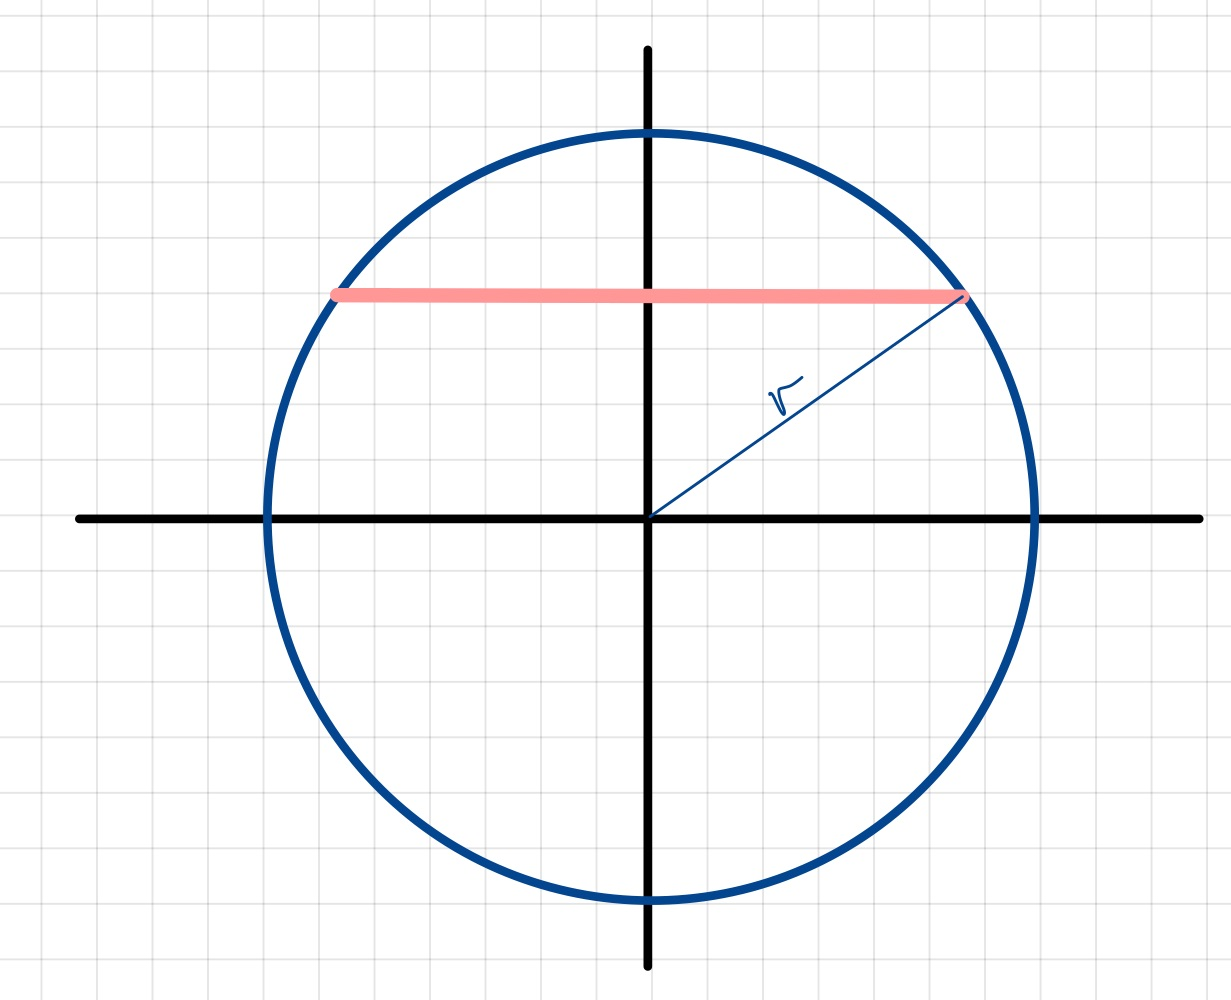
\includegraphics[width=\textwidth]{../\string_build/html/\string_images/ball.jpg}
\caption{Visualisierung für \cref{masstheorie/integrationstechnik:ex:ball} }\label{\detokenize{masstheorie/integrationstechnik:fig-ball}}\end{figure}
\begin{example}{}{masstheorie/integrationstechnik:ex:ball}



\par
Wir betrachten den \(2\) dimensionale Ball
\begin{align*}
B_r^2:=\{x\in\R^2: |x|\leq r\},
\end{align*}
\par
wir erkennen, dass sich ein Schnitt für \(\abs{y}\leq r\) jeweils ergibt durch
\begin{align*}
(B_r^2)_y = \{x:(x,y)\in B_r^2\} = \{x\leq\sqrt{r^2-y^2}\} = [-\sqrt{r^2-y^2},\sqrt{r^2-y^2}]
\end{align*}
\par
und ansonsten leer ist.

\par
Somit erhalten wir
\begin{align*}
\lambda^1((B_r^2)_y) = 
\begin{cases}
2 \sqrt{r^2-y^2}&\text{ falls }y\leq r\\
\emptyset\text{ sonst}
\end{cases}.
\end{align*}
\par
Damit erhalten wir mithilfe des Prinzips von Cavalieri
\begin{align*}
\lambda^2(B_r^2) &= \int_{\R} \lambda^1((B_r^2)_y) d\lambda^1(y) = 
\int_{[-r,r]} 2 \sqrt{r^2-y^2} d\lambda^1(y)\\
&= 
2\int_{-r}^r \sqrt{r^2 - y^2} dy = 
\lim_{t\to r}\left[y \sqrt{r^2-y^2} +r^2\arctan\left(\frac{y}{\sqrt{r^2-y^2}}\right)\right]^t_{-t}\\
&=
r^2\pi.
\end{align*}\end{example}

\par
Das Volumen einer Kugel in \(n\) Dimensionen lässt sich mithilfe des folgenden Lemmas berechnen.
\begin{lemma}{}{masstheorie/integrationstechnik:lemma-21}



\par
Für die \(n\) dimensionale Kugel
\begin{align*}
B_r^n:=\{x\in\R^n: |x|\leq r\}
\end{align*}
\par
gilt
\begin{align*}
\lambda^n(B_r^n) =
r^d\,
\begin{cases}
\frac{1}{(n/2)!} \pi^{n/2}&\text{ falls }n \text{ gerade,}\\
\frac{2}{1\cdot 3\cdot\ldots n} \pi^{(n-1)/2}&\text{ falls }n \text{ ungerade.}
\end{cases}
\end{align*}\end{lemma}

\begin{proof}
 Siehe Hausaufgabe.
\end{proof}


\subsection{Der Satz von Tonelli Fubini}
\label{\detokenize{masstheorie/integrationstechnik:der-satz-von-tonelli-fubini}}
\par
Das Prinzip von Cavalieri erlaubt es uns nun das Maß einer Menge über ihr das Produktmaß bzw. über Integrale auszudrücken. Insbesondere gilt für Indikatorfunktionen und messbare Mengen \(E\in\mathcal{A}(\R^{n+m})\), dass
\begin{align*}
\int_{\R^{n+m}} \bone_E d\lambda^{n+m} = \int_{\R^{n}} \int_{\R^{m}} \bone_{E_x}(y) d\lambda^m(y)d\lambda^n(x) =
\int_{\R^{m}} \int_{\R^{n}} \bone_{E_y}(x) d\lambda^m(x)d\lambda^n(y).
\end{align*}
\par
Da das Integral aber gerade über einfache Funktionen und somit über Indikatorfunktionen definiert ist, liegt die Vermutung nahe, dass die Aussage auch für beliebige messbare Funktionen \(f:\R^{n+m}\to\overline{R}\) gilt. Dieses Resultat ist als \emph{Satz von Tonelli} bekannt und erlaubt uns Integrale über Funktionen mehrere Variablen durch Doppelintegrale darzustellen. Hierbei ist jedoch anumerken, dass der Satz von Tonelli \textbf{nur} für nicht negative Funktionen gilt.

\begin{emphBox}{Leonida Tonelli}{}

\par
\href{https://de.wikipedia.org/wiki/Leonida\_Tonelli}{Leonida Tonelli} (Geboren 19. April 1885 in Gallipoli (Lecce); Gestorben 12. März 1946 in Pisa) war ein italienischer Mathematiker, ein Schüler von \href{https://de.wikipedia.org/wiki/Cesare\_Arzel\%C3\%A0}{Cesare Arzelà}.
\end{emphBox}
\begin{theorem}{}{masstheorie/integrationstechnik:thm:tonelli}



\par
Es sei \(f:\R^{n+m}\to [0,\infty]\) eine Lebesgue messbare Funktion, dann gilt für fast alle \(x\in\R^n,y\in\R^m\), dass die Funktionen \(x\mapsto f(x,y), y\mapsto f(x,y)\) auch Lebesgue messbar sind. Insbesondere sind auch die Funktionen
\begin{align*}
x \mapsto \int_{\R^m} f(x,y) d\lambda^m(y)\\
y \mapsto \int_{\R^n} f(x,y) d\lambda^n(x)
\end{align*}
\par
messbar und es gilt
\begin{align*}
\int_{\R^{n+m}} f(x,y) d\lambda^{n+m}(x,y) &= \int_{\R^n}\int_{\R^m} f(x,y) d\lambda^{n}(x)d\lambda^m(y)\\
&=
\int_{\R^m}\int_{\R^n} f(x,y) d\lambda^{m}(y)d\lambda^n(x).
\end{align*}\end{theorem}

\begin{proof}
 Man beweist die Aussage zunächst für Funktionen \(f:\R^{n+m}\to\overline{R}\) welche bezüglich \(\mathcal{A}(\R^n)\otimes\mathcal{A}(\R^m)\) messbar sind. Hierfür erkennt man durch mehrfache Anwendung des Satzes von Beppo Levi (\cref{masstheorie/lebesgue_integral:lem:levi}  unter Ausnutzung der \(\sigma\) Endlichkeit von \(\mathcal{A}(\R^n)\) und \(\mathcal{A}(\R^m)\), dass es reicht die Aussage auf Mengen endlichen Maßes zu zeigen. Da sich nach \cref{masstheorie/lebesgue_integral:lem:simplefun} aber jede Funktion durch einfache Funktionen approximieren lässt und das Integral linear ist, reicht es die Aussage für Indikatorfunktionen zu zeigen. Hier folgt die Aussage aber aus dem Prinzip von Cavalieri, \cref{masstheorie/integrationstechnik:thm:cavalieri} 

\par
Benutzten wir nun \cref{masstheorie/integrationstechnik:cor:zeroprodset} so folgt die Behauptung auch für Funktionen welche bezüglich \(\mathcal{A}(\R^{n+m})\) messbar sind.
\end{proof}

\par
In der obigen Aussage haben wir gefordert, dass die Funktionen nicht negativ sind. Um eine analogen Aussage auch für Funktionen mit wechselndem Vorzeichen zu erhalten müssen wir fordern, dass
\begin{align*}
\int_{\R^{n+m}} \abs{f(x,y)} d\lambda^{n+m}(x,y) <\infty
\end{align*}
\par
gilt. Dies ist Aussage des Satzes von Fubini.

\begin{emphBox}{Guido Fubini}{}

\par
\href{https://de.wikipedia.org/wiki/Guido\_Fubini}{Guido Fubini} (Geboren 19. Januar 1879 in Venedig; Gestorben 6. Juni 1943 in New York) war ein italienischer Mathematiker.
\end{emphBox}
\begin{theorem}{}{masstheorie/integrationstechnik:thm:fubini}



\par
Es sei \(f:\R^{n+m}\to \overline{\R}\) eine Lebesgue \textbf{integrierbare} Funktion, dann gilt für fast alle \(x\in\R^n,y\in\R^m\), dass die Funktionen \(x\mapsto f(x,y), y\mapsto f(x,y)\) auch Lebesgue messbar sind. Insbesondere sind auch die Funktionen
\begin{align*}
x \mapsto \int_{\R^m} f(x,y) d\lambda^m(y)\\
y \mapsto \int_{\R^n} f(x,y) d\lambda^n(x)
\end{align*}
\par
messbar und es gilt
\begin{align*}
\int_{\R^{n+m}} f(x,y) d\lambda^{n+m}(x,y) &= \int_{\R^n}\int_{\R^m} f(x,y) d\lambda^{n}(x)d\lambda^m(y)\\
&=
\int_{\R^m}\int_{\R^n} f(x,y) d\lambda^{m}(y)d\lambda^n(x).
\end{align*}\end{theorem}

\begin{proof}
 Folgt aus dem Satz von Tonelli, \cref{masstheorie/integrationstechnik:thm:tonelli} 
\end{proof}


\subsection{Die Jacobische Transformationsformel}
\label{\detokenize{masstheorie/integrationstechnik:die-jacobische-transformationsformel}}
\par
Die Intuition hinter dem Prinzip von Cavalieri ist, dass man über parallele Schnitte integriert und erkennt, dass das Volumen so erhalten bleibt. Wir fragen uns nun, wie sich das Volumen verhält, wenn man zwei Mengen vergleicht deren parallele Schnitte nicht unbedingt gleich sind, aber welche über eine Abbildung ineinander überführbar sind.

\begin{figure}[htbp]
\centering


\noindent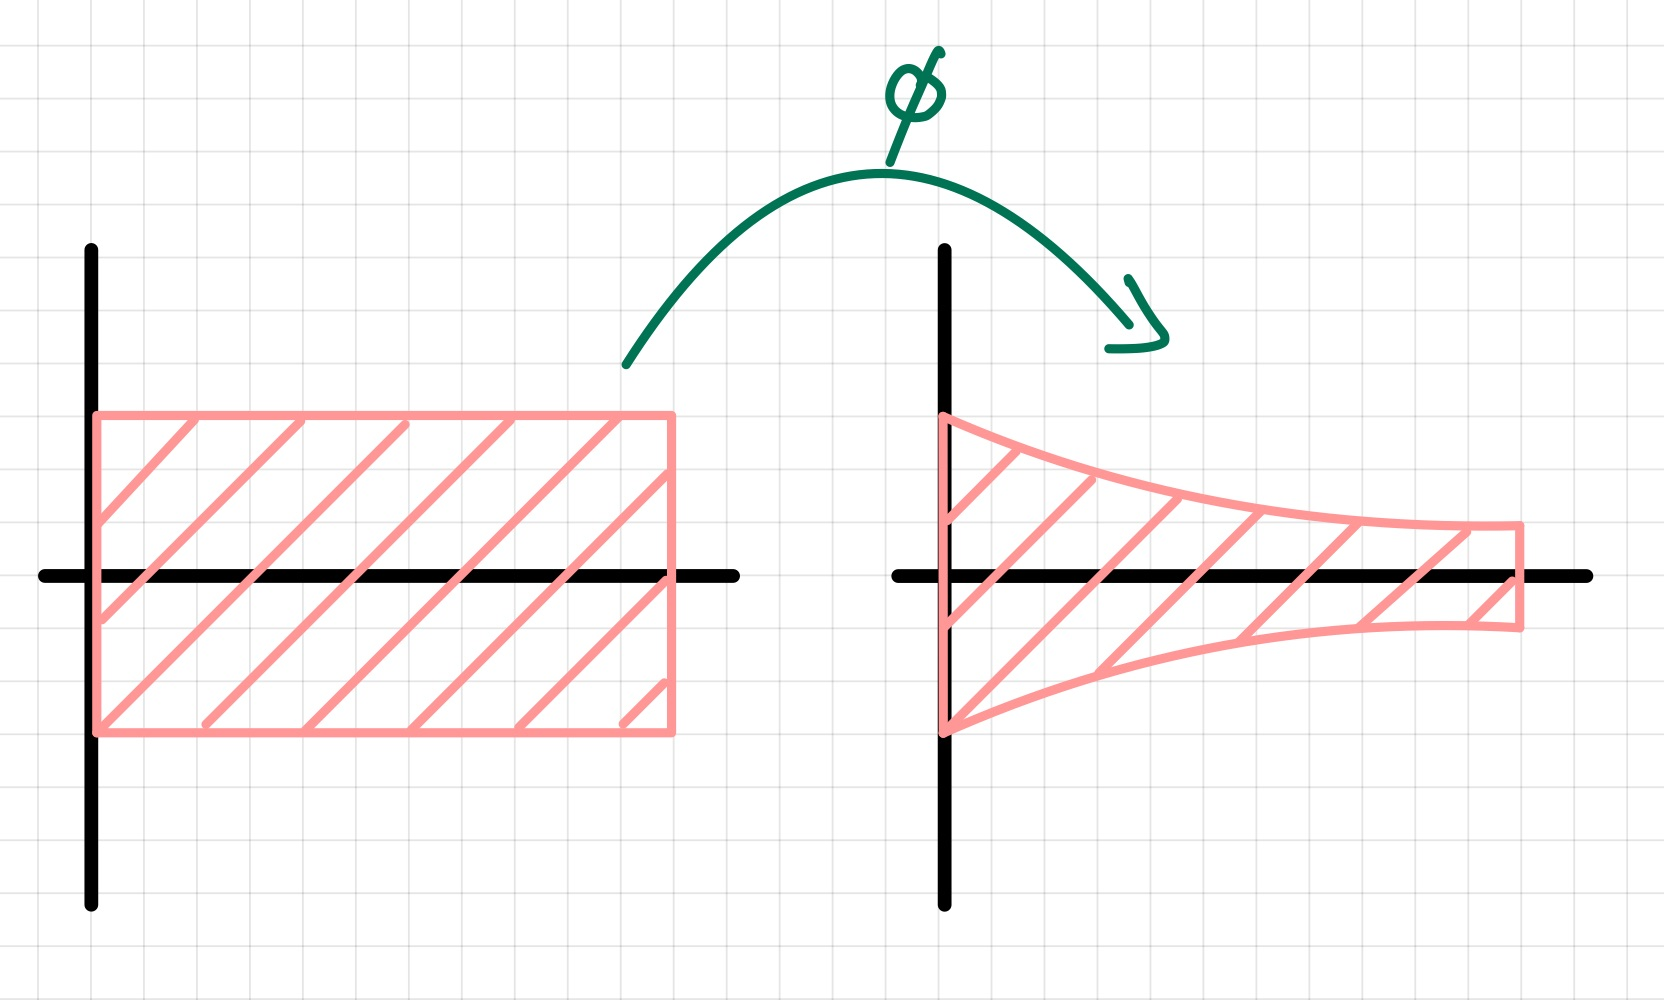
\includegraphics[width=\textwidth]{../\string_build/html/\string_images/trafo.jpg}
\caption{Visualisierung von Mengentransformationen.}\label{\detokenize{masstheorie/integrationstechnik:fig-trafo}}\end{figure}

\par
In \cref{masstheorie/masstheorie:rem:transinvariance} haben wir eine Matrix \(M\) und eine Menge \(M\) bereits die Identität
\begin{align*}
\lambda(MA) = |\det(M)| \, \lambda(A)
\end{align*}
\par
kennengelernt. Wir verllgemeinern diese Aussage nun, indem wir beliebige \(C^1\) Diffeomorphismen betrachten.
\begin{theorem}{}{masstheorie/integrationstechnik:thm:jacobitransformation}



\par
Seien \(U, V \subset \R^n\) offene Teilmengen und die Abbildung
\begin{align*}
\Phi \colon U \rightarrow V := \Phi(U)
\end{align*}
\par
sei ein \(C^1\) Diffeomorphismus, d.h., dass die Abbildung \(\Phi\) invertierbar ist, und dass sowohl \(\Phi\) als auch die Umkehrabbildung \(\Phi^{-1}\) stetig differenzierbar sind.
Sei außerdem \(f \colon V \rightarrow \R\) eine Lebesgue integrierbare Funktion.

\par
Dann gilt, dass die Verknüpfung \(f \circ \Phi \colon U \rightarrow \R\) auch Lebesgue integrierbar ist und es gilt die folgende Integrationsregel
\begin{align*}
\int_{\Phi(U)} f(y) \mu(\mathrm{d}y) = \int_U (f \circ \Phi)(x) \cdot |\det(D\Phi(x))|\mu(\mathrm{d}x).\end{align*}
\par
Hierbei nennt man \(\det(D\Phi(x))\) die \textbf{Jacobi Determinante}.
\end{theorem}

\begin{proof}
 Siehe z.B. \cite{Bog07} Theorem 3.7.1.
\end{proof}
\begin{remark}{}{masstheorie/integrationstechnik:remark-25}



\par
Für \(n=1\) ist diese Regel schon als Substitutionsregel bekannt.
\end{remark}
\begin{example}{}{masstheorie/integrationstechnik:example-26}



\par
ToDo
\end{example}


\chapter{Integration über Flächen und Mannigfaltigkeiten}
\label{\detokenize{surfaceintegrals/surfaceintegrals:integration-uber-flachen-und-mannigfaltigkeiten}}\label{\detokenize{surfaceintegrals/surfaceintegrals::doc}}

\chapter{Funktionentheorie}
\label{\detokenize{complexanalysis/complexanalysis:funktionentheorie}}\label{\detokenize{complexanalysis/complexanalysis::doc}}
\par
Im letzten Kapitel der Vorlesung widmen wir uns der \emph{Funktionentheorie}.
Diese befasst sich hauptsächlich mit der Theorie differenzierbarer komplexer Funktionen.
Da viele Konzepte der reellen Analysis verwendet werden, wird dieses Gebiet auch häufig \textbf{komplexe Analysis} genannt.

\par
Die Grundlagen des Körpers der komplexen Zahlen wurden bereits in {[}{]} behandelt.


\section{Cauchy Riemann Gleichungen}
\label{\detokenize{complexanalysis/cauchyriemann:cauchy-riemann-gleichungen}}\label{\detokenize{complexanalysis/cauchyriemann::doc}}
\par
Der zentrale Begriff der Funktionentheorie ist der einer \emph{holomorphen Funktion}.
\begin{definition}{(Holomorphe Funktion)}{complexanalysis/cauchyriemann:def:holomorph}



\par
Sei \(D \subset \C\) eine offene Teilmenge und \(f \colon D \rightarrow \C\) eine stetige Funktion.

\par
Wir nennen die Funktion \(f\) \textbf{holomorph} auf der Teilmenge \(D\), wenn es für jeden Punkt \(z \in D\) eine komplexe Ableitung der Funktion \(f\) gibt mit
\begin{align*}
f'(z) = \lim_{h\rightarrow 0} \frac{f(z+h) - f(z)}{h}.
\end{align*}\end{definition}

\par
Der Differentialquotient in \cref{complexanalysis/cauchyriemann:def:holomorph} erinnert sehr an die Definition der Ableitung einer reellen Funktion.
Der grundlegende Unterschied ist hier jedoch, dass \(h \in \C\) komplex ist.
Interpretiert man den Körper der komplexen Zahlen als zweidimensionalen reellen Vektorraum, so muss für die beiden Richtungsableitungen \(x := \operatorname{Re}(z)\) und \(y := \operatorname{Im}(z)\) gelten
\begin{align*}
\partial_x f(z) = \lim_{\epsilon \rightarrow 0} \frac{f(z+\epsilon) - f(z)}{\epsilon} = \lim_{\epsilon \rightarrow 0} \frac{f(z+i\epsilon) - f(z)}{i\epsilon} = -i \partial_y f(z), \quad \epsilon \in \R.
\end{align*}
\par
Dieser Zusammenhang ist charakteristisch für holomorphe Funktionen und wird im folgenden Satz präzisiert.
\begin{theorem}{(Cauchy Riemann Gleichungen)}{complexanalysis/cauchyriemann:theorem-1}



\par
Sei \(D \subset \C\) eine offene Teilmenge und \(f \colon D \rightarrow \C\) eine stetige Funktion für die gilt
\begin{align*}
f(z) = u(z) + i v(z), \qquad u,v \colon D \rightarrow \R.
\end{align*}
\par
Dann ist die Funktion \(f\) genau dann holomorph auf der Teilmenge \(D\), wenn die folgenden \textbf{Cauchy Riemann Gleichungen} auf ganz \(D\) gelten:
\begin{align*}
\partial_x u = \partial_y v, \qquad \partial_y u = -\partial_x v.
\end{align*}\end{theorem}

\begin{proof}
 Schulz Baldes S.313
\end{proof}
\begin{example}{(Holomorphe Funktionen)}{complexanalysis/cauchyriemann:example-2}



\par
Ableitung eines komplexen Monoms  > Beispiel 10.4 auf S.314 in Schulz Baldes

\par
\(f(z) := \overline{z}\) ist nicht holomorph  > Beispiel 10.7 auf S.315 in Schulz Baldes
\end{example}

\par
Eine besondere Klasse von Funktionen sind \emph{analytische Funktonen}, die sich lokal mit Hilfe von Reihen darstellen lassen.
\begin{definition}{(Analytische Funktion)}{complexanalysis/cauchyriemann:definition-3}



\par
Sei \(D \subset \C\) eine Teilmenge und \(f \colon D \rightarrow \C\) eine Funktion.

\par
Wir nennen die Funktion \(f\) \textbf{analytisch} in einem Punkt \(z_0 \in D\) genau dann, wenn ein \(\epsilon > 0\) existiert, so dass sich jeder Funktionswert \(f(z) \in \C\) in einer entsprechenden lokalen Umgebung durch eine absolut konvergente Reihe darstellen lässt mit
\begin{align*}
f(z) = \sum_{n \geq 0} a_n (z-z_0)^n, \qquad \forall |z - z_0| < \epsilon,
\end{align*}
\par
wobei \((a_n)_{n_\in\N}\) eine Folge in \(\C\) ist.

\par
Wir nennen die Funktion \(f\) analytisch auf der Teilmenge \(D\), wenn sie analytisch ist für alle Punkte \(z_0 \in D\).
\end{definition}

\par
Der folgende Satz beschreibt den Zusammenhang zwischen analytischen und holomorphen Funktionen.
\begin{theorem}{}{complexanalysis/cauchyriemann:thm:analytischHolomorph}



\par
Jede analytische Funktion \(f\) auf einer Teilmenge \(D \subset \C\) ist auch holomorph auf \(D\).
\end{theorem}

\begin{proof}
 Vertauschung des Limes \(h \rightarrow 0\) und der Summe.
\end{proof}

\par
Wie wir später im Hauptsatz der Funktionentheorie sehen werden gilt auch die Umkehrung.


\section{Kurvenintegrale}
\label{\detokenize{complexanalysis/kurvenintegrale:kurvenintegrale}}\label{\detokenize{complexanalysis/kurvenintegrale::doc}}

\subsection{Wege und Kurven}
\label{\detokenize{complexanalysis/kurvenintegrale:wege-und-kurven}}
\par
Wir beginnen diesen Abschnitt mit der grundlegenden Definition von Wegen und Kurven.
\begin{definition}{(Weg und Kurve)}{complexanalysis/kurvenintegrale:definition-0}



\par
Sei \((X,\tau)\) ein topologischer Raum und \(I = [a,b]\) ein reelles Intervall für \(a,b \in \R\).
Wir nennen eine stetige Funktion \(f \colon I \rightarrow X\) einen \textbf{Weg} in \(X\).
Wir bezeichnen einen Weg \(f\) als \textbf{glatt}, wenn er stetig differenzierbar ist und seine Ableitung für jeden Punkt \(x \in I\) ungleich Null ist.
Außerdem bezeichnen wir einen Weg \(f\) als \textbf{geschlossen}, wenn gilt \(f(a) = f(b)\).
Schließlich nennen wir einen Weg \(f\) \textbf{konstant}, wenn er für alle \(t \in [a,b]\) auf den gleichen Punkt in \(\C\) abbildet.

\par
Die Bildmenge \(f(I) \subset X\) nennen wir \textbf{Kurve} in \(X\).
\end{definition}

\begin{emphBox}{}{}
\par
Normalerweise nennen wir eine Abbildung \emph{glatt}, wenn sie unendlich oft differenzierbar ist.
Dies wird im Kontext von Wegen nicht gefordert und es genügt eine einfache stetige Differenzierbarkeit.
\end{emphBox}

\par
Wir wollen im Folgenden annehmen, dass \(f\) eine holomorphe Funktion auf einer offenen Teilmenge \(D \subset \C\) ist.
Wir betrachten \(f(z) \mathrm{d}z\) als die zugehörige \(1\) Form und außerdem sei \(\gamma \colon I \rightarrow D\) für \(I := [0,1]\) ein glatter Weg.
Wegen der Jacobischen Transformationsformel in \cref{masstheorie/integrationstechnik:thm:jacobitransformation} gilt dann für das Kurvenintegral von \(f\) bezüglich \(\gamma\)
\begin{align}\label{equation:complexanalysis/kurvenintegrale:eq:kurvenintegral}
\int_{\gamma} f(z) \, \mathrm{d}z = \int_I \gamma^*(f(z) \, \mathrm{d}z) = \int_0^1 f(\gamma(t)) \gamma'(t) \, \mathrm{d}t.
\end{align}
\par
Häufig ist die Annahme eines global glatten Weges \(\gamma\) eine zu starke Forderung.
Es genügt auch zu fordern, dass der Weg \(\gamma\) stückweise glatt ist und aus endlich vielen Teilstücken besteht.
In diesem Fall lässt sich das Integral \cref{complexanalysis/kurvenintegrale:equation-eq-kurvenintegral} als Summe der Integrale über die Teilstücke schreiben.

\par
\textbf{ToDo: Abbildung von stückweise glatten Wegen / Kurven}

\par
Wir definieren als Nächstes eine charakteristische Größe von geschlossenen Wegen in \(\C\), den sogenannten Index.
\begin{definition}{(Index)}{complexanalysis/kurvenintegrale:definition-1}



\par
Sei \(\gamma \colon [0,1] \rightarrow \C\) ein geschlossener Weg in \(\C\) und \(w \in \C \setminus \operatorname{Bild}(\gamma)\) ein beliebiger Punkt außerhalb der zugehörigen Kurve von \(\gamma\).
Wir bezeichnen als \textbf{Index} von \(w\) bezüglich des Wegs \(\gamma\) folgende charakteristische Größe
\begin{align*}
\operatorname{Ind}_\gamma(w) \ := \ \oint_\gamma \frac{1}{z - w} \frac{\mathrm{d}z}{2\pi i} \ = \ \int_0^1 \frac{\gamma'(t)}{\gamma(t - w)} \frac{\mathrm{d}z}{2\pi i} \in \mathbb{Z}.
\end{align*}
\par
Häufig wird der Index auch \textbf{Windungszahl} von \(\gamma\) um \(w\) genannt.
Sie ist eine \emph{topologische Invariante}, die anschaulich beschreibt, wie häufig sich die zugehörige Kurve um den Punkt \(w\) windet.
\end{definition}

\par
\textbf{ToDo: Abbildung mit Beispiel von \href{https://de.wikipedia.org/wiki/Umlaufzahl\_(Mathematik)}{Wikipedia}}
\begin{lemma}{}{complexanalysis/kurvenintegrale:lemma-2}



\par
Sei \(\gamma \colon [0,1] \rightarrow \C\) ein geschlossener Weg in \(\C\).
Dann ist die Abbildung, die jedem Punkt \(w \in \C \setminus \operatorname{Bild}(\gamma)\) außerhalb der zugehörigen Kurve seinen Index \(\operatorname{Ind_\gamma}(w)\) konstant auf jeder Zusammenhangskomponente bezüglich der Kurve von \(\gamma\).
\end{lemma}

\begin{proof}
 Schulz Baldes S.318f.
\end{proof}


\subsection{Homotopie}
\begin{definition}{(Homotopie)}{\detokenize{complexanalysis/kurvenintegrale:homotopie}}\label{complexanalysis/kurvenintegrale:definition-3}



\par
Sei \(I := [0,1]\) ein reelles Intervall und \(D \subset \C\) eine Teilmenge.
Wir nennen zwei Wege \(\gamma, \Gamma \colon I \rightarrow D\) \textbf{homotop} in der Teilmenge \(D\) genau dann, wenn eine stetige Abbildung \(H \colon I \times I \rightarrow D\) existiert, so dass
\begin{align*}
H(t,0) = \gamma(t), \qquad H(t,1) = \Gamma(t).
\end{align*}
\par
In diesem Fall nennen wir die Abbildung \(H\) eine \textbf{Homotopie} zwischen den Wegen \(\gamma\) und \(\Gamma\).
\end{definition}

\par
Man kann zeigen, dass der Begriff der Homotopie zwischen Wegen in einer Teilmenge \(D \subset \C\) eine \emph{Äquivalenzrelation} auf Wegen in \(D\) induziert.
Die zugehörigen Äquivalenzklassen werden auch \emph{Homotopieklassen} genannt.

\par
Für geschlossene Wege impliziert Homotopie eine besondere Eigenschaft bezüglich des Kurvenintegrals, wie folgendes Lemma festhält.
\begin{lemma}{}{complexanalysis/kurvenintegrale:lemma-4}



\par
Sei \(D \subset \C\) eine Teilmenge und seien \(\gamma\) und \(\Gamma\) geschlossene, homotope Wege in \(D\).
Sei außerdem \(f \colon D \rightarrow \C\) eine holomorphe Funktion.

\par
Dann gilt
\begin{align*}
\oint_\gamma f(z) \, \mathrm{d}z = \oint_\Gamma f(z) \, \mathrm{d}z.
\end{align*}\end{lemma}

\begin{proof}
 Schulz Baldes S.321
\end{proof}

\par
Eine besondere Klasse von Wegen sind solche, die nullhomotop sind.
\begin{definition}{(Nullhomotoper Weg)}{complexanalysis/kurvenintegrale:definition-5}



\par
Wir nennen einen Weg \(\gamma\) \textbf{nullhomotop} in einer Teilmenge \(D \subset \C\) genau dann, wenn \(\gamma\) homotop in \(D\) zu einem konstanten Weg ist.
\end{definition}

\par
Wir realisieren also, dass sich nullhomotope Wege in einer Teilmenge \(D \subset \C\) zu einem Punkt \(w \in D\) zusammenziehen lassen.
Darüber hinaus zeigt der folgende Satz, dass das Kurvenintegral einer holomorphe Funktionen auf einem nullhomotopen Weg verschwindet.
\begin{theorem}{(Satz von Cauchy)}{complexanalysis/kurvenintegrale:theorem-6}



\par
Sei \(\gamma\) ein nullhomotoper Weg in einer Teilmenge \(D \subset \C\), der sich zu einem Punkt \(w \in D\) zusammenziehen lässt.
Sei darüber hinaus \(f \colon D \rightarrow \C\) eine stetige Funktion, welche zudem holomorph auf der Menge \(D \setminus \{w\}\) sei.

\par
Dann gilt für das Kurvenintegral
\begin{align*}
\oint_\gamma f(z) \, \mathrm{d}z = 0.
\end{align*}\end{theorem}

\begin{proof}
 Schulz Baldes S.322
\end{proof}


\subsection{Cauchyscher Integralsatz}
\label{\detokenize{complexanalysis/kurvenintegrale:cauchyscher-integralsatz}}
\par
Wir wollen nun einen der zentralen Aussagen der Funktionentheorie formulieren, die Cauchysche Integralformel.
Diese besagt, dass sich die Werte einer holomorphen Funktion im Inneren eines bestimmten Gebietes bereits durch die Werte auf dem Gebietsrand bestimmen lassen.
\begin{theorem}{(Cauchyscher Integralsatz)}{complexanalysis/kurvenintegrale:theorem-7}



\par
Sei \(D \subset \C\) ein Sterngebiet, d.h., \(D\) ist eine offene Menge in der mindestens einen Punkt \(z_0 \in \C\) gibt, so dass die Verbindungsstrecke jedes beliebigen Punktes \(z \in D\) zu \(z_0\) vollständig in \(D\) liegt.
Sei außerdem \(\gamma\) ein geschlossener Weg in \(D\).

\par
Dann lässt sich der Funktionswert von \(f\) in jedem Punkt \(z \in D \setminus \operatorname{Bild}(\gamma)\) darstellen durch das Kurvenintegral
\begin{align*}
f(z) \ = \ \frac{1}{\operatorname{Ind}_\gamma(z)} \oint_\gamma \frac{f(\zeta)}{\zeta - z} \frac{\mathrm{d}\zeta}{2\pi i}.
\end{align*}\end{theorem}

\begin{proof}
 Schulz Baldes S.323
\end{proof}

\par
Wir werden den Cauchyschen Integralsatz später noch in Form des sogenannten \emph{Residuensatzes} stark verallgemeinern.
Für den Moment erlaubt uns dessen Aussage jedoch zu zeigen, dass jede holomorphe Funktion bereits analytisch ist, was die Umkehrung zu \cref{complexanalysis/cauchyriemann:thm:analytischHolomorph} ist.
\begin{theorem}{(Holomorphe Funktionen sind analytisch)}{complexanalysis/kurvenintegrale:theorem-8}



\par
Sei \(\epsilon > 0\) und \(z_0 \in D\) ein Punkt in einer offenen Teilmenge \(D \subset \C\).
Sei außerdem \(f \colon B_\epsilon(z_0) \rightarrow \C\) eine holomorphe Funktion.

\par
Dann ist die Funktion \(f\) für jeden Punkt \(z \in B_\epsilon(z_0)\) durch eine konvergente Potenzreihe darstellbar (also analytisch) als
\begin{align*}
f(z) = \sum_{n=1}^\infty a_n (z-z_0)^n,
\end{align*}
\par
deren Koeffizienten \((a_n)_{n\in\N}\) für alle \(\epsilon' < \epsilon\) gegeben sind durch
\begin{align*}
a_n \ = \ \oint_{\partial B_{\epsilon'}(z_0)} \frac{f(\zeta)}{(\zeta - z_0)^{n+1}} \frac{\mathrm{d}\zeta}{2\pi i}.
\end{align*}
\par
Insbesondere ist \(f\) unendlich oft komplex differenzierbar und für alle \(n \in \N\) gilt für die \(n\) te Ableitung von \(f\)
\begin{align*}
f^{(n)}(z_0) \ = \ n! \oint_{\partial B_{\epsilon'}(z_0)} \frac{f(\zeta)}{(\zeta - z_0)^{n+1}} \frac{\mathrm{d}\zeta}{2\pi i} = n! a_n.
\end{align*}\end{theorem}

\begin{proof}
 Schulz Baldes S.325f.
\end{proof}

\par
Das folgende Korollar erlaubt eine direkte Abschätzung der \(n\) ten Ableitung einer holomorphen Funktion.
\label{complexanalysis/kurvenintegrale:corollary-9}
\begin{emphBox}{}{}{Corollary 7.1 (Cauchy Abschätzungen)}



\par
Sei \(\epsilon > 0\) und \(z_0 \in D\) ein Punkt in einer offenen Teilmenge \(D \subset \C\).
Außerdem sei \(f \colon B_\epsilon(z_0) \rightarrow \C\) eine holomorphe Funktion.
Dann gilt für alle \(0 < \epsilon' < \epsilon\) die folgende genannte \textbf{Cauchy Abschätzung}
\begin{align*}
|f^{(n)}(z_0)| \ \leq \ \frac{n!}{\epsilon'^n} \max_{|z - z_0|=\epsilon'} |f(z)|.
\end{align*}\end{emphBox}


\section{Laurententwicklung und Residuensatz}
\label{\detokenize{complexanalysis/residuensatz:laurententwicklung-und-residuensatz}}\label{\detokenize{complexanalysis/residuensatz::doc}}

\subsection{Singularitäten homomorpher Funktionen}
\label{\detokenize{complexanalysis/residuensatz:singularitaten-homomorpher-funktionen}}
\par
In diesem Abschnitt beschäftigen wir uns mit speziell ausgezeichneten Punkten, den sogenannten Singularitäten.
\begin{definition}{(Singularitäten)}{complexanalysis/residuensatz:definition-0}



\par
Sei \(D \subset \C\) eine offene Teilmenge und \(z_0 \in D\) ein Punkt.

\par
1. Wenn \(f \colon D \setminus \{z_0\} \rightarrow \C\) eine holomorphe Funktion ist.
Dann nennen wir den Punkt \(z_0\) eine \textbf{isolierte Singularität} von \(f\).

\par
2. Wir nennen den Punkt \(z_0\) eine \textbf{hebbare Singularität}, wenn \(z_0\) eine isolierte Singularität einer holomorphen Funktion \(f \colon D \setminus \{z_0\} \rightarrow \C\) ist und es eine holomorphe Funktion \(g \colon D \rightarrow \C\) gibt, so dass \(g(z) = f(z)\) gilt für alle \(z \in D \setminus \{z_0\}\).

\par
3. Wir nennen den Punkt \(z_0\) einen \textbf{Pol}, wenn für alle Folgen \(z_n \rightarrow z_0\) gilt
\begin{align*}
\lim_{n\rightarrow \infty} |f(z_n)| = \infty.
\end{align*}
\par
4. Wir nennen den Punkt \(z_0\) eine \textbf{wesentliche Singularität}, wenn \(z_0\) weder hebbar noch Pol ist.
\end{definition}

\par
Der Satz von Casorati Weierstraß erlaubt es wesentliche Singularitäten zu charakterisieren.
\begin{remark}{(Casorati Weierstraß)}{complexanalysis/residuensatz:remark-1}



\par
Sei \(D \subset \C\) eine offene Teilmenge und \(z_0 \in D\) ein Punkt.

\par
Der Punkt \(z_0\) ist genau dann eine wesentliche Singularität einer holomorphen Funktion \(f \colon D \setminus \{z_0\} \rightarrow \C\), wenn für alle \(\epsilon > 0\) die Menge der Funktionswerte \(f(B_\epsilon(z_0)) \setminus \{z_0\})\) dicht in \(\C\) liegt.
\end{remark}

\par
\textbf{ToDo: Hier Beispiel zu Singularitäten? Schulz Baldes S.329}
\begin{theorem}{(Riemannscher Hebbarkeitssatz)}{complexanalysis/residuensatz:theorem-2}



\par
Sei \(D \subset \C\) eine offene Teilmenge und \(z_0 \in D\) ein Punkt.
Sei außerdem \(f \colon D \setminus \{z_0\} \rightarrow \C\) eine holomorphe Funktion.
Falls eine Umgebung \(U \subset D\) von \(z_0\) gibt, so dass \(f\) auf \(U \setminus \{z_0\}\) beschränkt ist, so kann man einen Funktionswert \(f(z_0)\) in \(z_0\) so wählen, dass die Funktion \(f\) auf der gesamten Teilmenge \(D\) holomorph ist, d.h., der Punkt \(z_0\) ist eine hebbare Singularität.
\end{theorem}

\begin{proof}
 Schulz Baldes S.327
\end{proof}

\par
Das folgende Lemma charakterisiert Pole einer holomorphen Funktion.
\begin{lemma}{}{complexanalysis/residuensatz:lem:pole}



\par
Sei \(D \subset \C\) eine offene Teilmenge und \(z_0 \in D\) eine isolierte Singularität einer holomorphen Funktion \(f \colon D \setminus \{z_0\} \rightarrow \C\).

\par
Dann sind folgende Aussagen äquivalent:

\par
1. Der Punkt \(z_0\) ist ein Pol der Funktion \(f\).

\par
2. Es existiert ein \(m \in \N\), so dass die Funktion \((z - z_0)^m f(z)\) beschränkt in einer lokalen Umgebung von \(z_0\) ist, jedoch die Funktion \((z - z_0)^{m-1} f(z)\) unbeschränkt ist.

\par
Die Ordnung der Funktion \(f\) im Pol \(z_0\) ist dann definiert als
\begin{align*}
\operatorname{Ord}_{z_0}(f) := -m.
\end{align*}\end{lemma}

\begin{proof}
 Schulz Baldes S.330
\end{proof}

\par
Dieser Begriff von Ordnung setzt den Begriff der Ordnung von Polynomen für holomorphe Funktionen fort.
Häufig spricht man jedoch nur von der Ordnung \(m > 0\) eines Pols.


\subsection{Laurent Reihe}
\label{\detokenize{complexanalysis/residuensatz:laurent-reihe}}
\par
Die Beobachtung aus \cref{complexanalysis/residuensatz:lem:pole} motiviert die folgende Definition der Laurent Reihe, die nach \{prf:ref\}`` immer an einem Pol von Ordnung \(m\) existiert.
\label{complexanalysis/residuensatz:definition-4}
\begin{emphBox}{}{}{ (Laurent Reihe)}



\par
Sei \(D \subset \C\) eine offene Teilmenge und \(z_0 \in D\) Pol von Ordnung \(m\) einer holomorphen Funktion \(f \colon D \setminus \{z_0\} \rightarrow \C\).

\par
Dann definieren wir die \textbf{Laurent Reihe} von \(f\) um den Pol \(z_0\) durch
\begin{align*}
f(z) := \sum_{n=-m}^\infty a_n (z-z_0)^n.
\end{align*}
\par
Als \textbf{Hauptteil} der Laurent Reihe bezeichnen wir den Term
\begin{align*}
\sum_{n=-m} a_n (z-z_0)^n
\end{align*}
\par
und das \textbf{Residuum} von \(f\) bei \(z_0\) als
\begin{align*}
\operatorname{Res}_{z_0}(f) = a_{-1}.
\end{align*}\begin{definition}{}{complexanalysis/residuensatz:definition-5}



\par
Sei \(D \subset \C\) eine offene Teilmenge.
Wir nennen eine Funktion \(f \colon D \rightarrow \C\) \textbf{meromorph} auf \(D\) genau dann, wenn eine lokalendliche Menge \(P\) existiert, so dass die Funktion \(f\) holomorph auf \(D \setminus P\) mit Polen in \(P\) ist.
\end{definition}
\end{emphBox}
\begin{example}{(Meromorphe Funktionen)}{complexanalysis/residuensatz:example-6}



\par
Rationale Funktionen oder konkretes Beispiel

\par
Schulz Baldes S.332
\end{example}


\subsection{Cauchyscher Residuensatz}
\label{\detokenize{complexanalysis/residuensatz:cauchyscher-residuensatz}}
\par
Das folgende Lemma erlaubt die explizite Berechnung des Residuums.
\begin{lemma}{(Berechnung des Residuums)}{complexanalysis/residuensatz:lemma-7}



\par
Sei \(D \subset \C\) eine offene Teilmenge und \(z_0 \in D\) Pol einer holomorphen Funktion \(f \colon D \setminus \{z_0\} \rightarrow \C\).

\par
Für genügend kleine \(\epsilon > 0\) lässt sich das Residuum von \(f\) bei \(z_0\) angeben als
\begin{align*}
\operatorname{Res}_{z_0}(f) = \oint_{\partial B_\epsilon(z_0)} f(z) \frac{\mathrm{d}z}{2\pi i}.
\end{align*}
\par
Falls der Pol von Ordnung \(-m\) ist, lässt sich das Residuum von \(f\) bei \(z_0\) sogar angeben als
\begin{align*}
\operatorname{Res}_{z_0}(f) = \partial_z^{m-1}\left( (z-z_0)^m \frac{f(z)}{(m-1)!}\right)|_{z=z_0}.
\end{align*}\end{lemma}

\begin{proof}
 Schulz Baldes S.333f.
\end{proof}
\begin{example}{(Berechnung des Residuums)}{complexanalysis/residuensatz:example-8}



\par
Rationale Funktion bei Schulz Baldes S.335
\end{example}

\par
Der folgende Residuensatz von Cauchy stellt eine zentrale Aussage der Funktionentheorie vor.
\begin{theorem}{(Cauchyscher Residuensatz)}{complexanalysis/residuensatz:theorem-9}



\par
Sei \(D \subset \C\) eine offene Teilmenge und \(f \colon D \rightarrow \C\) eine meromorphe Funktion mit endlicher Menge \(P \subset D\) von Polstellen.
Sei außerdem \(\gamma\) ein geschlossener und zusammenziehbarer Weg in \(D\) mit \(\operatorname{Bild}(\gamma) \cap P = \emptyset\).

\par
Dann gilt der folgende Zusammenhang
\begin{align*}
\int_\gamma f(z) \frac{\mathrm{d}z}{2\pi i} = \sum_{z_0 \in P} \operatorname{Ind}_\gamma(z_0) \operatorname{Res}_{z_0}(f).
\end{align*}\end{theorem}

\begin{proof}
 Schulz Baldes S.337
\end{proof}
\begin{remark}{}{complexanalysis/residuensatz:remark-10}



\par
Für holomorphe Funktionen \(f\) entspricht der Residuensatz gerade dem Cauchyschen Integralsatz.
Wenn \(D\) als Sterngebiet angenommen wird ist die Zusammenziehbarkeit des Wegs \(\gamma\) immer erfüllt.
\end{remark}
\begin{example}{}{complexanalysis/residuensatz:example-11}



\par
Viele konkrete Beispiele in Schulz Baldes S.338 344
\end{example}


\chapter{Bibliography}
\label{\detokenize{references:bibliography}}\label{\detokenize{references::doc}}
\par


\begin{sphinxthebibliography}{Janich03}
\bibitem[AF13]{references:id15}
\par
Ilka Agricola and Thomas Friedrich. \emph{Globale Analysis   Differentialformen in Analysis, Geometrie und Physik}. Springer Verlag, Berlin Heidelberg New York, edition, 2013. ISBN 978 3 322 92903 7.
\bibitem[Bog07]{references:id5}
\par
Vladimir I. Bogachev. \emph{Measure Theory, Volume 1}. Springer, 2007.
\bibitem[Bur20]{references:id2}
\par
Martin Burger. \emph{Skript zur Vorlesung "Mathematik für Data Science 1 / Physikstudierende A"}. 2020.
\bibitem[For17]{references:id4}
\par
Otto Forster. \emph{Analysis 2}. Springer, 2017.
\bibitem[Janich03]{references:id16}
\par
Klaus Jänich. \emph{Der Tangentialraum}. Springer Berlin Heidelberg, 2003. URL: \url{https://doi.org/10.1007/978-3-662-10750-8\_2}, \href{https://doi.org/10.1007/978-3-662-10750-8\_2}{doi:10.1007/978 3 662 10750 8\_2}.
\bibitem[Kna13]{references:id7}
\par
Peter Knabner. \emph{Skript zur Vorlesung "Gewöhnliche Differentialgleichungen"}. 2013.
\bibitem[Kna20]{references:id9}
\par
Andreas Knauf. \emph{Skript zur Vorlesung "Mathematik für Physikstudierende 3"}. 2020.
\bibitem[Lee03]{references:id17}
\par
John Lee. \emph{Introduction to smooth manifolds}. Springer, New York, 2003. ISBN 0 387 95448 1.
\bibitem[Nol11]{references:id11}
\par
Wolfgang Nolting. \emph{Grundkurs Theoretische Physik 2   Analytische Mechanik}. Springer Berlin Heidelberg, 2011. \href{https://doi.org/10.1007/978-3-642-12950-6}{doi:10.1007/978 3 642 12950 6}.
\bibitem[SB18]{references:id12}
\par
Herman Schulz Baldes. \emph{Skript zur Vorlesung "Mathematik für Physiker 3"}. 2018.
\bibitem[Tao07]{references:id6}
\par
Terence Tao. \emph{An Introduction to Measure Theory}. AMS, 2007.
\bibitem[Ten21]{references:id14}
\par
Daniel Tenbrinck. \emph{Skript zur Vorlesung "Mathematik für Data Science 2"}. 2021. URL: \url{https://fau-ammn.github.io/MathDataScience2}.
\end{sphinxthebibliography}






\renewcommand{\indexname}{Proof Index}


\renewcommand{\indexname}{Stichwortverzeichnis}

\end{document}